\documentclass{book}
\usepackage{graphicx}
\usepackage{amsmath}
\renewcommand{\topfraction}{0.9}
\renewcommand{\floatpagefraction}{0.9}
\oddsidemargin 0.0in
\evensidemargin 1.0in
\textwidth 6.0in
\title{FreeMat v4.0 Documentation}
\author{Samit Basu}
\begin{document}
\maketitle
\tableofcontents
\chapter{Introduction and Getting Started}
\section{INSTALL Installing FreeMat}

\subsection{General Instructions}

Here are the general instructions for installing FreeMat.  First, follow the 
instructions listed below for the platform of interest.  Then, run the
\begin{verbatim}
-->pathtool
\end{verbatim}
which brings up the path setup tool.  More documentation on the GUI elements
(and how to use them) will be forthcoming.  
\subsection{Linux}

For Linux, FreeMat is now provided as a binary installation.  To install it
simply download the binary using your web browser, and then unpack it
\begin{verbatim}
  tar xvfz FreeMat-4.0-Linux-Binary.tar.gz
\end{verbatim}
You can then run FreeMat directly without any additional effort
\begin{verbatim}
  FreeMat-4.0-Linux-Binary/Contents/bin/FreeMat
\end{verbatim}
will start up FreeMat as an X application.  If you want to run it
as a command line application (to run from within an xterm), use
the \verb|nogui| flag
\begin{verbatim}
  FreeMat-4.0-Linux-Binary/Contents/bin/FreeMat -nogui
\end{verbatim}
If you do not want FreeMat to use X at all (no graphics at all), use
the \verb|noX| flag
\begin{verbatim}
  FreeMat-4.0-Linux-Binary/Contents/bin/FreeMat -noX
\end{verbatim}
For convenience, you may want to add FreeMat to your path.  The exact
mechanism for doing this depends on your shell.  Assume that you have
unpacked \verb|FreeMat-4.0-Linux-Binary.tar.gz| into the directory
\verb|/home/myname|.  Then if you use \verb|csh| or its derivatives (like \verb|tcsh|)
you should add the following line to your \verb|.cshrc| file:
\begin{verbatim}
  set path=($path /home/myname/FreeMat-4.0-Linux/Binary/Contents/bin)
\end{verbatim}
If you use \verb|bash|, then add the following line to your \verb|.bash_profile|
\begin{verbatim}
  PATH=$PATH:/home/myname/FreeMat-4.0-Linux/Binary/Contents/bin
\end{verbatim}
If the prebuilt binary package does not work for your Linux distribution, you
will need to build FreeMat from source (see the source section below).  When
you have FreeMat running, you can setup your path using the \verb|pathtool|.  Note
that the \verb|FREEMAT_PATH| is no longer used by FreeMat.  You must use the \verb|pathtool|
to adjust the path.
\subsection{Windows}

For Windows, FreeMat is installed via a binary installer program.  To use it,
simply download the setup program \verb|FreeMat-4.0-Setup.exe|, and double
click it.  Follow the instructions to do the installation, then setup your path
using \verb|pathtool|.
\subsection{Mac OS X}

For Mac OS X, FreeMat is distributed as an application bundle.  To install it,
simply download the compressed disk image file \verb|FreeMat-4.0.dmg|, double
click to mount the disk image, and then copy the application \verb|FreeMat-4.0| to
some convenient place.  To run FreeMat, simply double click on the application.  Run
\verb|pathtool| to setup your FreeMat path.
\subsection{Source Code}

The source code build is a little more complicated than previous versions of FreeMat.  Here
are the current build instructions for all platforms.
\begin{enumerate}
\item  Build and install Qt 4.3 or later - \verb|http://trolltech.com/developer/downloads/opensource|

\item  Install g77 or gfortran (use fink for Mac OS X, use \verb|gcc-g77| package for MinGW)

\item  Download the source code \verb|FreeMat-4.0-src.tar.gz|.

\item  Unpack the source code: \verb|tar xvfz FreeMat-4.0-src.tar.gz|.

\item  For Windows, you will need to install MSYS as well as MINGW to
build FreeMat.  You will also need unzip to unpack the enclosed
matio.zip archive.  Alternately, you can cross-build the WIndows version
of FreeMat under Linux (this is how I build it now).

\item  If you are extraordinarily lucky (or prepared), you can issue the
usual ./configure, then the make and make install.
This is not likely to work
because of the somewhat esoteric dependencies of FreeMat.  The configure
step will probably fail and indicate what external dependencies are
still needed. 

\item  I assume that you are familiar with the process of installing 
dependencies if you are trying to build FreeMat from source.

\end{enumerate}
To build a binary distributable (app bundle on the Mac, setup
installer on win32, and a binary distribution on Linux), you will
need to run \verb|make package| instead of \verb|make install|.

\chapter{Variables and Arrays}
\section{CELL Cell Array Definitions}

\subsection{Usage}

The cell array is a fairly powerful array type that is available
in FreeMat.  Generally speaking, a cell array is a heterogenous
array type, meaning that different elements in the array can
contain variables of different type (including other cell arrays).
For those of you familiar with \verb|C|, it is the equivalent to the
\verb|void *| array.  The general syntax for their construction is
\begin{verbatim}
   A = {row_def1;row_def2;...;row_defN}
\end{verbatim}
where each row consists of one or more elements, seperated by
commas
\begin{verbatim}
  row_defi = element_i1,element_i2,...,element_iM
\end{verbatim}
Each element can be any type of FreeMat variable, including
matrices, arrays, cell-arrays, structures, strings, etc.  The
restriction on the definition is that each row must have the
same number of elements in it.
\subsection{Examples}

Here is an example of a cell-array that contains a number,
a string, and an array
\begin{verbatim}
--> A = {14,'hello',[1:10]}

A = 
 [14] [hello] [1x10 double array] 
\end{verbatim}
Note that in the output, the number and string are explicitly
printed, but the array is summarized.
We can create a 2-dimensional cell-array by adding another
row definition
\begin{verbatim}
--> B = {pi,i;e,-1}

B = 
 [3.14159] [0+1i] 
 [2.71828] [-1] 
\end{verbatim}
Finally, we create a new cell array by placing \verb|A| and \verb|B|
together
\begin{verbatim}
--> C = {A,B}

C = 
 [1x3 cell array] [2x2 cell array] 
\end{verbatim}

\section{Function Handles}

\subsection{Usage}

Starting with version 1.11, FreeMat now supports \verb|function handles|,
or \verb|function pointers|.  A \verb|function handle| is an alias for a function
or script that is stored in a variable.  First, the way to assign
a function handle is to use the notation
\begin{verbatim}
    handle = @func
\end{verbatim}
where \verb|func| is the name to point to.  The function \verb|func| must exist
at the time we make the call.  It can be a local function (i.e., a
subfunction).  To use the \verb|handle|, we can either pass it to \verb|feval|
via 
\begin{verbatim}
   [x,y] = feval(handle,arg1,arg2).
\end{verbatim}
Alternately, you can the function directly using the notation
\begin{verbatim}
   [x,y] = handle(arg1,arg2)
\end{verbatim}

\section{GLOBAL Global Variables}

\subsection{Usage}

Global variables are shared variables that can be
seen and modified from any function or script that
declares them.  The syntax for the \verb|global| statement
is
\begin{verbatim}
  global variable_1 variable_2 ...
\end{verbatim}
The \verb|global| statement must occur before the variables
appear.
\subsection{Example}

Here is an example of two functions that use a global
variable to communicate an array between them.  The
first function sets the global variable.
\begin{verbatim}
    set_global.m
function set_global(x)
  global common_array
  common_array = x;
\end{verbatim}
The second function retrieves the value from the global
variable
\begin{verbatim}
    get_global.m
function x = get_global
  global common_array
  x = common_array;
\end{verbatim}
Here we exercise the two functions
\begin{verbatim}
--> set_global('Hello')
--> get_global

ans = 
Hello
\end{verbatim}

\section{INDEXING Indexing Expressions}

\subsection{Usage}

There are three classes of indexing expressions available 
in FreeMat: \verb|()|, \verb|{}|, and \verb|.|  Each is explained below
in some detail, and with its own example section.
\subsection{Array Indexing}

We start with array indexing \verb|()|,
which is the most general indexing expression, and can be
used on any array.  There are two general forms for the 
indexing expression - the N-dimensional form, for which 
the general syntax is
\begin{verbatim}
  variable(index_1,index_2,...,index_n)
\end{verbatim}
and the vector form, for which the general syntax is
\begin{verbatim}
  variable(index)
\end{verbatim}
Here each index expression is either a scalar, a range
of integer values, or the special token \verb|:|, which is
shorthand for \verb|1:end|.  The keyword \verb|end|, when included
in an indexing expression, is assigned the length of the 
array in that dimension.  The concept is easier to demonstrate
than explain.  Consider the following examples:
\begin{verbatim}
--> A = zeros(4)

A = 

 0 0 0 0 
 0 0 0 0 
 0 0 0 0 
 0 0 0 0 

--> B = float(randn(2))

B = 

    0.6869   -0.0908 
    1.2610   -1.6104 

--> A(2:3,2:3) = B

A = 

         0         0         0         0 
         0    0.6869   -0.0908         0 
         0    1.2610   -1.6104         0 
         0         0         0         0 
\end{verbatim}
Here the array indexing was used on the left hand side only.
It can also be used for right hand side indexing, as in
\begin{verbatim}
--> C = A(2:3,1:end)

C = 

         0    0.6869   -0.0908         0 
         0    1.2610   -1.6104         0 
\end{verbatim}
Note that we used the \verb|end| keyword to avoid having to know
that \verb|A| has 4 columns.  Of course, we could also use the 
\verb|:| token instead:
\begin{verbatim}
--> C = A(2:3,:)

C = 

         0    0.6869   -0.0908         0 
         0    1.2610   -1.6104         0 
\end{verbatim}
An extremely useful example of \verb|:| with array indexing is for
slicing.  Suppose we have a 3-D array, that is \verb|2 x 2 x 3|,
and we want to set the middle slice:
\begin{verbatim}
--> D = zeros(2,2,3)

D = 

(:,:,1) = 

 0 0 
 0 0 

(:,:,2) = 

 0 0 
 0 0 

(:,:,3) = 

 0 0 
 0 0 

--> D(:,:,2) = int32(10*rand(2,2))

D = 

(:,:,1) = 

 0 0 
 0 0 

(:,:,2) = 

 5 4 
 2 6 

(:,:,3) = 

 0 0 
 0 0 
\end{verbatim}
In another level of nuance, the assignment expression will
automatically fill in the indexed rectangle on the left using
data from the right hand side, as long as the lengths match.
So we can take a vector and roll it into a matrix using this
approach:
\begin{verbatim}
--> A = zeros(4)

A = 

 0 0 0 0 
 0 0 0 0 
 0 0 0 0 
 0 0 0 0 

--> v = [1;2;3;4]

v = 

 1 
 2 
 3 
 4 

--> A(2:3,2:3) = v

A = 

 0 0 0 0 
 0 1 3 0 
 0 2 4 0 
 0 0 0 0 
\end{verbatim}

The N-dimensional form of the variable index is limited
to accessing only (hyper-) rectangular regions of the 
array.  You cannot, for example, use it to access only
the diagonal elements of the array.  To do that, you use
the second form of the array access (or a loop).  The
vector form treats an arbitrary N-dimensional array as though
it were a column vector.  You can then access arbitrary 
subsets of the arrays elements (for example, through a \verb|find|
expression) efficiently.  Note that in vector form, the \verb|end|
keyword takes the meaning of the total length of the array
(defined as the product of its dimensions), as opposed to the
size along the first dimension.
\subsection{Cell Indexing}

The second form of indexing operates, to a large extent, in
the same manner as the array indexing, but it is by no means
interchangable.  As the name implies, \verb|cell|-indexing applies
only to \verb|cell| arrays.  For those familiar with \verb|C|, cell-
indexing is equivalent to pointer derefencing in \verb|C|.  First,
the syntax:
\begin{verbatim}
  variable{index_1,index_2,...,index_n}
\end{verbatim}
and the vector form, for which the general syntax is
\begin{verbatim}
  variable{index}
\end{verbatim}
The rules and interpretation for N-dimensional and vector indexing
are identical to \verb|()|, so we will describe only the differences.
In simple terms, applying \verb|()| to a cell-array returns another
cell array that is a subset of the original array.  On the other
hand, applying \verb|{}| to a cell-array returns the contents of that
cell array.  A simple example makes the difference quite clear:
\begin{verbatim}
--> A = {1, 'hello', [1:4]}

A = 

 [1] [hello] [1 4 double array] 

--> A(1:2)

ans = 

 [1] [hello] 

--> A{1:2}

ans = 

1 of 2:

 1 


2 of 2:

 hello
\end{verbatim}
You may be surprised by the response to the last line.  The output
is multiple assignments to \verb|ans|!.  The output of a cell-array
dereference can be used anywhere a list of expressions is required.
This includes arguments and returns for function calls, matrix
construction, etc.  Here is an example of using cell-arrays to pass
parameters to a function:
\begin{verbatim}
--> A = {[1,3,0],[5,2,7]}

A = 

 [1 3 double array] [1 3 double array] 

--> max(A{1:end})

ans = 

 5 3 7 
\end{verbatim}
And here, cell-arrays are used to capture the return.
\begin{verbatim}
--> [K{1:2}] = max(randn(1,4))
K = 

 [1.06943] [4] 
\end{verbatim}
Here, cell-arrays are used in the matrix construction process:
\begin{verbatim}
--> C = [A{1};A{2}]

C = 

 1 3 0 
 5 2 7 
\end{verbatim}
Note that this form of indexing is used to implement variable
length arguments to function.  See \verb|varargin| and \verb|varargout|
for more details.
\subsection{Structure Indexing}

The third form of indexing is structure indexing.  It can only
be applied to structure arrays, and has the general syntax
\begin{verbatim}
  variable.fieldname
\end{verbatim}
where \verb|fieldname| is one of the fields on the structure.  Note that
in FreeMat, fields are allocated dynamically, so if you reference
a field that does not exist in an assignment, it is created automatically
for you.  If variable is an array, then the result of the \verb|.| 
reference is an expression list, exactly like the \verb|{}| operator.  Hence,
we can use structure indexing in a simple fashion:
\begin{verbatim}
--> clear A
--> A.color = 'blue'

A = 
    color: blue
--> B = A.color

B = 

 blue
\end{verbatim}
Or in more complicated ways using expression lists for function arguments
\begin{verbatim}
--> clear A
--> A(1).maxargs = [1,6,7,3]

A = 
    maxargs: 1 4 double array
--> A(2).maxargs = [5,2,9,0]

A = 
 Fields
    maxargs
--> max(A.maxargs)

ans = 

 5 6 9 3 
\end{verbatim}
or to store function outputs
\begin{verbatim}
--> clear A
--> A(1).maxreturn = [];
--> A(2).maxreturn = [];
--> [A.maxreturn] = max(randn(1,4))
A = 
 Fields
    maxreturn
\end{verbatim}
FreeMat now also supports the so called dynamic-field indexing 
expressions.  In this mode, the fieldname is supplied through 
an expression instead of being explicitly provided.  For example,
suppose we have a set of structure indexed by color,
\begin{verbatim}
--> x.red = 430;
--> x.green = 240;
--> x.blue = 53;
--> x.yello = 105

x = 
    red: 430
    green: 240
    blue: 53
    yello: 105
\end{verbatim}
Then we can index into the structure \verb|x| using a dynamic field
reference:
\begin{verbatim}
--> y = 'green'

y = 

 green

--> a = x.(y)

a = 

 240 
\end{verbatim}
Note that the indexing expression has to resolve to a string for
dynamic field indexing to work.
\subsection{Complex Indexing}

The indexing expressions described above can be freely combined
to affect complicated indexing expressions.  Here is an example
that exercises all three indexing expressions in one assignment.
\begin{verbatim}
--> Z{3}.foo(2) = pi

Z = 

 [0] [0] [1 1 struct array] 
\end{verbatim}
From this statement, FreeMat infers that Z is a cell-array of 
length 3, that the third element is a structure array (with one
element), and that this structure array contains a field named
'foo' with two double elements, the second of which is assigned
a value of pi.

\section{MATRIX Matrix Definitions}

\subsection{Usage}

The matrix is the basic datatype of FreeMat.  Matrices can be
defined using the following syntax
\begin{verbatim}
  A = [row_def1;row_def2;...,row_defN]
\end{verbatim}
where each row consists of one or more elements, seperated by
commas
\begin{verbatim}
  row_defi = element_i1,element_i2,...,element_iM
\end{verbatim}
Each element can either be a scalar value or another matrix,
provided that the resulting matrix definition makes sense.
In general this means that all of the elements belonging
to a row have the same number of rows themselves, and that
all of the row definitions have the same number of columns.
Matrices are actually special cases of N-dimensional arrays
where \verb|N<=2|.  Higher dimensional arrays cannot be constructed
using the bracket notation described above.  The type of a
matrix defined in this way (using the bracket notation) is
determined by examining the types of the elements.  The resulting
type is chosen so no information is lost on any of the elements
(or equivalently, by choosing the highest order type from those
present in the elements).
\subsection{Examples}

Here is an example of a matrix of \verb|int32| elements (note that
untyped integer constants default to type \verb|int32|).
\begin{verbatim}
--> A = [1,2;5,8]

A = 
 1 2 
 5 8 
\end{verbatim}
Now we define a new matrix by adding a column to the right of
\verb|A|, and using float constants.
\begin{verbatim}
--> B = [A,[3.2f;5.1f]]

B = 
    1.0000    2.0000    3.2000 
    5.0000    8.0000    5.1000 
\end{verbatim}
Next, we add extend \verb|B| by adding a row at the bottom.  Note
how the use of an untyped floating point constant forces the
result to be of type \verb|double|
\begin{verbatim}
--> C = [B;5.2,1.0,0.0]

C = 
    1.0000    2.0000    3.2000 
    5.0000    8.0000    5.1000 
    5.2000    1.0000         0 
\end{verbatim}
If we instead add a row of \verb|complex| values (recall that \verb|i| is
a \verb|complex| constant, not a \verb|dcomplex| constant)
\begin{verbatim}
--> D = [B;2.0f+3.0f*i,i,0.0f]

D = 
   1.0000 +  0.0000i   2.0000 +  0.0000i   3.2000 +  0.0000i 
   5.0000 +  0.0000i   8.0000 +  0.0000i   5.1000 +  0.0000i 
   2.0000 +  3.0000i   0.0000 +  1.0000i        0           
\end{verbatim}
Likewise, but using \verb|dcomplex| constants
\begin{verbatim}
--> E = [B;2.0+3.0*i,i,0.0]

E = 
   1.0000 +  0.0000i   2.0000 +  0.0000i   3.2000 +  0.0000i 
   5.0000 +  0.0000i   8.0000 +  0.0000i   5.1000 +  0.0000i 
   2.0000 +  3.0000i   0.0000 +  1.0000i        0           
\end{verbatim}
Finally, in FreeMat, you can construct matrices with strings
as contents, but you have to make sure that if the matrix has
more than one row, that all the strings have the same length.
\begin{verbatim}
--> F = ['hello';'there']

F = 
hello
there
\end{verbatim}

\section{PERSISTENT Persistent Variables}

\subsection{Usage}

Persistent variables are variables whose value persists between
calls to a function or script.  The general syntax for its
use is
\begin{verbatim}
   persistent variable1 variable2 ... variableN
\end{verbatim}
The \verb|persistent| statement must occur before the variable
is the tagged as persistent.  Per the MATLAB API documentation
an empty variable is created when the \verb|persistent| statement
is called.
\subsection{Example}

Here is an example of a function that counts how many
times it has been called.
\begin{verbatim}
    count_calls.m
function count_calls
  persistent ccount
  if (~exist('ccount')) ccount = 0; end;
  ccount = ccount + 1;
  printf('Function has been called %d times\n',ccount);
\end{verbatim}
We now call the function several times:
@>

\section{STRUCT Structure Array Constructor}

\subsection{Usage}

Creates an array of structures from a set of field, value pairs.
The syntax is
\begin{verbatim}
   y = struct(n_1,v_1,n_2,v_2,...)
\end{verbatim}
where \verb|n\_i| are the names of the fields in the structure array, and
\verb|v\_i| are the values.  The values \verb|v\_i| must either all be
scalars, or be cell-arrays of all the same dimensions.  In the latter 
case, the
output structure array will have dimensions dictated by this common
size.  Scalar entries for the \verb|v\_i| are replicated to fill out
their dimensions. An error is raised if the inputs are not properly matched (i.e., are
not pairs of field names and values), or if the size of any two non-scalar
values cell-arrays are different.

Another use of the \verb|struct| function is to convert a class into a 
structure.  This allows you to access the members of the class, directly 
but removes the class information from the object.

\subsection{Example}

This example creates a 3-element structure array with three fields, \verb|foo|
\verb|bar| and \verb|key|, where the contents of \verb|foo| and \verb|bar| are provided 
explicitly as cell arrays of the same size, and the contents of \verb|bar| 
are replicated from a scalar.
\begin{verbatim}
--> y = struct('foo',{1,3,4},'bar',{'cheese','cola','beer'},'key',508)

y = 
1x3 struct array with fields:
    foo
    bar
    key
--> y(1)

ans = 
    foo: 1
    bar: cheese
    key: 508
--> y(2)

ans = 
    foo: 3
    bar: cola
    key: 508
--> y(3)

ans = 
    foo: 4
    bar: beer
    key: 508
\end{verbatim}

An alternate way to create a structure array is to initialize the last
element of each field of the structure
\begin{verbatim}
--> Test(2,3).Type = 'Beer';
--> Test(2,3).Ounces = 12;
--> Test(2,3).Container = 'Can';
--> Test(2,3)

ans = 
    Type: Beer
    Ounces: 12
    Container: Can
--> Test(1,1)

ans = 
    Type: 0
    Ounces: 0
    Container: 0
\end{verbatim}

\chapter{Functions and Scripts}
\section{ANONYMOUS Anonymous Functions}

\subsection{Usage}

Anonymous functions are simple, nameless functions that can be defined
anywhere (in a script, function, or at the prompt).  They are intended
to supplant \verb|inline| functions.  The syntax for an anonymous function
is simple:
\begin{verbatim}
   y = @(arg1,arg2,...,argn) expression
\end{verbatim}
where \verb|arg1,arg2,...,argn| is a list of valid identifiers that define
the arguments to the function, and \verb|expression| is the expression to
compute in the function.  The returned value \verb|y| is a function handle
for the anonymous function that can then be used to evaluate the expression.
Note that \verb|y| will capture the value of variables that are not indicated
in the argument list from the current scope or workspace at the time
it is defined.  So, for example, consider the simple anonymous function
definition
\begin{verbatim}
   y = @(x) a*(x+b)
\end{verbatim}
In order for this definition to work, the variables \verb|a| and \verb|b| need to
be defined in the current workspace.  Whatever value they have is captured
in the function handle \verb|y|.  To change the values of \verb|a| and \verb|b| in the
anonymous function, you must recreate the handle using another call.  See
the examples section for more information.  In order to use the anonymous
function, you can use it just like any other function handle.  For example,
\begin{verbatim}
   p = y(3)
   p = y()
   p = feval(y,3)
\end{verbatim}
are all examples of using the \verb|y| anonymous function to perform a calculation.
\subsection{Examples}

Here are some examples of using an anonymous function
@>

\section{FUNCTION Function Declarations}

\subsection{Usage}

There are several forms for function declarations in FreeMat.
The most general syntax for a function declaration is the
following:
\begin{verbatim}
  function [out_1,...,out_M,varargout] = fname(in_1,...,in_N,varargin)
\end{verbatim}
where \verb|out\_i| are the output parameters, \verb|in\_i| are the input
parameters, and \verb|varargout| and \verb|varargin| are special keywords
used for functions that have variable inputs or outputs.  For
functions with a fixed number of input or output parameters, the
syntax is somewhat simpler:
\begin{verbatim}
  function [out_1,...,out_M] = fname(in_1,...,in_N)
\end{verbatim}
Note that functions that have no return arguments can omit
the return argument list (of \verb|out\_i|) and the equals sign:
\begin{verbatim}
  function fname(in_1,...,in_N)
\end{verbatim}
Likewise, a function with no arguments can eliminate the list
of parameters in the declaration:
\begin{verbatim}
  function [out_1,...,out_M] = fname
\end{verbatim}
Functions that return only a single value can omit the brackets
\begin{verbatim}
  function out_1 = fname(in_1,...,in_N)
\end{verbatim}

In the body of the function \verb|in\_i| are initialized with the
values passed when the function is called.  Also, the function
must assign values for \verb|out\_i| to pass values to the caller.
Note that by default, FreeMat passes arguments by value, meaning
that if we modify the contents of \verb|in\_i| inside the function,
it has no effect on any variables used by the caller.  Arguments
can be passed by reference by prepending an ampersand \verb|\&|
before the name of the input, e.g.
\begin{verbatim}
  function [out1,...,out_M] = fname(in_1,&in_2,in_3,...,in_N)
\end{verbatim}
in which case \verb|in\_2| is passed by reference and not by value.
Also, FreeMat works like \verb|C| in that the caller does not have
to supply the full list of arguments.  Also, when \verb|keywords|
(see help \verb|keywords|) are used, an arbitrary subset of the
parameters may be unspecified. To assist in deciphering
the exact parameters that were passed,
FreeMat also defines two variables inside the function context:
\verb|nargin| and \verb|nargout|, which provide the number of input
and output parameters of the caller, respectively. See help for
\verb|nargin| and \verb|nargout| for more details.  In some
circumstances, it is necessary to have functions that
take a variable number of arguments, or that return a variable
number of results.  In these cases, the last argument to the
parameter list is the special argument \verb|varargin|.  Inside
the function, \verb|varargin| is a cell-array that contains
all arguments passed to the function that have not already
been accounted for.  Similarly, the function can create a
cell array named \verb|varargout| for variable length output lists.
See help \verb|varargin| and \verb|varargout| for more details.

The function name \verb|fname| can be any legal FreeMat identifier.
Functions are stored in files with the \verb|.m| extension.  Note
that the name of the file (and not the function name \verb|fname|
used in the declaration) is how the function appears in FreeMat.
So, for example, if the file is named \verb|foo.m|, but the declaration
uses \verb|bar| for the name of the function, in FreeMat, it will
still appear as function \verb|foo|.  Note that this is only true
for the first function that appears in a \verb|.m| file.  Additional
functions that appear after the first function are known as
\verb|helper functions| or \verb|local| functions.  These are functions that
can only be called by other functions in the same \verb|.m| file.  Furthermore
the names of these helper functions are determined by their declaration
and not by the name of the \verb|.m| file.  An example of using
helper functions is included in the examples.

Another important feature of functions, as opposed to, say \verb|scripts|,
is that they have their own \verb|scope|.  That means that variables
defined or modified inside a function do not affect the scope of the
caller.  That means that a function can freely define and use variables
without unintentionally using a variable name reserved elsewhere.  The
flip side of this fact is that functions are harder to debug than
scripts without using the \verb|keyboard| function, because the intermediate
calculations used in the function are not available once the function
exits.
\subsection{Examples}

Here is an example of a trivial function that adds its
first argument to twice its second argument:
\begin{verbatim}
    addtest.m
function c = addtest(a,b)
  c = a + 2*b;
\end{verbatim}
\begin{verbatim}
--> addtest(1,3)

ans = 
 7 

--> addtest(3,0)

ans = 
 3 
\end{verbatim}
Suppose, however, we want to replace the value of the first
argument by the computed sum.  A first attempt at doing so
has no effect:
\begin{verbatim}
    addtest2.m
function addtest2(a,b)
  a = a + 2*b;
\end{verbatim}
\begin{verbatim}
--> arg1 = 1

arg1 = 
 1 

--> arg2 = 3

arg2 = 
 3 

--> addtest2(arg1,arg2)
--> arg1

ans = 
 1 

--> arg2

ans = 
 3 
\end{verbatim}
The values of \verb|arg1| and \verb|arg2| are unchanged, because they are
passed by value, so that any changes to \verb|a| and \verb|b| inside
the function do not affect \verb|arg1| and \verb|arg2|.  We can change
that by passing the first argument by reference:
\begin{verbatim}
    addtest3.m
function addtest3(&a,b)
  a = a + 2*b
\end{verbatim}
Note that it is now illegal to pass a literal value for \verb|a| when
calling \verb|addtest3|:
\begin{verbatim}
--> addtest3(3,4)

a = 
 11 

Error: Must have lvalue in argument passed by reference
--> addtest3(arg1,arg2)

a = 
 7 

--> arg1

ans = 
 7 

--> arg2

ans = 
 3 
\end{verbatim}
The first example fails because we cannot pass a literal like the
number \verb|3| by reference.  However, the second call succeeds, and
note that \verb|arg1| has now changed.  Note: please be careful when
passing by reference - this feature is not available in MATLAB
and you must be clear that you are using it.

As variable argument and return functions are covered elsewhere,
as are keywords, we include one final example that demonstrates
the use of helper functions, or local functions, where
multiple function declarations occur in the same file.
\begin{verbatim}
    euclidlength.m
function y = foo(x,y)
  square_me(x);
  square_me(y);
  y = sqrt(x+y);

function square_me(&t)
  t = t^2;
\end{verbatim}
\begin{verbatim}
--> euclidlength(3,4)

ans = 
 5 

--> euclidlength(2,0)

ans = 
 2 
\end{verbatim}

\section{KEYWORDS Function Keywords}

\subsection{Usage}

A feature of IDL that FreeMat has adopted is a modified
form of \verb|keywords|.  The purpose of \verb|keywords| is to 
allow you to call a function with the arguments to the
function specified in an arbitrary order.  To specify
the syntax of \verb|keywords|, suppose there is a function 
with prototype
\begin{verbatim}
  function [out_1,...,out_M] = foo(in_1,...,in_N)
\end{verbatim}
Then the general syntax for calling function \verb|foo| using keywords
is
\begin{verbatim}
  foo(val_1, val_2, /in_k=3)
\end{verbatim}
which is exactly equivalent to
\begin{verbatim}
  foo(val_1, val_2, [], [], ..., [], 3),
\end{verbatim}
where the 3 is passed as the k-th argument, or alternately,
\begin{verbatim}
  foo(val_1, val_2, /in_k)
\end{verbatim}
which is exactly equivalent to
\begin{verbatim}
  foo(val_1, val_2, [], [], ..., [], logical(1)),
\end{verbatim}
Note that you can even pass reference arguments using keywords.
\subsection{Example}

The most common use of keywords is in controlling options for
functions.  For example, the following function takes a number
of binary options that control its behavior.  For example,
consider the following function with two arguments and two
options.  The function has been written to properly use and
handle keywords.  The result is much cleaner than the MATLAB
approach involving testing all possible values of \verb|nargin|,
and forcing explicit empty brackets for don't care parameters.
\begin{verbatim}
    keyfunc.m
function c = keyfunc(a,b,operation,printit)
  if (~isset('a') | ~isset('b')) 
    error('keyfunc requires at least the first two 2 arguments'); 
  end;
  if (~isset('operation'))
    % user did not define the operation, default to '+'
    operation = '+';
  end
  if (~isset('printit'))
    % user did not specify the printit flag, default is false
    printit = 0;
  end
  % simple operation...
  eval(['c = a ' operation ' b;']);
  if (printit) 
    printf('%f %s %f = %f\n',a,operation,b,c);
  end
\end{verbatim}
Now some examples of how this function can be called using
\verb|keywords|.
\begin{verbatim}
--> keyfunc(1,3)                % specify a and b, defaults for the others

ans = 
 4 

--> keyfunc(1,3,/printit)       % specify printit is true
1.000000 + 3.000000 = 4.000000

ans = 
 4 

--> keyfunc(/operation='-',2,3) % assigns a=2, b=3

ans = 
 -1 

--> keyfunc(4,/operation='*',/printit) % error as b is unspecified
In /home/sbasu/Devel/FreeMat/help/tmp/keyfunc.m(keyfunc) at line 3
    In scratch() at line 1
    In base(base)
    In base()
    In global()
Error: keyfunc requires at least the first two 2 arguments
\end{verbatim}

\section{NARGIN Number of Input Arguments}

\subsection{Usage}

The \verb|nargin| function returns the number of arguments passed
to a function when it was called.  The general syntax for its
use is
\begin{verbatim}
  y = nargin
\end{verbatim}
FreeMat allows for
fewer arguments to be passed to a function than were declared,
and \verb|nargin|, along with \verb|isset| can be used to determine
exactly what subset of the arguments were defined.
\subsection{Example}

Here is a function that is declared to take five 
arguments, and that simply prints the value of \verb|nargin|
each time it is called.
\begin{verbatim}
    nargintest.m
function nargintest(a1,a2,a3,a4,a5)
  printf('nargin = %d\n',nargin);
\end{verbatim}
@>

\section{NARGOUT Number of Output Arguments}

\subsection{Usage}

The \verb|nargout| function computes the number of return values requested from
a function when it was called.  The general syntax for its use
\begin{verbatim}
   y = nargout
\end{verbatim}
FreeMat allows for
fewer return values to be requested from a function than were declared,
and \verb|nargout| can be used to determine exactly what subset of 
the functions outputs are required.  
\subsection{Example}

Here is a function that is declared to return five 
values, and that simply prints the value of \verb|nargout|
each time it is called.
\begin{verbatim}
    nargouttest.m
function [a1,a2,a3,a4,a5] = nargouttest
  printf('nargout = %d\n',nargout);
  a1 = 1; a2 = 2; a3 = 3; a4 = 4; a5 = 5;
\end{verbatim}
\begin{verbatim}
--> a1 = nargouttest
nargout = 1

a1 = 
 1 

--> [a1,a2] = nargouttest
nargout = 2
a1 = 
 1 

a2 = 
 2 

--> [a1,a2,a3] = nargouttest
nargout = 3
a1 = 
 1 

a2 = 
 2 

a3 = 
 3 

--> [a1,a2,a3,a4,a5] = nargouttest
nargout = 5
a1 = 
 1 

a2 = 
 2 

a3 = 
 3 

a4 = 
 4 

a5 = 
 5 
\end{verbatim}

\section{SCRIPT Script Files}

\subsection{Usage}

A script is a sequence of FreeMat commands contained in a
\verb|.m| file.  When the script is called (via the name of the
file), the effect is the same as if the commands inside the
script file were issued one at a time from the keyboard.
Unlike \verb|function| files (which have the same extension,
but have a \verb|function| declaration), script files share
the same environment as their callers.  Hence, assignments,
etc, made inside a script are visible to the caller (which
is not the case for functions.
\subsection{Example}

Here is an example of a script that makes some simple 
assignments and \verb|printf| statements.
\begin{verbatim}
    tscript.m
a = 13;
printf('a is %d\n',a);
b = a + 32
\end{verbatim}
If we execute the script and then look at the defined variables
@>
we see that \verb|a| and \verb|b| are defined appropriately.

\section{SPECIAL Special Calling Syntax}

\subsection{Usage}

To reduce the effort to call certain functions, FreeMat supports
a special calling syntax for functions that take string arguments.
In particular, the three following syntaxes are equivalent, with
one caveat:
\begin{verbatim}
   functionname('arg1','arg2',...,'argn')
\end{verbatim}
or the parenthesis and commas can be removed
\begin{verbatim}
   functionname 'arg1' 'arg2' ... 'argn'
\end{verbatim}
The quotes are also optional (providing, of course, that the
argument strings have no spaces in them)
\begin{verbatim}
   functionname arg1 arg2 ... argn
\end{verbatim}
This special syntax enables you to type \verb|hold on| instead of
the more cumbersome \verb|hold('on')|.  The caveat is that FreeMat
currently only recognizes the special calling syntax as the
first statement on a line of input.  Thus, the following construction
\begin{verbatim}
  for i=1:10; plot(vec(i)); hold on; end
\end{verbatim}
would not work.  This limitation may be removed in a future
version.
\subsection{Example}

Here is a function that takes two string arguments and
returns the concatenation of them.
\begin{verbatim}
    strcattest.m
function strcattest(str1,str2)
  str3 = [str1,str2];
  printf('str1 = %s, str2 = %s, str3 = %s\n',str1,str2,str3);
\end{verbatim}
We call \verb|strcattest| using all three syntaxes.
\begin{verbatim}
--> strcattest('hi','ho')
str1 = hi, str2 = ho, str3 = hiho
--> strcattest 'hi' 'ho'
str1 = hi, str2 = ho, str3 = hiho
--> strcattest hi ho
str1 = hi, str2 = ho, str3 = hiho
\end{verbatim}

\section{VARARGIN Variable Input Arguments}

\subsection{Usage}

FreeMat functions can take a variable number of input arguments
by setting the last argument in the argument list to \verb|varargin|.
This special keyword indicates that all arguments to the
function (beyond the last non-\verb|varargin| keyword) are assigned
to a cell array named \verb|varargin| available to the function.
Variable argument functions are usually used when writing 
driver functions, i.e., functions that need to pass arguments
to another function.  The general syntax for a function that
takes a variable number of arguments is
\begin{verbatim}
  function [out_1,...,out_M] = fname(in_1,..,in_M,varargin)
\end{verbatim}
Inside the function body, \verb|varargin| collects the arguments 
to \verb|fname| that are not assigned to the \verb|in_k|.
\subsection{Example}

Here is a simple wrapper to \verb|feval| that demonstrates the
use of variable arguments functions.
\begin{verbatim}
    wrapcall.m
function wrapcall(fname,varargin)
  feval(fname,varargin{:});
\end{verbatim}
Now we show a call of the \verb|wrapcall| function with a number
of arguments
@>
A more serious driver routine could, for example, optimize
a one dimensional function that takes a number of auxilliary
parameters that are passed through \verb|varargin|.

\section{VARARGOUT Variable Output Arguments}

\subsection{Usage}

FreeMat functions can return a variable number of output arguments
by setting the last argument in the argument list to \verb|varargout|.
This special keyword indicates that the number of return values
is variable.  The general syntax for a function that returns
a variable number of outputs is
\begin{verbatim}
  function [out_1,...,out_M,varargout] = fname(in_1,...,in_M)
\end{verbatim}
The function is responsible for ensuring that \verb|varargout| is
a cell array that contains the values to assign to the outputs
beyond \verb|out_M|.  Generally, variable output functions use
\verb|nargout| to figure out how many outputs have been requested.
\subsection{Example}

This is a function that returns a varying number of values
depending on the value of the argument.
\begin{verbatim}
    varoutfunc.m
function [varargout] = varoutfunc
  switch(nargout)
    case 1
      varargout = {'one of one'};
    case 2
      varargout = {'one of two','two of two'};
    case 3
      varargout = {'one of three','two of three','three of three'};
  end
\end{verbatim}
Here are some examples of exercising \verb|varoutfunc|:
\begin{verbatim}
--> [c1] = varoutfunc
c1 = 

 one of one

--> [c1,c2] = varoutfunc
c1 = 

 one of two

c2 = 

 two of two

--> [c1,c2,c3] = varoutfunc
c1 = 

 one of three

c2 = 

 two of three

c3 = 

 three of three
\end{verbatim}

\chapter{Mathematical Operators}
\section{COLON Index Generation Operator}

\subsection{Usage}

There are two distinct syntaxes for the colon \verb|:| operator - the two argument form
\begin{verbatim}
  y = a : c
\end{verbatim}
and the three argument form
\begin{verbatim}
  y = a : b : c
\end{verbatim}
The two argument form is exactly equivalent to \verb|a:1:c|.  The output \verb|y| is the vector
\[
  y = [a,a+b,a+2b,\ldots,a+nb]
\]
where \verb|a+nb <= c|.  There is a third form of the colon operator, the 
no-argument form used in indexing (see \verb|indexing| for more details).
\subsection{Function Internals}

The colon operator turns out to be trickier to implement than one might 
believe at first, primarily because the floating point versions should
do the right thing, which is not the obvious behavior.  For example,
suppose the user issues a three point colon command
\begin{verbatim}
   y = a : b : c
\end{verbatim}
The first question that one might need to answer is: how many points
in this vector?  If you answered
\[
   n = \frac{c-a}{b}+1
\]
then you would be doing the straighforward, but not correct thing.
because a, b, and c are all floating point values, there are errors
associated with each of the quantities that can lead to n not being
an integer.  A better way (and the way FreeMat currently does the
calculation) is to compute the bounding values (for b positive)
\[
   n \in \left[\frac{(c-a) \rightarrow 0}{b \rightarrow \infty},
               \frac{(c-a) \rightarrow \infty}{b \rightarrow 0} \right] + 1
\]
where 
\[
  x \rightarrow y 
\]
means we replace x by the floating point number that is closest to it
in the direction of y.  Once we have determined the number of points
we have to compute the intermediate values
\[
  [a, a+b, a+2*b, \ldots, a+n*b]
\]
but one can readily verify for themselves that this may \emph{not} be
the same as the vector
\[
  \mathrm{fliplr} [c, c-b, c-2*b, \ldots, c-n*b]
\]
even for the case where
\[
   c = a + n*b
\]
for some n.  The reason is that the roundoff in the calculations may
be different depending on the nature of the sum.  FreeMat uses the
following strategy to compute the double-colon vector:
\begin{enumerate}
\item  The value \verb|n| is computed by taking the floor of the larger 
 value in the interval defined above.

\item  If \verb|n| falls inside the interval defined above, then it is 
assumed that the user intended \verb|c = a + n*b|, and the symmetric 
algorithm is used.  Otherwise, the nonsymmetric algorithm is used.

\item  The symmetric algorithm computes the vector via
\[
  [a, a+b, a+2b,\ldots,c-2b,c-b,c]
\]
working symmetrically from both ends of the vector 
(hence the nomenclature), while the nonsymmetric algorithm computes
\[
  [a, a+b ,a+2b,\ldots,a+nb]
\]
In practice, the entries are computed by repeated accumulation instead 
of multiplying the step size by an integer.

\item  The real interval calculation is modified so that we get the
exact same result with \verb|a:b:c| and \verb|c:-b:a| (which basically means
that instead of moving towards infinity, we move towards the signed 
infinity where the sign is inherited from \verb|b|).

\end{enumerate}
If you think this is all very obscure, it is.  But without it, you will
be confronted by mysterious vectors where the last entry is dropped,
or where the values show progressively larger amounts of accumulated
roundoff error.
\subsection{Examples}

Some simple examples of index generation.
\begin{verbatim}
--> y = 1:4

y = 
 1 2 3 4 
\end{verbatim}
Now by half-steps:
\begin{verbatim}
--> y = 1:.5:4

y = 

 Columns 1 to 6

    1.0000    1.5000    2.0000    2.5000    3.0000    3.5000 

 Columns 7 to 7

    4.0000 
\end{verbatim}
Now going backwards (negative steps)
\begin{verbatim}
--> y = 4:-.5:1

y = 

 Columns 1 to 6

    4.0000    3.5000    3.0000    2.5000    2.0000    1.5000 

 Columns 7 to 7

    1.0000 
\end{verbatim}
If the endpoints are the same, one point is generated, regardless of the step size (middle argument)
\begin{verbatim}
--> y = 4:1:4

y = 
 4 
\end{verbatim}
If the endpoints define an empty interval, the output is an empty matrix:
\begin{verbatim}
--> y = 5:4

y = 
  Empty array 1 0
\end{verbatim}

\section{COMPARISONOPS Array Comparison Operators}

\subsection{Usage}

There are a total of six comparison operators available in FreeMat, all of which are binary operators with the following syntax
\begin{verbatim}
  y = a < b
  y = a <= b
  y = a > b
  y = a >= b
  y = a ~= b
  y = a == b
\end{verbatim}
where \verb|a| and \verb|b| are numerical arrays or scalars, and \verb|y| is a \verb|logical| array of the appropriate size.  Each of the operators has three modes of operation, summarized in the following list:
\begin{enumerate}
\item  \verb|a| is a scalar, \verb|b| is an n-dimensional array - the output is then the same size as \verb|b|, and contains the result of comparing each element in \verb|b| to the scalar \verb|a|.

\item  \verb|a| is an n-dimensional array, \verb|b| is a scalar - the output is the same size as \verb|a|, and contains the result of comparing each element in \verb|a| to the scalar \verb|b|.

\item  \verb|a| and \verb|b| are both n-dimensional arrays of the same size - the output is then the same size as both \verb|a| and \verb|b|, and contains the result of an element-wise comparison between \verb|a| and \verb|b|.

\end{enumerate}
The operators behave the same way as in \verb|C|, with unequal types being promoted using the standard type promotion rules prior to comparisons.  The only difference is that in FreeMat, the not-equals operator is \verb|~=| instead of \verb|!=|.
\subsection{Examples}

Some simple examples of comparison operations.  First a comparison with a scalar:
@>
Next, we construct two vectors, and test for equality:
@>

\section{DOTLEFTDIVIDE Element-wise Left-Division Operator}

\subsection{Usage}

Divides two numerical arrays (elementwise) - gets its name from the 
fact that the divisor is on the left.  There are two forms
for its use, both with the same general syntax:
\begin{verbatim}
  y = a .\ b
\end{verbatim}
where \verb|a| and \verb|b| are \verb|n|-dimensional arrays of numerical type.  In the
first case, the two arguments are the same size, in which case, the 
output \verb|y| is the same size as the inputs, and is the element-wise
division of \verb|b| by \verb|a|.  In the second case, either \verb|a| or \verb|b| is a scalar, 
in which case \verb|y| is the same size as the larger argument,
and is the division of the scalar with each element of the other argument.

The rules for manipulating types has changed in FreeMat 4.0.  See \verb|typerules|
for more details.

\subsection{Function Internals}

There are three formulae for the dot-left-divide operator, depending on the
sizes of the three arguments.  In the most general case, in which 
the two arguments are the same size, the output is computed via:
\[
y(m_1,\ldots,m_d) = \frac{b(m_1,\ldots,m_d)}{a(m_1,\ldots,m_d)}
\]
If \verb|a| is a scalar, then the output is computed via
\[
y(m_1,\ldots,m_d) = \frac{b(m_1,\ldots,m_d)}{a}
\]
On the other hand, if \verb|b| is a scalar, then the output is computed via
\[
y(m_1,\ldots,m_d) = \frac{b}{a(m_1,\ldots,m_d)}.
\]
\subsection{Examples}

Here are some examples of using the dot-left-divide operator.  First, a 
straight-forward usage of the \verb|.\\| operator.  The first example
is straightforward:
\begin{verbatim}
--> 3 .\ 8

ans = 
    2.6667 
\end{verbatim}

We can also divide complex arguments:
\begin{verbatim}
--> a = 3 + 4*i

a = 
   3.0000 +  4.0000i 

--> b = 5 + 8*i

b = 
   5.0000 +  8.0000i 

--> c = b .\ a

c = 
   0.5281 -  0.0449i 
\end{verbatim}
We can also demonstrate the three forms of the dot-left-divide operator.  First
the element-wise version:
\begin{verbatim}
--> a = [1,2;3,4]

a = 
 1 2 
 3 4 

--> b = [2,3;6,7]

b = 
 2 3 
 6 7 

--> c = a .\ b

c = 
    2.0000    1.5000 
    2.0000    1.7500 
\end{verbatim}
Then the scalar versions
\begin{verbatim}
--> c = a .\ 3

c = 
    3.0000    1.5000 
    1.0000    0.7500 

--> c = 3 .\ a

c = 
    0.3333    0.6667 
    1.0000    1.3333 
\end{verbatim}

\section{DOTPOWER Element-wise Power Operator}

\subsection{Usage}

Raises one numerical array to another array (elementwise).  There are three operators all with the same general syntax:
\begin{verbatim}
  y = a .^ b
\end{verbatim}
The result \verb|y| depends on which of the following three situations applies to the arguments \verb|a| and \verb|b|:
\begin{enumerate}
\item  \verb|a| is a scalar, \verb|b| is an arbitrary \verb|n|-dimensional numerical array, in which case the output is \verb|a| raised to the power of each element of \verb|b|, and the output is the same size as \verb|b|.

\item  \verb|a| is an \verb|n|-dimensional numerical array, and \verb|b| is a scalar, then the output is the same size as \verb|a|, and is defined by each element of \verb|a| raised to the power \verb|b|.

\item  \verb|a| and \verb|b| are both \verb|n|-dimensional numerical arrays of \emph{the same size}.  In this case, each element of the output is the corresponding element of \verb|a| raised to the power defined by the corresponding element of \verb|b|.

\end{enumerate}

The rules for manipulating types has changed in FreeMat 4.0.  See \verb|typerules|
for more details.

\subsection{Function Internals}

There are three formulae for this operator.  For the first form
\[
y(m_1,\ldots,m_d) = a^{b(m_1,\ldots,m_d)},
\]
and the second form
\[
y(m_1,\ldots,m_d) = a(m_1,\ldots,m_d)^b,
\]
and in the third form
\[
y(m_1,\ldots,m_d) = a(m_1,\ldots,m_d)^{b(m_1,\ldots,m_d)}.
\]
\subsection{Examples}

We demonstrate the three forms of the dot-power operator using some simple examples.  First, the case of a scalar raised to a series of values.
@>
The second case shows a vector raised to a scalar.
@>
The third case shows the most general use of the dot-power operator.
@>

\section{DOTRIGHTDIVIDE Element-wise Right-Division Operator}

\subsection{Usage}

Divides two numerical arrays (elementwise).  There are two forms
for its use, both with the same general syntax:
\begin{verbatim}
  y = a ./ b
\end{verbatim}
where \verb|a| and \verb|b| are \verb|n|-dimensional arrays of numerical type.  In the
first case, the two arguments are the same size, in which case, the 
output \verb|y| is the same size as the inputs, and is the element-wise
division of \verb|b| by \verb|a|.  In the second case, either \verb|a| or \verb|b| is a scalar, 
in which case \verb|y| is the same size as the larger argument,
and is the division of the scalar with each element of the other argument.

The rules for manipulating types has changed in FreeMat 4.0.  See \verb|typerules|
for more details.

\subsection{Function Internals}

There are three formulae for the dot-right-divide operator, depending on the
sizes of the three arguments.  In the most general case, in which 
the two arguments are the same size, the output is computed via:
\[
y(m_1,\ldots,m_d) = \frac{a(m_1,\ldots,m_d)}{b(m_1,\ldots,m_d)}
\]
If \verb|a| is a scalar, then the output is computed via
\[
y(m_1,\ldots,m_d) = \frac{a}{b(m_1,\ldots,m_d)}
\]
On the other hand, if \verb|b| is a scalar, then the output is computed via
\[
y(m_1,\ldots,m_d) = \frac{a(m_1,\ldots,m_d)}{b}.
\]
\subsection{Examples}

Here are some examples of using the dot-right-divide operator.  First, a 
straight-forward usage of the \verb|./| operator.  The first example
is straightforward:
\begin{verbatim}
--> 3 ./ 8

ans = 
    0.3750 
\end{verbatim}

We can also divide complex arguments:
\begin{verbatim}
--> a = 3 + 4*i

a = 
   3.0000 +  4.0000i 

--> b = 5 + 8*i

b = 
   5.0000 +  8.0000i 

--> c = a ./ b

c = 
   0.5281 -  0.0449i 
\end{verbatim}
We can also demonstrate the three forms of the dot-right-divide operator.  First
the element-wise version:
\begin{verbatim}
--> a = [1,2;3,4]

a = 
 1 2 
 3 4 

--> b = [2,3;6,7]

b = 
 2 3 
 6 7 

--> c = a ./ b

c = 
    0.5000    0.6667 
    0.5000    0.5714 
\end{verbatim}
Then the scalar versions
\begin{verbatim}
--> c = a ./ 3

c = 
    0.3333    0.6667 
    1.0000    1.3333 

--> c = 3 ./ a

c = 
    3.0000    1.5000 
    1.0000    0.7500 
\end{verbatim}

\section{DOTTIMES Element-wise Multiplication Operator}

\subsection{Usage}

Multiplies two numerical arrays (elementwise).  There are two forms
for its use, both with the same general syntax:
\begin{verbatim}
  y = a .* b
\end{verbatim}
where \verb|a| and \verb|b| are \verb|n|-dimensional arrays of numerical type.  In the
first case, the two arguments are the same size, in which case, the 
output \verb|y| is the same size as the inputs, and is the element-wise
product of \verb|a| and \verb|b|.  In the second case, either \verb|a| or \verb|b| is a scalar, 
in which case \verb|y| is the same size as the larger argument,
and is the product of the scalar with each element of the other argument.


The rules for manipulating types has changed in FreeMat 4.0.  See \verb|typerules|
for more details.

\subsection{Function Internals}

There are three formulae for the dot-times operator, depending on the
sizes of the three arguments.  In the most general case, in which 
the two arguments are the same size, the output is computed via:
\[
y(m_1,\ldots,m_d) = a(m_1,\ldots,m_d) \times b(m_1,\ldots,m_d)
\]
If \verb|a| is a scalar, then the output is computed via
\[
y(m_1,\ldots,m_d) = a \times b(m_1,\ldots,m_d).
\]
On the other hand, if \verb|b| is a scalar, then the output is computed via
\[
y(m_1,\ldots,m_d) = a(m_1,\ldots,m_d) \times b.
\]
\subsection{Examples}

Here are some examples of using the dottimes operator.  First, a 
straight-forward usage of the \verb|.*| operator.  The first example
is straightforward:
\begin{verbatim}
--> 3 .* 8

ans = 

 24 
\end{verbatim}
Next, we multiply a scalar by a vector of values:
\begin{verbatim}
--> 3.1 .* [2,4,5,6,7]

ans = 

    6.2000   12.4000   15.5000   18.6000   21.7000 
\end{verbatim}
With complex values
\begin{verbatim}
--> a = 3 + 4*i

a = 

   3.0000 +  4.0000i 

--> b = a .* 2

b = 

   6.0000 +  8.0000i 
\end{verbatim}
Finally, the element-wise version:
\begin{verbatim}
--> a = [1,2;3,4]

a = 

 1 2 
 3 4 

--> b = [2,3;6,7]

b = 

 2 3 
 6 7 

--> c = a .* b

c = 

  2  6 
 18 28 
\end{verbatim}

\section{HERMITIAN Matrix Hermitian (Conjugate Transpose) Operator}

\subsection{Usage}

Computes the Hermitian of the argument (a 2D matrix).  The syntax for its use is
\begin{verbatim}
  y = a';
\end{verbatim}
where \verb|a| is a \verb|M x N| numerical matrix.  The output \verb|y| is a numerical matrix
of the same type of size \verb|N x M|.  This operator is the conjugating transpose,
which is different from the transpose operator \verb|.'| (which does not 
conjugate complex values).
\subsection{Function Internals}

The Hermitian operator is defined simply as
\[
  y_{i,j} = \overline{a_{j,i}}
\]
where \verb|y_ij| is the element in the \verb|i|th row and \verb|j|th column of the output matrix \verb|y|.
\subsection{Examples}

A simple transpose example:
\begin{verbatim}
--> A = [1,2,0;4,1,-1]

A = 
  1  2  0 
  4  1 -1 

--> A'

ans = 
  1  4 
  2  1 
  0 -1 
\end{verbatim}
Here, we use a complex matrix to demonstrate how the Hermitian operator conjugates the entries.
\begin{verbatim}
--> A = [1+i,2-i]

A = 
   1.0000 +  1.0000i   2.0000 -  1.0000i 

--> A.'

ans = 
   1.0000 +  1.0000i 
   2.0000 -  1.0000i 
\end{verbatim}

\section{LEFTDIVIDE Matrix Equation Solver/Divide Operator}

\subsection{Usage}

The divide operator \verb|\| is really a combination of three
operators, all of which have the same general syntax:
\begin{verbatim}
  Y = A \ B
\end{verbatim}
where \verb|A| and \verb|B| are arrays of numerical type.  The result \verb|Y| depends
on which of the following three situations applies to the arguments
\verb|A| and \verb|B|:
\begin{enumerate}
  \item \verb|A| is a scalar, \verb|B| is an arbitrary \verb|n|-dimensional numerical array, in which case the output is each element of \verb|B| divided by the scalar \verb|A|.
  \item \verb|A,B| are matrices with the same number of rows, i.e., \verb|A| is of size \verb|M x K|, and \verb|B| is of size \verb|M x L|, in which case the output is of size \verb|K x L|.
\end{enumerate}
The output follows the standard type promotion rules, although in the first two cases, if \verb|A| and \verb|B| are integers, the output is an integer also, while in the third case if \verb|A| and \verb|B| are integers, the output is of type \verb|double|.

A few additional words about the third version, in which \verb|A| and \verb|B| are matrices.  Very loosely speaking, \verb|Y| is the matrix that satisfies \verb|A * Y = B|.  In cases where such a matrix exists.  If such a matrix does not exist, then a matrix \verb|Y| is returned that approximates \verb|A * Y pprox B|.
\subsection{Function Internals}

There are three formulae for the times operator.  For the first form
\[
Y(m_1,\ldots,m_d) = \frac{B(m_1,\ldots,m_d)}{A}.
\]
In the second form, the calculation of the output depends on the size of \verb|A|. Because each column of \verb|B| is treated independantly, we can rewrite the equation \verb|A Y = B| as
\[
  A [y_1, y_2,\ldots, y_l] = [b_1, b_2, \ldots, b_l]
\]
where \verb|y\_i| are the columns of \verb|Y|, and \verb|b\_i| are the columns of the matrix \verb|B|. If \verb|A| is a square matrix, then the LAPACK routine \verb|*gesvx| (where the \verb|*| is replaced with \verb|sdcz| depending on the type of the arguments) is used, which uses an LU decomposition of \verb|A| to solve the sequence of equations sequentially.  If \verb|A| is singular, then a warning is emitted. 

On the other hand, if \verb|A| is rectangular, then the LAPACK routine \verb|*gelsy| is used.  Note that these routines are designed to work with matrices \verb|A| that are full rank - either full column rank or full row rank.  If \verb|A| fails to satisfy this assumption, a warning is emitted.  If \verb|A| has full column rank (and thus necessarily has more rows than columns), then theoretically, this operator finds the columns \verb|y\_i| that satisfy:
\[
  y_i = \arg \min_y \| A y - b_i \|_2
\]
and each column is thus the Least Squares solution of \verb|A y = b\_i|.  On the other hand, if \verb|A| has full row rank (and thus necessarily has more columns than rows), then theoretically, this operator finds the columns \verb|y\_i| that satisfy
\[
  y_i = \arg \min_{A y = b_i} \| y \|_2
\]
and each column is thus the Minimum Norm vector \verb|y\_i| that satisfies \verb|A y\_i = b\_i|.  
In the event that the matrix \verb|A| is neither full row rank nor full column rank, a solution is returned, that is the minimum norm least squares solution.  The solution is computed using an orthogonal factorization technique that is documented in the LAPACK User's Guide (see the References section for details).
\subsection{Examples}

Here are some simple examples of the divide operator.  We start with a simple example of a full rank, square matrix:
\begin{verbatim}
--> A = [1,1;0,1]

A = 
 1 1 
 0 1 
\end{verbatim}
Suppose we wish to solve
\[
  \begin{bmatrix} 1 & 1 \\ 0 & 1 \end{bmatrix}
  \begin{bmatrix} y_1 \\ y_2 \end{bmatrix}
 = 
  \begin{bmatrix} 3 \\ 2 \end{bmatrix}
\]
(which by inspection has the solution \verb|y\_1 = 1|, \verb|y\_2 = 2|).  Thus we compute:
\begin{verbatim}
--> B = [3;2]

B = 
 3 
 2 

--> Y = A\B

Y = 
 1 
 2 
\end{verbatim}

Suppose we wish to solve a trivial Least Squares (LS) problem.  We want to find a simple scaling of the vector \verb|[1;1]| that is closest to the point \verb|[2,1]|.  This is equivalent to solving
\[
\begin{bmatrix} 1 \\ 1 \end{bmatrix} y = \begin{bmatrix} 2 \\ 1 \end{bmatrix}
\]
in a least squares sense.  For fun, we can calculate the solution using calculus by hand.  The error we wish to minimize is
\[
  \varepsilon(y) = (y - 2)^2 + (y-1)^2.
\]
Taking a derivative with respect to \verb|y|, and setting to zero (which we must have for an extrema when \verb|y| is unconstrained)
\[
  2 (y-2) + 2 (y-1) = 0
\]
which we can simplify to \verb|4y = 6| or \verb|y = 3/2| (we must, technically, check to make sure this is a minimum, and not a maximum or an inflection point).  Here is the same calculation performed using FreeMat:
\begin{verbatim}
--> A = [1;1]

A = 
 1 
 1 

--> B = [2;1]

B = 
 2 
 1 

--> A\B

ans = 
    1.5000 
\end{verbatim}
which is the same solution.

\section{LOGICALOPS Logical Array Operators}

\subsection{Usage}

There are three Boolean operators available in FreeMat.  The syntax for their use is:
\begin{verbatim}
  y = ~x
  y = a & b
  y = a | b
\end{verbatim}
where \verb|x|, \verb|a| and \verb|b| are \verb|logical| arrays.  The operators are
\begin{itemize}
\item  NOT (\verb|~|) - output \verb|y| is true if the corresponding element of \verb|x| is false, and ouput \verb|y| is false if the corresponding element of \verb|x| is true.

\item  OR (\verb|||) - output \verb|y| is true if corresponding element of \verb|a| is true or if corresponding element of \verb|b| is true (or if both are true).

\item  AND (\verb|\&|) - output \verb|y| is true only if both the corresponding elements of \verb|a| and \verb|b| are both true.

\end{itemize}
The binary operators AND and OR can take scalar arguments as well as vector arguments, in which case, the scalar is operated on with each element of the vector.
As of version 1.10, FreeMat supports \verb|shortcut| evaluation.  This means that
if we have two expressions
\begin{verbatim}
  if (expr1 & expr2)
\end{verbatim}
then if \verb|expr1| evaluates to \verb|false|, then \verb|expr2| is not evaluated at all.
Similarly, for the expression
\begin{verbatim}
  if (expr1 | expr2)
\end{verbatim}
then if \verb|expr1| evaluates to \verb|true|, then \verb|expr2| is not evaluated at all.
Shortcut evaluation is useful for doing a sequence of tests, each of which is
not valid unless the prior test is successful.  For example,
\begin{verbatim}
  if isa(p,'string') & strcmp(p,'fro')
\end{verbatim}
is not valid without shortcut evaluation (if \verb|p| is an integer, for example,
the first test returns false, and an attempt to evaluate the second expression
would lead to an error).  Note that shortcut evaluation only works with scalar
expressions.
\subsection{Examples}

Some simple examples of logical operators.  Suppose we want to calculate the exclusive-or (XOR) of two vectors of logical variables.  First, we create a pair of vectors to perform the XOR operation on:
\begin{verbatim}
--> a = (randn(1,6)>0)

a = 
 0 1 1 1 0 1 

--> b = (randn(1,6)>0)

b = 
 0 1 0 0 1 0 
\end{verbatim}
Next, we can compute the OR of \verb|a| and \verb|b|:
\begin{verbatim}
--> c = a | b

c = 
 0 1 1 1 1 1 
\end{verbatim}
However, the XOR and OR operations differ on the fifth entry - the XOR would be false, since it is true if and only if exactly one of the two inputs is true.  To isolate this case, we can AND the two vectors, to find exactly those entries that appear as true in both \verb|a| and \verb|b|:
\begin{verbatim}
--> d = a & b

d = 
 0 1 0 0 0 0 
\end{verbatim}
At this point, we can modify the contents of \verb|c| in two ways -- the Boolean way is to AND \verb|\sim d| with \verb|c|, like so
\begin{verbatim}
--> xor = c & (~d)

xor = 
 0 0 1 1 1 1 
\end{verbatim}
The other way to do this is simply force \verb|c(d) = 0|, which uses the logical indexing mode of FreeMat (see the chapter on indexing for more details).  This, however, will cause \verb|c| to become an \verb|int32| type, as opposed to a logical type.
\begin{verbatim}
--> c(d) = 0

c = 
 0 0 1 1 1 1 
\end{verbatim}

\section{MATRIXPOWER Matrix Power Operator}

\subsection{Usage}

The power operator for scalars and square matrices.  This operator is really a 
combination of two operators, both of which have the same general syntax:
\begin{verbatim}
  y = a ^ b
\end{verbatim}
The exact action taken by this operator, and the size and type of the output, 
depends on which of the two configurations of \verb|a| and \verb|b| is present:
\begin{enumerate}
  \item \verb|a| is a scalar, \verb|b| is a square matrix
  \item \verb|a| is a square matrix, \verb|b| is a scalar
\end{enumerate}
\subsection{Function Internals}

In the first case that \verb|a| is a scalar, and \verb|b| is a square matrix, the matrix power is defined in terms of the eigenvalue decomposition of \verb|b|.  Let \verb|b| have the following eigen-decomposition (problems arise with non-symmetric matrices \verb|b|, so let us assume that \verb|b| is symmetric):
\[
  b = E \begin{bmatrix} \lambda_1 & 0          & \cdots  & 0 \\                            0   & \lambda_2  &  \ddots & \vdots \\                                         \vdots & \ddots & \ddots & 0 \\                                                 0   & \hdots & 0 & \lambda_n \end{bmatrix}
      E^{-1}
\]
Then \verb|a| raised to the power \verb|b| is defined as
\[
  a^{b} = E \begin{bmatrix} a^{\lambda_1} & 0          & \cdots  & 0 \\                                0   & a^{\lambda_2}  &  \ddots & \vdots \\                                    \vdots & \ddots & \ddots & 0 \\                                             0   & \hdots & 0 & a^{\lambda_n} \end{bmatrix}
      E^{-1}
\]
Similarly, if \verb|a| is a square matrix, then \verb|a| has the following eigen-decomposition (again, suppose \verb|a| is symmetric):
\[
  a = E \begin{bmatrix} \lambda_1 & 0          & \cdots  & 0 \\                                0   & \lambda_2  &  \ddots & \vdots \\                                         \vdots & \ddots & \ddots & 0 \\                                          0   & \hdots & 0 & \lambda_n \end{bmatrix}
      E^{-1}
\]
Then \verb|a| raised to the power \verb|b| is defined as
\[
  a^{b} = E \begin{bmatrix} \lambda_1^b & 0          & \cdots  & 0 \\                              0   & \lambda_2^b  &  \ddots & \vdots \\                              \vdots & \ddots & \ddots & 0 \\                              0   & \hdots & 0 & \lambda_n^b \end{bmatrix}
      E^{-1}
\]
\subsection{Examples}

We first define a simple \verb|2 x 2| symmetric matrix
\begin{verbatim}
--> A = 1.5

A = 
    1.5000 

--> B = [1,.2;.2,1]

B = 
    1.0000    0.2000 
    0.2000    1.0000 
\end{verbatim}
First, we raise \verb|B| to the (scalar power) \verb|A|:
\begin{verbatim}
--> C = B^A

C = 
    1.0150    0.2995 
    0.2995    1.0150 
\end{verbatim}
Next, we raise \verb|A| to the matrix power \verb|B|:
\begin{verbatim}
--> C = A^B

C = 
    1.5049    0.1218 
    0.1218    1.5049 
\end{verbatim}

\section{MINUS Subtraction Operator}

\subsection{Usage}

Subtracts two numerical arrays (elementwise).  There are two forms
for its use, both with the same general syntax:
\begin{verbatim}
  y = a - b
\end{verbatim}
where \verb|a| and \verb|b| are \verb|n|-dimensional arrays of numerical type.  In the
first case, the two arguments are the same size, in which case, the 
output \verb|y| is the same size as the inputs, and is the element-wise
difference of \verb|a| and \verb|b|.  In the second case, either \verb|a| or \verb|b| is a scalar, 
in which case \verb|y| is the same size as the larger argument,
and is the difference of the scalar to each element of the other argument.

The rules for manipulating types has changed in FreeMat 4.0.  See \verb|typerules|
for more details.

\subsection{Function Internals}

There are three formulae for the subtraction operator, depending on the
sizes of the three arguments.  In the most general case, in which 
the two arguments are the same size, the output is computed via:
\[
y(m_1,\ldots,m_d) = a(m_1,\ldots,m_d) - b(m_1,\ldots,m_d)
\]
If \verb|a| is a scalar, then the output is computed via
\[
y(m_1,\ldots,m_d) = a - b(m_1,\ldots,m_d).
\]
On the other hand, if \verb|b| is a scalar, then the output is computed via
\[
y(m_1,\ldots,m_d) = a(m_1,\ldots,m_d) - b.
\]
\subsection{Examples}

Here are some examples of using the subtraction operator.  First, a 
straight-forward usage of the minus operator.  The first example
is straightforward:
@>
Next, we subtract a vector of values from a scalar:
@>
With complex values
@>
Finally, the element-wise version:
@>

\section{PLUS Addition Operator}

\subsection{Usage}

Adds two numerical arrays (elementwise) together.  There are two forms
for its use, both with the same general syntax:
\begin{verbatim}
  y = a + b
\end{verbatim}
where \verb|a| and \verb|b| are \verb|n|-dimensional arrays of numerical type.  In the
first case, the two arguments are the same size, in which case, the 
output \verb|y| is the same size as the inputs, and is the element-wise the sum 
of \verb|a| and \verb|b|.  In the second case, either \verb|a| or \verb|b| is a scalar, 
in which case \verb|y| is the same size as the larger argument,
and is the sum of the scalar added to each element of the other argument.

The rules for manipulating types has changed in FreeMat 4.0.  See \verb|typerules|
for more details.

\subsection{Function Internals}

There are three formulae for the addition operator, depending on the
sizes of the three arguments.  In the most general case, in which 
the two arguments are the same size, the output is computed via:
\[
y(m_1,\ldots,m_d) = a(m_1,\ldots,m_d) + b(m_1,\ldots,m_d)
\]
If \verb|a| is a scalar, then the output is computed via
\[
y(m_1,\ldots,m_d) = a + b(m_1,\ldots,m_d).
\]
On the other hand, if \verb|b| is a scalar, then the output is computed via
\[
y(m_1,\ldots,m_d) = a(m_1,\ldots,m_d) + b.
\]
\subsection{Examples}

Here are some examples of using the addition operator.  First, a 
straight-forward usage of the plus operator.  The first example
is straightforward:
@>
Next, we add a scalar to a vector of values:
@>
With complex values
@>
Finally, the element-wise version:
@>

\section{RIGHTDIVIDE Matrix Equation Solver/Divide Operator}

\subsection{Usage}

The divide operator \verb|/| is really a combination of three
operators, all of which have the same general syntax:
\begin{verbatim}
  Y = A / B
\end{verbatim}
where \verb|A| and \verb|B| are arrays of numerical type.  The result \verb|Y| depends
on which of the following three situations applies to the arguments
\verb|A| and \verb|B|:
\begin{enumerate}
\item  \verb|A| is a scalar, \verb|B| is an arbitrary \verb|n|-dimensional numerical array, in which case the output is the scalar \verb|A| divided into each element of \verb|B|.

\item  \verb|B| is a scalar, \verb|A| is an arbitrary \verb|n|-dimensional numerical array, in which case the output is each element of \verb|A| divided by the scalar \verb|B|.

\item  \verb|A,B| are matrices with the same number of columns, i.e., \verb|A| is of size \verb|K x M|, and \verb|B| is of size \verb|L x M|, in which case the output is of size \verb|K x L|.

\end{enumerate}
The output follows the standard type promotion rules, although in the first two cases, if \verb|A| and \verb|B| are integers, the output is an integer also, while in the third case if \verb|A| and \verb|B| are integers, the output is of type \verb|double|.

\subsection{Function Internals}

There are three formulae for the times operator.  For the first form
\[
Y(m_1,\ldots,m_d) = \frac{A}{B(m_1,\ldots,m_d)},
\]
and the second form
\[
Y(m_1,\ldots,m_d) = \frac{A(m_1,\ldots,m_d)}{B}.
\]
In the third form, the output is defined as:
\[
  Y = (B' \backslash A')'
\]
and is used in the equation \verb|Y B = A|.
\subsection{Examples}

The right-divide operator is much less frequently used than the left-divide operator, but the concepts are similar.  It can be used to find least-squares and minimum norm solutions.  It can also be used to solve systems of equations in much the same way.  Here's a simple example:
\begin{verbatim}
--> B = [1,1;0,1];
--> A = [4,5]

A = 
 4 5 

--> A/B

ans = 
 4 1 
\end{verbatim}

\section{TIMES Matrix Multiply Operator}

\subsection{Usage}

Multiplies two numerical arrays.  This operator is really a combination
of three operators, all of which have the same general syntax:
\begin{verbatim}
  y = a * b
\end{verbatim}
where \verb|a| and \verb|b| are arrays of numerical type.  The result \verb|y| depends
on which of the following three situations applies to the arguments
\verb|a| and \verb|b|:
\begin{enumerate}
  \item \verb|a| is a scalar, \verb|b| is an arbitrary \verb|n|-dimensional numerical array, in which case the output is the element-wise product of \verb|b| with the scalar \verb|a|.
  \item \verb|b| is a scalar, \verb|a| is an arbitrary \verb|n|-dimensional numerical array, in which case the output is the element-wise product of \verb|a| with the scalar \verb|b|.
  \item \verb|a,b| are conformant matrices, i.e., \verb|a| is of size \verb|M x K|, and \verb|b| is of size \verb|K x N|, in which case the output is of size \verb|M x N| and is the matrix product of \verb|a|, and \verb|b|.
\end{enumerate}
Matrix multiplication is only defined for matrices of type \verb|double| 
and \verb|single|.
\subsection{Function Internals}

There are three formulae for the times operator.  For the first form
\[
y(m_1,\ldots,m_d) = a \times b(m_1,\ldots,m_d),
\]
and the second form
\[
y(m_1,\ldots,m_d) = a(m_1,\ldots,m_d) \times b.
\]
In the third form, the output is the matrix product of the arguments
\[
y(m,n) = \sum_{k=1}^{K} a(m,k) b(k,n)
\]
\subsection{Examples}

Here are some examples of using the matrix multiplication operator.  First,
the scalar examples (types 1 and 2 from the list above):
\begin{verbatim}
--> a = [1,3,4;0,2,1]

a = 
 1 3 4 
 0 2 1 

--> b = a * 2

b = 
 2 6 8 
 0 4 2 
\end{verbatim}
The matrix form, where the first argument is \verb|2 x 3|, and the
second argument is \verb|3 x 1|, so that the product is size 
\verb|2 x 1|.
\begin{verbatim}
--> a = [1,2,0;4,2,3]

a = 
 1 2 0 
 4 2 3 

--> b = [5;3;1]

b = 
 5 
 3 
 1 

--> c = a*b

c = 
 11 
 29 
\end{verbatim}
Note that the output is double precision.

\section{TRANSPOSE Matrix Transpose Operator}

\subsection{Usage}

Performs a transpose of the argument (a 2D matrix).  The syntax for its use is
\begin{verbatim}
  y = a.';
\end{verbatim}
where \verb|a| is a \verb|M x N| numerical matrix.  The output \verb|y| is a numerical matrix
of the same type of size \verb|N x M|.  This operator is the non-conjugating transpose,
which is different from the Hermitian operator \verb|'| (which conjugates complex values).
\subsection{Function Internals}

The transpose operator is defined simply as
\[
  y_{i,j} = a_{j,i}
\]
where \verb|y_ij| is the element in the \verb|i|th row and \verb|j|th column of the output matrix \verb|y|.
\subsection{Examples}

A simple transpose example:
@>
Here, we use a complex matrix to demonstrate how the transpose does \emph{not} conjugate the entries.
@>

\section{TYPERULES Type Rules for Operators}

\subsection{Usage}

Starting with FreeMat 4.0, the type of \verb|y| is determined according to the
same rules as Matlab.  These are the rules:
\begin{enumerate}
\item  Integer types of the same class can be combined.  The answer is
the same type as the inputs, and the operation is performed using 
saturating arithmetic.  Integer types can also be combined with double
precision values (again, the result is of the integer type).

\item  Single precision floating point values can be combined with double
precision, logical and character array classes.  The result is of 
class single.

\item  Double precision floating point values can be combined with all
other types.  Except as noted above, the output is of double precision.

\end{enumerate}
These rules look strange, and they are.   In general, computations are
done in double precision in almost all cases.  When single precision
values are involved, the computations take place in single precision.

\chapter{Flow Control}
\section{BREAK Exit Execution In Loop}

\subsection{Usage}

The \verb|break| statement is used to exit a loop prematurely.
It can be used inside a \verb|for| loop or a \verb|while| loop.  The
syntax for its use is
\begin{verbatim}
   break
\end{verbatim}
inside the body of the loop.  The \verb|break| statement forces
execution to exit the loop immediately.
\subsection{Example}

Here is a simple example of how \verb|break| exits the loop.
We have a loop that sums integers from \verb|1| to \verb|10|, but
that stops prematurely at \verb|5| using a \verb|break|.  We will
use a \verb|while| loop.
\begin{verbatim}
    break_ex.m
function accum = break_ex
  accum = 0;
  i = 1;
  while (i<=10) 
    accum = accum + i;
    if (i == 5)
      break;
    end
    i = i + 1;
  end
\end{verbatim}
The function is exercised here:
\begin{verbatim}
--> break_ex
Warning: Newly defined variable i shadows a function of the same name.  Use clear i to recover access to the function

ans = 
 15 

--> sum(1:5)

ans = 
 15 
\end{verbatim}

\section{CONTINUE Continue Execution In Loop}

\subsection{Usage}

The \verb|continue| statement is used to change the order of
execution within a loop.  The \verb|continue| statement can
be used inside a \verb|for| loop or a \verb|while| loop.  The
syntax for its use is 
\begin{verbatim}
   continue
\end{verbatim}
inside the body of the loop.  The \verb|continue| statement
forces execution to start at the top of the loop with
the next iteration.  The examples section shows how
the \verb|continue| statement works.
\subsection{Example}

Here is a simple example of using a \verb|continue| statement.
We want to sum the integers from \verb|1| to \verb|10|, but not
the number \verb|5|.  We will use a \verb|for| loop and a continue
statement.
\begin{verbatim}
    continue_ex.m
function accum = continue_ex
  accum = 0;
  for i=1:10
    if (i==5)
      continue;
    end
    accum = accum + 1; %skipped if i == 5!
  end
\end{verbatim}
The function is exercised here:
\begin{verbatim}
--> continue_ex

ans = 

 9 

--> sum([1:4,6:10])

ans = 

 50 
\end{verbatim}

\section{ERROR Causes an Error Condition Raised}

\subsection{Usage}

The \verb|error| function causes an error condition (exception
to be raised).  The general syntax for its use is
\begin{verbatim}
   error(s),
\end{verbatim}
where \verb|s| is the string message describing the error.  The
\verb|error| function is usually used in conjunction with \verb|try|
and \verb|catch| to provide error handling.  If the string \verb|s|,
then (to conform to the MATLAB API), \verb|error| does nothing.
\subsection{Example}

Here is a simple example of an \verb|error| being issued by a function
\verb|evenoddtest|:
\begin{verbatim}
    evenoddtest.m
function evenoddtest(n)
  if (n==0)
    error('zero is neither even nor odd');
  elseif ( n ~= fix(n) )
    error('expecting integer argument');
  end;
  if (n==int32(n/2)*2)
    printf('%d is even\n',n);
  else
    printf('%d is odd\n',n);
  end
\end{verbatim}
The normal command line prompt \verb|-->| simply prints the error
that occured.
@>

\section{FOR For Loop}

\subsection{Usage}

The \verb|for| loop executes a set of statements with an 
index variable looping through each element in a vector.
The syntax of a \verb|for| loop is one of the following:
\begin{verbatim}
  for (variable=expression)
     statements
  end
\end{verbatim}
Alternately, the parenthesis can be eliminated
\begin{verbatim}
  for variable=expression
     statements
  end
\end{verbatim}
or alternately, the index variable can be pre-initialized
with the vector of values it is going to take:
\begin{verbatim}
  for variable
     statements
  end
\end{verbatim}
The third form is essentially equivalent to \verb|for variable=variable|,
where \verb|variable| is both the index variable and the set of values
over which the for loop executes.  See the examples section for
an example of this form of the \verb|for| loop.
\subsection{Examples}

Here we write \verb|for| loops to add all the integers from
\verb|1| to \verb|100|.  We will use all three forms of the \verb|for|
statement.
\begin{verbatim}
--> accum = 0;
--> for (i=1:100); accum = accum + i; end
--> accum

ans = 
 5050 
\end{verbatim}
The second form is functionally the same, without the
extra parenthesis
\begin{verbatim}
--> accum = 0;
--> for i=1:100; accum = accum + i; end
--> accum

ans = 
 5050 
\end{verbatim}
In the third example, we pre-initialize the loop variable
with the values it is to take
\begin{verbatim}

\end{verbatim}

\section{IF-ELSEIF-ELSE Conditional Statements}

\subsection{Usage}

The \verb|if| and \verb|else| statements form a control structure for
conditional execution.  The general syntax involves an \verb|if|
test, followed by zero or more \verb|elseif| clauses, and finally
an optional \verb|else| clause:
\begin{verbatim}
  if conditional_expression_1
    statements_1
  elseif conditional_expression_2
    statements_2
  elseif conditional_expresiion_3
    statements_3
  ...
  else
    statements_N
  end
\end{verbatim}
Note that a conditional expression is considered true if 
the real part of the result of the expression contains
any non-zero elements (this strange convention is adopted
for compatibility with MATLAB).
\subsection{Examples}

Here is an example of a function that uses an \verb|if| statement
\begin{verbatim}
    if_test.m
function c = if_test(a)
  if (a == 1)
     c = 'one';
  elseif (a==2)
     c = 'two';
  elseif (a==3)
     c = 'three';
  else
     c = 'something else';
  end
\end{verbatim}
Some examples of \verb|if_test| in action:
\begin{verbatim}
--> if_test(1)

ans = 

 one

--> if_test(2)

ans = 

 two

--> if_test(3)

ans = 

 three

--> if_test(pi)

ans = 

 something else
\end{verbatim}

\section{KEYBOARD Initiate Interactive Debug Session}

\subsection{Usage}

The \verb|keyboard| statement is used to initiate an
interactive session at a specific point in a function.
The general syntax for the \verb|keyboard| statement is
\begin{verbatim}
   keyboard
\end{verbatim}
A \verb|keyboard| statement can be issued in a \verb|script|,
in a \verb|function|, or from within another \verb|keyboard| session.
The result of a \verb|keyboard| statement is that execution
of the program is halted, and you are given a prompt
of the form:
\begin{verbatim}
 [scope,n] -->
\end{verbatim}
where \verb|scope| is the current scope of execution (either
the name of the function we are executing, or \verb|base| otherwise).
And \verb|n| is the depth of the \verb|keyboard| session. If, for example,
we are in a \verb|keyboard| session, and we call a function that issues
another \verb|keyboard| session, the depth of that second session
will be one higher.  Put another way, \verb|n| is the number of \verb|return|
statements you have to issue to get back to the base workspace.
Incidentally, a \verb|return| is how you exit the \verb|keyboard| session
and resume execution of the program from where it left off.  A
\verb|retall| can be used to shortcut execution and return to the base
workspace.

The \verb|keyboard| statement is an excellent tool for debugging
FreeMat code, and along with \verb|eval| provide a unique set of
capabilities not usually found in compiled environments.  Indeed,
the \verb|keyboard| statement is equivalent to a debugger breakpoint in
more traditional environments, but with significantly more inspection
power.
\subsection{Example}

Here we demonstrate a two-level \verb|keyboard| situation.  We have
a simple function that calls \verb|keyboard| internally:
\begin{verbatim}
    key_one.m
function c = key_one(a,b)
c = a + b;
keyboard
\end{verbatim}
Now, we execute the function from the base workspace, and
at the \verb|keyboard| prompt, we call it again.  This action
puts us at depth 2.  We can confirm that we are in the second
invocation of the function by examining the arguments.  We
then issue two \verb|return| statements to return to the base
workspace.
\begin{verbatim}
--> key_one(1,2)
[key_one,3]--> key_one(5,7)
[key_one,3]--> a

ans = 
 5 

[key_one,3]--> b

ans = 
 7 

[key_one,3]--> c

ans = 
 12 

[key_one,3]--> return

ans = 
 12 

[key_one,3]--> a

ans = 
 1 

[key_one,3]--> b

ans = 
 2 

[key_one,3]--> c

ans = 
 3 

[key_one,3]--> return

ans = 
 3 
\end{verbatim}

\section{LASTERR Retrieve Last Error Message}

\subsection{Usage}

Either returns or sets the last error message.  The
general syntax for its use is either
\begin{verbatim}
  msg = lasterr
\end{verbatim}
which returns the last error message that occured, or
\begin{verbatim}
  lasterr(msg)
\end{verbatim}
which sets the contents of the last error message.
\subsection{Example}

Here is an example of using the \verb|error| function to
set the last error, and then retrieving it using
lasterr.
\begin{verbatim}
--> try; error('Test error message'); catch; end;
--> lasterr

ans = 
Test error message
\end{verbatim}
Or equivalently, using the second form:
\begin{verbatim}
--> lasterr('Test message');
--> lasterr

ans = 
Test message
\end{verbatim}

\section{RETALL Return From All Keyboard Sessions}

\subsection{Usage}

The \verb|retall| statement is used to return to the base workspace
from a nested \verb|keyboard| session.  It is equivalent to forcing
execution to return to the main prompt, regardless of the level
of nesting of \verb|keyboard| sessions, or which functions are
running.  The syntax is simple
\begin{verbatim}
   retall
\end{verbatim}
The \verb|retall| is a convenient way to stop debugging.  In the
process of debugging a complex program or set of functions,
you may find yourself 5 function calls down into the program
only to discover the problem.  After fixing it, issueing
a \verb|retall| effectively forces FreeMat to exit your program
and return to the interactive prompt.
\subsection{Example}

Here we demonstrate an extreme example of \verb|retall|.  We
are debugging a recursive function \verb|self| to calculate the sum
of the first N integers.  When the function is called,
a \verb|keyboard| session is initiated after the function
has called itself N times.  At this \verb|keyboard| prompt,
we issue another call to \verb|self| and get another \verb|keyboard|
prompt, this time with a depth of 2.  A \verb|retall| statement
returns us to the top level without executing the remainder
of either the first or second call to \verb|self|:
\begin{verbatim}
    self.m
function y = self(n)
  if (n>1)
    y = n + self(n-1);
    printf('y is %d\n',y);
  else
    y = 1;
    printf('y is initialized to one\n');
    keyboard
  end
\end{verbatim}
\begin{verbatim}
--> self(4)
y is initialized to one
[self,8]--> self(6)
y is initialized to one
[self,8]--> retall
\end{verbatim}

\section{RETURN Return From Function}

\subsection{Usage}

The \verb|return| statement is used to immediately return from
a function, or to return from a \verb|keyboard| session.  The 
syntax for its use is
\begin{verbatim}
  return
\end{verbatim}
Inside a function, a \verb|return| statement causes FreeMat
to exit the function immediately.  When a \verb|keyboard| session
is active, the \verb|return| statement causes execution to
resume where the \verb|keyboard| session started.
\subsection{Example}

In the first example, we define a function that uses a
\verb|return| to exit the function if a certain test condition 
is satisfied.
\begin{verbatim}
    return_func.m
function ret = return_func(a,b)
  ret = 'a is greater';
  if (a > b)
    return;
  end
  ret = 'b is greater';
  printf('finishing up...\n');
\end{verbatim}
Next we exercise the function with a few simple test
cases:
\begin{verbatim}
--> return_func(1,3)
finishing up...

ans = 

 b is greater

--> return_func(5,2)

ans = 

 a is greater
\end{verbatim}
In the second example, we take the function and rewrite
it to use a \verb|keyboard| statement inside the \verb|if| statement.
\begin{verbatim}
    return_func2.m
function ret = return_func2(a,b)
  if (a > b)
     ret = 'a is greater';
     keyboard;
  else
     ret = 'b is greater';
  end
  printf('finishing up...\n');
\end{verbatim}
Now, we call the function with a larger first argument, which
triggers the \verb|keyboard| session.  After verifying a few
values inside the \verb|keyboard| session, we issue a \verb|return|
statement to resume execution.
\begin{verbatim}
--> return_func2(2,4)
finishing up...

ans = 

 b is greater

--> return_func2(5,1)
[return_func2,4]--> ret

ans = 

 a is greater

[return_func2,4]--> a

ans = 

 5 

[return_func2,4]--> b

ans = 

 1 

[return_func2,4]--> return
finishing up...

ans = 

 a is greater
\end{verbatim}

\section{SWITCH Switch statement}

\subsection{Usage}

The \verb|switch| statement is used to selective execute code
based on the value of either scalar value or a string.
The general syntax for a \verb|switch| statement is
\begin{verbatim}
  switch(expression)
    case test_expression_1
      statements
    case test_expression_2
      statements
    otherwise
      statements
  end
\end{verbatim}
The \verb|otherwise| clause is optional.  Note that each test
expression can either be a scalar value, a string to test
against (if the switch expression is a string), or a 
\verb|cell-array| of expressions to test against.  Note that
unlike \verb|C| \verb|switch| statements, the FreeMat \verb|switch|
does not have fall-through, meaning that the statements
associated with the first matching case are executed, and
then the \verb|switch| ends.  Also, if the \verb|switch| expression
matches multiple \verb|case| expressions, only the first one
is executed.
\subsection{Examples}

Here is an example of a \verb|switch| expression that tests
against a string input:
\begin{verbatim}
    switch_test.m
function c = switch_test(a)
  switch(a)
    case {'lima beans','root beer'}
      c = 'food';
    case {'red','green','blue'}
      c = 'color';
    otherwise
      c = 'not sure';
  end
\end{verbatim}
Now we exercise the switch statements
\begin{verbatim}
--> switch_test('root beer')

ans = 

 food

--> switch_test('red')

ans = 

 color

--> switch_test('carpet')

ans = 

 not sure
\end{verbatim}

\section{TRY-CATCH Try and Catch Statement}

\subsection{Usage}

The \verb|try| and \verb|catch| statements are used for error handling
and control.  A concept present in \verb|C++|, the \verb|try| and \verb|catch|
statements are used with two statement blocks as follows
\begin{verbatim}
   try
     statements_1
   catch
     statements_2
   end
\end{verbatim}
The meaning of this construction is: try to execute \verb|statements_1|,
and if any errors occur during the execution, then execute the
code in \verb|statements_2|.  An error can either be a FreeMat generated
error (such as a syntax error in the use of a built in function), or
an error raised with the \verb|error| command.
\subsection{Examples}

Here is an example of a function that uses error control via \verb|try|
and \verb|catch| to check for failures in \verb|fopen|.
\begin{verbatim}
    read_file.m
function c = read_file(filename)
try
   fp = fopen(filename,'r');
   c = fgetline(fp);
   fclose(fp);
catch
   c = ['could not open file because of error :' lasterr]
end
\end{verbatim}
Now we try it on an example file - first one that does not exist,
and then on one that we create (so that we know it exists).
@>

\section{WARNING Emits a Warning Message}

\subsection{Usage}

The \verb|warning| function causes a warning message to be
sent to the user.  The general syntax for its use is
\begin{verbatim}
   warning(s)
\end{verbatim}
where \verb|s| is the string message containing the warning.

\section{WHILE While Loop}

\subsection{Usage}

The \verb|while| loop executes a set of statements as long as
a the test condition remains \verb|true|.  The syntax of a
\verb|while| loop is
\begin{verbatim}
  while test_expression
     statements
  end
\end{verbatim}
Note that a conditional expression is considered true if
the real part of the result of the expression contains
any non-zero elements (this strange convention is adopted
for compatibility with MATLAB).
\subsection{Examples}

Here is a \verb|while| loop that adds the integers from \verb|1|
to \verb|100|:
\begin{verbatim}
--> accum = 0;
--> k=1;
--> while (k<=100), accum = accum + k; k = k + 1; end
--> accum

ans = 
 5050 
\end{verbatim}

\chapter{FreeMat Functions}
\section{ADDPATH Add }

\subsection{Usage}

The \verb|addpath| routine adds a set of directories to the current path.
The first form takes a single directory and adds it to the beginning
or top of the path:
\begin{verbatim}
  addpath('directory')
\end{verbatim}
The second form add several directories to the top of the path:
\begin{verbatim}
  addpath('dir1','dir2',...,'dirn')
\end{verbatim}
Finally, you can provide a flag to control where the directories get
added to the path
\begin{verbatim}
  addpath('dir1','dir2',...,'dirn','-flag')
\end{verbatim}
where if \verb|flag| is either \verb|'-0'| or \verb|'-begin'|, the directories are
added to the top of the path, and if the \verb|flag| is either \verb|'-1'| or 
\verb|'-end'| the directories are added to the bottom (or end) of the path.

\section{ASSIGNIN Assign Variable in Workspace}

\subsection{Usage}

The \verb|assignin| function allows you to assign a value to a variable
in either the callers work space or the base work space.  The syntax
for \verb|assignin| is
\begin{verbatim}
   assignin(workspace,variablename,value)
\end{verbatim}
The argument \verb|workspace| must be either 'caller' or 'base'.  If it is
'caller' then the variable is assigned in the caller's work space.
That does not mean the caller of \verb|assignin|, but the caller of the
current function or script.  On the other hand if the argument is 'base',
then the assignment is done in the base work space.  Note that the
variable is created if it does not already exist.

\section{BLASLIB Select BLAS library}

\subsection{Usage}

The \verb|blaslib| function allows you to select the FreeMat blas library.
It has two modes of operation.  The first is to select blas library:
\begin{verbatim}
  blaslib LIB_NAME
\end{verbatim}
If you want to see current blas library selected
issue a \verb|blaslib| command with no arguments.
\begin{verbatim}
   blaslib
\end{verbatim}
the returned list of libraries will include an asterix next to the library
currently selected.  If no library is selected, FreeMat will use its internal (reference)
 BLAS implementation, which is slow, but portable.

Location of the optimized library is specified in blas.ini file which is
installed in the binary directory (i.e. directory where FreeMat
executable is located).

The format of blas.ini file is following:
\begin{verbatim}
 [Linux64]
ATLAS64\libname=/usr/lib64/atlas/libblas.so
ATLAS64\capfnames=false
ATLAS64\prefix=
ATLAS64\suffix=_
ATLAS64\desc="ATLAS BLAS. Optimized."
\end{verbatim}
Where Linux64 is the OS flavor for the blas library described below
it. Other options are [Win32], [Linux32], [OSX]. Note that Linux is our 
name for all unix platforms.
\begin{itemize}
\item  \verb|ATLAS64| - name of the library as it will appear in the list when you
type blaslib command in FreeMat.

\item  \verb|ATLAS64bname| - path to the library. It has to be a shared library
(Linux), DLL (Windows), Bundle (? OSX). This library has to be a Fortran
BLAS library, not cblas!

\item  \verb|ATLAS64\capfnames| - does the library use capital letters for function
names (usually false).

\item  \verb|ATLAS64refix| - prefix (characters that are put in front of) for all
blas functions in the library (e.g. \verb|ATL\_| or \verb|AMD\_|).

\item  \verb|ATLAS64\suffix| - suffix (characters that are put after) for all blas
function in the library (e.g. \verb|\_|)

\item  \verb|ATLAS64\desc| - text description of the library.

\end{itemize}

On FreeMat startup it looks at the blas.ini file, and tries to load each
library described in the section for the given OS flavor. FreeMat will
use the first library it can successfully load. If you want to switch
the BLAS libraries dynamically in the running FreeMat session you need
to use blaslib command.

If FreeMat can't load any library it will default to using built in BLAS.

You should be a careful when using non-default BLAS
libraries. Some libraries do not implement all the BLAS functions
correctly. You should run FreeMat test suite (type \verb|run\_tests()|) and use
common sense when evaluating the results of numerical computations. 

\section{BUILTIN Evaulate Builtin Function}

\subsection{Usage}

The \verb|builtin| function evaluates a built in function
with the given name, bypassing any overloaded functions.
The syntax of \verb|builtin| is
\begin{verbatim}
  [y1,y2,...,yn] = builtin(fname,x1,x2,...,xm)
\end{verbatim}
where \verb|fname| is the name of the function to call.  Apart
from the fact that \verb|fname| must be a string, and that \verb|builtin|
always calls the non-overloaded method, it operates exactly like
\verb|feval|.  Note that unlike MATLAB, \verb|builtin| does not force
evaluation to an actual compiled function.  It simply subverts
the activation of overloaded method calls.

\section{CLC Clear Dislplay}

\subsection{Usage}

The \verb|clc| function clears the current display.  The syntax for
its use is
\begin{verbatim}
   clc
\end{verbatim}

\section{CLOCK Get Current Time}

\subsection{Usage}

Returns the current date and time as a vector.  The syntax for its use is
\begin{verbatim}
   y = clock
\end{verbatim}
where \verb|y| has the following format:
\begin{verbatim}
   y = [year month day hour minute seconds]
\end{verbatim}
\subsection{Example}

Here is the time that this manual was last built:
\begin{verbatim}
--> clock

ans = 

   1.0e+03 * 
    2.0090    0.0090    0.0170    0.0210    0.0240    0.0577 
\end{verbatim}

\section{CLOCKTOTIME Convert Clock Vector to Epoch Time}

\subsection{Usage}

Given the output of the \verb|clock| command, this function computes
the epoch time, i.e, the time in seconds since January 1,1970 
at 00:00:00 UTC.  This function is most useful for calculating elapsed
times using the clock, and should be accurate to less than a millisecond
(although the true accuracy depends on accuracy of the argument vector). 
The usage for \verb|clocktotime| is
\begin{verbatim}
   y = clocktotime(x)
\end{verbatim}
where \verb|x| must be in the form of the output of \verb|clock|, that is
\begin{verbatim}
   x = [year month day hour minute seconds]
\end{verbatim}
\subsection{Example}

Here is an example of using \verb|clocktotime| to time a delay of 1 second
\begin{verbatim}
--> x = clock

x = 

   1.0e+03 * 
    2.0090    0.0090    0.0170    0.0210    0.0240    0.0578 

--> sleep(1)
--> y = clock

y = 

   1.0e+03 * 
    2.0090    0.0090    0.0170    0.0210    0.0240    0.0588 

--> clocktotime(y) - clocktotime(x)

ans = 
 1 
\end{verbatim}

\section{COMPUTER Computer System FreeMat is Running On}

\subsection{Usage}

Returns a string describing the name of the system FreeMat is running on.
The exact value of this string is subject to change, although the \verb|'MAC'|
and \verb|'PCWIN'| values are probably fixed.
\begin{verbatim}
  str = computer
\end{verbatim}
Currently, the following return values are defined
\begin{itemize}
\item  \verb|'PCWIN'| - MS Windows

\item  \verb|'MAC'| - Mac OS X

\item  \verb|'UNIX'| - All others

\end{itemize}

\section{DIARY Create a Log File of Console}

\subsection{Usage}

The \verb|diary| function controls the creation of a log file that duplicates
the text that would normally appear on the console.
The simplest syntax for the command is simply:
\begin{verbatim}
   diary
\end{verbatim}
which toggles the current state of the diary command.  You can also explicitly
set the state of the diary command via the syntax
\begin{verbatim}
   diary off
\end{verbatim}
or
\begin{verbatim}
   diary on
\end{verbatim}
To specify a filename for the log (other than the default of \verb|diary|), you 
can use the form:
\begin{verbatim}
   diary filename
\end{verbatim}
or
\begin{verbatim}
   diary('filename')
\end{verbatim}
which activates the diary with an output filename of \verb|filename|.  Note that the
\verb|diary| command is thread specific, but that the output is appended to a given
file.  That means that if you call \verb|diary| with the same filename on multiple 
threads, their outputs will be intermingled in the log file (just as on the console).
Because the \verb|diary| state is tied to individual threads, you cannot retrieve the
current diary state using the \verb|get(0,'Diary')| syntax from MATLAB.  Instead, you
must call the \verb|diary| function with no inputs and one output:
\begin{verbatim}
   state = diary
\end{verbatim}
which returns a logical \verb|1| if the output of the current thread is currently going to
a diary, and a logical \verb|0| if not.

\section{DOCLI Start a Command Line Interface}

\subsection{Usage}

The \verb|docli| function is the main function that you interact with 
when you run FreeMat.  I am not sure why you would want to use
it, but hey - its there if you want to use it.

\section{EDIT Open Editor Window}

\subsection{Usage}

Brings up the editor window.  The arguments of \verb|edit| function  
are names of files for editing:
\begin{verbatim}
  edit file1 file2 file3
\end{verbatim}

\section{EDITOR Open Editor Window}

\subsection{Usage}

Brings up the editor window.  The \verb|editor| function takes no
arguments:
\begin{verbatim}
  editor
\end{verbatim}

\section{ERRORCOUNT Retrieve the Error Counter for the Interpreter}

\subsection{Usage}

This routine retrieves the internal counter for the interpreter,
and resets it to zero.  The general syntax for its use is
\begin{verbatim}
   count = errorcount
\end{verbatim}

\section{ETIME Elapsed Time Function}

\subsection{Usage}

The \verb|etime| calculates the elapsed time between two \verb|clock| vectors
\verb|x1| and \verb|x2|.  The syntax for its use is
\begin{verbatim}
   y = etime(x1,x2)
\end{verbatim}
where \verb|x1| and \verb|x2| are in the \verb|clock| output format
\begin{verbatim}
   x = [year month day hour minute seconds]
\end{verbatim}
\subsection{Example}

Here we use \verb|etime| as a substitute for \verb|tic| and \verb|toc|
@>

\section{EVAL Evaluate a String}

\subsection{Usage}

The \verb|eval| function evaluates a string.  The general syntax
for its use is
\begin{verbatim}
   eval(s)
\end{verbatim}
where \verb|s| is the string to evaluate.  If \verb|s| is an expression
(instead of a set of statements), you can assign the output
of the \verb|eval| call to one or more variables, via
\begin{verbatim}
   x = eval(s)
   [x,y,z] = eval(s)
\end{verbatim}

Another form of \verb|eval| allows you to specify an expression or
set of statements to execute if an error occurs.  In this 
form, the syntax for \verb|eval| is
\begin{verbatim}
   eval(try_clause,catch_clause),
\end{verbatim}
or with return values,
\begin{verbatim}
   x = eval(try_clause,catch_clause)
   [x,y,z] = eval(try_clause,catch_clause)
\end{verbatim}
These later forms are useful for specifying defaults.  Note that
both the \verb|try_clause| and \verb|catch_clause| must be expressions,
as the equivalent code is
\begin{verbatim}
  try
    [x,y,z] = try_clause
  catch
    [x,y,z] = catch_clause
  end
\end{verbatim}
so that the assignment must make sense in both cases.
\subsection{Example}

Here are some examples of \verb|eval| being used.
@>
The primary use of the \verb|eval| statement is to enable construction
of expressions at run time.
@>
Here we demonstrate the use of the catch-clause to provide a 
default value
@>
Note that in the second case, \verb|b| takes the value of 33, indicating
that the evaluation of the first expression failed (because \verb|z| is
not defined).

\section{EVALIN Evaluate a String in Workspace}

\subsection{Usage}

The \verb|evalin| function is similar to the \verb|eval| function, with an additional
argument up front that indicates the workspace that the expressions are to 
be evaluated in.  The various syntaxes for \verb|evalin| are:
\begin{verbatim}
   evalin(workspace,expression)
   x = evalin(workspace,expression)
   [x,y,z] = evalin(workspace,expression)
   evalin(workspace,try_clause,catch_clause)
   x = evalin(workspace,try_clause,catch_clause)
   [x,y,z] = evalin(workspace,try_clause,catch_clause)
\end{verbatim}
The argument \verb|workspace| must be either 'caller' or 'base'.  If it is
'caller', then the expression is evaluated in the caller's work space.
That does not mean the caller of \verb|evalin|, but the caller of the current
function or script.  On the other hand if the argument is 'base', then
the expression is evaluated in the base work space.   See \verb|eval| for
details on the use of each variation.

\section{EXIT Exit Program}

\subsection{Usage}

The usage is
\begin{verbatim}
   exit
\end{verbatim}
Quits FreeMat.  This script is a simple synonym for \verb|quit|.

\section{FEVAL Evaluate a Function}

\subsection{Usage}

The \verb|feval| function executes a function using its name.
The syntax of \verb|feval| is
\begin{verbatim}
  [y1,y2,...,yn] = feval(f,x1,x2,...,xm)
\end{verbatim}
where \verb|f| is the name of the function to evaluate, and
\verb|xi| are the arguments to the function, and \verb|yi| are the
return values.

Alternately, \verb|f| can be a function handle to a function
(see the section on \verb|function handles| for more information).

Finally, FreeMat also supports \verb|f| being a user defined class
in which case it will atttempt to invoke the \verb|subsref| method
of the class.
\subsection{Example}

Here is an example of using \verb|feval| to call the \verb|cos| 
function indirectly.
@>
Now, we call it through a function handle
@>
Here we construct an inline object (which is a user-defined class)
and use \verb|feval| to call it
@>
In both cases, (the \verb|feval| call and the direct invokation), FreeMat
calls the \verb|subsref| method of the class, which computes the requested 
function.

\section{FILESEP Directory Separation Character}

\subsection{Usage}

The \verb|filesep| routine returns the character used to separate directory
names on the current platform (basically, a forward slash for Windows,
and a backward slash for all other OSes).  The syntax is simple:
\begin{verbatim}
  x = filesep
\end{verbatim}

\section{HELP Help}

\subsection{Usage}

Displays help on a function available in FreeMat.  The help function
takes one argument:
\begin{verbatim}
  help topic
\end{verbatim}
where \verb|topic| is the topic to look for help on.  For scripts, the 
result of running \verb|help| is the contents of the comments at the top
of the file.  If FreeMat finds no comments, then it simply displays
the function declaration.

\section{HELPWIN Online Help Window}

\subsection{Usage}

Brings up the online help window with the FreeMat manual.  The
\verb|helpwin| function takes no arguments:
\begin{verbatim}
  helpwin
  helpwin FunctionName
\end{verbatim}

\section{JITCONTROL Control the Just In Time Compiler}

\subsection{Usage}

The \verb|jitcontrol| functionality in FreeMat allows you to control
the use of the Just In Time (JIT) compiler.  Starting in FreeMat
version 4, the JIT compiler is enabled by default on all platforms
where it is successfully built.  The JIT compiler should significantly
improve the performance of loop intensive, scalar code.  As development
progresses, more and more functionality will be enabled under the JIT.
In the mean time (if you use the GUI version of FreeMat) you can use
the JIT chat window to get information on why your code was JIT compiled
(or not).
\begin{verbatim}
    do_jit_test.m
function test_val = do_jit_test(test_name)
printf('Running %s without JIT...',test_name);
jitcontrol off
tic; A1 = feval(test_name); nojit = toc;
jitcontrol on
% Run it twice to remove the compile time
tic; A2 = feval(test_name); wjit = toc;
tic; A2 = feval(test_name); wjit = toc;
printf('Speedup is %g...',nojit/wjit);
test_val = issame(A1,A2);
if (test_val)
  printf('PASS\n');
else
  printf('FAIL\n');
end
\end{verbatim}
\begin{verbatim}
    jit_test001.m
function A = jit_test001
  A = zeros(1,100000);
  for i=1:100000; A(i) = i; end;
\end{verbatim}
\begin{verbatim}
    jit_test002.m
function A = jit_test002
  A = zeros(512);
  for i=1:512;
    for j=1:512;
       A(i,j) = i-j;
    end
  end
\end{verbatim}
\begin{verbatim}
    jit_test003.m
function A = jit_test003
  A = zeros(512);
  for i=1:512
    for j=1:512
      k = i-j;
      if ((k < 5) && (k>-5))
         A(i,j) = k;
      end
    end
  end
\end{verbatim}
\begin{verbatim}
    jit_test004.m
function A = jit_test004
  A = zeros(512);
  for i=1:512
    for j=1:512
      k = i-j;
      if ((k < 5) && (k>-5))
         A(i,j) = k;
      else
         A(i,j) = i+j;
      end
    end
  end
\end{verbatim}
\begin{verbatim}
    jit_test005.m
function A = jit_test005
  A = zeros(1,1000);
  for i=1:1000
    for m=1:100
      if (i > 50)
        k = 55;
      elseif (i > 40)
        k = 45;
      elseif (i > 30)
        k = 35;
      else 
        k = 15;
      end
    end
    A(i) = k;
  end
\end{verbatim}
\begin{verbatim}
    jit_test006.m
function A = jit_test006
  A = zeros(1000);
  m = 0;
  for i=1:1000;
    for j=1:1000;
      A(i,j) = i-j;
      m = i;
    end
  end
  A = m;
\end{verbatim}
\begin{verbatim}
    jit_test007.m
function A = jit_test007
  B = ones(1,100000);
  j = 0;
  for i=1:100000
    j = j + B(1,i);
  end
  A = j;
\end{verbatim}
\begin{verbatim}
    jit_test008.m
function A = jit_test008
  A = zeros(1,10000);
  for i=1:10010;
    A(i) = i;
  end
\end{verbatim}
\begin{verbatim}
    jit_test009.m
function A = jit_test009
  B = ones(1,10000);
  A = 0;
  for k=1:10000
    A = A + B(k);
  end
\end{verbatim}
\begin{verbatim}
    jit_test010.m
function A = jit_test010
  B = 1:100000;
  A = zeros(1,100000);
  for i=1:100000
    A(i) = B(i);
  end
\end{verbatim}
\begin{verbatim}
    jit_test011.m
function A = jit_test011
  A = zeros(1,100000);
  B = 5;
  for i=1:100000
    C = B + i;
    A(i) = C;
  end
\end{verbatim}
\begin{verbatim}
    jit_test012.m
function A = jit_test012
  A = zeros(400);
  for i=1:500
    for j=1:500;
      A(i,j) = i-j;
    end
  end
\end{verbatim}
\begin{verbatim}
    jit_test013.m
function A = jit_test013
  A = zeros(512);
  for i=1:512
    for j=1:512
      A(i,j) = abs(i-j);
    end
  end
\end{verbatim}
\begin{verbatim}
    jit_test014.m
function A = jit_test014
  N = 500;
  A = zeros(N,N);
  for i=1:N;
    for j=1:N;
      A(j,i) = abs(i-j);
    end
  end
\end{verbatim}
\begin{verbatim}
    jit_test015.m
function A = jit_test015
  A = 0;
  for i=0:200000
    A = A + abs(sin(i/200000*pi));
  end
\end{verbatim}
\begin{verbatim}
    jit_test016.m
function A = jit_test016
  A = 0;
  for i=0:200000
    A = A + abs(cos(i/200000*pi));
  end
\end{verbatim}
\begin{verbatim}
    jit_test017.m
function A = jit_test017
  A = 0;
  for j=1:100
    B = j;
    for i=1:10000
      A = A + B;
    end
  end
\end{verbatim}
\begin{verbatim}
    jit_test018.m
function A = jit_test018
  A = 0;
  for i=1.2:4000.2
    A = A + i;
  end
\end{verbatim}
\begin{verbatim}
    jit_test019.m
function A = jit_test019
  A = 150000;
  C = 0;
  for b=1:A
    C = C + b;
  end
  A = C;
\end{verbatim}
\begin{verbatim}
    jit_test020.m
function a = jit_test020
  a = zeros(1,10000);
  for i=1:10000;
    a(i) = sec(i/10000);
  end
\end{verbatim}
\begin{verbatim}
    jit_test021.m
function A = jit_test021
  A = zeros(100,100);
  for i=1:(100*100)
    A(i) = i;
  end
\end{verbatim}
\begin{verbatim}
    jit_test022.m
function A = jit_test022
  A = 1:1000000;
  B = 0;
  for i=1:numel(A);
    B = B + A(i);
  end
  A = B;
\end{verbatim}
\begin{verbatim}
    jit_test023.m
function A = jit_test023
  A = zeros(1,100000);
  for i=1:numel(A);
    A(i) = i/5.0;
  end
\end{verbatim}
\begin{verbatim}
    jit_test024.m
function A = jit_test024
  A = zeros(1,10000);
  for j=1:10
    for i=1:10000;
      A(i) = tjit_sum(A(i),i);
     end;
  end;

function y = tjit_sum(a,b)
  y = a + tjit_double(b);

function y = tjit_double(a)
  y = a*2;
\end{verbatim}

\section{MFILENAME Name of Current Function}

\subsection{Usage}

Returns a string describing the name of the current function.  For M-files
this string will be the complete filename of the function.  This is true even
for subfunctions.  The syntax for its use is
\begin{verbatim}
    y = mfilename
\end{verbatim}

\section{PATH Get or Set FreeMat Path}

\subsection{Usage}

The \verb|path| routine has one of the following syntaxes.  In the first form
\begin{verbatim}
  x = path
\end{verbatim}
\verb|path| simply returns the current path.  In the second, the current path
is replaced by the argument string \verb|'thepath'|
\begin{verbatim}
  path('thepath')
\end{verbatim}
In the third form, a new path is appended to the current search path
\begin{verbatim}
  path(path,'newpath')
\end{verbatim}
In the fourth form, a new path is prepended to the current search path
\begin{verbatim}
  path('newpath',path)
\end{verbatim}
In the final form, the path command prints out the current path
\begin{verbatim}
  path
\end{verbatim}

\section{PATHSEP Path Directories Separation Character}

\subsection{Usage}

The \verb|pathsep| routine returns the character used to separate multiple directories
on a path string for the current platform (basically, a semicolon for Windows,
and a regular colon  for all other OSes).  The syntax is simple:
\begin{verbatim}
  x = pathsep
\end{verbatim}

\section{PATHTOOL Open Path Setting Tool}

\subsection{Usage}

Brings up the pathtool dialog.  The \verb|pathtool| function takes
no arguments:
\begin{verbatim}
  pathtool
\end{verbatim}

\section{PCODE Convert a Script or Function to P-Code}

\subsection{Usage}

Writes out a script or function as a P-code function.
The general syntax for its use is:
\begin{verbatim}
   pcode fun1 fun2 ...
\end{verbatim}
The compiled functions are written to the current
directory.

\section{PROFILER Control Profiling}

\subsection{Usage}

The \verb|profile| function allows you to control the FreeMat profiler.
It has two modes of operation.  The first is to enable-disable
the profiler.  To turn on profiling:
\begin{verbatim}
  profiler on
\end{verbatim}
to turn off profiling, use
\begin{verbatim}
  profiler off
\end{verbatim}
Note that regardless of the state of the profiler, only functions
and scripts are profiled.  Commands entered on the command line
are not profiled.  To see information that has accumulated in a
profile, you use the variant of the command:
\begin{verbatim}
  profiler list
\end{verbatim}
which lists current sorted profiling resuls. You can use this form to obtain 
profiler results as a cell array
\begin{verbatim}
  r=profiler('list')
\end{verbatim}
If you want to see current profile
status issue a \verb|profile| command with no arguments.
\begin{verbatim}
   profiler
\end{verbatim}

\section{QUIET Control the Verbosity of the Interpreter}

\subsection{Usage}

The \verb|quiet| function controls how verbose the interpreter
is when executing code.  The syntax for the function is
\begin{verbatim}
   quiet flag
\end{verbatim}
where \verb|flag| is one of
\begin{itemize}
\item  \verb|'normal'| - normal output from the interpreter

\item  \verb|'quiet'| - only intentional output (e.g. \verb|printf| calls and
\verb|disp| calls) is printed.  The output of expressions that are not
terminated in semicolons are not printed.

\item  \verb|'silent'| - nothing is printed to the output.

\end{itemize}
The \verb|quiet| command also returns the current quiet flag.

\section{QUIT Quit Program}

\subsection{Usage}

The \verb|quit| statement is used to immediately exit the FreeMat
application.  The syntax for its use is
\begin{verbatim}
   quit
\end{verbatim}

\section{REHASH Rehash Directory Caches}

\subsection{Usage}

Usually, FreeMat will automatically determine when M Files have
changed, and pick up changes you have made to M files.  Sometimes,
you have to force a refresh.  Use the \verb|rehash| command for this
purpose.  The syntax for its use is 
\begin{verbatim}
  rehash
\end{verbatim}

\section{RESCAN Rescan M Files for Changes}

\subsection{Usage}

Usually, FreeMat will automatically determine when M Files have
changed, and pick up changes you have made to M files.  Sometimes,
you have to force a refresh.  Use the \verb|rescan| command for this
purpose.  The syntax for its use is 
\begin{verbatim}
  rescan
\end{verbatim}

\section{ROOTPATH Set FreeMat Root Path}

\subsection{Usage}

In order to function properly, FreeMat needs to know where to
find the \verb|toolbox| directory as well as the \verb|help| directory.
These directories are located on what is known as the \verb|root path|.
Normally, FreeMat should know where these directories are located.
However under some circumstances (usually when FreeMat is installed
into a non-default location), it may be necessary to indicate
a different root path location, or to specify a particular one.
Note that on the Mac OS platform, FreeMat is installed as a bundle,
and will use the toolbox that is installed in the bundle regardless of
the setting for \verb|rootpath|.
For Linux, FreeMat will typically use \verb|/usr/local/share/FreeMat-<Version>/|
for the root path.  Installations from source code will generally work,
but binary installations (e.g., from an \verb|RPM|) may need to have the
rootpath set.

The \verb|rootpath| function has two forms.  The first form takes no arguments
and allows you to browse to the rootpath directory
\begin{verbatim}
   rootpath
\end{verbatim}
The second form will set a rootpath directly from the command line
\begin{verbatim}
   rootpath(path)
\end{verbatim}
where \verb|path| is the full path to where the \verb|toolbox| and \verb|help| 
directories are located.  For example, \verb|rootpath('/usr/share/FreeMat-4.0')|.
Changes to \verb|rootpath| are persistent (you do not need to run it every
time you start FreeMat).

\section{SIMKEYS Simulate Keypresses from the User}

\subsection{Usage}

This routine simulates keystrokes from the user on FreeMat.
The general syntax for its use is
\begin{verbatim}
   otext = simkeys(text)
\end{verbatim}
where \verb|text| is a string to simulate as input to the console.
The output of the commands are captured and returned in the 
string \verb|otext|.  This is primarily used by the testing 
infrastructure.

\section{SLEEP Sleep For Specified Number of Seconds}

\subsection{Usage}

Suspends execution of FreeMat for the specified number
of seconds.  The general syntax for its use is
\begin{verbatim}
  sleep(n),
\end{verbatim}
where \verb|n| is the number of seconds to wait.

\section{SOURCE Execute an Arbitrary File}

\subsection{Usage}

The \verb|source| function executes the contents of the given
filename one line at a time (as if it had been typed at
the \verb|-->| prompt).  The \verb|source| function syntax is
\begin{verbatim}
  source(filename)
\end{verbatim}
where \verb|filename| is a \verb|string| containing the name of
the file to process. 
\subsection{Example}

First, we write some commands to a file (note that it does
not end in the usual \verb|.m| extension):
\begin{verbatim}
    source_test
a = 32;
b = a;
printf('a is %d and b is %d\n',a,b);
\end{verbatim}
Now we source the resulting file.
@>

\section{STARTUP Startup Script}

\subsection{Usage}

Upon starting, FreeMat searches for a script names \verb|startup.m|, and
if it finds it, it executes it.  This script can be in the current
directory, or on the FreeMat path (set using \verb|setpath|).  The contents
of startup.m must be a valid script (not a function).  

\section{TIC Start Stopwatch Timer}

\subsection{Usage}

Starts the stopwatch timer, which can be used to time tasks in FreeMat.
The \verb|tic| takes no arguments, and returns no outputs.  You must use
\verb|toc| to get the elapsed time.  The usage is
\begin{verbatim}
  tic
\end{verbatim}
\subsection{Example}

Here is an example of timing the solution of a large matrix equation.
@>

\section{TOC Stop Stopwatch Timer}

\subsection{Usage}

Stop the stopwatch timer, which can be used to time tasks in FreeMat.
The \verb|toc| function takes no arguments, and returns no outputs.  You must use
\verb|toc| to get the elapsed time.  The usage is
\begin{verbatim}
  toc
\end{verbatim}
\subsection{Example}

Here is an example of timing the solution of a large matrix equation.
@>

\section{TYPE Type}

\subsection{Usage}

Displays the content of a m-script file or an ascii file. 
The type function takes one argument:
\begin{verbatim}
  type filename
  type ('filename')
\end{verbatim}
This command will first look for filename in FreeMat search path,
if not found it will look for m-script file by adding '.m' to filename

\section{VERSION The Current Version Number}

\subsection{Usage}

The \verb|version| function returns the current version number for
FreeMat (as a string).  The general syntax for its use is
\begin{verbatim}
    v = version
\end{verbatim}
\subsection{Example}

The current version of FreeMat is
\begin{verbatim}
--> version

ans = 

  svn
\end{verbatim}

\section{VERSTRING The Current Version String}

\subsection{Usage}

The \verb|verstring| function returns the current version string for
FreeMat.  The general syntax for its use is
\begin{verbatim}
    version = verstring
\end{verbatim}
\subsection{Example}

The current version of FreeMat is
\begin{verbatim}
--> verstring

ans = 

 FreeMat v svn
\end{verbatim}

\chapter{Debugging FreeMat Code}
\section{DBAUTO Control Dbauto Functionality}

\subsection{Usage}

The dbauto functionality in FreeMat allows you to debug your
FreeMat programs.  When \verb|dbauto| is \verb|on|, then any error
that occurs while the program is running causes FreeMat to 
stop execution at that point and return you to the command line
(just as if you had placed a \verb|keyboard| command there).  You can
then examine variables, modify them, and resume execution using
\verb|return|.  Alternately, you can exit out of all running routines
via a \verb|retall| statement.  Note that errors that occur inside of
\verb|try|/\verb|catch| blocks do not (by design) cause auto breakpoints.  The
\verb|dbauto| function toggles the dbauto state of FreeMat.  The
syntax for its use is
\begin{verbatim}
   dbauto(state)
\end{verbatim}
where \verb|state| is either
\begin{verbatim}
   dbauto('on')
\end{verbatim}
to activate dbauto, or
\begin{verbatim}
   dbauto('off')
\end{verbatim}
to deactivate dbauto.  Alternately, you can use FreeMat's string-syntax
equivalence and enter
\begin{verbatim}
   dbauto on
\end{verbatim}
or 
\begin{verbatim}
   dbauto off
\end{verbatim}
to turn dbauto on or off (respectively).  Entering \verb|dbauto| with no arguments
returns the current state (either 'on' or 'off').

\section{DBDELETE Delete a Breakpoint}

\subsection{Usage}

The \verb|dbdelete| function deletes a breakpoint.  The syntax
for the \verb|dbdelete| function is
\begin{verbatim}
  dbdelete(num)
\end{verbatim}
where \verb|num| is the number of the breakpoint to delete.

\section{DBDown Move Down One Debug Level}

\subsection{Usage}

The \verb|dbup| function moves up one level in the debug
hierarchy.  The syntax for the \verb|dbup| function is
\begin{verbatim}
 dbup
\end{verbatim}

\section{DBLIST List Breakpoints}

\subsection{Usage}

List the current set of breakpoints.  The syntax for the
\verb|dblist| is simply
\begin{verbatim}
  dblist
\end{verbatim}

\section{DBSTEP Step N Statements}

\subsection{Usage}

Step \verb|N| statements during debug mode.  The synax for this is
either
\begin{verbatim}
  dbstep(N)
\end{verbatim}
to step \verb|N| statements, or
\begin{verbatim}
  dbstep
\end{verbatim}
to step one statement.

\section{DBSTOP}

\subsection{Usage}

Set a breakpoint.  The syntax for this is:
\begin{verbatim}
  dbstop(funcname,linenumber)
\end{verbatim}
where \verb|funcname| is the name of the function where we want
to set the breakpoint, and \verb|linenumber| is the line number.

\section{DBUP Move Up One Debug Level}

\subsection{Usage}

The \verb|dbup| function moves up one level in the debug
hierarchy.  The syntax for the \verb|dbup| function is
\begin{verbatim}
 dbup
\end{verbatim}

\section{FDUMP Dump Information on Function}

\subsection{Usage}

Dumps information about a function (diagnostic information only)
\begin{verbatim}
   fdump fname
\end{verbatim}

\chapter{Sparse Matrix Support}
\section{EIGS Sparse Matrix Eigendecomposition}

\subsection{Usage}

Computes the eigendecomsition of a sparse square matrix.  The
\verb|eigs| function has several forms.  The most general form is
\begin{verbatim}
  [V,D] = eigs(A,k,sigma)
\end{verbatim}
where \verb|A| is the matrix to analyze, \verb|k| is the number of
eigenvalues to compute and \verb|sigma| determines which eigenvallues
to solve for.  Valid values for \verb|sigma| are
   'lm' - largest magnitude 
   'sm' - smallest magnitude
   'la' - largest algebraic (for real symmetric problems)
   'sa' - smallest algebraic (for real symmetric problems)
   'be' - both ends (for real symmetric problems)
   'lr' - largest real part 
   'sr' - smallest real part
   'li' - largest imaginary part
   'si' - smallest imaginary part
 scalar - find the eigenvalues closest to \verb|sigma|.
The returned matrix \verb|V| contains the eigenvectors, and \verb|D|
stores the eigenvalues.  The related form
\begin{verbatim}
   d = eigs(A,k,sigma)
\end{verbatim}
computes only the eigenvalues and not the eigenvectors.  If \verb|sigma|
is omitted, as in the forms
\begin{verbatim}
  [V,D] = eigs(A,k)
\end{verbatim}
and
\begin{verbatim}
  d = eigs(A,k)
\end{verbatim}
then \verb|eigs| returns the largest magnitude eigenvalues (and optionally
the associated eigenvectors).  As an even simpler form, the forms
\begin{verbatim}
  [V,D] = eigs(A)
\end{verbatim}
and
\begin{verbatim}
  d = eigs(A)
\end{verbatim}
then \verb|eigs| returns the six largest magnitude eigenvalues of \verb|A| and
optionally the eigenvectors.  The \verb|eigs| function uses ARPACK to
compute the eigenvectors and/or eigenvalues.  Note that due to a 
limitation in the interface into ARPACK from FreeMat, the number of
eigenvalues that are to be computed must be strictly smaller than the
number of columns (or rows) in the matrix.
\subsection{Example}

Here is an example of using \verb|eigs| to calculate eigenvalues
of a matrix, and a comparison of the results with \verb|eig|
\begin{verbatim}
--> a = sparse(rand(9));
--> eigs(a)

ans = 
   4.1831 +  0.0000i 
   0.3249 -  0.5504i 
   0.3249 +  0.5504i 
   0.5932 -  0.1774i 
   0.5932 +  0.1774i 
  -0.5572 +  0.0000i 

--> eig(full(a))

ans = 
   4.1831 +  0.0000i 
   0.5932 +  0.1774i 
   0.5932 -  0.1774i 
   0.3249 +  0.5504i 
   0.3249 -  0.5504i 
  -0.5572 +  0.0000i 
  -0.1285 +  0.0901i 
  -0.1285 -  0.0901i 
  -0.3219 +  0.0000i 
\end{verbatim}
Next, we exercise some of the variants of \verb|eigs|:
\begin{verbatim}
--> eigs(a,4,'sm')

ans = 
  -0.1285 +  0.0901i 
  -0.1285 -  0.0901i 
  -0.3219 +  0.0000i 
  -0.5572 +  0.0000i 

--> eigs(a,4,'lr')

ans = 
   4.1831 +  0.0000i 
   0.5932 +  0.1774i 
   0.5932 -  0.1774i 
   0.3249 +  0.5504i 

--> eigs(a,4,'sr')

ans = 
  -0.5572 +  0.0000i 
  -0.3219 +  0.0000i 
  -0.1285 +  0.0901i 
  -0.1285 -  0.0901i 
\end{verbatim}

\section{FULL Convert Sparse Matrix to Full Matrix}

\subsection{Usage}

Converts a sparse matrix to a full matrix.  The syntax for
its use is
\begin{verbatim}
   y = full(x)
\end{verbatim}
The type of \verb|x| is preserved.  Be careful with the function.
As a general rule of thumb, if you can work with the \verb|full|
representation of a function, you probably do not need the
sparse representation.
\subsection{Example}

Here we convert a full matrix to a sparse one, and back again.
\begin{verbatim}
--> a = [1,0,4,2,0;0,0,0,0,0;0,1,0,0,2]

a = 

 1 0 4 2 0 
 0 0 0 0 0 
 0 1 0 0 2 

--> A = sparse(a)

A = 
 1 1 1
 3 2 1
 1 3 4
 1 4 2
 3 5 2
--> full(A)

ans = 

 1 0 4 2 0 
 0 0 0 0 0 
 0 1 0 0 2 
\end{verbatim}

\section{SPARSE Construct a Sparse Matrix}

\subsection{Usage}

Creates a sparse matrix using one of several formats.  The 
first creates a sparse matrix from a full matrix
\begin{verbatim}
   y = sparse(x).
\end{verbatim}
The second form creates a sparse matrix containing all zeros
that is of the specified size (the sparse equivalent of
\verb|zeros|).
\begin{verbatim}
   y = sparse(m,n)
\end{verbatim}
where \verb|m| and \verb|n| are integers.  Just like the \verb|zeros| function,
the sparse matrix returned is of type \verb|float|.  The third form 
constructs a sparse matrix from the IJV syntax.  It has two forms.  The
first version autosizes the sparse matrix 
\begin{verbatim}
   y = sparse(i,j,v)
\end{verbatim}
while the second version uses an explicit size specification
\begin{verbatim}
   y = sparse(i,j,v,m,n)
\end{verbatim}

\section{SPEYE Sparse Identity Matrix}

\subsection{Usage}

Creates a sparse identity matrix of the given size.  The syntax for
its use is
\begin{verbatim}
  y = speye(m,n)
\end{verbatim}
which forms an \verb|m x n| sparse matrix with ones on the main diagonal,
or
\begin{verbatim}
  y = speye(n)
\end{verbatim}
which forms an \verb|n x n| sparse matrix with ones on the main diagonal.  The
matrix type is a \verb|float| single precision matrix.
\subsection{Example}

The following creates a 5000 by 5000 identity matrix, which would be
difficult to do using \verb|sparse(eye(5000))| because of the large amount
of intermediate storage required.
@>

\section{SPONES Sparse Ones Function}

\subsection{Usage}

Returns a sparse \verb|float| matrix with ones where the argument
matrix has nonzero values.  The general syntax for it is
\begin{verbatim}
  y = spones(x)
\end{verbatim}
where \verb|x| is a matrix (it may be full or sparse).  The output
matrix \verb|y| is the same size as \verb|x|, has type \verb|float|, and contains
ones in the nonzero positions of \verb|x|.
\subsection{Examples}

Here are some examples of the \verb|spones| function
\begin{verbatim}
--> a = [1,0,3,0,5;0,0,2,3,0;1,0,0,0,1]

a = 
 1 0 3 0 5 
 0 0 2 3 0 
 1 0 0 0 1 

--> b = spones(a)

b = 
 1 1 1
 1 2 1
 1 3 1
 1 4 1
 1 5 1
--> full(b)

ans = 
 1 1 1 1 1 
 0 0 0 0 0 
 0 0 0 0 0 
\end{verbatim}

\section{SPRAND Sparse Uniform Random Matrix}

\subsection{Usage}

Creates a sparse matrix with uniformly distributed random entries (on [0,1]).  The
syntax for its use is
\begin{verbatim}
  y = sprand(x)
\end{verbatim}
where \verb|x| is a sparse matrix, where \verb|y| is a sparse matrix that has
random entries where \verb|x| is nonzero.  The second form specifies the
size of the matrix and the density
\begin{verbatim}
  y = sprand(m,n,density)
\end{verbatim}
where \verb|m| is the number of rows in the output, \verb|n| is the number of 
columns in the output, and \verb|density| (which is between 0 and 1) is
the density of nonzeros in the resulting matrix.  Note that for very
high densities the actual density of the output matrix may differ from
the density you specify.  This difference is a result of the way the
random entries into the matrix are generated.  If you need a very dense
random matrix, it is better to generate a full matrix and zero out the 
entries you do not need.
\subsection{Examples}

Here we seed \verb|sprand| with a full matrix (to demonstrate how the structure
of the output is determined by the input matrix when using the first form).
\begin{verbatim}
--> x = [1,0,0;0,0,1;1,0,0]

x = 
 1 0 0 
 0 0 1 
 1 0 0 

--> y = sprand(x)

y = 
 1 1 0.171364
 3 1 0.245464
 2 3 0.0426635
--> full(y)

ans = 
    0.1714         0         0 
         0         0    0.0427 
    0.2455         0         0 
\end{verbatim}
The more generic version with a density of \verb|0.001|.  On many systems the
following is impossible using full matrices
\begin{verbatim}
--> y = sprand(10000,10000,.001);
--> nnz(y)/10000^2

ans = 
 9.9946e-04 
\end{verbatim}

\section{SPRANDN Sparse Normal Random Matrix}

\subsection{Usage}

Creates a sparse matrix with normally distributed random entries (mean 0, sigma 1).  The
syntax for its use is
\begin{verbatim}
  y = sprandn(x)
\end{verbatim}
where \verb|x| is a sparse matrix, where \verb|y| is a sparse matrix that has
random entries where \verb|x| is nonzero.  The second form specifies the
size of the matrix and the density
\begin{verbatim}
  y = sprandn(m,n,density)
\end{verbatim}
where \verb|m| is the number of rows in the output, \verb|n| is the number of 
columns in the output, and \verb|density| (which is between 0 and 1) is
the density of nonzeros in the resulting matrix.  Note that for very
high densities the actual density of the output matrix may differ from
the density you specify.  This difference is a result of the way the
random entries into the matrix are generated.  If you need a very dense
random matrix, it is better to generate a full matrix and zero out the 
entries you do not need.
\subsection{Examples}

Here we seed \verb|sprandn| with a full matrix (to demonstrate how the structure
of the output is determined by the input matrix when using the first form).
@>
The more generic version with a density of \verb|0.001|.  On many systems the
following is impossible using full matrices
@>

\section{SPY Visualize Sparsity Pattern of a Sparse Matrix}

\subsection{Usage}

Plots the sparsity pattern of a sparse matrix.  The syntax for its use is
\begin{verbatim}
   spy(x)
\end{verbatim}
which uses a default color and symbol.  Alternately, you can use
\begin{verbatim}
   spy(x,colspec)
\end{verbatim}
where \verb|colspec| is any valid color and symbol spec accepted by \verb|plot|.
\subsection{Example}

First, an example of a random sparse matrix.
\begin{verbatim}
--> y = sprand(1000,1000,.001);
--> spy(y,'ro')
\end{verbatim}
which is shown here


\centerline{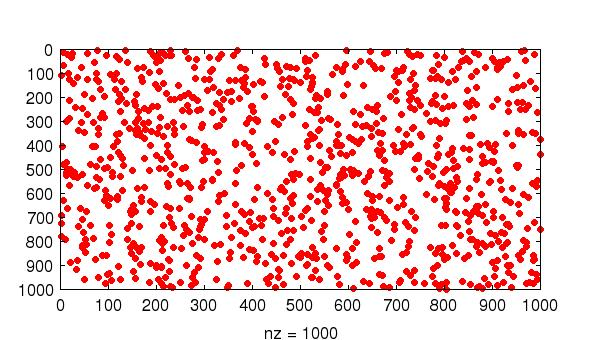
\includegraphics[width=8cm]{spy1}}

Here is a sparse matrix with a little more structure.  First we build a 
sparse matrix with block diagonal structure, and then use \verb|spy| to 
visualize the structure.
\begin{verbatim}
--> A = sparse(1000,1000);
--> for i=1:25; A((1:40) + 40*(i-1),(1:40) + 40*(i-1)) = 1; end;
--> spy(A,'gx')
\end{verbatim}
with the result shown here


\centerline{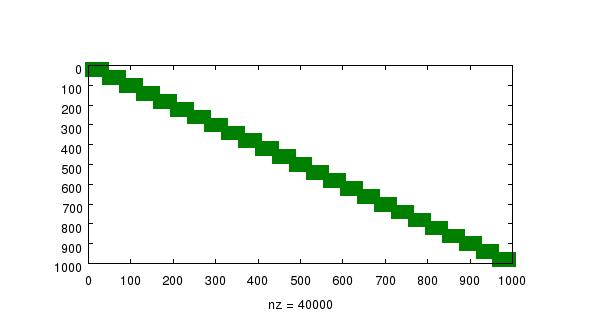
\includegraphics[width=8cm]{spy2}}


\chapter{Mathematical Functions}
\section{ACOS Inverse Trigonometric Arccosine Function}

\subsection{Usage}

Computes the \verb|acos| function for its argument.  The general
syntax for its use is
\begin{verbatim}
  y = acos(x)
\end{verbatim}
where \verb|x| is an \verb|n|-dimensional array of numerical type.
Integer types are promoted to the \verb|double| type prior to
calculation of the \verb|acos| function.  Output \verb|y| is of the
same size and type as the input \verb|x|, (unless \verb|x| is an
integer, in which case \verb|y| is a \verb|double| type).  
\subsection{Function Internals}

Mathematically, the \verb|acos| function is defined for all 
arguments \verb|x| as
\[
 \mathrm{acos} x \equiv \frac{pi}{2} + i \log \left(i x + 
  \sqrt{1-x^2}\right).
\]
For real valued variables \verb|x| in the range \verb|[-1,1]|, the function is
computed directly using the standard C library's numerical \verb|acos|
function. For both real and complex arguments \verb|x|, note that generally
\[
  \mathrm{acos}(\cos(x)) \neq x,
\]
\subsection{Example}

The following code demonstates the \verb|acos| function over the range 
\verb|[-1,1]|.
@>


\centerline{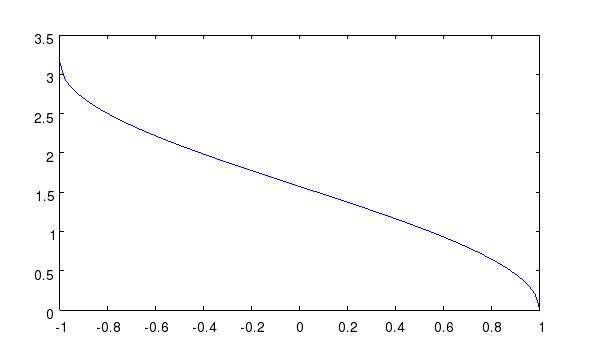
\includegraphics[width=8cm]{acosplot}}


\section{ACOSD Inverse Cosine Degrees Function}

\subsection{Usage}

Computes the inverse cosine of the argument, but returns
the argument in degrees instead of radians (as is the case
for \verb|acos|. The syntax for its use is
\begin{verbatim}
   y = acosd(x)
\end{verbatim}
\subsection{Examples}

The inverse cosine of \verb|sqrt(2)/2| should be 45 degrees:
\begin{verbatim}
--> acosd(sqrt(2)/2)

ans = 
  45.0000 +  0.0000i 
\end{verbatim}
and the inverse cosine of \verb|0.5| should be 60 degrees:
\begin{verbatim}
--> acosd(0.5)

ans = 
  60.0000 +  0.0000i 
\end{verbatim}

\section{ACOSH Inverse Hyperbolic Cosine Function}

\subsection{Usage}

Computes the inverse hyperbolic cosine of its argument.  The general
syntax for its use is
\begin{verbatim}
  y = acosh(x)
\end{verbatim}
where \verb|x| is an \verb|n|-dimensional array of numerical type.
\subsection{Function Internals}

The \verb|acosh| function is computed from the formula
\[
   \cosh^{-1}(x) = \log\left(x + (x^2 - 1)^0.5\right)
\]
where the \verb|log| (and square root) is taken in its most general sense.
\subsection{Examples}

Here is a simple plot of the inverse hyperbolic cosine function
@>


\centerline{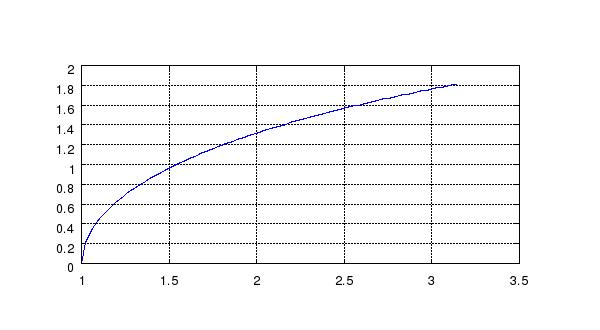
\includegraphics[width=8cm]{acoshplot}}


\section{ACOT Inverse Cotangent Function}

\subsection{Usage}

Computes the inverse cotangent of its argument.  The general
syntax for its use is
\begin{verbatim}
  y = acot(x)
\end{verbatim}
where \verb|x| is an \verb|n|-dimensional array of numerical type.
\subsection{Function Internals}

The \verb|acot| function is computed from the formula
\[
   \cot^{-1}(x) = \tan^{-1}\left(\frac{1}{x}\right)
\]
\subsection{Examples}

Here is a simple plot of the inverse cotangent function
\begin{verbatim}
--> x1 = -2*pi:pi/30:-0.1;
--> x2 = 0.1:pi/30:2*pi;
--> plot(x1,acot(x1),x2,acot(x2)); grid('on');
\end{verbatim}


\centerline{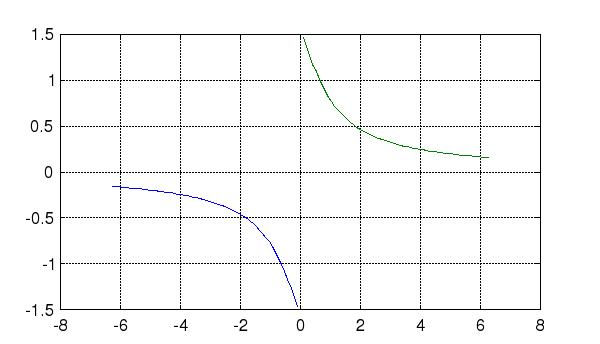
\includegraphics[width=8cm]{acotplot}}


\section{ACOTD Inverse Cotangent Degrees Function}

\subsection{Usage}

Computes the inverse cotangent of its argument in degrees.  The general
syntax for its use is
\begin{verbatim}
  y = acotd(x)
\end{verbatim}
where \verb|x| is an \verb|n|-dimensional array of numerical type.

\section{ACOTH Inverse Hyperbolic Cotangent Function}

\subsection{Usage}

Computes the inverse hyperbolic cotangent of its argument.  The general
syntax for its use is
\begin{verbatim}
  y = acoth(x)
\end{verbatim}
where \verb|x| is an \verb|n|-dimensional array of numerical type.
\subsection{Function Internals}

The \verb|acoth| function is computed from the formula
\[
   \coth^{-1}(x) = \tanh^{-1}\left(\frac{1}{x}\right)
\]
\subsection{Examples}

Here is a simple plot of the inverse hyperbolic cotangent function
@>


\centerline{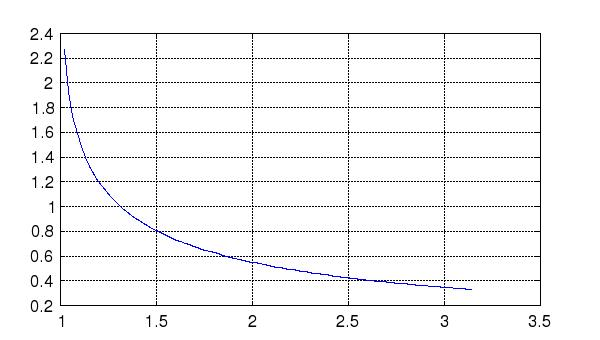
\includegraphics[width=8cm]{acothplot}}


\section{ACSC Inverse Cosecant Function}

\subsection{Usage}

Computes the inverse cosecant of its argument.  The general
syntax for its use is
\begin{verbatim}
  y = acsc(x)
\end{verbatim}
where \verb|x| is an \verb|n|-dimensional array of numerical type.
\subsection{Function Internals}

The \verb|acosh| function is computed from the formula
\[
   \csc^{-1}(x) = \sin^{-1}\left(\frac{1}{x}\right)
\]
\subsection{Examples}

Here is a simple plot of the inverse cosecant function
@>


\centerline{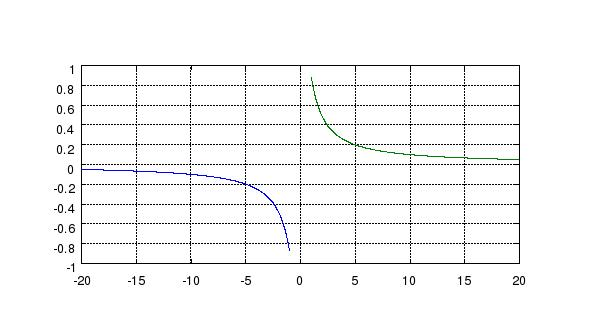
\includegraphics[width=8cm]{acschplot}}


\section{ACSCD Inverse Cosecant Degrees Function}

\subsection{Usage}

Computes the inverse cosecant of the argument, but returns
the argument in degrees instead of radians (as is the case
for \verb|acsc|. The syntax for its use is
\begin{verbatim}
   y = acscd(x)
\end{verbatim}
\subsection{Examples}

The inverse cosecant of \verb|2/sqrt(2)| should be 45 degrees:
@>
and the inverse cosecant of \verb|2| should be 30 degrees:
@>

\section{ACSCH Inverse Hyperbolic Cosecant Function}

\subsection{Usage}

Computes the inverse hyperbolic cosecant of its argument.  The general
syntax for its use is
\begin{verbatim}
  y = acsch(x)
\end{verbatim}
where \verb|x| is an \verb|n|-dimensional array of numerical type.
\subsection{Function Internals}

The \verb|acsch| function is computed from the formula
\[
   \mathrm{csch}^{-1}(x) = \sinh^{-1}\left(\frac{1}{x}\right)
\]
\subsection{Examples}

Here is a simple plot of the inverse hyperbolic cosecant function
\begin{verbatim}
--> x1 = -20:.01:-1;
--> x2 = 1:.01:20;
--> plot(x1,acsch(x1),x2,acsch(x2)); grid('on');
\end{verbatim}


\centerline{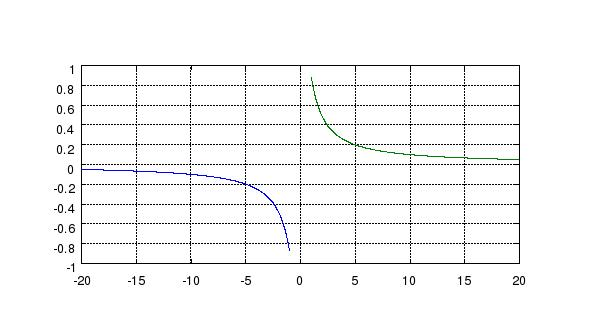
\includegraphics[width=8cm]{acschplot}}


\section{ANGLE Phase Angle Function
}

\subsection{Usage}

Compute the phase angle in radians of a complex matrix.  The general
syntax for its use is
\begin{verbatim}
  p = angle(c)
\end{verbatim}
where \verb|c| is an \verb|n|-dimensional array of numerical type.
\subsection{Function Internals}

For a complex number \verb|x|, its polar representation is
given by
\[
  x = |x| e^{j\theta}
\]
and we can compute 
\[
  \theta = \mathrm{atan2}(\Im x, \Re x)
\]
\subsection{Example}

Here are some examples of the use of \verb|angle| in the polar decomposition
of a complex number.
@>
   M version contributor: M.W. Vogel 01-30-06

\section{ASEC Inverse Secant Function}

\subsection{Usage}

Computes the inverse secant of its argument.  The general
syntax for its use is
\begin{verbatim}
  y = asec(x)
\end{verbatim}
where \verb|x| is an \verb|n|-dimensional array of numerical type.
\subsection{Function Internals}

The \verb|acosh| function is computed from the formula
\[
   \sec^{-1}(x) = \cos^{-1}\left(\frac{1}{x}\right)
\]
\subsection{Examples}

Here is a simple plot of the inverse secant function
\begin{verbatim}
--> x1 = -5:.01:-1;
--> x2 = 1:.01:5;
--> plot(x1,asec(x1),x2,asec(x2)); grid('on');
\end{verbatim}


\centerline{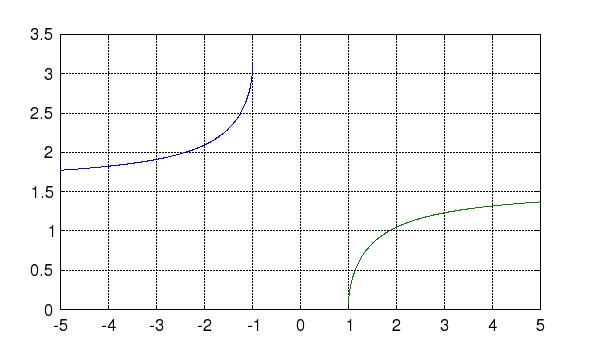
\includegraphics[width=8cm]{asecplot}}


\section{ASECD Inverse Secant Degrees Function}

\subsection{Usage}

Computes the inverse secant of the argument, but returns
the argument in degrees instead of radians (as is the case
for \verb|asec|. The syntax for its use is
\begin{verbatim}
   y = asecd(x)
\end{verbatim}
\subsection{Examples}

The inverse secant of \verb|2/sqrt(2)| should be 45 degrees:
\begin{verbatim}
--> asecd(2/sqrt(2))

ans = 

  45.0000 +  0.0000i 
\end{verbatim}
and the inverse secant of \verb|2| should be 60 degrees:
\begin{verbatim}
--> asecd(2)

ans = 

  60.0000 +  0.0000i 
\end{verbatim}

\section{ASECH Inverse Hyperbolic Secant Function}

\subsection{Usage}

Computes the inverse hyperbolic secant of its argument.  The general
syntax for its use is
\begin{verbatim}
  y = asech(x)
\end{verbatim}
where \verb|x| is an \verb|n|-dimensional array of numerical type.
\subsection{Function Internals}

The \verb|asech| function is computed from the formula
\[
   \mathrm{sech}^{-1}(x) = \cosh^{-1}\left(\frac{1}{x}\right)
\]
\subsection{Examples}

Here is a simple plot of the inverse hyperbolic secant function
\begin{verbatim}
--> x1 = -20:.01:-1;
--> x2 = 1:.01:20;
--> plot(x1,imag(asech(x1)),x2,imag(asech(x2))); grid('on');
\end{verbatim}


\centerline{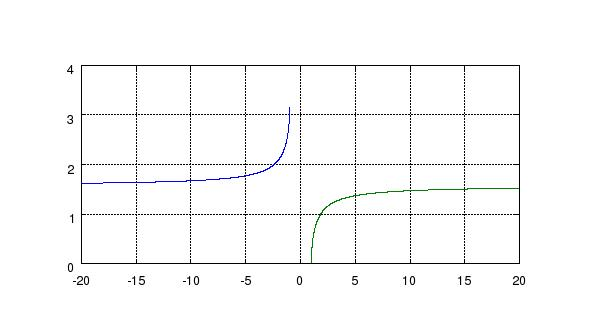
\includegraphics[width=8cm]{asechplot}}


\section{ASIN Inverse Trigonometric Arcsine Function}

\subsection{Usage}

Computes the \verb|asin| function for its argument.  The general
syntax for its use is
\begin{verbatim}
  y = asin(x)
\end{verbatim}
where \verb|x| is an \verb|n|-dimensional array of numerical type.
Integer types are promoted to the \verb|double| type prior to
calculation of the \verb|asin| function.  Output \verb|y| is of the
same size and type as the input \verb|x|, (unless \verb|x| is an
integer, in which case \verb|y| is a \verb|double| type).  
\subsection{Function Internals}

Mathematically, the \verb|asin| function is defined for all 
arguments \verb|x| as
\[
   \mathrm{asin} x \equiv - i \log \left(i x + 
   \sqrt{1-x^2}\right).
\]
For real valued variables \verb|x| in the range \verb|[-1,1]|, the function is
computed directly using the standard C library's numerical \verb|asin|
function. For both real and complex arguments \verb|x|, note that generally
\[
   \mathrm{asin}(\sin(x)) \neq x,
\]
due to the periodicity of \verb|sin(x)|.
\subsection{Example}

The following code demonstates the \verb|asin| function over the range 
\verb|[-1,1]|.
\begin{verbatim}
--> t = linspace(-1,1);
--> plot(t,asin(t))
\end{verbatim}


\centerline{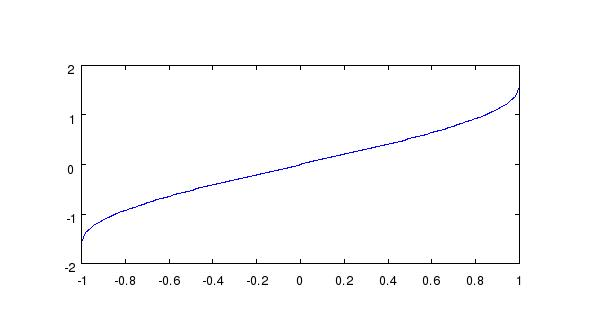
\includegraphics[width=8cm]{asinplot}}


\section{ASIND Inverse Sine Degrees Function}

\subsection{Usage}

Computes the inverse sine of the argument, but returns
the argument in degrees instead of radians (as is the case
for \verb|asin|). The syntax for its use is
\begin{verbatim}
   y = asind(x)
\end{verbatim}
\subsection{Examples}

The inverse sine of \verb|sqrt(2)/2| should be 45 degrees:
@>
and the inverse sine of \verb|0.5| should be 30 degrees:
@>

\section{ASINH Inverse Hyperbolic Sine Function}

\subsection{Usage}

Computes the inverse hyperbolic sine of its argument.  The general
syntax for its use is
\begin{verbatim}
  y = asinh(x)
\end{verbatim}
where \verb|x| is an \verb|n|-dimensional array of numerical type.
\subsection{Function Internals}

The \verb|asinh| function is computed from the formula
\[
   \sinh^{-1}(x) = \log\left(x + (x^2 + 1)^0.5\right)
\]
where the \verb|log| (and square root) is taken in its most general sense.
\subsection{Examples}

Here is a simple plot of the inverse hyperbolic sine function
@>


\centerline{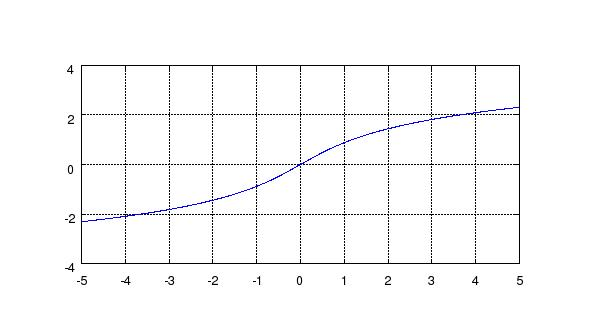
\includegraphics[width=8cm]{asinhplot}}


\section{ATAN Inverse Trigonometric Arctangent Function}

\subsection{Usage}

Computes the \verb|atan| function for its argument.  The general
syntax for its use is
\begin{verbatim}
  y = atan(x)
\end{verbatim}
where \verb|x| is an \verb|n|-dimensional array of numerical type.
Integer types are promoted to the \verb|double| type prior to
calculation of the \verb|atan| function.  Output \verb|y| is of the
same size and type as the input \verb|x|, (unless \verb|x| is an
integer, in which case \verb|y| is a \verb|double| type).  
\subsection{Function Internals}

Mathematically, the \verb|atan| function is defined for all 
arguments \verb|x| as
\[
   \mathrm{atan} x \equiv \frac{i}{2}\left(\log(1-i x) - \log(i x + 1)\right).
\]
For real valued variables \verb|x|, the function is computed directly using 
the standard C library's numerical \verb|atan| function. For both 
real and complex arguments \verb|x|, note that generally

\[
    \mathrm{atan}(\tan(x)) \neq x,
\]
 due to the periodicity of \verb|tan(x)|.
\subsection{Example}

The following code demonstates the \verb|atan| function over the range 
\verb|[-1,1]|.
\begin{verbatim}
--> t = linspace(-1,1);
--> plot(t,atan(t))
\end{verbatim}


\centerline{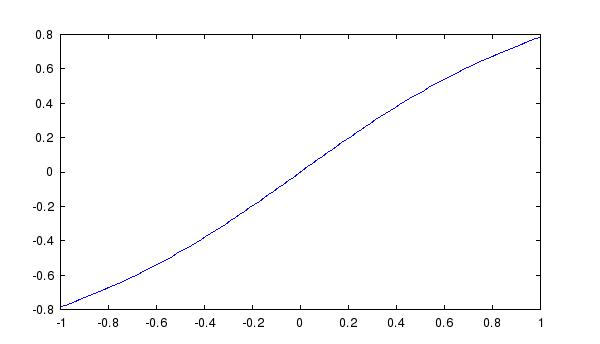
\includegraphics[width=8cm]{atanplot}}


\section{ATAN2 Inverse Trigonometric 4-Quadrant Arctangent Function}

\subsection{Usage}

Computes the \verb|atan2| function for its argument.  The general
syntax for its use is
\begin{verbatim}
  z = atan2(y,x)
\end{verbatim}
where \verb|x| and \verb|y| are \verb|n|-dimensional arrays of numerical type.
Integer types are promoted to the \verb|double| type prior to
calculation of the \verb|atan2| function. The size of the output depends
on the size of \verb|x| and \verb|y|.  If \verb|x| is a scalar, then \verb|z|
is the same size as \verb|y|, and if \verb|y| is a scalar, then \verb|z|
is the same size as \verb|x|.  The type of the output is equal to the type of
|y/x|.  
\subsection{Function Internals}

The function is defined (for real values) to return an 
angle between \verb|-pi| and \verb|pi|.  The signs of \verb|x| and \verb|y|
are used to find the correct quadrant for the solution.  For complex
arguments, the two-argument arctangent is computed via
\[
  \mathrm{atan2}(y,x) \equiv -i \log\left(\frac{x+i y}{\sqrt{x^2+y^2}} \right)
\]
For real valued arguments \verb|x,y|, the function is computed directly using 
the standard C library's numerical \verb|atan2| function. For both 
real and complex arguments \verb|x|, note that generally
\[
  \mathrm{atan2}(\sin(x),\cos(x)) \neq x,
\]
due to the periodicities of  \verb|cos(x)| and \verb|sin(x)|.
\subsection{Example}

The following code demonstates the difference between the \verb|atan2| 
function and the \verb|atan| function over the range \verb|[-pi,pi]|.
\begin{verbatim}
--> x = linspace(-pi,pi);
--> sx = sin(x); cx = cos(x);
--> plot(x,atan(sx./cx),x,atan2(sx,cx))
\end{verbatim}


\centerline{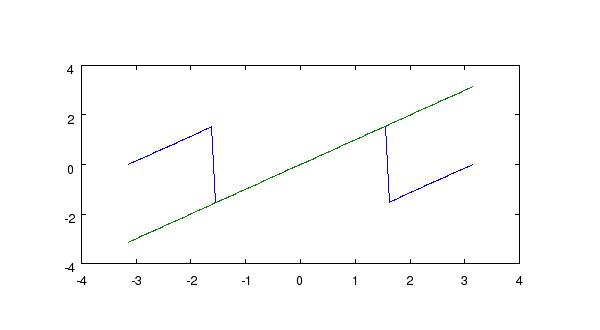
\includegraphics[width=8cm]{atan2plot}}

Note how the two-argument \verb|atan2| function (green line) 
correctly ``unwraps'' the phase of the angle, while the \verb|atan| 
function (red line) wraps the angle to the interval \verb|[-\pi/2,\pi/2]|.

\section{ATAND Inverse Tangent Degrees Function}

\subsection{Usage}

Computes the inverse tangent of the argument, but returns
the argument in degrees instead of radians (as is the case
for \verb|atan|. The syntax for its use is
\begin{verbatim}
   y = atand(x)
\end{verbatim}
\subsection{Examples}

The inverse tangent of \verb|1| should be 45 degrees:
\begin{verbatim}
--> atand(1)

ans = 
 45 
\end{verbatim}

\section{ATANH Inverse Hyperbolic Tangent Function}

\subsection{Usage}

Computes the inverse hyperbolic tangent of its argument.  The general
syntax for its use is
\begin{verbatim}
  y = atanh(x)
\end{verbatim}
where \verb|x| is an \verb|n|-dimensional array of numerical type.
\subsection{Function Internals}

The \verb|atanh| function is computed from the formula
\[
   \tanh^{-1}(x) = \frac{1}{2}\log\left(\frac{1+x}{1-x}\right)
\]
where the \verb|log| (and square root) is taken in its most general sense.
\subsection{Examples}

Here is a simple plot of the inverse hyperbolic tangent function
\begin{verbatim}
--> x = -0.99:.01:0.99;
--> plot(x,atanh(x)); grid('on');
\end{verbatim}


\centerline{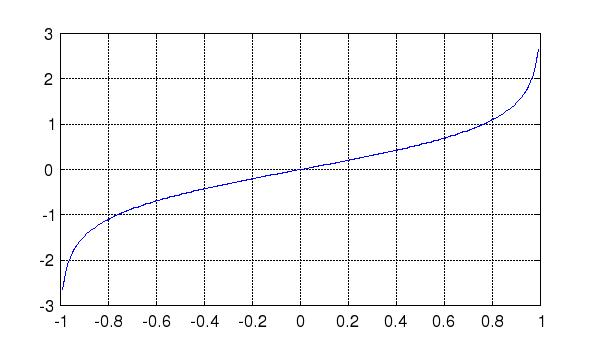
\includegraphics[width=8cm]{atanhplot}}


\section{COS Trigonometric Cosine Function}

\subsection{Usage}

Computes the \verb|cos| function for its argument.  The general
syntax for its use is
\begin{verbatim}
  y = cos(x)
\end{verbatim}
where \verb|x| is an \verb|n|-dimensional array of numerical type.
Integer types are promoted to the \verb|double| type prior to
calculation of the \verb|cos| function.  Output \verb|y| is of the
same size and type as the input \verb|x|, (unless \verb|x| is an
integer, in which case \verb|y| is a \verb|double| type).  
\subsection{Function Internals}

Mathematically, the \verb|cos| function is defined for all real
valued arguments \verb|x| by the infinite summation
\[
  \cos x \equiv \sum_{n=0}^{\infty} \frac{(-1)^n x^{2n}}{(2n)!}.
\]
For complex valued arguments \verb|z|, the cosine is computed via
\[
  \cos z \equiv \cos \Re z \cosh \Im z - \sin \Re z
  \sinh \Im z.
\]
\subsection{Example}

The following piece of code plots the real-valued \verb|cos(2 pi x)|
function over one period of \verb|[0,1]|:
@>


\centerline{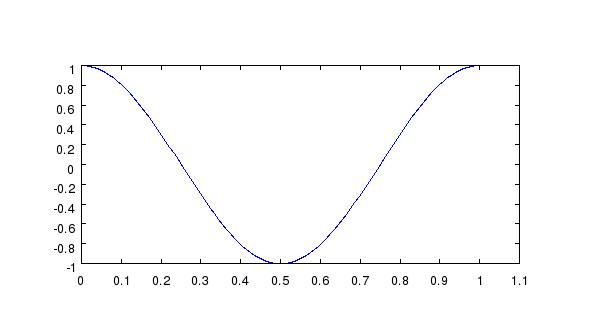
\includegraphics[width=8cm]{cosplot}}


\section{COSD Cosine Degrees Function}

\subsection{Usage}

Computes the cosine of the argument, but takes
the argument in degrees instead of radians (as is the case
for \verb|cos|). The syntax for its use is
\begin{verbatim}
   y = cosd(x)
\end{verbatim}
\subsection{Examples}

The cosine of 45 degrees should be \verb|sqrt(2)/2|
\begin{verbatim}
--> cosd(45)

ans = 

    0.7071 
\end{verbatim}
and the cosine of \verb|60| degrees should be 0.5:
\begin{verbatim}
--> cosd(60)

ans = 

    0.5000 
\end{verbatim}

\section{COSH Hyperbolic Cosine Function}

\subsection{Usage}

Computes the hyperbolic cosine of the argument.
The syntax for its use is
\begin{verbatim}
   y = cosh(x)
\end{verbatim}
\subsection{Function Internals}

The \verb|cosh| function is computed from the formula
\[
   \cosh(x) = \frac{e^x+e^{-x}}{2}
\]
For \verb|x| complex, it follows that
\[
   \cosh(a+i*b) = \frac{e^a(\cos(b)+i*\sin(b)) + e^{-a}(\cos(-b)+i*\sin(-b))}{2}
\]
\subsection{Examples}

Here is a simple plot of the hyperbolic cosine function
\begin{verbatim}
--> x = linspace(-5,5);
--> plot(x,cosh(x)); grid('on');
\end{verbatim}


\centerline{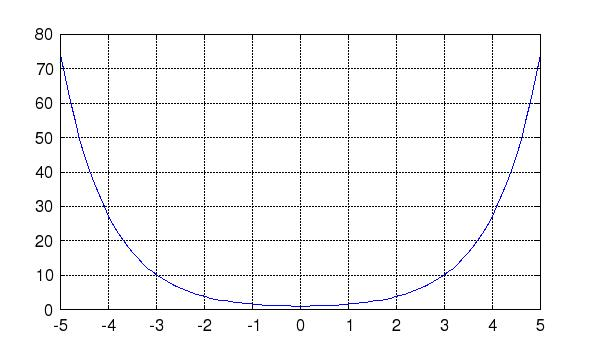
\includegraphics[width=8cm]{coshplot}}


\section{COT Trigonometric Cotangent Function}

\subsection{Usage}

Computes the \verb|cot| function for its argument.  The general
syntax for its use is
\begin{verbatim}
  y = cot(x)
\end{verbatim}
where \verb|x| is an \verb|n|-dimensional array of numerical type.
Integer types are promoted to the \verb|double| type prior to
calculation of the \verb|cot| function.  Output \verb|y| is of the
same size and type as the input \verb|x|, (unless \verb|x| is an
integer, in which case \verb|y| is a \verb|double| type).  
\subsection{Function Internals}

Mathematically, the \verb|cot| function is defined for all 
arguments \verb|x| as
\[
  \cot x \equiv \frac{\cos x}{\sin x}
\]
For complex valued arguments \verb|z|, the cotangent is computed via
\[
  \cot z \equiv \frac{\cos 2 \Re z + \cosh 2 \Im z}{\sin 2 \Re z + 
  i \sinh 2 \Im z}.
\]
\subsection{Example}

The following piece of code plots the real-valued \verb|cot(x)|
function over the interval \verb|[-1,1]|:
@>


\centerline{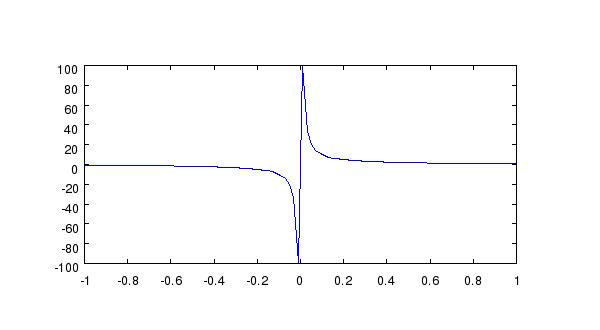
\includegraphics[width=8cm]{cotplot}}


\section{COTD Cotangent Degrees Function}

\subsection{Usage}

Computes the cotangent of the argument, but takes
the argument in degrees instead of radians (as is the case
for \verb|cot|). The syntax for its use is
\begin{verbatim}
   y = cotd(x)
\end{verbatim}
\subsection{Examples}

The cotangent of 45 degrees should be 1.
\begin{verbatim}
--> cotd(45)

ans = 
 1 
\end{verbatim}

\section{COTD Cotangent Degrees Function}

\subsection{Usage}

Computes the cotangent of the argument, but takes
the argument in degrees instead of radians (as is the case
for \verb|cot|). The syntax for its use is
\begin{verbatim}
   y = cotd(x)
\end{verbatim}
\subsection{Examples}

The cotangent of 45 degrees should be 1.
\begin{verbatim}
--> cotd(45)

ans = 
 1 
\end{verbatim}

\section{COTH Hyperbolic Cotangent Function}

\subsection{Usage}

Computes the hyperbolic cotangent of the argument.
The syntax for its use is
\begin{verbatim}
   y = coth(x)
\end{verbatim}
\subsection{Function Internals}

The \verb|coth| function is computed from the formula
\[
   \coth(x) = \frac{1}{\tanh(x)}
\]
\subsection{Examples}

Here is a simple plot of the hyperbolic cotangent function
@>


\centerline{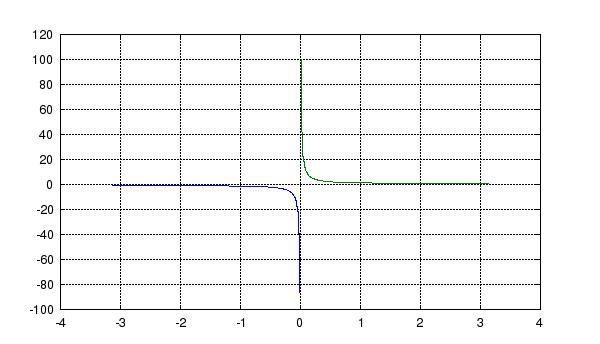
\includegraphics[width=8cm]{cothplot}}


\section{CROSS Cross Product of Two Vectors}

\subsection{Usage}

Computes the cross product of two vectors.  The general syntax
for its use is
\begin{verbatim}
    c = cross(a,b)
\end{verbatim}
where \verb|a| and \verb|b| are 3-element vectors.

\section{CSC Trigonometric Cosecant Function}

\subsection{Usage}

Computes the \verb|csc| function for its argument.  The general
syntax for its use is
\begin{verbatim}
  y = csc(x)
\end{verbatim}
where \verb|x| is an \verb|n|-dimensional array of numerical type.
Integer types are promoted to the \verb|double| type prior to
calculation of the \verb|csc| function.  Output \verb|y| is of the
same size and type as the input \verb|x|, (unless \verb|x| is an
integer, in which case \verb|y| is a \verb|double| type).  
\subsection{Function Internals}

Mathematically, the \verb|csc| function is defined for all arguments
as
\[
   \csc x \equiv \frac{1}{\sin x}.
\]
\subsection{Example}

The following piece of code plots the real-valued \verb|csc(2 pi x)|
function over the interval of \verb|[-1,1]|:
\begin{verbatim}
--> t = linspace(-1,1,1000);
--> plot(t,csc(2*pi*t))
--> axis([-1,1,-10,10]);
\end{verbatim}


\centerline{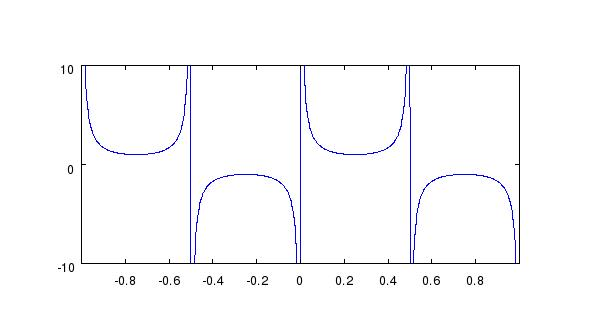
\includegraphics[width=8cm]{cscplot}}


\section{CSCD Cosecant Degrees Function}

\subsection{Usage}

Computes the cosecant of the argument, but takes
the argument in degrees instead of radians (as is the case
for \verb|csc|). The syntax for its use is
\begin{verbatim}
   y = cscd(x)
\end{verbatim}

\section{CSCH Hyperbolic Cosecant Function}

\subsection{Usage}

Computes the hyperbolic cosecant of the argument.
The syntax for its use is
\begin{verbatim}
   y = csch(x)
\end{verbatim}
\subsection{Function Internals}

The \verb|csch| function is computed from the formula
\[
   \mathrm{csch}(x) = \frac{1}{\sinh(x)}
\]
\subsection{Examples}

Here is a simple plot of the hyperbolic cosecant function
\begin{verbatim}
--> x1 = -pi+.01:.01:-.01;
--> x2 = .01:.01:pi-.01;
--> plot(x1,csch(x1),x2,csch(x2)); grid('on');
\end{verbatim}


\centerline{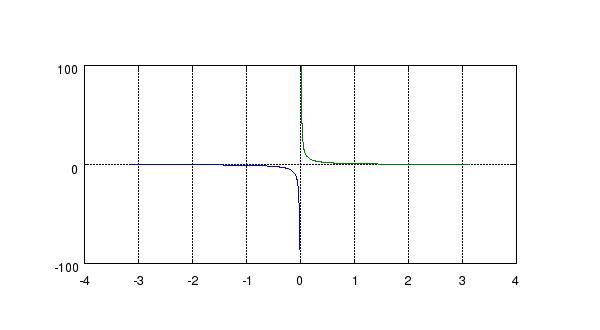
\includegraphics[width=8cm]{cschplot}}


\section{DEG2RAD Convert From Degrees To Radians}

\subsection{Usage}

Converts the argument from degrees to radians.  The
syntax for its use is
\begin{verbatim}
   y = deg2rad(x)
\end{verbatim}
where \verb|x| is a numeric array.  Conversion is done by
simply multiplying \verb|x| by \verb|pi/180|.
\subsection{Example}

How many radians in a circle:
\begin{verbatim}
--> deg2rad(360) - 2*pi

ans = 

 0 
\end{verbatim}

\section{ERF Error Function}

\subsection{Usage}

Computes the error function for real arguments.  The \verb|erf|
function takes only a single argument
\begin{verbatim}
  y = erf(x)
\end{verbatim}
where \verb|x| is either a \verb|float| or \verb|double| array.  The output
vector \verb|y| is the same size (and type) as \verb|x|.
\subsection{Function Internals}

The erf function is defined by the integral:
\[
  \mathrm{erf}(x) = \frac{2}{\sqrt{\pi}}\int_{0}^{x} e^{-t^2} \, dt,
\]
and is the integral of the normal distribution.
\subsection{Example}

Here is a plot of the erf function over the range \verb|[-5,5]|.
\begin{verbatim}
--> x = linspace(-5,5);
--> y = erf(x);
--> plot(x,y); xlabel('x'); ylabel('erf(x)');
\end{verbatim}
which results in the following plot.


\centerline{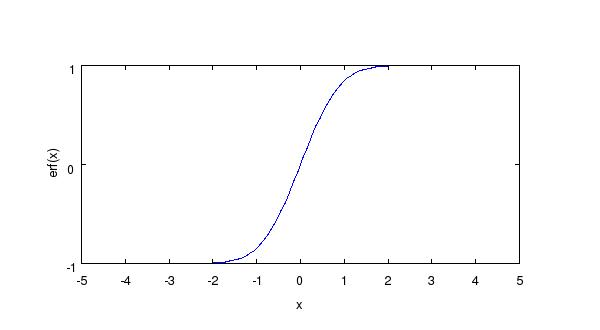
\includegraphics[width=8cm]{erf1}}


\section{ERFC Complimentary Error Function}

\subsection{Usage}

Computes the complimentary error function for real arguments.  The \verb|erfc|
function takes only a single argument
\begin{verbatim}
  y = erfc(x)
\end{verbatim}
where \verb|x| is either a \verb|float| or \verb|double| array.  The output
vector \verb|y| is the same size (and type) as \verb|x|.
\subsection{Function Internals}

The erfc function is defined by the integral:
\[
  \mathrm{erfc}(x) = \frac{2}{\sqrt{\pi}}\int_{x}^{\infty} e^{-t^2} \, dt,
\]
and is the integral of the normal distribution.
\subsection{Example}

Here is a plot of the \verb|erfc| function over the range \verb|[-5,5]|.
\begin{verbatim}
--> x = linspace(-5,5);
--> y = erfc(x);
--> plot(x,y); xlabel('x'); ylabel('erfc(x)');
\end{verbatim}
which results in the following plot.


\centerline{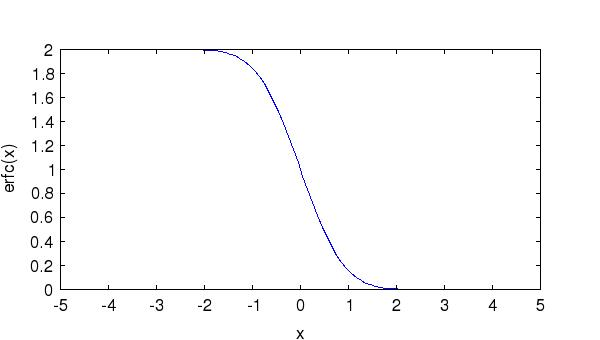
\includegraphics[width=8cm]{erfc1}}


\section{EXP Exponential Function}

\subsection{Usage}

Computes the \verb|exp| function for its argument.  The general
syntax for its use is
\begin{verbatim}
   y = exp(x)
\end{verbatim}
where \verb|x| is an \verb|n|-dimensional array of numerical type.
Integer types are promoted to the \verb|double| type prior to
calculation of the \verb|exp| function.  Output \verb|y| is of the
same size and type as the input \verb|x|, (unless \verb|x| is an
integer, in which case \verb|y| is a \verb|double| type).
\subsection{Function Internals}

Mathematically, the \verb|exp| function is defined for all real
valued arguments \verb|x| as
\[
  \exp x \equiv e^{x},
\]
where
\[
  e = \sum_{0}^{\infty} \frac{1}{k!}
\]
and is approximately \verb|2.718281828459045| (returned by the function 
\verb|e|).  For complex values
\verb|z|, the famous Euler formula is used to calculate the 
exponential
\[
  e^{z} = e^{|z|} \left[ \cos \Re z + i \sin \Re z \right]
\]
\subsection{Example}

The following piece of code plots the real-valued \verb|exp|
function over the interval \verb|[-1,1]|:
\begin{verbatim}
--> x = linspace(-1,1);
--> plot(x,exp(x))
\end{verbatim}


\centerline{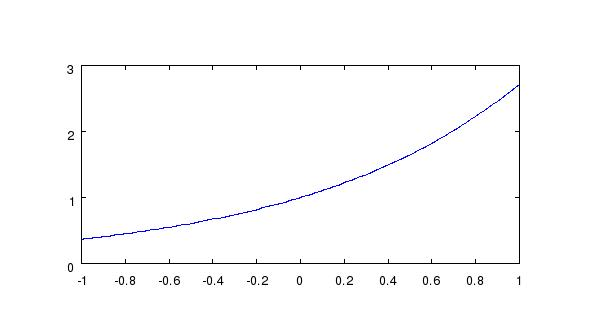
\includegraphics[width=8cm]{expplot1}}

In the second example, we plot the unit circle in the 
complex plane \verb|e^{i 2 pi x}| for \verb|x in [-1,1]|.
\begin{verbatim}
--> x = linspace(-1,1);
--> plot(exp(-i*x*2*pi))
\end{verbatim}


\centerline{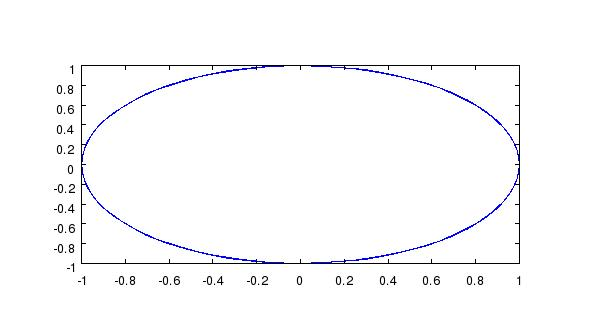
\includegraphics[width=8cm]{expplot2}}


\section{EXPM1 Exponential Minus One Function}

\subsection{Usage}

Computes \verb|exp(x)-1| function accurately for \verb|x|
small.  The syntax for its use is
\begin{verbatim}
   y = expm1(x)
\end{verbatim}
where \verb|x| is an \verb|n|-dimensional array of numerical type.

\section{FIX Round Towards Zero}

\subsection{Usage}

Rounds the argument array towards zero.  The syntax for its use is
\begin{verbatim}
   y = fix(x)
\end{verbatim}
where \verb|x| is a numeric array.  For positive elements of \verb|x|, the output
is the largest integer smaller than \verb|x|.  For negative elements of \verb|x|
the output is the smallest integer larger than \verb|x|.  For complex \verb|x|,
the operation is applied seperately to the real and imaginary parts.
\subsection{Example}

Here is a simple example of the \verb|fix| operation on some values
@>

\section{GAMMA Gamma Function}

\subsection{Usage}

Computes the gamma function for real arguments.  The \verb|gamma|
function takes only a single argument
\begin{verbatim}
  y = gamma(x)
\end{verbatim}
where \verb|x| is either a \verb|float| or \verb|double| array.  The output
vector \verb|y| is the same size (and type) as \verb|x|.
\subsection{Function Internals}

The gamma function is defined by the integral:
\[
  \Gamma(x) = \int_{0}^{\infty} e^{-t} t^{x-1} \, dt
\]
The gamma function obeys the interesting relationship
\[
  \Gamma(x) = (x-1)\Gamma(x-1),
\]
and for integer arguments, is equivalent to the factorial function.
\subsection{Example}

Here is a plot of the gamma function over the range \verb|[-5,5]|.
\begin{verbatim}
--> x = linspace(-5,5);
--> y = gamma(x);
--> plot(x,y); xlabel('x'); ylabel('gamma(x)');
--> axis([-5,5,-5,5]);
\end{verbatim}
which results in the following plot.


\centerline{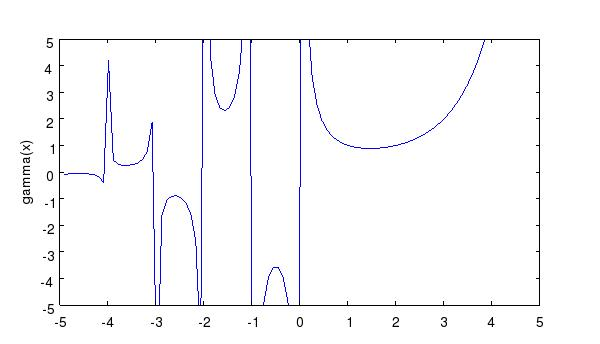
\includegraphics[width=8cm]{gamma1}}


\section{GAMMALN Log Gamma Function}

\subsection{Usage}

Computes the natural log of the gamma function for real arguments.  The \verb|gammaln|
function takes only a single argument
\begin{verbatim}
  y = gammaln(x)
\end{verbatim}
where \verb|x| is either a \verb|float| or \verb|double| array.  The output
vector \verb|y| is the same size (and type) as \verb|x|.
\subsection{Example}

Here is a plot of the \verb|gammaln| function over the range \verb|[-5,5]|.
@>
which results in the following plot.


\centerline{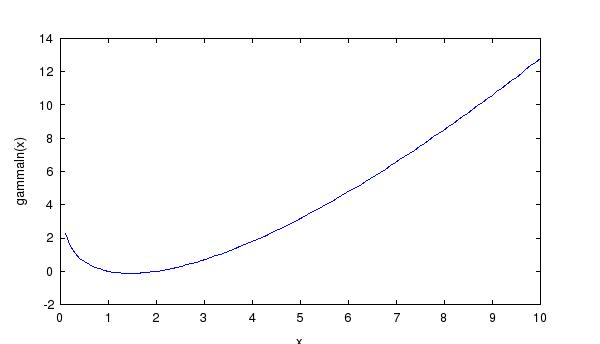
\includegraphics[width=8cm]{gammaln1}}


\section{IDIV Integer Division Operation}

\subsection{Usage}

Computes the integer division of two arrays.  The syntax for its use is
\begin{verbatim}
   y = idiv(a,b)
\end{verbatim}
where \verb|a| and \verb|b| are arrays or scalars.  The effect of the \verb|idiv|
is to compute the integer division of \verb|b| into \verb|a|.
\subsection{Example}

The following examples show some uses of \verb|idiv|
arrays.
\begin{verbatim}
--> idiv(27,6)

ans = 
 4 

--> idiv(4,-2)

ans = 
 -2 

--> idiv(15,3)

ans = 
 5 
\end{verbatim}

\section{LOG Natural Logarithm Function}

\subsection{Usage}

Computes the \verb|log| function for its argument.  The general
syntax for its use is
\begin{verbatim}
  y = log(x)
\end{verbatim}
where \verb|x| is an \verb|n|-dimensional array of numerical type.
Integer types are promoted to the \verb|double| type prior to
calculation of the \verb|log| function.  Output \verb|y| is of the
same size as the input \verb|x|. For strictly positive, real inputs, 
the output type is the same as the input.
For negative and complex arguments, the output is complex.
\subsection{Function Internals}

Mathematically, the \verb|log| function is defined for all real
valued arguments \verb|x| by the integral
\[
  \log x \equiv \int_1^{x} \frac{d\,t}{t}.
\]
For complex-valued arguments, \verb|z|, the complex logarithm is
defined as
\[
  \log z \equiv \log |z| + i \arg z,
\]
where \verb|arg| is the complex argument of \verb|z|.
\subsection{Example}

The following piece of code plots the real-valued \verb|log|
function over the interval \verb|[1,100]|:
\begin{verbatim}
--> x = linspace(1,100);
--> plot(x,log(x))
--> xlabel('x');
--> ylabel('log(x)');
\end{verbatim}


\centerline{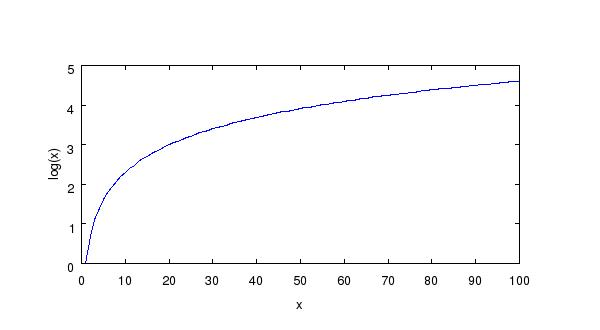
\includegraphics[width=8cm]{logplot}}


\section{LOG10 Base-10 Logarithm Function}

\subsection{Usage}

Computes the \verb|log10| function for its argument.  The general
syntax for its use is
\begin{verbatim}
  y = log10(x)
\end{verbatim}
where \verb|x| is an \verb|n|-dimensional array of numerical type.
Integer types are promoted to the \verb|double| type prior to
calculation of the \verb|log10| function.  Output \verb|y| is of the
same size as the input \verb|x|. For strictly positive, real inputs, 
the output type is the same as the input.
For negative and complex arguments, the output is complex.
\subsection{Example}

The following piece of code plots the real-valued \verb|log10|
function over the interval \verb|[1,100]|:
\begin{verbatim}
--> x = linspace(1,100);
--> plot(x,log10(x))
--> xlabel('x');
--> ylabel('log10(x)');
\end{verbatim}


\centerline{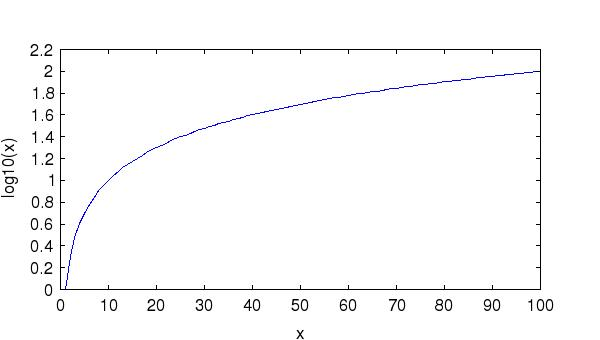
\includegraphics[width=8cm]{log10plot}}


\section{LOG1P Natural Logarithm of 1+P Function}

\subsection{Usage}

Computes the \verb|log| function for one plus its argument.  The general
syntax for its use is
\begin{verbatim}
  y = log1p(x)
\end{verbatim}
where \verb|x| is an \verb|n|-dimensional array of numerical type.

\section{LOG2 Base-2 Logarithm Function}

\subsection{Usage}

Computes the \verb|log2| function for its argument.  The general
syntax for its use is
\begin{verbatim}
  y = log2(x)
\end{verbatim}
where \verb|x| is an \verb|n|-dimensional array of numerical type.
Integer types are promoted to the \verb|double| type prior to
calculation of the \verb|log2| function.  Output \verb|y| is of the
same size as the input \verb|x|. For strictly positive, real inputs, 
the output type is the same as the input.
For negative and complex arguments, the output is complex.
\subsection{Example}

The following piece of code plots the real-valued \verb|log2|
function over the interval \verb|[1,100]|:
\begin{verbatim}
--> x = linspace(1,100);
--> plot(x,log2(x))
--> xlabel('x');
--> ylabel('log2(x)');
\end{verbatim}


\centerline{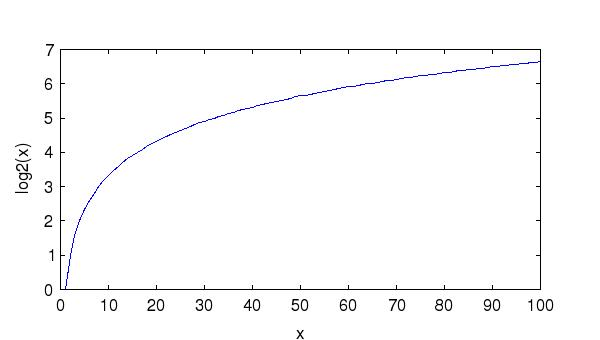
\includegraphics[width=8cm]{log2plot}}


\section{MOD Modulus Operation}

\subsection{Usage}

Computes the modulus of an array.  The syntax for its use is
\begin{verbatim}
   y = mod(x,n)
\end{verbatim}
where \verb|x| is matrix, and \verb|n| is the base of the modulus.  The
effect of the \verb|mod| operator is to add or subtract multiples of \verb|n|
to the vector \verb|x| so that each element \verb|x_i| is between \verb|0| and \verb|n|
(strictly).  Note that \verb|n| does not have to be an integer.  Also,
\verb|n| can either be a scalar (same base for all elements of \verb|x|), or a
vector (different base for each element of \verb|x|).

Note that the following are defined behaviors:
\begin{enumerate}
\item  \verb|mod(x,0) = x|@

\item  \verb|mod(x,x) = 0|@

\item  \verb|mod(x,n)|@ has the same sign as \verb|n| for all other cases.

\end{enumerate}
\subsection{Example}

The following examples show some uses of \verb|mod|
arrays.
@>
Here is an example of using \verb|mod| to determine if integers are even
 or odd:
@>
Here we use the second form of \verb|mod|, with each element using a 
separate base.
@>

\section{MPOWER Matrix Power Function}

\subsection{Usage}

Computes the matrix power operator for two arrays.  It is an
M-file version of the \verb|^| operator.  The syntax for its use is
\begin{verbatim}
   y = mpower(a,b)
\end{verbatim}
where \verb|y=a^b|.  See the \verb|matrixpower| documentation for more
details on what this function actually does.

\section{POWER Element-wise Power Function}

\subsection{Usage}

Computes the element-wise power operator for two arrays.  It is an
M-file version of the \verb|.^| operator.  The syntax for its use is
\begin{verbatim}
   y = power(a,b)
\end{verbatim}
where \verb|y=a.^b|.  See the \verb|dotpower| documentation for more
details on what this function actually does.

\section{RAD2DEG Radians To Degrees Conversion Function}

\subsection{Usage}

Converts the argument array from radians to degrees.  The general
syntax for its use is
\begin{verbatim}
   y = rad2deg(x)
\end{verbatim}
Note that the output type will be the same as the input type, and that
complex arguments are allowed.  The output is not wrapped to \verb|[0,360)|.
\subsection{Examples}

Some known conversion factors
\begin{verbatim}
--> rad2deg(1) % one radian is about 57 degrees

ans = 
   57.2958 

--> rad2deg(pi/4) % should be 45 degrees

ans = 
 45 

--> rad2deg(2*pi) % Note that this is 360 not 0 degrees

ans = 
 360 
\end{verbatim}

\section{REM Remainder After Division}

\subsection{Usage}

Computes the remainder after division of an array.  The syntax for its use is
\begin{verbatim}
   y = rem(x,n)
\end{verbatim}
where \verb|x| is matrix, and \verb|n| is the base of the modulus.  The
effect of the \verb|rem| operator is to add or subtract multiples of \verb|n|
to the vector \verb|x| so that each element \verb|x_i| is between \verb|0| and \verb|n|
(strictly).  Note that \verb|n| does not have to be an integer.  Also,
\verb|n| can either be a scalar (same base for all elements of \verb|x|), or a
vector (different base for each element of \verb|x|).

Note that the following are defined behaviors:
\begin{enumerate}
\item  \verb|rem(x,0) = nan|@

\item  \verb|rem(x,x) = 0|@ for nonzero \verb|x|

\item  \verb|rem(x,n)|@ has the same sign as \verb|x| for all other cases.

\end{enumerate}
Note that \verb|rem| and \verb|mod| return the same value if \verb|x| and \verb|n|
are of the same sign.  But differ by \verb|n| if \verb|x| and \verb|y| have 
different signs.
\subsection{Example}

The following examples show some uses of \verb|rem|
arrays.
\begin{verbatim}
--> rem(18,12)

ans = 

 6 

--> rem(6,5)

ans = 

 1 

--> rem(2*pi,pi)

ans = 

 0 
\end{verbatim}
Here is an example of using \verb|rem| to determine if integers are even
 or odd:
\begin{verbatim}
--> rem([1,3,5,2],2)

ans = 

 1 1 1 0 
\end{verbatim}
Here we use the second form of \verb|rem|, with each element using a 
separate base.
\begin{verbatim}
--> rem([9 3 2 0],[1 0 2 2])

ans = 

         0       nan         0         0 
\end{verbatim}

\section{SEC Trigonometric Secant Function}

\subsection{Usage}

Computes the \verb|sec| function for its argument.  The general
syntax for its use is
\begin{verbatim}
  y = sec(x)
\end{verbatim}
where \verb|x| is an \verb|n|-dimensional array of numerical type.
Integer types are promoted to the \verb|double| type prior to
calculation of the \verb|sec| function.  Output \verb|y| is of the
same size and type as the input \verb|x|, (unless \verb|x| is an
integer, in which case \verb|y| is a \verb|double| type).  
\subsection{Function Internals}

Mathematically, the \verb|sec| function is defined for all arguments
as
\[
   \sec x \equiv \frac{1}{\cos x}.
\]
\subsection{Example}

The following piece of code plots the real-valued \verb|sec(2 pi x)|
function over the interval of \verb|[-1,1]|:
@>


\centerline{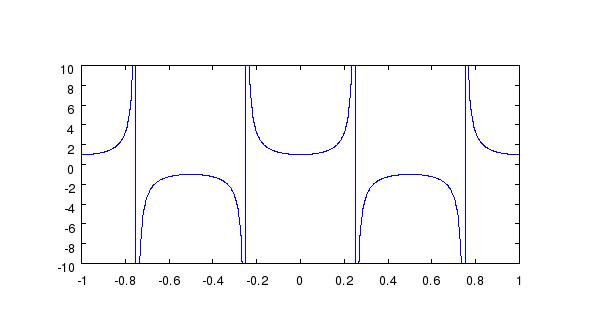
\includegraphics[width=8cm]{secplot}}


\section{SECD Secant Degrees Function}

\subsection{Usage}

Computes the secant of the argument, but takes
the argument in degrees instead of radians (as is the case
for \verb|sec|). The syntax for its use is
\begin{verbatim}
   y = secd(x)
\end{verbatim}

\section{SECH Hyperbolic Secant Function}

\subsection{Usage}

Computes the hyperbolic secant of the argument.
The syntax for its use is
\begin{verbatim}
   y = sech(x)
\end{verbatim}
\subsection{Function Internals}

The \verb|sech| function is computed from the formula
\[
   \mathrm{sech}(x) = \frac{1}{\cosh(x)}
\]
\subsection{Examples}

Here is a simple plot of the hyperbolic secant function
@>


\centerline{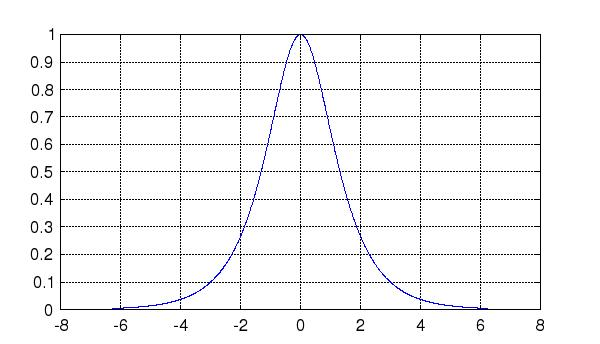
\includegraphics[width=8cm]{sechplot}}


\section{SIN Trigonometric Sine Function}

\subsection{Usage}

Computes the \verb|sin| function for its argument.  The general
syntax for its use is
\begin{verbatim}
  y = sin(x)
\end{verbatim}
where \verb|x| is an \verb|n|-dimensional array of numerical type.
Integer types are promoted to the \verb|double| type prior to
calculation of the \verb|sin| function.  Output \verb|y| is of the
same size and type as the input \verb|x|, (unless \verb|x| is an
integer, in which case \verb|y| is a \verb|double| type).  
\subsection{Function Internals}

Mathematically, the \verb|sin| function is defined for all real
valued arguments \verb|x| by the infinite summation
\[
  \sin x \equiv \sum_{n=1}^{\infty} \frac{(-1)^{n-1} x^{2n-1}}{(2n-1)!}.
\]
For complex valued arguments \verb|z|, the sine is computed via
\[
  \sin z \equiv \sin \Re z \cosh \Im z - i \cos \Re z
  \sinh \Im z.
\]
\subsection{Example}

The following piece of code plots the real-valued \verb|sin(2 pi x)|
function over one period of \verb|[0,1]|:
\begin{verbatim}
--> x = linspace(0,1);
--> plot(x,sin(2*pi*x))
\end{verbatim}


\centerline{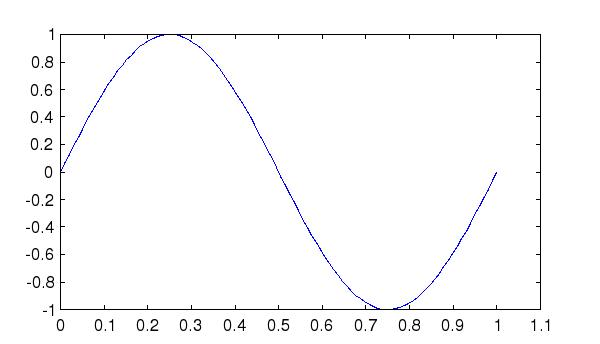
\includegraphics[width=8cm]{sinplot}}


\section{SIND Sine Degrees Function}

\subsection{Usage}

Computes the sine of the argument, but takes
the argument in degrees instead of radians (as is the case
for \verb|cos|). The syntax for its use is
\begin{verbatim}
   y = sind(x)
\end{verbatim}
\subsection{Examples}

The sine of 45 degrees should be \verb|sqrt(2)/2|
\begin{verbatim}
--> sind(45)

ans = 

    0.7071 
\end{verbatim}
and the sine of \verb|30| degrees should be 0.5:
\begin{verbatim}
--> sind(30)

ans = 

    0.5000 
\end{verbatim}

\section{SINH Hyperbolic Sine Function}

\subsection{Usage}

Computes the hyperbolic sine of the argument.
The syntax for its use is
\begin{verbatim}
   y = sinh(x)
\end{verbatim}
\subsection{Function Internals}

The \verb|sinh| function is computed from the formula
\[
   \sinh(x) = \frac{e^x-e^{-x}}{2}
\]
\subsection{Examples}

Here is a simple plot of the hyperbolic sine function
\begin{verbatim}
--> x = linspace(-5,5);
--> plot(x,sinh(x)); grid('on');
\end{verbatim}


\centerline{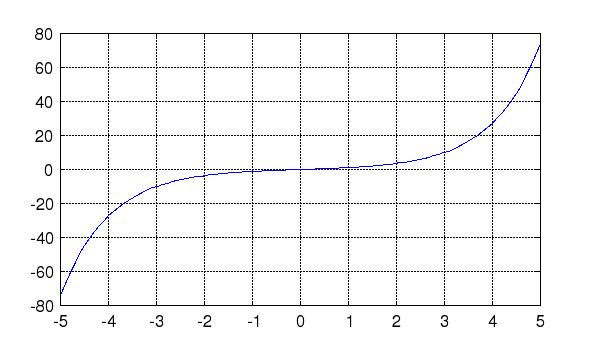
\includegraphics[width=8cm]{sinhplot}}


\section{SQRT Square Root of an Array}

\subsection{Usage}

Computes the square root of the argument matrix.  The general
syntax for its use is
\begin{verbatim}
   y = sqrt(x)
\end{verbatim}
where \verb|x| is an N-dimensional numerical array.
\subsection{Example}

Here are some examples of using \verb|sqrt|
\begin{verbatim}
--> sqrt(9)

ans = 
 3 

--> sqrt(i)

ans = 
   0.7071 +  0.7071i 

--> sqrt(-1)

ans = 
   0.0000 +  1.0000i 

--> x = rand(4)

x = 
    0.6031    0.7537    0.6479    0.3985 
    0.8219    0.3124    0.3073    0.5023 
    0.1780    0.9026    0.5598    0.9462 
    0.6403    0.4911    0.4890    0.7665 

--> sqrt(x)

ans = 
    0.7766    0.8681    0.8049    0.6313 
    0.9066    0.5589    0.5543    0.7087 
    0.4219    0.9501    0.7482    0.9727 
    0.8002    0.7008    0.6993    0.8755 
\end{verbatim}

\section{TAN Trigonometric Tangent Function}

\subsection{Usage}

Computes the \verb|tan| function for its argument.  The general
syntax for its use is
\begin{verbatim}
  y = tan(x)
\end{verbatim}
where \verb|x| is an \verb|n|-dimensional array of numerical type.
Integer types are promoted to the \verb|double| type prior to
calculation of the \verb|tan| function.  Output \verb|y| is of the
same size and type as the input \verb|x|, (unless \verb|x| is an
integer, in which case \verb|y| is a \verb|double| type).  
\subsection{Function Internals}

Mathematically, the \verb|tan| function is defined for all real
valued arguments \verb|x| by the infinite summation
\[
  \tan x \equiv x + \frac{x^3}{3} + \frac{2x^5}{15} + \cdots,
\]
or alternately by the ratio
\[
  \tan x \equiv \frac{\sin x}{\cos x}
\]
For complex valued arguments \verb|z|, the tangent is computed via
\[
  \tan z \equiv \frac{\sin 2 \Re z + i \sinh 2 \Im z}
                     {\cos 2 \Re z + \cosh 2 \Im z}.
\]
\subsection{Example}

The following piece of code plots the real-valued \verb|tan(x)|
function over the interval \verb|[-1,1]|:
\begin{verbatim}
--> t = linspace(-1,1);
--> plot(t,tan(t))
\end{verbatim}


\centerline{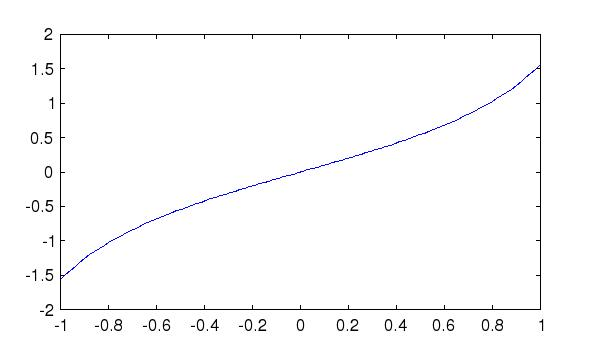
\includegraphics[width=8cm]{tanplot}}


\section{TAND Tangent Degrees Function}

\subsection{Usage}

Computes the tangent of the argument, but takes
the argument in degrees instead of radians (as is the case
for \verb|cos|). The syntax for its use is
\begin{verbatim}
   y = tand(x)
\end{verbatim}
\subsection{Examples}

The tangent of 45 degrees should be \verb|1|
\begin{verbatim}
--> tand(45)

ans = 

    1.0000 
\end{verbatim}

\section{TANH Hyperbolic Tangent Function}

\subsection{Usage}

Computes the hyperbolic tangent of the argument.
The syntax for its use is
\begin{verbatim}
   y = tanh(x)
\end{verbatim}
\subsection{Function Internals}

The \verb|tanh| function is computed from the formula
\[
   \tanh(x) = \frac{\sinh(x)}{\cosh(x)}
\]
\subsection{Examples}

Here is a simple plot of the hyperbolic tangent function
@>


\centerline{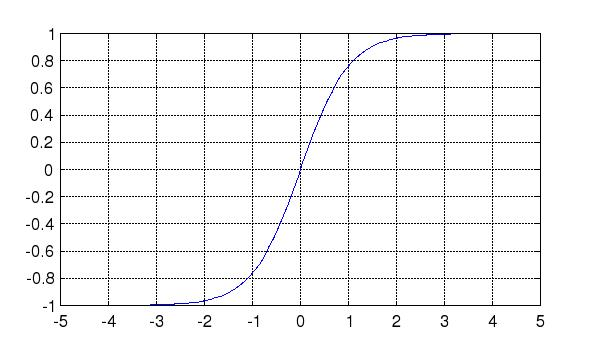
\includegraphics[width=8cm]{tanhplot}}


\chapter{Base Constants}
\section{E Euler Constant (Base of Natural Logarithm)}

\subsection{Usage}

Returns a \verb|double| (64-bit floating point number) value that represents Euler's constant, the base of the natural logarithm.  Typical usage 
\begin{verbatim}
   y = e
\end{verbatim}
This value is approximately 2.718281828459045.
\subsection{Example}

The following example demonstrates the use of the \verb|e| function.
\begin{verbatim}
--> e

ans = 

    2.7183 

--> log(e)

ans = 

 1 
\end{verbatim}

\section{EPS Double Precision Floating Point Relative Machine Precision Epsilon}

\subsection{Usage}

Returns \verb|eps|, which quantifies the relative machine precision
of floating point numbers (a machine specific quantity).  The syntax
for \verb|eps| is:
\begin{verbatim}
   y = eps
   y = eps('double')
   y = eps(X)
\end{verbatim}
First form returns \verb|eps| for \verb|double| precision values. For most
typical processors, this value is approximately \verb|2^-52|, or 2.2204e-16.
Second form return \verb|eps| for class \verb|double| or \verb|single|.
Third form returns distance to the next value greater than X.
\subsection{Example}

The following example demonstrates the use of the \verb|eps| function,
and one of its numerical consequences.
\begin{verbatim}
--> eps

ans = 

 2.2204e-16 

--> 1.0+eps

ans = 

    1.0000 

--> eps(1000.)

ans = 

 1.1369e-13 
\end{verbatim}

\section{FALSE Logical False}

\subsection{Usage}

Returns a logical 0.  The syntax for its use is
\begin{verbatim}
   y = false
\end{verbatim}

\section{FEPS Single Precision Floating Point Relative Machine Precision Epsilon}

\subsection{Usage}

Returns \verb|feps|, which quantifies the relative machine precision
of floating point numbers (a machine specific quantity).  The syntax
for \verb|feps| is:
\begin{verbatim}
   y = feps
\end{verbatim}
which returns \verb|feps| for \verb|single| precision values. For most
typical processors, this value is approximately \verb|2^-24|, or 5.9604e-8.
\subsection{Example}

The following example demonstrates the use of the \verb|feps| function,
and one of its numerical consequences.
\begin{verbatim}
--> feps

ans = 
 1.1921e-07 

--> 1.0f+eps

ans = 
 1 
\end{verbatim}

\section{I-J Square Root of Negative One}

\subsection{Usage}

Returns a \verb|complex| value that represents the square root of -1.  There are two
functions that return the same value:
\begin{verbatim}
   y = i
\end{verbatim}
and 
\begin{verbatim}
   y = j.
\end{verbatim}
This allows either \verb|i| or \verb|j| to be used as loop indices.  The returned value is a 32-bit complex value.
\subsection{Example}

The following examples demonstrate a few calculations with \verb|i|.
@>
The same calculations with \verb|j|:
@>
Here is an example of how \verb|i| can be used as a loop index and then recovered as the square root of -1.
@>

\section{INF Infinity Constant}

\subsection{Usage}

Returns a value that represents positive infinity 
for both 32 and 64-bit floating point values. 
There are several forms for the \verb|Inf| function.
The first form returns a double precision \verb|Inf|.
\begin{verbatim}
   y = inf
\end{verbatim}
The next form takes a class name that can be either \verb|'double'| 
\begin{verbatim}
   y = inf('double')
\end{verbatim}
or \verb|'single'|:
\begin{verbatim}
   y = inf('single')
\end{verbatim}
With a single parameter it generates a square matrix of \verb|inf|s.
\begin{verbatim}
   y = inf(n)
\end{verbatim}
Alternatively, you can specify the dimensions of the array via
\begin{verbatim}
   y = inf(m,n,p,...)
\end{verbatim}
or
\begin{verbatim}
   y = inf([m,n,p,...])
\end{verbatim}
Finally, you can add a classname of either \verb|'single'| or \verb|'double'|.
\subsection{Function Internals}

The infinity constant has
several interesting properties.  In particular:
\[
\begin{array}{ll}
   \infty \times 0 & = \mathrm{NaN} \\                                             \infty \times a & = \infty \, \mathrm{for all} \, a > 0 \\   \infty \times a & = -\infty \, \mathrm{for all} \, a < 0 \\   \infty / \infty & = \mathrm{NaN} \\   \infty / 0 & = \infty 
\end{array}
\]
Note that infinities are not preserved under type conversion to integer types (see the examples below).
\subsection{Example}

The following examples demonstrate the various properties of the infinity constant.
@>
Note that infinities are preserved under type conversion to floating point types (i.e., \verb|float|, \verb|double|, \verb|complex| and \verb|dcomplex| types), but not integer  types.
@>

\section{PI Constant Pi}

\subsection{Usage}

Returns a \verb|double| (64-bit floating point number) value that represents pi (ratio between the circumference and diameter of a circle...).  Typical usage 
\begin{verbatim}
   y = pi
\end{verbatim}
This value is approximately 3.141592653589793.
\subsection{Example}

The following example demonstrates the use of the \verb|pi| function.
@>

\section{TEPS Type-based Epsilon Calculation}

\subsection{Usage}

Returns \verb|eps| for double precision arguments and
\verb|feps| for single precision arguments.  The syntax for
\verb|teps| is
\begin{verbatim}
   y = teps(x)
\end{verbatim}
The \verb|teps| function is most useful if you need to
compute epsilon based on the type of the array.
\subsection{Example}

The following example demonstrates the use of the \verb|teps| function,
and one of its numerical consequences.
@>

\section{TRUE Logical TRUE}

\subsection{Usage}

Returns a logical 1.  The syntax for its use is
\begin{verbatim}
   y = true
\end{verbatim}
You can also create an array of logical ones using
the syntax
\begin{verbatim}
   y = true(d1,d2,...,dn)
\end{verbatim}
or the syntax
\begin{verbatim}
   y = true([d1,d2,...,dn])
\end{verbatim}

\chapter{Elementary Functions}
\section{ABS Absolute Value Function}

\subsection{Usage}

Returns the absolute value of the input array for all elements.  The 
general syntax for its use is
\begin{verbatim}
   y = abs(x)
\end{verbatim}
where \verb|x| is an \verb|n|-dimensional array of numerical type.  The output 
is the same numerical type as the input, unless the input is \verb|complex|
or \verb|dcomplex|.  For \verb|complex| inputs, the absolute value is a floating
point array, so that the return type is \verb|float|.  For \verb|dcomplex|
inputs, the absolute value is a double precision floating point array, so that
the return type is \verb|double|.
\subsection{Example}

The following demonstrates the \verb|abs| applied to a complex scalar.
@>
The \verb|abs| function applied to integer and real values:
@>
For a double-precision complex array,
@>

\section{ALL All True Function}

\subsection{Usage}

Reduces a logical array along a given dimension by testing for all
logical 1s.  The general 
syntax for its use is
\begin{verbatim}
  y = all(x,d)
\end{verbatim}
where \verb|x| is an \verb|n|-dimensions array of \verb|logical| type.
The output is of \verb|logical| type.  The argument \verb|d| is 
optional, and denotes the dimension along which to operate.
The output \verb|y| is the same size as \verb|x|, except that it is 
singular along the operated direction.  So, for example,
if \verb|x| is a \verb|3 x 3 x 4| array, and we \verb|all| operation along
dimension \verb|d=2|, then the output is of size \verb|3 x 1 x 4|.
\subsection{Function Internals}

The output is computed via
\[
y(m_1,\ldots,m_{d-1},1,m_{d+1},\ldots,m_{p}) = 
\min_{k} x(m_1,\ldots,m_{d-1},k,m_{d+1},\ldots,m_{p})
\]
If \verb|d| is omitted, then the minimum is taken over all elements of
\verb|x|.
\subsection{Example}

The following piece of code demonstrates various uses of the \verb|all|
function
\begin{verbatim}
--> A = [1,0,0;1,0,0;0,0,1]

A = 

 1 0 0 
 1 0 0 
 0 0 1 
\end{verbatim}
We start by calling \verb|all| without a dimension argument, in which 
case it defaults to testing all values of \verb|A|
\begin{verbatim}
--> all(A)

ans = 

 0 0 0 
\end{verbatim}
The \verb|all| function is useful in expressions also.
\begin{verbatim}
--> all(A>=0)

ans = 

 1 1 1 
\end{verbatim}
Next, we apply the \verb|all| operation along the rows.
\begin{verbatim}
--> all(A,2)

ans = 

 0 
 0 
 0 
\end{verbatim}

\section{ANY Any True Function}

\subsection{Usage}

Reduces a logical array along a given dimension by testing for any
logical 1s.  The general 
syntax for its use is
\begin{verbatim}
  y = any(x,d)
\end{verbatim}
where \verb|x| is an \verb|n|-dimensions array of \verb|logical| type.
The output is of \verb|logical| type.  The argument \verb|d| is 
optional, and denotes the dimension along which to operate.
The output \verb|y| is the same size as \verb|x|, except that it is 
singular along the operated direction.  So, for example,
if \verb|x| is a \verb|3 x 3 x 4| array, and we \verb|any| operation along
dimension \verb|d=2|, then the output is of size \verb|3 x 1 x 4|.
\subsection{Function Internals}

The output is computed via
\[
y(m_1,\ldots,m_{d-1},1,m_{d+1},\ldots,m_{p}) = 
\max_{k} x(m_1,\ldots,m_{d-1},k,m_{d+1},\ldots,m_{p})
\]
If \verb|d| is omitted, then the summation is taken along the 
first non-singleton dimension of \verb|x|. 
\subsection{Example}

The following piece of code demonstrates various uses of the summation
function
@>
We start by calling \verb|any| without a dimension argument, in which 
case it defaults to the first nonsingular dimension (in this case, 
along the columns or \verb|d = 1|).
@>
Next, we apply the \verb|any| operation along the rows.
@>

\section{CEIL Ceiling Function}

\subsection{Usage}

Computes the ceiling of an n-dimensional array elementwise.  The
ceiling of a number is defined as the smallest integer that is
larger than or equal to that number. The general syntax for its use
is
\begin{verbatim}
   y = ceil(x)
\end{verbatim}
where \verb|x| is a multidimensional array of numerical type.  The \verb|ceil| 
function preserves the type of the argument.  So integer arguments 
are not modified, and \verb|float| arrays return \verb|float| arrays as 
outputs, and similarly for \verb|double| arrays.  The \verb|ceil| function 
is not defined for \verb|complex| or \verb|dcomplex| types.
\subsection{Example}

The following demonstrates the \verb|ceil| function applied to various
(numerical) arguments.  For integer arguments, the ceil function has
no effect:
\begin{verbatim}
--> ceil(3)

ans = 

 3 

--> ceil(-3)

ans = 

 -3 
\end{verbatim}
Next, we take the \verb|ceil| of a floating point value:
\begin{verbatim}
--> ceil(float(3.023))

ans = 

 4 

--> ceil(float(-2.341))

ans = 

 -2 
\end{verbatim}
Note that the return type is a \verb|float| also.  Finally, for a \verb|double|
type:
\begin{verbatim}
--> ceil(4.312)

ans = 

 5 

--> ceil(-5.32)

ans = 

 -5 
\end{verbatim}

\section{CONJ Conjugate Function}

\subsection{Usage}

Returns the complex conjugate of the input array for all elements.  The 
general syntax for its use is
\begin{verbatim}
   y = conj(x)
\end{verbatim}
where \verb|x| is an \verb|n|-dimensional array of numerical type.  The output 
is the same numerical type as the input.  The \verb|conj| function does
nothing to real and integer types.
\subsection{Example}

The following demonstrates the complex conjugate applied to a complex scalar.
@>
The \verb|conj| function has no effect on real arguments:
@>
For a double-precision complex array,
@>

\section{CUMPROD Cumulative Product Function}

\subsection{Usage}

Computes the cumulative product of an n-dimensional array along a given
dimension.  The general syntax for its use is
\begin{verbatim}
  y = cumprod(x,d)
\end{verbatim}
where \verb|x| is a multidimensional array of numerical type, and \verb|d|
is the dimension along which to perform the cumulative product.  The
output \verb|y| is the same size of \verb|x|.  Integer types are promoted
to \verb|int32|. If the dimension \verb|d| is not specified, then the
cumulative sum is applied along the first non-singular dimension.
\subsection{Function Internals}

The output is computed via
\[
  y(m_1,\ldots,m_{d-1},j,m_{d+1},\ldots,m_{p}) = 
  \prod_{k=1}^{j} x(m_1,\ldots,m_{d-1},k,m_{d+1},\ldots,m_{p}).
\]
\subsection{Example}

The default action is to perform the cumulative product along the
first non-singular dimension.
@>
To compute the cumulative product along the columns:
@>
The cumulative product also works along arbitrary dimensions
@>

\section{CUMSUM Cumulative Summation Function}

\subsection{Usage}

Computes the cumulative sum of an n-dimensional array along a given
dimension.  The general syntax for its use is
\begin{verbatim}
  y = cumsum(x,d)
\end{verbatim}
where \verb|x| is a multidimensional array of numerical type, and \verb|d|
is the dimension along which to perform the cumulative sum.  The
output \verb|y| is the same size of \verb|x|.  Integer types are promoted
to \verb|int32|. If the dimension \verb|d| is not specified, then the
cumulative sum is applied along the first non-singular dimension.
\subsection{Function Internals}

The output is computed via
\[
  y(m_1,\ldots,m_{d-1},j,m_{d+1},\ldots,m_{p}) = 
  \sum_{k=1}^{j} x(m_1,\ldots,m_{d-1},k,m_{d+1},\ldots,m_{p}).
\]
\subsection{Example}

The default action is to perform the cumulative sum along the
first non-singular dimension.
@>
To compute the cumulative sum along the columns:
@>
The cumulative sum also works along arbitrary dimensions
@>

\section{DEAL Multiple Simultaneous Assignments}

\subsection{Usage}

When making a function call, it is possible to assign
multiple outputs in a single call, (see, e.g., \verb|max| for
an example).  The \verb|deal| call allows you to do the 
same thing with a simple assignment.  The syntax for its
use is
\begin{verbatim}
   [a,b,c,...] = deal(expr)
\end{verbatim}
where \verb|expr| is an expression with multiple values.  The simplest
example is where \verb|expr| is the dereference of a cell array, e.g.
\verb|expr <-- A{:}|.  In this case, the \verb|deal| call is equivalent
to
\begin{verbatim}
   a = A{1}; b = A{2}; C = A{3}; 
\end{verbatim}
Other expressions which are multivalued are structure arrays with
multiple entries (non-scalar), where field dereferencing has been
applied.

\section{DEC2HEX Convert Decimal Number to Hexadecimal}

\subsection{Usage}

Converts an integer value into its hexadecimal representation.  The syntax
for its use is
\begin{verbatim}
   y = dec2hex(x)
\end{verbatim}
where \verb|x| is an integer (and is promoted to a 64-bit integer if it is not).
The returned value \verb|y| is a string containing the hexadecimal representation
of that integer.  If you require a minimum length for the hexadecimal
representation, you can specify an optional second argument
\begin{verbatim}
   y = dec2hex(x,n)
\end{verbatim}
where \verb|n| indicates the minimum number of digits in the representation.
\subsection{Example}

Here are some simple examples:
\begin{verbatim}
--> dec2hex(1023)

ans = 

 3FF
\end{verbatim}
\begin{verbatim}
--> dec2hex(58128493)

ans = 

 376F86D
\end{verbatim}

\section{DIFF Difference Function}

\subsection{Usage}

\begin{verbatim}
	y=diff(x)
	y=diff(x,k)
	y=diff(x,k,dim)
\end{verbatim}
 Produce difference of successive vector elements.
 
 If \verb|x| is a vector of length n, \verb|diff (x)| is the
 vector of first differences
 \[
  [x_2 - x_1, ..., x_n - x_{n-1}].
 \]

 If \verb|x| is a matrix, \verb|diff (x)| is the matrix of column
 differences along the first non-singleton dimension.

 The second argument is optional.  If supplied, \verb|diff (x,k)|,
 where \verb|k| is a nonnegative integer, returns the
 \verb|k|-th differences. It is possible that \verb|k| is larger than
 then first non-singleton dimension of the matrix. In this case,
 \verb|diff| continues to take the differences along the next
 non-singleton dimension.

 The dimension along which to take the difference can be explicitly
 stated with the optional variable \verb|dim|. In this case the 
 \verb|k|-th order differences are calculated along this dimension.
 In the case where \verb|k| exceeds \verb|size (x, dim)|
 then an empty matrix is returned.


\section{DOT Dot Product Function}

\subsection{Usage}

Computes the scalar dot product of its two arguments.  The general
syntax for its use is
\begin{verbatim}
  y = dot(x,z)
\end{verbatim}
where \verb|x| and \verb|z| are numerical vectors of the same length.  If 
\verb|x| and \verb|z| are multi-dimensional arrays of the same size, then
the dot product is taken along the first non-singleton dimension.
You can also specify the dimension to take the dot product along using
the alternate form
\begin{verbatim}
  y = dot(x,z,dim)
\end{verbatim}
where \verb|dim| specifies the dimension to take the dot product along.

\section{FLOOR Floor Function}

\subsection{Usage}

Computes the floor of an n-dimensional array elementwise.  The
floor of a number is defined as the smallest integer that is
less than or equal to that number. The general syntax for its use
is
\begin{verbatim}
   y = floor(x)
\end{verbatim}
where \verb|x| is a multidimensional array of numerical type.  The \verb|floor| 
function preserves the type of the argument.  So integer arguments 
are not modified, and \verb|float| arrays return \verb|float| arrays as 
outputs, and similarly for \verb|double| arrays.  The \verb|floor| function 
is not defined for complex types.
\subsection{Example}

The following demonstrates the \verb|floor| function applied to various
(numerical) arguments.  For integer arguments, the floor function has
no effect:
@>
Next, we take the \verb|floor| of a floating point value:
@>

\section{GETFIELD Get Field Contents}

\subsection{Usage}

Given a structure or structure array, returns the contents of the
specified field.  The first version is for scalar structures, and
has the following syntax
\begin{verbatim}
   y = getfield(x,'fieldname')
\end{verbatim}
and is equivalent to \verb|y = x.fieldname| where \verb|x| is a scalar (1 x 1)
structure.  If \verb|x| is not a scalar structure, then \verb|y| is the 
first value, i.e., it is equivalent to \verb|y = x(1).fieldname|.  
The second form allows you to specify a subindex into a
structure array, and has the following syntax
\begin{verbatim}
    y = getfield(x, {m,n}, 'fieldname')
\end{verbatim}
and is equivalent to \verb|y = x(m,n).fieldname|.  You can chain multiple
references together using this syntax.

\section{HEX2DEC Convert Hexadecimal Numbers To Decimal}

\subsection{Usage}

Converts a hexadecimal number (encoded as a string matrix) into integers.
The syntax for its use is
\begin{verbatim}
   y = hex2dec(x)
\end{verbatim}
where \verb|x| is a character matrix where each row represents an integer
in hexadecimal form.  The output is of type \verb|FM_DOUBLE|.
\subsection{Examples}

\begin{verbatim}
--> hex2dec('3ff')

ans = 

 1023 
\end{verbatim}
Or for a more complex example
\begin{verbatim}
--> hex2dec(['0ff';'2de';'123'])

ans = 

 255 
 734 
 291 
\end{verbatim}

\section{IMAG Imaginary Function}

\subsection{Usage}

Returns the imaginary part of the input array for all elements.  The 
general syntax for its use is
\begin{verbatim}
   y = imag(x)
\end{verbatim}
where \verb|x| is an \verb|n|-dimensional array of numerical type.  The output 
is the same numerical type as the input, unless the input is \verb|complex|
or \verb|dcomplex|.  For \verb|complex| inputs, the imaginary part is a floating
point array, so that the return type is \verb|float|.  For \verb|dcomplex|
inputs, the imaginary part is a double precision floating point array, so that
the return type is \verb|double|.  The \verb|imag| function returns zeros for 
real and integer types.
\subsection{Example}

The following demonstrates \verb|imag| applied to a complex scalar.
@>
The imaginary part of real and integer arguments is a vector of zeros, the
same type and size of the argument.
@>
For a double-precision complex array,
@>

\section{MAX Maximum Function}

\subsection{Usage}

Computes the maximum of an array along a given dimension, or alternately, 
computes two arrays (entry-wise) and keeps the smaller value for each array.
As a result, the \verb|max| function has a number of syntaxes.  The first
one computes the maximum of an array along a given dimension.
The first general syntax for its use is either
\begin{verbatim}
   [y,n] = max(x,[],d)
\end{verbatim}
where \verb|x| is a multidimensional array of numerical type, in which case the
output \verb|y| is the maximum of \verb|x| along dimension \verb|d|.  
The second argument \verb|n| is the index that results in the maximum.
In the event that multiple maxima are present with the same value,
the index of the first maximum is used. 
The second general syntax for the use of the \verb|max| function is
\begin{verbatim}
   [y,n] = max(x)
\end{verbatim}
In this case, the maximum is taken along the first non-singleton 
dimension of \verb|x|.  For complex data types,
the maximum is based on the magnitude of the numbers.  NaNs are
ignored in the calculations.
The third general syntax for the use of the \verb|max| function is as 
a comparison function for pairs of arrays.  Here, the general syntax is
\begin{verbatim}
   y = max(x,z)
\end{verbatim}
where \verb|x| and \verb|z| are either both numerical arrays of the same dimensions,
or one of the two is a scalar.  In the first case, the output is the 
same size as both arrays, and is defined elementwise by the smaller of the
two arrays.  In the second case, the output is defined elementwise by the 
smaller of the array entries and the scalar.
\subsection{Function Internals}

In the general version of the \verb|max| function which is applied to
a single array (using the \verb|max(x,[],d)| or \verb|max(x)| syntaxes),
The output is computed via
\[
y(m_1,\ldots,m_{d-1},1,m_{d+1},\ldots,m_{p}) = 
\max_{k} x(m_1,\ldots,m_{d-1},k,m_{d+1},\ldots,m_{p}),
\]
and the output array \verb|n| of indices is calculated via
\[
n(m_1,\ldots,m_{d-1},1,m_{d+1},\ldots,m_{p}) = \arg
\max_{k} x(m_1,\ldots,m_{d-1},k,m_{d+1},\ldots,m_{p})
\]
In the two-array version (\verb|max(x,z)|), the single output is computed as
\[
  y(m_1,\ldots,m_{d-1},1,m_{d+1},\ldots,m_{p}) = 
\begin{cases}
  x(m_1,\ldots,m_{d-1},k,m_{d+1},\ldots,m_{p}) & x(\cdots) \leq z(\cdots) \\    z(m_1,\ldots,m_{d-1},k,m_{d+1},\ldots,m_{p}) & z(\cdots) < x(\cdots).
\end{cases}
\]
\subsection{Example}

The following piece of code demonstrates various uses of the maximum
function.  We start with the one-array version.
@>
We first take the maximum along the columns, resulting in a row vector.
@>
Next, we take the maximum along the rows, resulting in a column vector.
@>
When the dimension argument is not supplied, \verb|max| acts along the first non-singular dimension.  For a row vector, this is the column direction:
@>

For the two-argument version, we can compute the smaller of two arrays,
as in this example:
@>
Or alternately, we can compare an array with a scalar
@>

\section{MEAN Mean Function}

\subsection{Usage}

Computes the mean of an array along a given dimension.  The general
syntax for its use is
\begin{verbatim}
  y = mean(x,d)
\end{verbatim}
where \verb|x| is an \verb|n|-dimensions array of numerical type.
The output is of the same numerical type as the input.  The argument
\verb|d| is optional, and denotes the dimension along which to take
the mean.  The output \verb|y| is the same size as \verb|x|, except
that it is singular along the mean direction.  So, for example,
if \verb|x| is a \verb|3 x 3 x 4| array, and we compute the mean along
dimension \verb|d=2|, then the output is of size \verb|3 x 1 x 4|.
\subsection{Function Internals}

The output is computed via
\[
y(m_1,\ldots,m_{d-1},1,m_{d+1},\ldots,m_{p}) = \frac{1}{N}
\sum_{k=1}^{N} x(m_1,\ldots,m_{d-1},k,m_{d+1},\ldots,m_{p})
\]
If \verb|d| is omitted, then the mean is taken along the 
first non-singleton dimension of \verb|x|. 
\subsection{Example}

The following piece of code demonstrates various uses of the mean
function
\begin{verbatim}
--> A = [5,1,3;3,2,1;0,3,1]

A = 
 5 1 3 
 3 2 1 
 0 3 1 
\end{verbatim}
We start by calling \verb|mean| without a dimension argument, in which 
case it defaults to the first nonsingular dimension (in this case, 
along the columns or \verb|d = 1|).
\begin{verbatim}
--> mean(A)

ans = 
    2.6667    2.0000    1.6667 
\end{verbatim}
Next, we take the mean along the rows.
\begin{verbatim}
--> mean(A,2)

ans = 
    3.0000 
    2.0000 
    1.3333 
\end{verbatim}

\section{MIN Minimum Function}

\subsection{Usage}

Computes the minimum of an array along a given dimension, or alternately, 
computes two arrays (entry-wise) and keeps the smaller value for each array.
As a result, the \verb|min| function has a number of syntaxes.  The first
one computes the minimum of an array along a given dimension.
The first general syntax for its use is either
\begin{verbatim}
   [y,n] = min(x,[],d)
\end{verbatim}
where \verb|x| is a multidimensional array of numerical type, in which case the
output \verb|y| is the minimum of \verb|x| along dimension \verb|d|.  
The second argument \verb|n| is the index that results in the minimum.
In the event that multiple minima are present with the same value,
the index of the first minimum is used. 
The second general syntax for the use of the \verb|min| function is
\begin{verbatim}
   [y,n] = min(x)
\end{verbatim}
In this case, the minimum is taken along the first non-singleton 
dimension of \verb|x|.  For complex data types,
the minimum is based on the magnitude of the numbers.  NaNs are
ignored in the calculations.
The third general syntax for the use of the \verb|min| function is as 
a comparison function for pairs of arrays.  Here, the general syntax is
\begin{verbatim}
   y = min(x,z)
\end{verbatim}
where \verb|x| and \verb|z| are either both numerical arrays of the same dimensions,
or one of the two is a scalar.  In the first case, the output is the 
same size as both arrays, and is defined elementwise by the smaller of the
two arrays.  In the second case, the output is defined elementwise by the 
smaller of the array entries and the scalar.
\subsection{Function Internals}

In the general version of the \verb|min| function which is applied to
a single array (using the \verb|min(x,[],d)| or \verb|min(x)| syntaxes),
The output is computed via
\[
y(m_1,\ldots,m_{d-1},1,m_{d+1},\ldots,m_{p}) = 
\min_{k} x(m_1,\ldots,m_{d-1},k,m_{d+1},\ldots,m_{p}),
\]
and the output array \verb|n| of indices is calculated via
\[
n(m_1,\ldots,m_{d-1},1,m_{d+1},\ldots,m_{p}) = \arg
\min_{k} x(m_1,\ldots,m_{d-1},k,m_{d+1},\ldots,m_{p})
\]
In the two-array version (\verb|min(x,z)|), the single output is computed as
\[
  y(m_1,\ldots,m_{d-1},1,m_{d+1},\ldots,m_{p}) = 
\begin{cases}
  x(m_1,\ldots,m_{d-1},k,m_{d+1},\ldots,m_{p}) & x(\cdots) \leq z(\cdots) \\   z(m_1,\ldots,m_{d-1},k,m_{d+1},\ldots,m_{p}) & z(\cdots) < x(\cdots).
\end{cases}
\]
\subsection{Example}

The following piece of code demonstrates various uses of the minimum
function.  We start with the one-array version.
\begin{verbatim}
--> A = [5,1,3;3,2,1;0,3,1]

A = 
 5 1 3 
 3 2 1 
 0 3 1 
\end{verbatim}
We first take the minimum along the columns, resulting in a row vector.
\begin{verbatim}
--> min(A)

ans = 
 0 1 1 
\end{verbatim}
Next, we take the minimum along the rows, resulting in a column vector.
\begin{verbatim}
--> min(A,[],2)

ans = 
 1 
 1 
 0 
\end{verbatim}
When the dimension argument is not supplied, \verb|min| acts along the first 
non-singular dimension.  For a row vector, this is the column direction:
\begin{verbatim}
--> min([5,3,2,9])

ans = 
 2 
\end{verbatim}

For the two-argument version, we can compute the smaller of two arrays,
as in this example:
\begin{verbatim}
--> a = int8(100*randn(4))

a = 
  -66  -74  -74   32 
 -128  -14 -110 -128 
  127  -96  -49   72 
  127   50   83  120 

--> b = int8(100*randn(4))

b = 
  -94  108  -99  -35 
  127   50 -100  113 
  -98  -39 -127 -107 
  -12  127  103  -44 

--> min(a,b)

ans = 
  -94  -74  -99  -35 
 -128  -14 -110 -128 
  -98  -96 -127 -107 
  -12   50   83  -44 
\end{verbatim}
Or alternately, we can compare an array with a scalar
\begin{verbatim}
--> a = randn(2)

a = 
    0.7713    0.6716 
   -1.0581   -1.3734 

--> min(a,0)

ans = 
         0         0 
   -1.0581   -1.3734 
\end{verbatim}

\section{NUM2HEX Convert Numbers to IEEE Hex Strings}

\subsection{Usage}

Converts single and double precision arrays to IEEE hex strings.  The
syntax for its use is
\begin{verbatim}
   y = num2hex(x)
\end{verbatim}
where \verb|x| is either a \verb|float| or \verb|double| array.  The output \verb|y| is
a \verb|n-by-p| character array, where \verb|n| is the number of elements in \verb|x|,
and \verb|p| is 16 for \verb|double| arrays, and 8 for \verb|single| arrays.
\subsection{Example}

Some interesting numbers
@>
The same in single precision
@>

\section{PROD Product Function}

\subsection{Usage}

Computes the product of an array along a given dimension.  The general
syntax for its use is
\begin{verbatim}
   y = prod(x,d)
\end{verbatim}
where \verb|x| is an \verb|n|-dimensions array of numerical type.
The output is of the same numerical type as the input, except 
for integer types, which are automatically promoted to \verb|int32|.
 The argument \verb|d| is optional, and denotes the dimension along 
which to take the product.  The output is computed via
\[
  y(m_1,\ldots,m_{d-1},1,m_{d+1},\ldots,m_{p}) = 
    \prod_{k} x(m_1,\ldots,m_{d-1},k,m_{d+1},\ldots,m_{p})
\]
If \verb|d| is omitted, then the product is taken along the 
first non-singleton dimension of \verb|x|. Note that by definition
(starting with FreeMat 2.1) \verb|prod([]) = 1|.
\subsection{Example}

The following piece of code demonstrates various uses of the product
function
\begin{verbatim}
--> A = [5,1,3;3,2,1;0,3,1]

A = 
 5 1 3 
 3 2 1 
 0 3 1 
\end{verbatim}
We start by calling \verb|prod| without a dimension argument, in which case it defaults to the first nonsingular dimension (in this case, along the columns or \verb|d = 1|).
\begin{verbatim}
--> prod(A)

ans = 
 0 6 3 
\end{verbatim}
Next, we take the product along the rows.
\begin{verbatim}
--> prod(A,2)

ans = 
 15 
  6 
  0 
\end{verbatim}

\section{REAL Real Function}

\subsection{Usage}

Returns the real part of the input array for all elements.  The 
general syntax for its use is
\begin{verbatim}
   y = real(x)
\end{verbatim}
where \verb|x| is an \verb|n|-dimensional array of numerical type.  The output 
is the same numerical type as the input, unless the input is \verb|complex|
or \verb|dcomplex|.  For \verb|complex| inputs, the real part is a floating
point array, so that the return type is \verb|float|.  For \verb|dcomplex|
inputs, the real part is a double precision floating point array, so that
the return type is \verb|double|.  The \verb|real| function does
nothing to real and integer types.
\subsection{Example}

The following demonstrates the \verb|real| applied to a complex scalar.
\begin{verbatim}
--> real(3+4*i)

ans = 
 3 
\end{verbatim}
The \verb|real| function has no effect on real arguments:
\begin{verbatim}
--> real([2,3,4])

ans = 
 2 3 4 
\end{verbatim}
For a double-precision complex array,
\begin{verbatim}
--> real([2.0+3.0*i,i])

ans = 
 2 0 
\end{verbatim}

\section{ROUND Round Function}

\subsection{Usage}

Rounds an n-dimensional array to the nearest integer elementwise.
The general syntax for its use is
\begin{verbatim}
   y = round(x)
\end{verbatim}
where \verb|x| is a multidimensional array of numerical type.  The \verb|round| 
function preserves the type of the argument.  So integer arguments 
are not modified, and \verb|float| arrays return \verb|float| arrays as 
outputs, and similarly for \verb|double| arrays.  The \verb|round| function 
is not defined for \verb|complex| or \verb|dcomplex| types.
\subsection{Example}

The following demonstrates the \verb|round| function applied to various
(numerical) arguments.  For integer arguments, the round function has
no effect:
\begin{verbatim}
--> round(3)

ans = 

 3 

--> round(-3)

ans = 

 -3 
\end{verbatim}
Next, we take the \verb|round| of a floating point value:
\begin{verbatim}
--> round(3.023f)

ans = 

 3 

--> round(-2.341f)

ans = 

 -2 
\end{verbatim}
Note that the return type is a \verb|float| also.  Finally, for a \verb|double|
type:
\begin{verbatim}
--> round(4.312)

ans = 

 4 

--> round(-5.32)

ans = 

 -5 
\end{verbatim}

\section{STD Standard Deviation Function}

\subsection{Usage}

Computes the standard deviation of an array along a given dimension.  
The general syntax for its use is
\begin{verbatim}
  y = std(x,d)
\end{verbatim}
where \verb|x| is an \verb|n|-dimensions array of numerical type.
The output is of the same numerical type as the input.  The argument
\verb|d| is optional, and denotes the dimension along which to take
the variance.  The output \verb|y| is the same size as \verb|x|, except
that it is singular along the mean direction.  So, for example,
if \verb|x| is a \verb|3 x 3 x 4| array, and we compute the mean along
dimension \verb|d=2|, then the output is of size \verb|3 x 1 x 4|.
\subsection{Example}

The following piece of code demonstrates various uses of the \verb|std|
function
@>
We start by calling \verb|std| without a dimension argument, in which 
case it defaults to the first nonsingular dimension (in this case, 
along the columns or \verb|d = 1|).
@>
Next, we take the variance along the rows.
@>

\section{SUB2IND Convert Multiple Indexing To Linear Indexing}

\subsection{Usage}

The \verb|sub2ind| function converts a multi-dimensional indexing expression
into a linear (or vector) indexing expression.  The syntax for its use
is
\begin{verbatim}
   y = sub2ind(sizevec,d1,d2,...,dn)
\end{verbatim}
where \verb|sizevec| is the size of the array being indexed into, and each
\verb|di| is a vector of the same length, containing index values.  The basic
idea behind \verb|sub2ind| is that it makes
\begin{verbatim}
  [z(d1(1),d2(1),...,dn(1)),...,z(d1(n),d2(n),...,dn(n))]
\end{verbatim}
equivalent to
\begin{verbatim}
  z(sub2ind(size(z),d1,d2,...,dn))
\end{verbatim}
where the later form is using vector indexing, and the former one is using
native, multi-dimensional indexing.
\subsection{Example}

Suppose we have a simple \verb|3 x 4| matrix \verb|A| containing some random integer
elements
\begin{verbatim}
--> A = randi(ones(3,4),10*ones(3,4))

A = 

  2  1  4  2 
  8 10  4  7 
 10  7  4 10 
\end{verbatim}
We can extract the elements \verb|(1,3),(2,3),(3,4)| of \verb|A| via \verb|sub2ind|.
To calculate which elements of \verb|A| this corresponds to, we can use
\verb|sub2ind| as
\begin{verbatim}
--> n = sub2ind(size(A),1:3,2:4)

n = 

  4  8 12 

--> A(n)

ans = 

  1  4 10 
\end{verbatim}

\section{SUM Sum Function}

\subsection{Usage}

Computes the summation of an array along a given dimension.  The general
syntax for its use is
\begin{verbatim}
  y = sum(x,d)
\end{verbatim}
where \verb|x| is an \verb|n|-dimensions array of numerical type.
The output is of the same numerical type as the input.  The argument
\verb|d| is optional, and denotes the dimension along which to take
the summation.  The output \verb|y| is the same size as \verb|x|, except
that it is singular along the summation direction.  So, for example,
if \verb|x| is a \verb|3 x 3 x 4| array, and we compute the summation along
dimension \verb|d=2|, then the output is of size \verb|3 x 1 x 4|.
\subsection{Function Internals}

The output is computed via
\[
y(m_1,\ldots,m_{d-1},1,m_{d+1},\ldots,m_{p}) = 
\sum_{k} x(m_1,\ldots,m_{d-1},k,m_{d+1},\ldots,m_{p})
\]
If \verb|d| is omitted, then the summation is taken along the 
first non-singleton dimension of \verb|x|. 
\subsection{Example}

The following piece of code demonstrates various uses of the summation
function
\begin{verbatim}
--> A = [5,1,3;3,2,1;0,3,1]

A = 

 5 1 3 
 3 2 1 
 0 3 1 
\end{verbatim}
We start by calling \verb|sum| without a dimension argument, in which 
case it defaults to the first nonsingular dimension (in this case, 
along the columns or \verb|d = 1|).
\begin{verbatim}
--> sum(A)

ans = 

 8 6 5 
\end{verbatim}
Next, we take the sum along the rows.
\begin{verbatim}
--> sum(A,2)

ans = 

 9 
 6 
 4 
\end{verbatim}

\section{TEST Test Function}

\subsection{Usage}

Tests for the argument array to be all logical 1s.  It is 
completely equivalent to the \verb|all| function applied to
a vectorized form of the input.  The syntax for the \verb|test|
function is
\begin{verbatim}
   y = test(x)
\end{verbatim}
and the result is equivalent to \verb|all(x(:))|.

\section{VAR Variance Function}

\subsection{Usage}

Computes the variance of an array along a given dimension.  The general
syntax for its use is
\begin{verbatim}
  y = var(x,d)
\end{verbatim}
where \verb|x| is an \verb|n|-dimensions array of numerical type.
The output is of the same numerical type as the input.  The argument
\verb|d| is optional, and denotes the dimension along which to take
the variance.  The output \verb|y| is the same size as \verb|x|, except
that it is singular along the mean direction.  So, for example,
if \verb|x| is a \verb|3 x 3 x 4| array, and we compute the mean along
dimension \verb|d=2|, then the output is of size \verb|3 x 1 x 4|.
\subsection{Function Internals}

The output is computed via
\[
y(m_1,\ldots,m_{d-1},1,m_{d+1},\ldots,m_{p}) = \frac{1}{N-1}
\sum_{k=1}^{N} \left(x(m_1,\ldots,m_{d-1},k,m_{d+1},\ldots,m_{p}) 
 - \bar{x}\right)^2,
\]
where 
\[
\bar{x}  = \frac{1}{N}
\sum_{k=1}^{N} x(m_1,\ldots,m_{d-1},k,m_{d+1},\ldots,m_{p})
\]
If \verb|d| is omitted, then the mean is taken along the 
first non-singleton dimension of \verb|x|. 
\subsection{Example}

The following piece of code demonstrates various uses of the var
function
@>
We start by calling \verb|var| without a dimension argument, in which 
case it defaults to the first nonsingular dimension (in this case, 
along the columns or \verb|d = 1|).
@>
Next, we take the variance along the rows.
@>

\section{VEC Reshape to a Vector}

\subsection{Usage}

Reshapes an n-dimensional array into a column vector.  The general
syntax for its use is
\begin{verbatim}
   y = vec(x)
\end{verbatim}
where \verb|x| is an n-dimensional array (not necessarily numeric).  This
function is equivalent to the expression \verb|y = x(:)|.
\subsection{Example}

A simple example of the \verb|vec| operator reshaping a 2D matrix:
\begin{verbatim}
--> A = [1,2,4,3;2,3,4,5]

A = 
 1 2 4 3 
 2 3 4 5 

--> vec(A)

ans = 
 1 
 2 
 2 
 3 
 4 
 4 
 3 
 5 
\end{verbatim}

\chapter{Inspection Functions}
\section{CLEAR Clear or Delete a Variable}

\subsection{Usage}

Clears a set of variables from the current context, or alternately, 
delete all variables defined in the current context.  There are
several formats for the function call.  The first is the explicit form
in which a list of variables are provided:
\begin{verbatim}
   clear a1 a2 ...
\end{verbatim}
The variables can be persistent or global, and they will be deleted.
The second form
\begin{verbatim}
   clear 'all'
\end{verbatim}
clears all variables and libraries from the current context.  Alternately, you can
use the form:
\begin{verbatim}
   clear 'libs'
\end{verbatim}
which will unload any libraries or DLLs that have been \verb|import|ed. 
Optionally, you can specify that persistent variables should be cleared via:
\begin{verbatim}
   clear 'persistent'
\end{verbatim}
and similarly for global variables:
\begin{verbatim}
   clear 'global'
\end{verbatim}
You can use
\begin{verbatim}
   clear 'classes'
\end{verbatim}
to clear all definitions of user-defined classes.
With no arguments, \verb|clear| defaults to clearing \verb|'all'|.
\subsection{Example}

Here is a simple example of using \verb|clear| to delete a variable.  First, we create a variable called \verb|a|:
\begin{verbatim}
--> a = 53

a = 
 53 
\end{verbatim}
Next, we clear \verb|a| using the \verb|clear| function, and verify that it is deleted.
\begin{verbatim}
--> clear a
--> a
Error: Undefined function or variable a
\end{verbatim}

\section{END End Function}

\subsection{Usage}

Computes the size of a variable along a given dimension.  The syntax
for its use is 
\begin{verbatim}
   y = end(x,dim,subindexes)
\end{verbatim}
where \verb|x| is the array to be analyzed, \verb|dim| is the dimension along
which to compute the end, and \verb|subindexes| indicates how many dimensions
are involved in the \verb|end| calculation.

\section{EXIST Test for Existence}

\subsection{Usage}

Tests for the existence of a variable, function, directory or
file.  The general syntax for its use is
\begin{verbatim}
  y = exist(item,kind)
\end{verbatim}
where \verb|item| is a string containing the name of the item
to look for, and \verb|kind| is a string indicating the type 
of the search.  The \verb|kind| must be one of 
\begin{itemize}
\item  \verb|'builtin'| checks for built-in functions

\item  \verb|'dir'| checks for directories

\item  \verb|'file'| checks for files

\item  \verb|'var'| checks for variables

\item  \verb|'all'| checks all possibilities (same as leaving out \verb|kind|)

\end{itemize}
You can also leave the \verb|kind| specification out, in which case
the calling syntax is
\begin{verbatim}
  y = exist(item)
\end{verbatim}
The return code is one of the following:
\begin{itemize}
\item  0 - if \verb|item| does not exist

\item  1 - if \verb|item| is a variable in the workspace

\item  2 - if \verb|item| is an M file on the search path, a full pathname
 to a file, or an ordinary file on your search path

\item  5 - if \verb|item| is a built-in FreeMat function

\item  7 - if \verb|item| is a directory

\end{itemize}
Note: previous to version \verb|1.10|, \verb|exist| used a different notion
of existence for variables: a variable was said to exist if it 
was defined and non-empty.  This test is now performed by \verb|isset|.
\subsection{Example}

Some examples of the \verb|exist| function.  Note that generally \verb|exist|
is used in functions to test for keywords.  For example,
\begin{verbatim}
  function y = testfunc(a, b, c)
  if (~exist('c'))
    % c was not defined, so establish a default
    c = 13;
  end
  y = a + b + c;
\end{verbatim}
An example of \verb|exist| in action.
\begin{verbatim}
--> a = randn(3,5,2)

a = 

(:,:,1) = 

    0.0744   -0.7000   -1.8022   -0.0255   -0.2933 
   -0.0152   -0.5401   -0.2030   -0.5437    0.9261 
   -0.4359   -1.2334    0.5156    0.0821   -0.5065 

(:,:,2) = 

    0.7408    0.6302   -0.2798    0.7279    1.7674 
    0.9063   -1.7321   -0.8851   -0.4091   -0.5516 
    1.4880    0.5030    0.6747   -0.5492    1.1867 

--> b = []

b = 
  []
--> who
  Variable Name       Type   Flags             Size
              a    double                    [3 5 2]
              b    double                    [0 0]
--> exist('a')

ans = 

 1 

--> exist('b')

ans = 

 1 

--> exist('c')

ans = 

 0 
\end{verbatim}

\section{FIELDNAMES Fieldnames of a Structure}

\subsection{Usage}

Returns a cell array containing the names of the fields in
a structure array.  The syntax for its use is
\begin{verbatim}
   x = fieldnames(y)
\end{verbatim}
where \verb|y| is a structure array of object array.  The result
is a cell array, with one entry per field in \verb|y|.
\subsection{Example}

We define a simple structure array:
@>

\section{ISA Test Type of Variable}

\subsection{Usage}

Tests the type of a variable.  The syntax for its
use is
\begin{verbatim}
   y = isa(x,type)
\end{verbatim}
where \verb|x| is the variable to test, and \verb|type| is
the type.  Supported built-in types are
\begin{itemize}
\item  \verb|'cell'| for cell-arrays

\item  \verb|'struct'| for structure-arrays

\item  \verb|'logical'| for logical arrays

\item  \verb|'uint8'| for unsigned 8-bit integers

\item  \verb|'int8'| for signed 8-bit integers

\item  \verb|'uint16'| for unsigned 16-bit integers

\item  \verb|'int16'| for signed 16-bit integers

\item  \verb|'uint32'| for unsigned 32-bit integers

\item  \verb|'int32'| for signed 32-bit integers

\item  \verb|'uint64'| for unsigned 64-bit integers

\item  \verb|'int64'| for signed 64-bit integers

\item  \verb|'single'| for 32-bit floating point numbers

\item  \verb|'double'| for 64-bit floating point numbers

\item  \verb|'char'| for string arrays

\end{itemize}
If the argument is a user-defined type (via the \verb|class| function), then
the name of that class is returned.
\subsection{Examples}

Here are some examples of the \verb|isa| call.
\begin{verbatim}
--> a = {1}

a = 

 [1] 

--> isa(a,'char')

ans = 

 0 

--> isa(a,'cell')

ans = 

 1 
\end{verbatim}
Here we use \verb|isa| along with shortcut boolean evaluation to 
safely determine if a variable contains the string \verb|'hello'|
\begin{verbatim}
--> a = 'hello'

a = 

 hello

--> isa(a,'char') && strcmp(a,'hello')

ans = 

 1 
\end{verbatim}

\section{ISCELL Test For Cell Array}

\subsection{Usage}

The syntax for \verb|iscell| is 
\begin{verbatim}
   x = iscell(y)
\end{verbatim}
and it returns a logical 1 if the argument is a cell array
and a logical 0 otherwise.
\subsection{Example}

Here are some examples of \verb|iscell|
\begin{verbatim}
--> iscell('foo')

ans = 

 0 

--> iscell(2)

ans = 

 0 

--> iscell({1,2,3})

ans = 

 1 
\end{verbatim}

\section{ISCELLSTR Test For Cell Array of Strings}

\subsection{Usage}

The syntax for \verb|iscellstr| is 
\begin{verbatim}
   x = iscellstr(y)
\end{verbatim}
and it returns a logical 1 if the argument is a cell array
in which every cell is a character array (or is empty), and
a logical 0 otherwise.
\subsection{Example}

Here is a simple example
\begin{verbatim}
--> A = {'Hello','Yellow';'Mellow','Othello'}

A = 
 [Hello] [Yellow] 
 [Mellow] [Othello] 

--> iscellstr(A)

ans = 
 1 
\end{verbatim}

\section{ISCHAR Test For Character Array (string)}

\subsection{Usage}

The syntax for \verb|ischar| is 
\begin{verbatim}
   x = ischar(y)
\end{verbatim}
and it returns a logical 1 if the argument is a string
and a logical 0 otherwise.

\section{ISEMPTY Test For Variable Empty}

\subsection{Usage}

The \verb|isempty| function returns a boolean that indicates
if the argument variable is empty or not.  The general
syntax for its use is
\begin{verbatim}
  y = isempty(x).
\end{verbatim}
\subsection{Examples}

Here are some examples of the \verb|isempty| function
@>
Note that if the variable is not defined, \verb|isempty| 
does not return true.
@>

\section{ISEQUAL Test For Matrix Equality}

\subsection{Usage}

Test two arrays for equality.  The general format
for its use is
\begin{verbatim}
   y = isequal(a,b)
\end{verbatim}
This function returns true if the two arrays are
equal (compared element-wise).  Unlike \verb|issame|
the \verb|isequal| function will type convert where
possible to do the comparison.

\section{ISFIELD Test for Existence of a Structure Field}

\subsection{Usage}

Given a structure array, tests to see if that structure
array contains a field with the given name.  The syntax
for its use is
\begin{verbatim}
  y = isfield(x,field)
\end{verbatim}
and returns a logical \verb|1| if \verb|x| has a field with the 
name \verb|field| and a logical \verb|0| if not.  It also returns
a logical \verb|0| if the argument \verb|x| is not a structure array.
\subsection{Example}

Here we define a simple struct, and then test for some 
fields
\begin{verbatim}
--> a.foo = 32

a = 
    foo: 32
--> a.goo = 64

a = 
    foo: 32
    goo: 64
--> isfield(a,'goo')

ans = 

 1 

--> isfield(a,'got')

ans = 

 0 

--> isfield(pi,'round')

ans = 

 0 
\end{verbatim}

\section{ISHANDLE Test for Graphics Handle}

\subsection{Usage}

Given a constant, this routine will test to see if the
constant is a valid graphics handle or not.  The syntax
for its use is
\begin{verbatim}
  y = ishandle(h,type)
\end{verbatim}
and returns a logical \verb|1| if \verb|x| is a handle of type \verb|type|
and a logical \verb|0| if not.  

\section{ISINF Test for infinities}

\subsection{Usage}

Returns true for entries of an array that are infs (i.e.,
infinities).  The usage is
\begin{verbatim}
   y = isinf(x)
\end{verbatim}
The result is a logical array of the same size as \verb|x|,
which is true if \verb|x| is not-a-number, and false otherwise.
Note that for \verb|complex| or \verb|dcomplex| data types that
the result is true if either the real or imaginary parts
are infinite.
\subsection{Example}

Suppose we have an array of floats with one element that
is \verb|inf|:
\begin{verbatim}
--> a = [1.2 3.4 inf 5]

a = 
    1.2000    3.4000       inf    5.0000 

--> isinf(a)

ans = 
 0 0 1 0 

--> b = 3./[2 5 0 3 1]

b = 
    1.5000    0.6000       inf    1.0000    3.0000 
\end{verbatim}

\section{ISINTTYPE Test For Integer-type Array}

\subsection{Usage}

The syntax for \verb|isinttype| is 
\begin{verbatim}
   x = isinttype(y)
\end{verbatim}
and it returns a logical 1 if the argument is an integer type
and a logical 0 otherwise.  Note that this function only tests
the type of the variable, not the value.  So if, for example,
\verb|y| is a \verb|float| array containing all integer values, it will
still return a logical 0.

\section{ISLOGICAL Test for Logical Array}

\subsection{Usage}

The syntax for \verb|islogical| is 
\begin{verbatim}
   x = islogical(y)
\end{verbatim}
and it returns a logical 1 if the argument is a logical array
and a logical 0 otherwise.

\section{ISMATRIX Test For a 2D Matrix}

\subsection{Usage}

This function tests to see if the argument is a matrix.  The 
syntax for \verb|ismatrix| is
\begin{verbatim}
   x = ismatrix(y)
\end{verbatim}
and it returns a logical 1 if the argument is size \verb|N x M| or
\verb|M x N| and a logical 0 otherwise.

\section{ISNAN Test for Not-a-Numbers}

\subsection{Usage}

Returns true for entries of an array that are NaN's (i.e.,
Not-a-Numbers).  The usage is
\begin{verbatim}
   y = isnan(x)
\end{verbatim}
The result is a logical array of the same size as \verb|x|,
which is true if \verb|x| is not-a-number, and false otherwise.
Note that for complex data types that
the result is true if either the real or imaginary parts
are NaNs.
\subsection{Example}

Suppose we have an array of floats with one element that
is \verb|nan|:
\begin{verbatim}
--> a = [1.2 3.4 nan 5]

a = 
    1.2000    3.4000 NaN    5.0000 

--> isnan(a)

ans = 
 0 0 1 0 
\end{verbatim}

\section{ISNUMERIC Test for Numeric Array}

\subsection{Usage}

The syntax for \verb|isnumeric| is
\begin{verbatim}
  x = isnumeric(y)
\end{verbatim}
and it returns a logical 1 if the argument is a numeric
(i.e., not a structure array, cell array, string or user
defined class), and a logical 0 otherwise.

\section{ISREAL Test For Real Array}

\subsection{Usage}

The syntax for \verb|isreal| is 
\begin{verbatim}
   x = isreal(y)
\end{verbatim}
and it returns a logical 1 if the argument is real valued
and a logical 0 otherwise.

\section{ISSAME Test If Two Arrays Are Identical}

\subsection{Usage}

Tests for two arrays to be identical.  The syntax
for its use is
\begin{verbatim}
   y = issame(a,b)
\end{verbatim}
where \verb|a| and \verb|b| are two arrays to compare.  This
comparison succeeds only if \verb|a| and \verb|b| are of the
same data type, size, and contents.  Unlike numerical
equivalence tests, the \verb|issame| function considers
\verb|NaN| to be equal in both arguments.

\section{ISSCALAR Test For Scalar}

\subsection{Usage}

The syntax for \verb|isscalar| is
\begin{verbatim}
   x = isscalar(y)
\end{verbatim}
and it returns a logical 1 if the argument is a scalar,
 and a logical 0 otherwise.

\section{ISSET Test If Variable Set}

\subsection{Usage}

Tests for the existence and non-emptiness of a variable.
the general syntax for its use is
\begin{verbatim}
   y = isset('name')
\end{verbatim}
where \verb|name| is the name of the variable to test.  This
is functionally equivalent to 
\begin{verbatim}
   y = exist('name','var') & ~isempty(name)
\end{verbatim}
It returns a \verb|logical| 1 if the variable is defined 
in the current workspace, and is not empty, and returns
a 0 otherwise.
\subsection{Example}

Some simple examples of using \verb|isset|
@>

\section{ISSPARSE Test for Sparse Matrix}

\subsection{Usage}

Test a matrix to see if it is sparse or not.  The general
format for its use is 
\begin{verbatim}
   y = issparse(x)
\end{verbatim}
This function returns true if \verb|x| is encoded as a sparse
matrix, and false otherwise.
\subsection{Example}

Here is an example of using \verb|issparse|:
\begin{verbatim}
--> a = [1,0,0,5;0,3,2,0]

a = 
 1 0 0 5 
 0 3 2 0 

--> issparse(a)

ans = 
 0 

--> A = sparse(a)

A = 
 1 1 1
 2 2 3
 2 3 2
 1 4 5
--> issparse(A)

ans = 
 1 
\end{verbatim}

\section{ISSQUARE Test For a Square matrix
}

\subsection{Usage}

This function tests to see if the argument is a square matrix.  The 
syntax for \verb|issquare| is
\begin{verbatim}
   x = issquare(y)
\end{verbatim}
and it returns a logical 1 if the argument is size \verb|N x N|
logical 0 otherwise.

\section{ISSTR Test For Character Array (string)}

\subsection{Usage}

The syntax for \verb|isstr| is 
\begin{verbatim}
   x = isstr(y)
\end{verbatim}
and it returns a logical 1 if the argument is a string
and a logical 0 otherwise.

\section{ISSTRUCT Test For Structure Array}

\subsection{Usage}

The syntax for \verb|isstruct| is
\begin{verbatim}
   x = isstruct(y)
\end{verbatim}
and it returns a logical 1 if the argument is a structure
array, and a logical 0 otherwise.

\section{ISVECTOR Test For a Vector}

\subsection{Usage}

This function tests to see if the argument is a vector.  The 
syntax for \verb|isvector| is
\begin{verbatim}
   x = isvector(y)
\end{verbatim}
and it returns a logical 1 if the argument is size \verb|N x 1| or
\verb|1 x N| and a logical 0 otherwise.

\section{LENGTH Length of an Array}

\subsection{Usage}

Returns the length of an array \verb|x|.  The syntax for its use
is 
\begin{verbatim}
   y = length(x)
\end{verbatim}
and is defined as the maximum length of \verb|x| along any of its
dimensions, i.e., \verb|max(size(x))|.  If you want to determine the
number of elements in \verb|x|, use the \verb|numel| function instead.
\subsection{Example}

For a \verb|4 x 4 x 3| matrix, the length is \verb|4|, not \verb|48|, as you 
might expect.
\begin{verbatim}
--> x = rand(4,4,3);
--> length(x)

ans = 
 4 
\end{verbatim}

\section{MAXDIM Maximum Dimension in Array}

\subsection{Usage}

The \verb|maxdim| function returns the lowest order dimension
along which an array is largest.  The general syntax for its
use is
\begin{verbatim}
  n = maxdim(x)
\end{verbatim}
and is equivalent to min(find(size(x) == max(size(x)))).

\section{NDIMS Number of Dimensions in Array}

\subsection{Usage}

The \verb|ndims| function returns the number of dimensions
allocated in an array.  The general syntax for its
use is
\begin{verbatim}
  n = ndims(x)
\end{verbatim}
and is equivalent to \verb|length(size(x))|.

\section{NNZ Number of Nonzeros
}

\subsection{Usage}

Returns the number of nonzero elements in a matrix.
The general format for its use is
\begin{verbatim}
   y = nnz(x)
\end{verbatim}
This function returns the number of nonzero elements
in a matrix or array.  This function works for both
sparse and non-sparse arrays.  For 
\subsection{Example}

\begin{verbatim}
--> a = [1,0,0,5;0,3,2,0]

a = 

 1 0 0 5 
 0 3 2 0 

--> nnz(a)

ans = 

 4 

--> A = sparse(a)

A = 
 1 1 1
 2 2 3
 2 3 2
 1 4 5
--> nnz(A)

ans = 

 4 
\end{verbatim}

\section{NUMEL Number of Elements in an Array}

\subsection{Usage}

Returns the number of elements in an array \verb|x|, or in a subindex
expression.  The syntax for its use is either
\begin{verbatim}
   y = numel(x)
\end{verbatim}
or 
\begin{verbatim}
   y = numel(x,varargin)
\end{verbatim}
Generally, \verb|numel| returns \verb|prod(size(x))|, the number of total
elements in \verb|x|.  However, you can specify a number of indexing
expressions for \verb|varagin| such as \verb|index1, index2, ..., indexm|.
In that case, the output of \verb|numel| is 
\verb|prod(size(x(index1,...,indexm)))|.
\subsection{Example}

For a \verb|4 x 4 x 3| matrix, the length is \verb|4|, not \verb|48|, as you 
might expect, but \verb|numel| is \verb|48|.
\begin{verbatim}
--> x = rand(4,4,3);
--> length(x)

ans = 
 4 

--> numel(x)

ans = 
 48 
\end{verbatim}
Here is an example of using \verb|numel| with indexing expressions.
\begin{verbatim}
--> numel(x,1:3,1:2,2)

ans = 
 6 
\end{verbatim}

\section{SIZE Size of a Variable}

\subsection{Usage}

Returns the size of a variable.  There are two syntaxes for its
use.  The first syntax returns the size of the array as a vector
of integers, one integer for each dimension
\begin{verbatim}
  [d1,d2,...,dn] = size(x)
\end{verbatim}
The other format returns the size of \verb|x| along a particular
dimension:
\begin{verbatim}
  d = size(x,n)
\end{verbatim}
where \verb|n| is the dimension along which to return the size.
\subsection{Example}

@>
Here is an example of the second form of \verb|size|.
@>

\section{TYPEOF Determine the Type of an Argument}

\subsection{Usage}

Returns a string describing the type of an array.  The syntax for its use is
\begin{verbatim}
   y = typeof(x),
\end{verbatim}
The returned string is one of
\begin{itemize}
\item  \verb|'cell'| for cell-arrays

\item  \verb|'struct'| for structure-arrays

\item  \verb|'logical'| for logical arrays

\item  \verb|'uint8'| for unsigned 8-bit integers

\item  \verb|'int8'| for signed 8-bit integers

\item  \verb|'uint16'| for unsigned 16-bit integers

\item  \verb|'int16'| for signed 16-bit integers

\item  \verb|'uint32'| for unsigned 32-bit integers

\item  \verb|'int32'| for signed 32-bit integers

\item  \verb|'float'| for 32-bit floating point numbers

\item  \verb|'double'| for 64-bit floating point numbers

\item  \verb|'string'| for string arrays

\end{itemize}
\subsection{Example}

The following piece of code demonstrates the output of the \verb|typeof| 
command for each possible type.  The first example is with a simple cell array.
@>
The next example uses the \verb|struct| constructor to make a simple scalar struct.
@>
The next example uses a comparison between two scalar integers to generate 
a scalar logical type.
@>
For the integers, the typecast operations are used to generate the arguments.
@>
Float, and double can be created using the suffixes.
@>

\section{WHERE Get Information on Program Stack}

\subsection{Usage}

Returns information on the current stack.  The usage is
\begin{verbatim}
   where
\end{verbatim}
The result is a kind of stack trace that indicates the state
of the current call stack, and where you are relative to the
stack.
\subsection{Example}

Suppose we have the following chain of functions.
\begin{verbatim}
    chain1.m
function chain1
  a = 32;
  b = a + 5;
  chain2(b)
\end{verbatim}
\begin{verbatim}
    chain2.m
function chain2(d)
  d = d + 5;
  chain3
\end{verbatim}
\begin{verbatim}
    chain3.m
function chain3
  g = 54;
  f = g + 1;
  keyboard
\end{verbatim}
The execution of the \verb|where| command shows the stack trace.
\begin{verbatim}
--> chain1
[chain3,4]--> where
In /home/sbasu/Devel/FreeMat4/help/tmp/chain3.m(chain3) at line 4
    In /home/sbasu/Devel/FreeMat4/help/tmp/chain2.m(chain2) at line 4
    In /home/sbasu/Devel/FreeMat4/help/tmp/chain1.m(chain1) at line 4
    In scratch() at line 2
    In base(base)
    In base()
    In global()
[chain3,4]
\end{verbatim}

\section{WHICH Get Information on Function}

\subsection{Usage}

Returns information on a function (if defined).  The usage is
\begin{verbatim}
   which(fname)
\end{verbatim}
where \verb|fname| is a \verb|string| argument that contains the name of the 
function.  For functions and scripts defined
via \verb|.m| files, the \verb|which| command returns the location of the source
file:
\begin{verbatim}
   y = which(fname)
\end{verbatim}
will return the filename for the \verb|.m| file corresponding to the given
function, and an empty string otherwise.
\subsection{Example}

First, we apply the \verb|which| command to a built in function.
@>
Next, we apply it to a function defined via a \verb|.m| file.
@>

\section{WHO Describe Currently Defined Variables}

\subsection{Usage}

Reports information on either all variables in the current context
or on a specified set of variables.  For each variable, the \verb|who|
function indicates the size and type of the variable as well as 
if it is a global or persistent.  There are two formats for the 
function call.  The first is the explicit form, in which a list
of variables are provided:
\begin{verbatim}
  who a1 a2 ...
\end{verbatim}
In the second form
\begin{verbatim}
  who
\end{verbatim}
the \verb|who| function lists all variables defined in the current 
context (as well as global and persistent variables). Note that
there are two alternate forms for calling the \verb|who| function:
\begin{verbatim}
  who 'a1' 'a2' ...
\end{verbatim}
and
\begin{verbatim}
  who('a1','a2',...)
\end{verbatim}
\subsection{Example}

Here is an example of the general use of \verb|who|, which lists all of the variables defined.
\begin{verbatim}
--> c = [1,2,3];
--> f = 'hello';
--> p = randn(1,256);
--> who
  Variable Name       Type   Flags             Size
              c    double                    [1x3]
              f      char                    [1x5]
              p    double                    [1x256]
\end{verbatim}
In the second case, we examine only a specific variable:
\begin{verbatim}
--> who c
  Variable Name       Type   Flags             Size
              c    double                    [1x3]
--> who('c')
  Variable Name       Type   Flags             Size
              c    double                    [1x3]
\end{verbatim}

\section{WHOS Describe Currently Defined Variables With Memory Usage}

\subsection{Usage}

Reports information on either all variables in the current context
or on a specified set of variables.  For each variable, the \verb|who|
function indicates the size and type of the variable as well as 
if it is a global or persistent.  There are two formats for the 
function call.  The first is the explicit form, in which a list
of variables are provided:
\begin{verbatim}
  whos a1 a2 ...
\end{verbatim}
In the second form
\begin{verbatim}
  whos
\end{verbatim}
the \verb|whos| function lists all variables defined in the current 
context (as well as global and persistent variables). Note that
there are two alternate forms for calling the \verb|whos| function:
\begin{verbatim}
  whos 'a1' 'a2' ...
\end{verbatim}
and
\begin{verbatim}
  whos('a1','a2',...)
\end{verbatim}

\chapter{Type Conversion Functions}
\section{BIN2DEC Convert Binary String to Decimal}

\subsection{USAGE}

Converts a binary string to an integer.  The syntax for its
use is
\begin{verbatim}
   y = bin2dec(x)
\end{verbatim}
where \verb|x| is a binary string. If \verb|x| is a matrix, then the resulting 
\verb|y| is a column vector.
\subsection{Example}

Here we convert some numbers to bits
@>

\section{BIN2INT Convert Binary Arrays to Integer}

\subsection{Usage}

Converts the binary decomposition of an integer array back
to an integer array.  The general syntax for its use is
\begin{verbatim}
   y = bin2int(x)
\end{verbatim}
where \verb|x| is a multi-dimensional logical array, where the last
dimension indexes the bit planes (see \verb|int2bin| for an example).
By default, the output of \verb|bin2int| is unsigned \verb|uint32|.  To
get a signed integer, it must be typecast correctly.  A second form for
\verb|bin2int| takes a \verb|'signed'| flag
\begin{verbatim}
   y = bin2int(x,'signed')
\end{verbatim}
in which case the output is signed.
\subsection{Example}

The following piece of code demonstrates various uses of the int2bin
function.  First the simplest example:
@>
\subsection{Tets}


\section{CAST Typecast Variable to Specified Type}

\subsection{Usage}

The \verb|cast| function allows you to typecast a variable from one
type to another.  The syntax for its use is 
\begin{verbatim}
    y = cast(x,toclass)
\end{verbatim}
where \verb|toclass| is the name of the class to cast \verb|x| to.  Note
that the typecast must make sense, and that \verb|toclass| must be
one of the builtin types.  The current list of supported types is
\begin{itemize}
\item  \verb|'cell'| for cell-arrays

\item  \verb|'struct'| for structure-arrays

\item  \verb|'logical'| for logical arrays

\item  \verb|'uint8'| for unsigned 8-bit integers

\item  \verb|'int8'| for signed 8-bit integers

\item  \verb|'uint16'| for unsigned 16-bit integers

\item  \verb|'int16'| for signed 16-bit integers

\item  \verb|'uint32'| for unsigned 32-bit integers

\item  \verb|'int32'| for signed 32-bit integers

\item  \verb|'uint64'| for unsigned 64-bit integers

\item  \verb|'int64'| for signed 64-bit integers

\item  \verb|'float'| for 32-bit floating point numbers

\item  \verb|'single'| is a synonym for \verb|'float'|

\item  \verb|'double'| for 64-bit floating point numbers

\item  \verb|'char'| for string arrays

\end{itemize}
\subsection{Example}

Here is an example of a typecast from a float to an 8-bit integer
@>
and here we cast an array of arbitrary integers to a logical array
@>

\section{CHAR Convert to character array or string}

\subsection{Usage}

The \verb|char| function can be used to convert an array
into a string.  It has several forms.  The first form
is
\begin{verbatim}
   y = char(x)
\end{verbatim}
where \verb|x| is a numeric array containing character codes.
FreeMat does not currently support Unicode, so the
character codes must be in the range of \verb|[0,255]|.  The
output is a string of the same size as \verb|x|.  A second
form is
\begin{verbatim}
   y = char(c)
\end{verbatim}
where \verb|c| is a cell array of strings, creates a matrix string
where each row contains a string from the corresponding cell array.
The third form is
\begin{verbatim}
   y = char(s1, s2, s3, ...)
\end{verbatim}
where \verb|si| are a character arrays.  The result is a matrix string
where each row contains a string from the corresponding argument.
\subsection{Example}

Here is an example of the first technique being used to generate
a string containing some ASCII characters
\begin{verbatim}
--> char([32:64;65:97])

ans = 

  !"#$%&'()*+,-./0123456789:;<=>?@
 ABCDEFGHIJKLMNOPQRSTUVWXYZ[\]^_`a
\end{verbatim}
In the next example, we form a character array from a set of
strings in a cell array.  Note that the character array is padded
with spaces to make the rows all have the same length.
\begin{verbatim}
--> char({'hello','to','the','world'})

ans = 

 hello
 to   
 the  
 world
\end{verbatim}
In the last example, we pass the individual strings as explicit
arguments to \verb|char|
\begin{verbatim}
--> char('hello','to','the','world')

ans = 

 hello
 to   
 the  
 world
\end{verbatim}

\section{COMPLEX Create a Complex Number}

\subsection{Usage}

Converts the two real input arguments into the real and imaginary part
(respectively) of a complex number.  The syntax
for its use is
\begin{verbatim}
   y = complex(x,z)
\end{verbatim}
where \verb|x| and \verb|z| are \verb|n|-dimensional numerical arrays.  The usual rules
for binary operators apply (i.e., one of the arguments can be a scalar,
if either is of type \verb|single| the output is single, etc.).

\section{DCOMPLEX Convert to Double Precision (deprecated)}

\subsection{Usage}

The \verb|dcomplex| function used to convert variables into 64-bit
complex data types in prior versions of FreeMat.  Starting with FreeMat 4,
the type rules are the same as Matlab, hence, there is no distinction
between a 64-bit complex type and and 64-bit real type.  Thus, the \verb|dcomplex|
function is just a synonym for \verb|double|.

\section{DEC2BIN Convert Decimal to Binary String}

\subsection{USAGE}

Converts an integer to a binary string.  The syntax for its
use is
\begin{verbatim}
   y = dec2bin(x,n)
\end{verbatim}
where \verb|x| is the positive integer, and \verb|n| is the number of
bits to use in the representation.  Alternately, if you leave
\verb|n| unspecified, 
\begin{verbatim}
   y = dec2bin(x)
\end{verbatim}
the minimum number of bits needed to represent \verb|x| are used.
If \verb|x| is a vector, then the resulting \verb|y| is a character
matrix.
\subsection{Example}

Here we convert some numbers to bits
\begin{verbatim}
--> dec2bin(56)

ans = 

 111000

--> dec2bin(1039456)

ans = 

 11111101110001100000

--> dec2bin([63,73,32],5)

ans = 

 11111
 01001
 00000
\end{verbatim}

\section{DOUBLE Convert to 64-bit Floating Point}

\subsection{Usage}

Converts the argument to a 64-bit floating point number.  The syntax
for its use is
\begin{verbatim}
   y = double(x)
\end{verbatim}
where \verb|x| is an \verb|n|-dimensional numerical array.  Conversion follows the 
saturation rules.  Note that both \verb|NaN| and \verb|Inf| are both preserved under type conversion.
\subsection{Example}

The following piece of code demonstrates several uses of \verb|double|.  First, 
we convert from an integer (the argument is an integer because no decimal is present):
@>
In the next example, a single precision argument is passed in (the presence of 
the \verb|f| suffix implies single precision).
@>
In the next example, a complex argument is passed in.
@>
In the next example, a string argument is passed in.  The string argument 
is converted into an integer array corresponding to the ASCII values of each character.
@>
In the last example, a cell-array is passed in.  For cell-arrays 
and structure arrays, the result is an error.
@>

\section{FLOAT Convert to 32-bit Floating Point}

\subsection{Usage}

Converts the argument to a 32-bit floating point number.  The syntax
for its use is
\begin{verbatim}
   y = float(x)
\end{verbatim}
where \verb|x| is an \verb|n|-dimensional numerical array.  
Conversion follows the saturation rules.  Note that both 
\verb|NaN| and \verb|Inf| are both preserved under type conversion.
\subsection{Example}

The following piece of code demonstrates several uses of \verb|float|. 
First, we convert from an integer (the argument is an integer 
because no decimal is present):
\begin{verbatim}
--> float(200)

ans = 
 200 
\end{verbatim}
In the next example, a double precision argument is passed 
in
\begin{verbatim}
--> float(400.0)

ans = 
 400 
\end{verbatim}
In the next example, a complex argument is passed in.
\begin{verbatim}
--> float(3.0+4.0*i)

ans = 
   3.0000 +  4.0000i 
\end{verbatim}
In the next example, a string argument is passed in.  The string 
argument is converted into an integer array corresponding to the 
ASCII values of each character.
\begin{verbatim}
--> float('helo')

ans = 
 104 101 108 111 
\end{verbatim}
In the last example, a cell-array is passed in.  For cell-arrays 
and structure arrays, the result is an error.
\begin{verbatim}
--> float({4})
Error: Cannot perform type conversions with this type
\end{verbatim}

\section{INT16 Convert to Signed 16-bit Integer}

\subsection{Usage}

Converts the argument to an signed 16-bit Integer.  The syntax
for its use is
\begin{verbatim}
   y = int16(x)
\end{verbatim}
where \verb|x| is an \verb|n|-dimensional numerical array.  Conversion
follows the saturation rules (e.g., if \verb|x| is outside the normal
range for a signed 16-bit integer of \verb|[-32767,32767]|, it is truncated
to that range).  Note that both \verb|NaN| and \verb|Inf| both map to 0.
\subsection{Example}

The following piece of code demonstrates several uses of \verb|int16|.  First, the routine uses
@>
In the next example, an integer outside the range  of the type is passed in.  
The result is truncated to the range of the data type.
@>
In the next example, a positive double precision argument is passed in.  
The result is the signed integer that is closest to the argument.
@>
In the next example, a complex argument is passed in.  The result is the 
signed complex integer that is closest to the argument.
@>
In the next example, a string argument is passed in.  The string argument is 
converted into an integer array corresponding to the ASCII values of each character.
@>
In the last example, a cell-array is passed in.  For cell-arrays and 
structure arrays, the result is an error.
@>

\section{INT2BIN Convert Integer Arrays to Binary}

\subsection{Usage}

Computes the binary decomposition of an integer array to the specified
number of bits.  The general syntax for its use is
\begin{verbatim}
   y = int2bin(x,n)
\end{verbatim}
where \verb|x| is a multi-dimensional integer array, and \verb|n| is the number
of bits to expand it to.  The output array \verb|y| has one extra dimension
to it than the input.  The bits are expanded along this extra dimension.
\subsection{Example}

The following piece of code demonstrates various uses of the int2bin
function.  First the simplest example:
\begin{verbatim}
--> A = [2;5;6;2]

A = 
 2 
 5 
 6 
 2 

--> int2bin(A,8)

ans = 
 0 0 0 0 0 0 1 0 
 0 0 0 0 0 1 0 1 
 0 0 0 0 0 1 1 0 
 0 0 0 0 0 0 1 0 

--> A = [1;2;-5;2]

A = 
  1 
  2 
 -5 
  2 

--> int2bin(A,8)

ans = 
 0 0 0 0 0 0 0 1 
 0 0 0 0 0 0 1 0 
 1 1 1 1 1 0 1 1 
 0 0 0 0 0 0 1 0 
\end{verbatim}

\section{INT32 Convert to Signed 32-bit Integer}

\subsection{Usage}

Converts the argument to an signed 32-bit Integer.  The syntax
for its use is
\begin{verbatim}
   y = int32(x)
\end{verbatim}
where \verb|x| is an \verb|n|-dimensional numerical array.  Conversion
follows the saturation rules (e.g., if \verb|x| is outside the normal
range for a signed 32-bit integer of \verb|[-2147483647,2147483647]|, 
it is truncated to that range).  Note that both \verb|NaN| and \verb|Inf| both map to 0.
\subsection{Example}

The following piece of code demonstrates several uses of \verb|int32|.  First, the routine uses
\begin{verbatim}
--> int32(100)

ans = 

 100 

--> int32(-100)

ans = 

 -100 
\end{verbatim}
In the next example, an integer outside the range  of the type is passed in.  The 
result is truncated to the range of the data type.
\begin{verbatim}
--> int32(40e9)

ans = 

 2147483647 
\end{verbatim}
In the next example, a positive double precision argument is passed in.  The 
result is the signed integer that is closest to the argument.
\begin{verbatim}
--> int32(pi)

ans = 

 3 
\end{verbatim}
In the next example, a complex argument is passed in.  The result is the signed 
complex integer that is closest to the argument.
\begin{verbatim}
--> int32(5+2*i)

ans = 

   5.0000 +  2.0000i 
\end{verbatim}
In the next example, a string argument is passed in.  The string argument is 
converted into an integer array corresponding to the ASCII values of each character.
\begin{verbatim}
--> int32('helo')

ans = 

 104 101 108 111 
\end{verbatim}
In the last example, a cell-array is passed in.  For cell-arrays and structure 
arrays, the result is an error.
\begin{verbatim}
--> int32({4})
Error: Cannot perform type conversions with this type
\end{verbatim}

\section{INT64 Convert to Signed 64-bit Integer}

\subsection{Usage}

Converts the argument to an signed 64-bit Integer.  The syntax
for its use is
\begin{verbatim}
   y = int64(x)
\end{verbatim}
where \verb|x| is an \verb|n|-dimensional numerical array.  Conversion
follows the saturation rules (e.g., if \verb|x| is outside the normal
range for a signed 64-bit integer of \verb|[-2^63+1,2^63-1]|, it is
truncated to that range).  Note that both \verb|NaN| and \verb|Inf| both map to 0.
\subsection{Example}

The following piece of code demonstrates several uses of \verb|int64|.  First, the routine uses
\begin{verbatim}
--> int64(100)

ans = 

 100 

--> int64(-100)

ans = 

 -100 
\end{verbatim}
In the next example, an integer outside the range  of the type is passed in.  
The result is truncated to the range of the data type.
\begin{verbatim}
--> int64(40e9)

ans = 

 40000000000 
\end{verbatim}
In the next example, a positive double precision argument is passed in.  The 
result is the signed integer that is closest to the argument.
\begin{verbatim}
--> int64(pi)

ans = 

 3 
\end{verbatim}
In the next example, a complex argument is passed in.  The result is the 
complex signed integer that is closest to the argument.
\begin{verbatim}
--> int64(5+2*i)

ans = 

   5.0000 +  2.0000i 
\end{verbatim}
In the next example, a string argument is passed in.  The string argument is 
converted into an integer array corresponding to the ASCII values of each character.
\begin{verbatim}
--> int64('helo')

ans = 

 104 101 108 111 
\end{verbatim}
In the last example, a cell-array is passed in.  For cell-arrays and structure 
arrays, the result is an error.
\begin{verbatim}
--> int64({4})
Error: Cannot perform type conversions with this type
\end{verbatim}

\section{INT8 Convert to Signed 8-bit Integer}

\subsection{Usage}

Converts the argument to an signed 8-bit Integer.  The syntax
for its use is
\begin{verbatim}
   y = int8(x)
\end{verbatim}
where \verb|x| is an \verb|n|-dimensional numerical array.  Conversion
follows the saturation rules (e.g., if \verb|x| is outside the normal
range for a signed 8-bit integer of \verb|[-127,127]|, it is truncated to that
range.  Note that
both \verb|NaN| and \verb|Inf| both map to 0.
\subsection{Example}

The following piece of code demonstrates several uses of \verb|int8|.  First, the routine uses
\begin{verbatim}
--> int8(100)

ans = 
 100 

--> int8(-100)

ans = 
 -100 
\end{verbatim}
In the next example, an integer outside the range  of the type is passed in.  
The result is truncated to the range of the type.
\begin{verbatim}
--> int8(400)

ans = 
 127 
\end{verbatim}
In the next example, a positive double precision argument is passed in.  
The result is the signed integer that is closest to the argument.
\begin{verbatim}
--> int8(pi)

ans = 
 3 
\end{verbatim}
In the next example, a complex argument is passed in.  The result is the 
signed complex integer that is closest to the argument.
\begin{verbatim}
--> int8(5+2*i)

ans = 
   5.0000 +  2.0000i 
\end{verbatim}
In the next example, a string argument is passed in.  The string argument 
is converted into an integer array corresponding to the ASCII values of each character.
\begin{verbatim}
--> int8('helo')

ans = 
 104 101 108 111 
\end{verbatim}
In the last example, a cell-array is passed in.  For cell-arrays and 
structure arrays, the result is an error.
\begin{verbatim}
--> int8({4})
Error: Cannot perform type conversions with this type
\end{verbatim}

\section{LOGICAL Convert to Logical}

\subsection{Usage}

Converts the argument to a logical array.  The syntax
for its use is
\begin{verbatim}
   y = logical(x)
\end{verbatim}
where \verb|x| is an \verb|n|-dimensional numerical array.  Any nonzero 
element maps to a logical 1.
\subsection{Example}

Here we convert an integer array to \verb|logical|:
\begin{verbatim}
--> logical([1,2,3,0,0,0,5,2,2])

ans = 

 1 1 1 0 0 0 1 1 1 
\end{verbatim}
The same example with double precision values:
\begin{verbatim}
--> logical([pi,pi,0,e,0,-1])

ans = 

 1 1 0 1 0 1 
\end{verbatim}

\section{SINGLE Convert to 32-bit Floating Point}

\subsection{Usage}

A synonym for the \verb|float| function, converts the argument to
a 32-bit floating point number.  The syntax
for its use is
\begin{verbatim}
   y = single(x)
\end{verbatim}
where \verb|x| is an \verb|n|-dimensional numerical array.  Conversion 
follows the general C rules.  Note that both \verb|NaN| and \verb|Inf| 
are both preserved under type conversion.

\section{STRING Convert Array to String}

\subsection{Usage}

Converts the argument array into a string.  The syntax for its
use is
\begin{verbatim}
   y = string(x)
\end{verbatim}
where \verb|x| is an \verb|n|-dimensional numerical array.
\subsection{Example}

Here we take an array containing ASCII codes for a string, and
convert it into a string.
\begin{verbatim}
--> a = [104,101,108,108,111]

a = 
 104 101 108 108 111 

--> string(a)

ans = 
hello
\end{verbatim}

\section{UINT16 Convert to Unsigned 16-bit Integer}

\subsection{Usage}

Converts the argument to an unsigned 16-bit Integer.  The syntax
for its use is
\begin{verbatim}
   y = uint16(x)
\end{verbatim}
where \verb|x| is an \verb|n|-dimensional numerical array.  Conversion
follows saturation rules (e.g., if \verb|x| is outside the normal
range for an unsigned 16-bit integer of \verb|[0,65535]|, it is truncated
to that range.  Note that
both \verb|NaN| and \verb|Inf| both map to 0.
\subsection{Example}

The following piece of code demonstrates several uses of \verb|uint16|.
\begin{verbatim}
--> uint16(200)

ans = 
 200 
\end{verbatim}
In the next example, an integer outside the range  of the type is passed in.  
The result is truncated to the maximum value of the data type.
\begin{verbatim}
--> uint16(99400)

ans = 
 65535 
\end{verbatim}
In the next example, a negative integer is passed in.  The result is 
truncated to zero.
\begin{verbatim}
--> uint16(-100)

ans = 
 0 
\end{verbatim}
In the next example, a positive double precision argument is passed in.  
The result is the unsigned integer that is closest to the argument.
\begin{verbatim}
--> uint16(pi)

ans = 
 3 
\end{verbatim}
In the next example, a complex argument is passed in.  The result is the 
complex unsigned integer that is closest to the argument.
\begin{verbatim}
--> uint16(5+2*i)

ans = 
   5.0000 +  2.0000i 
\end{verbatim}
In the next example, a string argument is passed in.  The string argument is converted into an integer array corresponding to the ASCII values of each character.
\begin{verbatim}
--> uint16('helo')

ans = 
 104 101 108 111 
\end{verbatim}
In the last example, a cell-array is passed in.  For cell-arrays and structure arrays, the result is an error.
\begin{verbatim}
--> uint16({4})
Error: Cannot perform type conversions with this type
\end{verbatim}

\section{UINT32 Convert to Unsigned 32-bit Integer}

\subsection{Usage}

Converts the argument to an unsigned 32-bit Integer.  The syntax
for its use is
\begin{verbatim}
   y = uint32(x)
\end{verbatim}
where \verb|x| is an \verb|n|-dimensional numerical array.  Conversion
follows saturation rules (e.g., if \verb|x| is outside the normal
range for an unsigned 32-bit integer of \verb|[0,4294967295]|, it is
truncated to that range. Note that both \verb|NaN| and \verb|Inf| both map to 0.
\subsection{Example}

The following piece of code demonstrates several uses of \verb|uint32|.
@>
In the next example, an integer outside the range of the type is passed in.  
The result is truncated to the maximum value of the data type.
@>
In the next example, a negative integer is passed in.  The result is 
truncated to zero.
@>
In the next example, a positive double precision argument is passed in.  
The result is the unsigned integer that is closest to the argument.
@>
In the next example, a complex argument is passed in.  The result is the 
complex unsigned integer that is closest to the argument.
@>
In the next example, a string argument is passed in.  The string argument 
is converted into an integer array corresponding to the ASCII values of each character.
@>
In the last example, a cell-array is passed in.  For cell-arrays and 
structure arrays, the result is an error.
@>

\section{UINT64 Convert to Unsigned 64-bit Integer}

\subsection{Usage}

Converts the argument to an unsigned 64-bit Integer.  The syntax
for its use is
\begin{verbatim}
   y = uint64(x)
\end{verbatim}
where \verb|x| is an \verb|n|-dimensional numerical array.  Conversion
follows saturation rules (e.g., if \verb|x| is outside the normal
range for an unsigned 64-bit integer of \verb|[0,2^64-1]|, it is
truncated to that range.  Note that both \verb|NaN| and \verb|Inf| both map to 0.
\subsection{Example}

The following piece of code demonstrates several uses of \verb|uint64|.
\begin{verbatim}
--> uint64(200)

ans = 
 200 
\end{verbatim}
In the next example, an integer outside the range  of the type is passed in.
The result is truncated to the maximum value of the data type.
\begin{verbatim}
--> uint64(40e9)

ans = 
 40000000000 
\end{verbatim}
In the next example, a negative integer is passed in.  The result is zero.
\begin{verbatim}
--> uint64(-100)

ans = 
 0 
\end{verbatim}
In the next example, a positive double precision argument is passed in.  
The result is the unsigned integer that is closest to the argument.
\begin{verbatim}
--> uint64(pi)

ans = 
 3 
\end{verbatim}
In the next example, a complex argument is passed in.  The result is the 
complex unsigned integer that is closest to the argument.
\begin{verbatim}
--> uint64(5+2*i)

ans = 
   5.0000 +  2.0000i 
\end{verbatim}
In the next example, a string argument is passed in.  The string argument is 
converted into an integer array corresponding to the ASCII values of each character.
\begin{verbatim}
--> uint64('helo')

ans = 
 104 101 108 111 
\end{verbatim}
In the last example, a cell-array is passed in.  For cell-arrays and structure 
arrays, the result is an error.
\begin{verbatim}
--> uint64({4})
Error: Cannot perform type conversions with this type
\end{verbatim}

\section{UINT8 Convert to Unsigned 8-bit Integer}

\subsection{Usage}

Converts the argument to an unsigned 8-bit Integer.  The syntax
for its use is
\begin{verbatim}
   y = uint8(x)
\end{verbatim}
where \verb|x| is an \verb|n|-dimensional numerical array.  Conversion
follows saturation rules (e.g., if \verb|x| is outside the normal
range for an unsigned 8-bit integer of \verb|[0,255]|, it is truncated 
to that range. Note that
both \verb|NaN| and \verb|Inf| both map to 0.
\subsection{Example}

The following piece of code demonstrates several uses of \verb|uint8|.
@>
In the next example, an integer outside the range  of the type is passed in.  
The result is truncated to the maximum value of the data type.
@>
In the next example, a negative integer is passed in.  The result is 
trunated to zero.
@>
In the next example, a positive double precision argument is passed in.  
The result is the unsigned integer that is closest to the argument.
@>
In the next example, a complex argument is passed in.  The result is 
complex unsigned integer that is closest to the argument.
@>
In the next example, a string argument is passed in.  The string argument 
is converted into an integer array corresponding to the ASCII values of each character.
@>
In the last example, a cell-array is passed in.  For cell-arrays and 
structure arrays, the result is an error.
@>

\chapter{Array Generation and Manipulations}
\section{ASSIGN Making assignments}

\subsection{Usage}

FreeMat assignments take a number of different forms, depending 
on the type of the variable you want to make an assignment to.
For numerical arrays and strings, the form of an assignment
is either
\begin{verbatim}
  a(ndx) = val
\end{verbatim}
where \verb|ndx| is a set of vector indexing coordinates.  This means
that the values \verb|ndx| takes reference the elements of \verb|a| in column
order.  So, if, for example \verb|a| is an \verb|N x M| matrix, the first column
has vector indices \verb|1,2,...,N|, and the second column has indices
\verb|N+1,N+2,...,2N|, and so on.  Alternately, you can use multi-dimensional
indexing to make an assignment:
\begin{verbatim}
  a(ndx_1,ndx_2,..,ndx_m) = val
\end{verbatim}
where each indexing expression \verb|ndx_i| corresponds to the \verb|i-th| dimension
of \verb|a|.  In both cases, (vector or multi-dimensional indexing), the
right hand side \verb|val| must either be a scalar, an empty matrix, or of the
same size as the indices.  If \verb|val| is an empty matrix, the assignment acts
like a delete.  Note that the type of \verb|a| may be modified by the assignment.
So, for example, assigning a \verb|double| value to an element of a \verb|float| 
array \verb|a| will cause the array \verb|a| to become \verb|double|.  

For cell arrays, the above forms of assignment will still work, but only
if \verb|val| is also a cell array.  If you want to assign the contents of
a cell in a cell array, you must use one of the two following forms, either
\begin{verbatim}
  a{ndx} = val
\end{verbatim}
or
\begin{verbatim}
  a{ndx_1,ndx_2,...,ndx_m} = val
\end{verbatim}
which will modify the contents of the cell.

\section{CELL Cell Array of Empty Matrices}

\subsection{Usage}

Creates a cell array of empty matrix entres.  Two seperate 
syntaxes are possible.  The first syntax specifies the array 
dimensions as a sequence of scalar dimensions:
\begin{verbatim}
   y = cell(d1,d2,...,dn).
\end{verbatim}
The resulting array has the given dimensions, and is filled with
all zeros.  The type of \verb|y| is \verb|cell|, a cell array.  
    
The second syntax specifies the array dimensions as a vector,
where each element in the vector specifies a dimension length:
\begin{verbatim}
   y = cell([d1,d2,...,dn]).
\end{verbatim}
This syntax is more convenient for calling \verb|zeros| using a 
variable for the argument.  In both cases, specifying only one
dimension results in a square matrix output.
\subsection{Example}

The following examples demonstrate generation of some zero arrays 
using the first form.
@>
The same expressions, using the second form.
@>

\section{CIRCSHIFT Circularly Shift an Array}

\subsection{USAGE}

Applies a circular shift along each dimension of a given array.  The
syntax for its use is
\begin{verbatim}
   y = circshift(x,shiftvec)
\end{verbatim}
where \verb|x| is an n-dimensional array, and \verb|shiftvec| is a vector of
integers, each of which specify how much to shift \verb|x| along the
corresponding dimension.  
\subsection{Example}

The following examples show some uses of \verb|circshift| on N-dimensional
arrays.
\begin{verbatim}
--> x = int32(rand(4,5)*10)

x = 
  5  1  5  5  9 
  5  7  3  0  5 
  8  4  9  9 10 
  2  9  7  2  8 

--> circshift(x,[1,0])

ans = 
  2  9  7  2  8 
  5  1  5  5  9 
  5  7  3  0  5 
  8  4  9  9 10 

--> circshift(x,[0,-1])

ans = 
  1  5  5  9  5 
  7  3  0  5  5 
  4  9  9 10  8 
  9  7  2  8  2 

--> circshift(x,[2,2])

ans = 
  9 10  8  4  9 
  2  8  2  9  7 
  5  9  5  1  5 
  0  5  5  7  3 

--> x = int32(rand(4,5,3)*10)

x = 

(:,:,1) = 
  4  4  5 10  8 
  5  1  7  4  6 
  8  6  3  5  8 
  1  4  3  3  4 

(:,:,2) = 
  9  8  8  4  7 
  7  7  4  5  8 
  8  5  9  5  6 
  8  2  5  1  3 

(:,:,3) = 
  6  9  2  1 10 
  1  6  7  9  9 
 10 10  2  6  1 
  7  4  0  6  4 

--> circshift(x,[1,0,0])

ans = 

(:,:,1) = 
  1  4  3  3  4 
  4  4  5 10  8 
  5  1  7  4  6 
  8  6  3  5  8 

(:,:,2) = 
  8  2  5  1  3 
  9  8  8  4  7 
  7  7  4  5  8 
  8  5  9  5  6 

(:,:,3) = 
  7  4  0  6  4 
  6  9  2  1 10 
  1  6  7  9  9 
 10 10  2  6  1 

--> circshift(x,[0,-1,0])

ans = 

(:,:,1) = 
  4  5 10  8  4 
  1  7  4  6  5 
  6  3  5  8  8 
  4  3  3  4  1 

(:,:,2) = 
  8  8  4  7  9 
  7  4  5  8  7 
  5  9  5  6  8 
  2  5  1  3  8 

(:,:,3) = 
  9  2  1 10  6 
  6  7  9  9  1 
 10  2  6  1 10 
  4  0  6  4  7 

--> circshift(x,[0,0,-1])

ans = 

(:,:,1) = 
  9  8  8  4  7 
  7  7  4  5  8 
  8  5  9  5  6 
  8  2  5  1  3 

(:,:,2) = 
  6  9  2  1 10 
  1  6  7  9  9 
 10 10  2  6  1 
  7  4  0  6  4 

(:,:,3) = 
  4  4  5 10  8 
  5  1  7  4  6 
  8  6  3  5  8 
  1  4  3  3  4 

--> circshift(x,[2,-3,1])

ans = 

(:,:,1) = 
  6  1 10 10  2 
  6  4  7  4  0 
  1 10  6  9  2 
  9  9  1  6  7 

(:,:,2) = 
  5  8  8  6  3 
  3  4  1  4  3 
 10  8  4  4  5 
  4  6  5  1  7 

(:,:,3) = 
  5  6  8  5  9 
  1  3  8  2  5 
  4  7  9  8  8 
  5  8  7  7  4 
\end{verbatim}

\section{COND Condition Number of a Matrix}

\subsection{Usage}

Calculates the condition number of a matrix.  To compute the
2-norm condition number of a matrix (ratio of largest to smallest
singular values), use the syntax
\begin{verbatim}
   y = cond(A)
\end{verbatim}
where A is a matrix.  If you want to compute the condition number
in a different norm (e.g., the 1-norm), use the second syntax
\begin{verbatim}
   y = cond(A,p)
\end{verbatim}
where \verb|p| is the norm to use when computing the condition number.
The following choices of \verb|p| are supported
\begin{itemize}
\item  \verb|p = 1| returns the 1-norm, or the max column sum of A

\item  \verb|p = 2| returns the 2-norm (largest singular value of A)

\item  \verb|p = inf| returns the infinity norm, or the max row sum of A

\item  \verb|p = 'fro'| returns the Frobenius-norm (vector Euclidean norm, or RMS value)

\end{itemize}
\subsection{Function Internals}

The condition number is defined as
\[
  \frac{\|A\|_p}{\|A^{-1}\|_p}
\]
This equation is precisely how the condition number is computed for
the case \verb|p ~= 2|.  For the \verb|p=2| case, the condition number can 
be computed much more efficiently using the ratio of the largest and
smallest singular values.
\subsection{Example}

The condition number of this matrix is large
\begin{verbatim}
--> A = [1,1;0,1e-15]

A = 
    1.0000    1.0000 
         0    0.0000 

--> cond(A)

ans = 
 2.0000e+15 

--> cond(A,1)

ans = 
 2000000000000002 
\end{verbatim}
You can also (for the case \verb|p=1| use \verb|rcond| to calculate an estimate
of the condition number
\begin{verbatim}
--> 1/rcond(A)

ans = 
 2.0000e+15 
\end{verbatim}

\section{DET Determinant of a Matrix}

\subsection{Usage}

Calculates the determinant of a matrix.  Note that for all but
very small problems, the determinant is not particularly useful.
The condition number \verb|cond| gives a more reasonable estimate as
to the suitability of a matrix for inversion than comparing \verb|det(A)|
to zero.  In any case, the syntax for its use is
\begin{verbatim}
  y = det(A)
\end{verbatim}
where A is a square matrix.
\subsection{Function Internals}

The determinant is calculated via the \verb|LU| decomposition.  Note that
the determinant of a product of matrices is the product of the 
determinants.  Then, we have that 
\[
  L U = P A
\]
where \verb|L| is lower triangular with 1s on the main diagonal, \verb|U| is
upper triangular, and \verb|P| is a row-permutation matrix.  Taking the
determinant of both sides yields
\[
 |L U| = |L| |U| = |U| = |P A| = |P| |A|
\]
where we have used the fact that the determinant of \verb|L| is 1.  The
determinant of \verb|P| (which is a row exchange matrix) is either 1 or 
-1.
\subsection{Example}

Here we assemble a random matrix and compute its determinant
@>
Then, we exchange two rows of \verb|A| to demonstrate how the determinant
changes sign (but the magnitude is the same)
@>

\section{DIAG Diagonal Matrix Construction/Extraction}

\subsection{Usage}

The \verb|diag| function is used to either construct a 
diagonal matrix from a vector, or return the diagonal
elements of a matrix as a vector.  The general syntax
for its use is
\begin{verbatim}
  y = diag(x,n)
\end{verbatim}
If \verb|x| is a matrix, then \verb|y| returns the \verb|n|-th 
diagonal.  If \verb|n| is omitted, it is assumed to be
zero.  Conversely, if \verb|x| is a vector, then \verb|y|
is a matrix with \verb|x| set to the \verb|n|-th diagonal.
\subsection{Examples}

Here is an example of \verb|diag| being used to extract
a diagonal from a matrix.
\begin{verbatim}
--> A = int32(10*rand(4,5))

A = 
  2  1 10  7  6 
  4  2  4  9 10 
  4  4  7  9 10 
  7  8  0  3  6 

--> diag(A)

ans = 
 2 
 2 
 7 
 3 

--> diag(A,1)

ans = 
 1 
 4 
 9 
 6 
\end{verbatim}
Here is an example of the second form of \verb|diag|, being
used to construct a diagonal matrix.
\begin{verbatim}
--> x = int32(10*rand(1,3))

x = 
 3 8 9 

--> diag(x)

ans = 
 3 0 0 
 0 8 0 
 0 0 9 

--> diag(x,-1)

ans = 
 0 0 0 0 
 3 0 0 0 
 0 8 0 0 
 0 0 9 0 
\end{verbatim}

\section{EXPM Matrix Exponential}

\subsection{Usage}

Calculates \verb|e^A| for a square, full rank matrix \verb|A|.  The
syntax for its use is
\begin{verbatim}
   y = expm(A)
\end{verbatim}
Internally, \verb|expm| is mapped to a simple \verb|e^A| expression (which
in turn uses the eigenvalue expansion of \verb|A| to compute the
exponential).
\subsection{Example}

An example of \verb|expm|
@>

\section{EYE Identity Matrix}

\subsection{USAGE}

Creates an identity matrix of the specified size.  The syntax for
its use is
\begin{verbatim}
   y = eye(n)
\end{verbatim}
where \verb|n| is the size of the identity matrix.  The type of the 
output matrix is \verb|float|.
\subsection{Example}

The following example demonstrates the identity matrix.
\begin{verbatim}
--> eye(3)

ans = 

 1 0 0 
 0 1 0 
 0 0 1 
\end{verbatim}

\section{FIND Find Non-zero Elements of An Array}

\subsection{Usage}

Returns a vector that contains the indicies of all non-zero elements 
in an array.  The usage is
\begin{verbatim}
   y = find(x)
\end{verbatim}
The indices returned are generalized column indices, meaning that if 
the array \verb|x| is of size \verb|[d1,d2,...,dn]|, and the
element \verb|x(i1,i2,...,in)| is nonzero, then \verb|y|
will contain the integer
\[
   i_1 + (i_2-1) d_1 + (i_3-1) d_1 d_2 + \dots
\]
The second syntax for the \verb|find| command is
\begin{verbatim}
   [r,c] = find(x)
\end{verbatim}
which returns the row and column index of the nonzero entries of \verb|x|.
The third syntax for the \verb|find| command also returns the values
\begin{verbatim}
   [r,c,v] = find(x).
\end{verbatim}
Note that if the argument is a row vector, then the returned vectors
are also row vectors. This form is particularly useful for converting 
sparse matrices into IJV form.

The \verb|find| command also supports some additional arguments.  Each of the
above forms can be combined with an integer indicating how many results
to return:
\begin{verbatim}
   y = find(x,k)
\end{verbatim}
where \verb|k| is the maximum number of results to return.  This form will return
the first \verb|k| results.  You can also specify an optional flag indicating 
whether to take the first or last \verb|k| values:
\begin{verbatim}
   y = find(x,k,'first')
   y = find(x,k,'last')
\end{verbatim}
in the case of the \verb|'last'| argument, the last \verb|k| values are returned.
\subsection{Example}

Some simple examples of its usage, and some common uses of \verb|find| in FreeMat programs.
\begin{verbatim}
--> a = [1,2,5,2,4];
--> find(a==2)

ans = 
 2 4 
\end{verbatim}
Here is an example of using find to replace elements of \verb|A| that are \verb|0| with the number \verb|5|.
\begin{verbatim}
--> A = [1,0,3;0,2,1;3,0,0]

A = 
 1 0 3 
 0 2 1 
 3 0 0 

--> n = find(A==0)

n = 
 2 
 4 
 6 
 9 

--> A(n) = 5

A = 
 1 5 3 
 5 2 1 
 3 5 5 
\end{verbatim}
Incidentally, a better way to achieve the same concept is:
\begin{verbatim}
--> A = [1,0,3;0,2,1;3,0,0]

A = 
 1 0 3 
 0 2 1 
 3 0 0 

--> A(A==0) = 5

A = 
 1 5 3 
 5 2 1 
 3 5 5 
\end{verbatim}
Now, we can also return the indices as row and column indices using the two argument
form of \verb|find|:
\begin{verbatim}
--> A = [1,0,3;0,2,1;3,0,0]

A = 
 1 0 3 
 0 2 1 
 3 0 0 

--> [r,c] = find(A)
r = 
 1 
 3 
 2 
 1 
 2 

c = 
 1 
 1 
 2 
 3 
 3 
\end{verbatim}
Or the three argument form of \verb|find|, which returns the value also:
\begin{verbatim}
--> [r,c,v] = find(A)
r = 
 1 
 3 
 2 
 1 
 2 

c = 
 1 
 1 
 2 
 3 
 3 

v = 
 1 
 3 
 2 
 3 
 1 
\end{verbatim}

\section{FLIPDIM Reverse a Matrix Along a Given Dimension}

\subsection{USAGE}

Reverses an array along the given dimension.  The syntax for its use is
\begin{verbatim}
   y = flipdim(x,n)
\end{verbatim}
where \verb|x| is matrix, and \verb|n| is the dimension to reverse.
\subsection{Example}

The following examples show some uses of \verb|flipdim| on N-dimensional
arrays.
\begin{verbatim}
--> x = int32(rand(4,5,3)*10)

x = 

(:,:,1) = 

  5  4  5  3  9 
  7  7  5  6  7 
  1  6  8  4  1 
  5  7  1  8  8 

(:,:,2) = 

  4  1  2  2  2 
  5  2  3  5  4 
  0  3  6  8  7 
  9  2  3 10  8 

(:,:,3) = 

  6  8  9  5  5 
  5  4  4  2  9 
  8  0  3  0 10 
  0  2  6  9  0 

--> flipdim(x,1)

ans = 

(:,:,1) = 

  5  7  1  8  8 
  1  6  8  4  1 
  7  7  5  6  7 
  5  4  5  3  9 

(:,:,2) = 

  9  2  3 10  8 
  0  3  6  8  7 
  5  2  3  5  4 
  4  1  2  2  2 

(:,:,3) = 

  0  2  6  9  0 
  8  0  3  0 10 
  5  4  4  2  9 
  6  8  9  5  5 

--> flipdim(x,2)

ans = 

(:,:,1) = 

  9  3  5  4  5 
  7  6  5  7  7 
  1  4  8  6  1 
  8  8  1  7  5 

(:,:,2) = 

  2  2  2  1  4 
  4  5  3  2  5 
  7  8  6  3  0 
  8 10  3  2  9 

(:,:,3) = 

  5  5  9  8  6 
  9  2  4  4  5 
 10  0  3  0  8 
  0  9  6  2  0 

--> flipdim(x,3)

ans = 

(:,:,1) = 

  6  8  9  5  5 
  5  4  4  2  9 
  8  0  3  0 10 
  0  2  6  9  0 

(:,:,2) = 

  4  1  2  2  2 
  5  2  3  5  4 
  0  3  6  8  7 
  9  2  3 10  8 

(:,:,3) = 

  5  4  5  3  9 
  7  7  5  6  7 
  1  6  8  4  1 
  5  7  1  8  8 
\end{verbatim}

\section{FLIPLR Reverse the Columns of a Matrix}

\subsection{USAGE}

Reverses the columns of a matrix.  The syntax for its use is
\begin{verbatim}
   y = fliplr(x)
\end{verbatim}
where \verb|x| is matrix.  If \verb|x| is an N-dimensional array then
the second dimension is reversed.
\subsection{Example}

The following example shows \verb|fliplr| applied to a 2D matrix.
\begin{verbatim}
--> x = int32(rand(4)*10)

x = 
  6  4  7  4 
  8  5  4  1 
  5  8  7  9 
  1 10  9  9 

--> fliplr(x)

ans = 
  4  7  4  6 
  1  4  5  8 
  9  7  8  5 
  9  9 10  1 
\end{verbatim}
For a 3D array, note how the columns in each slice are flipped.
\begin{verbatim}
--> x = int32(rand(4,4,3)*10)

x = 

(:,:,1) = 
  4  8  1  8 
  1  5  5  2 
  2 10  5  8 
  4  8  2  1 

(:,:,2) = 
  0  3  4  1 
  6  6 10  8 
  4  3  3  6 
  2  9  7  3 

(:,:,3) = 
  6  5  1  1 
  6  8 10  3 
  4  3  7  9 
  9  4  4  3 

--> fliplr(x)

ans = 

(:,:,1) = 
  8  1  8  4 
  2  5  5  1 
  8  5 10  2 
  1  2  8  4 

(:,:,2) = 
  1  4  3  0 
  8 10  6  6 
  6  3  3  4 
  3  7  9  2 

(:,:,3) = 
  1  1  5  6 
  3 10  8  6 
  9  7  3  4 
  3  4  4  9 
\end{verbatim}

\section{FLIPUD Reverse the Columns of a Matrix}

\subsection{USAGE}

Reverses the rows of a matrix.  The syntax for its use is
\begin{verbatim}
   y = flipud(x)
\end{verbatim}
where \verb|x| is matrix.  If \verb|x| is an N-dimensional array then
the first dimension is reversed.
\subsection{Example}

The following example shows \verb|flipud| applied to a 2D matrix.
\begin{verbatim}
--> x = int32(rand(4)*10)

x = 
 9 4 5 3 
 8 9 7 4 
 4 8 6 3 
 6 7 0 9 

--> flipud(x)

ans = 
 6 7 0 9 
 4 8 6 3 
 8 9 7 4 
 9 4 5 3 
\end{verbatim}
For a 3D array, note how the rows in each slice are flipped.
\begin{verbatim}
--> x = int32(rand(4,4,3)*10)

x = 

(:,:,1) = 
  7  4  3  3 
  0 10 10  6 
  2  8  1  8 
  1  1  9  8 

(:,:,2) = 
  4  4  3  2 
  4  4  7  1 
  4  9  9  8 
  5  5  1  6 

(:,:,3) = 
  9  7  7  5 
  8  9  5  6 
  5 10  6  8 
  4  2  8  3 

--> flipud(x)

ans = 

(:,:,1) = 
  1  1  9  8 
  2  8  1  8 
  0 10 10  6 
  7  4  3  3 

(:,:,2) = 
  5  5  1  6 
  4  9  9  8 
  4  4  7  1 
  4  4  3  2 

(:,:,3) = 
  4  2  8  3 
  5 10  6  8 
  8  9  5  6 
  9  7  7  5 
\end{verbatim}

\section{IPERMUTE Array Inverse Permutation Function}

\subsection{Usage}

The \verb|ipermute| function rearranges the contents of an array according
to the inverse of the specified permutation vector.  The syntx for 
its use is
\begin{verbatim}
   y = ipermute(x,p)
\end{verbatim}
where \verb|p| is a permutation vector - i.e., a vector containing the 
integers \verb|1...ndims(x)| each occuring exactly once.  The resulting
array \verb|y| contains the same data as the array \verb|x|, but ordered
according to the inverse of the given permutation.  This function and
the \verb|permute| function are inverses of each other.
\subsection{Example}

First we create a large multi-dimensional array, then permute it
 and then inverse permute it, to retrieve the original array:
\begin{verbatim}
--> A = randn(13,5,7,2);
--> size(A)

ans = 

 13  5  7  2 

--> B = permute(A,[3,4,2,1]);
--> size(B)

ans = 

  7  2  5 13 

--> C = ipermute(B,[3,4,2,1]);
--> size(C)

ans = 

 13  5  7  2 

--> any(A~=C)

ans = 

(:,:,1,1) = 

 0 0 0 0 0 

(:,:,2,1) = 

 0 0 0 0 0 

(:,:,3,1) = 

 0 0 0 0 0 

(:,:,4,1) = 

 0 0 0 0 0 

(:,:,5,1) = 

 0 0 0 0 0 

(:,:,6,1) = 

 0 0 0 0 0 

(:,:,7,1) = 

 0 0 0 0 0 

(:,:,1,2) = 

 0 0 0 0 0 

(:,:,2,2) = 

 0 0 0 0 0 

(:,:,3,2) = 

 0 0 0 0 0 

(:,:,4,2) = 

 0 0 0 0 0 

(:,:,5,2) = 

 0 0 0 0 0 

(:,:,6,2) = 

 0 0 0 0 0 

(:,:,7,2) = 

 0 0 0 0 0 
\end{verbatim}

\section{ISFLOAT Test for Floating Point Array}

\subsection{Usage}

The syntax for \verb|isfloat| is
\begin{verbatim}
   x = isfloat(y)
\end{verbatim}
and it returns a logical 1 if the argument is a floating 
point array (i.e., a \verb|single| or \verb|double|), and a logical
0 otherwise.

\section{ISINTEGER Test for Integer Array}

\subsection{Usage}

The syntax for \verb|isinteger| is
\begin{verbatim}
  x = isinteger(y)
\end{verbatim}
and it returns a logical 1 if the argument is an integer.
The decision of whether the argument is an integer or not
is made based on the class of \verb|y|, not on its value.

\section{LINSPACE Linearly Spaced Vector}

\subsection{Usage}

Generates a row vector with the specified number of elements, with
entries uniformly spaced between two specified endpoints.  The syntax
for its use is either
\begin{verbatim}
   y = linspace(a,b,count)
\end{verbatim}
or, for a default \verb|count = 100|,
\begin{verbatim}
   y = linspace(a,b);
\end{verbatim}
\subsection{Examples}

Here is a simple example of using \verb|linspace|
\begin{verbatim}
--> x = linspace(0,1,5)

x = 

         0    0.2500    0.5000    0.7500    1.0000 
\end{verbatim}

\section{LOGSPACE Logarithmically Spaced Vector}

\subsection{Usage}

Generates a row vector with the specified number number of elements,
with entries logarithmically spaced between two specified endpoints.
The syntax for its use is either
\begin{verbatim}
    y = logspace(a,b,count)
\end{verbatim}
 or, for a default \verb|count = 50|,
\begin{verbatim}
    y = logspace(a,b)
\end{verbatim}
 A third special use is when
\begin{verbatim}
    y = logspace(a,pi)
\end{verbatim}
where it generates points between \verb|10\^a| and \verb|pi|

Contributed by Paulo Xavier Candeias under GPL.
\subsection{Example}

Here is an example of the use of \verb|logspace|
\begin{verbatim}
--> logspace(1,2,3)

ans = 
   10.0000   31.6228  100.0000 
\end{verbatim}

\section{MESHGRID Generate Grid Mesh For Plots}

\subsection{Usage}

The \verb|meshgrid| function generates arrays that can be used for the
generation of surface plots.  The syntax is one of 
\begin{verbatim}
  [X,Y] = meshgrid(x)
  [X,Y] = meshgrid(x,y)
  [X,Y,Z] = meshgrid(x,y,z)
\end{verbatim}
where \verb|x,y,z| are vectors, and \verb|X,Y,Z| are matrices.  In the first
case \verb|[X,Y] = meshgrid(x)|, the rows of \verb|X| and the columns of \verb|Y|
contain copies of the vector \verb|x|.  In the second case 
\verb|[X,Y] = meshgrid(x,y)|, the rows of \verb|X| contain copies of \verb|x|, and
the columns of \verb|Y| contain copies of \verb|y|.  In the third case, each
input is copied along the row, column or slice direction of the
corresponding output variable.
\subsection{Example}

In the first example:
\begin{verbatim}
--> [X,Y] = meshgrid(-2:.4:2)
X = 

 Columns 1 to 7

   -2.0000   -1.6000   -1.2000   -0.8000   -0.4000    0.0000    0.4000 
   -2.0000   -1.6000   -1.2000   -0.8000   -0.4000    0.0000    0.4000 
   -2.0000   -1.6000   -1.2000   -0.8000   -0.4000    0.0000    0.4000 
   -2.0000   -1.6000   -1.2000   -0.8000   -0.4000    0.0000    0.4000 
   -2.0000   -1.6000   -1.2000   -0.8000   -0.4000    0.0000    0.4000 
   -2.0000   -1.6000   -1.2000   -0.8000   -0.4000    0.0000    0.4000 
   -2.0000   -1.6000   -1.2000   -0.8000   -0.4000    0.0000    0.4000 
   -2.0000   -1.6000   -1.2000   -0.8000   -0.4000    0.0000    0.4000 
   -2.0000   -1.6000   -1.2000   -0.8000   -0.4000    0.0000    0.4000 
   -2.0000   -1.6000   -1.2000   -0.8000   -0.4000    0.0000    0.4000 
   -2.0000   -1.6000   -1.2000   -0.8000   -0.4000    0.0000    0.4000 

 Columns 8 to 11

    0.8000    1.2000    1.6000    2.0000 
    0.8000    1.2000    1.6000    2.0000 
    0.8000    1.2000    1.6000    2.0000 
    0.8000    1.2000    1.6000    2.0000 
    0.8000    1.2000    1.6000    2.0000 
    0.8000    1.2000    1.6000    2.0000 
    0.8000    1.2000    1.6000    2.0000 
    0.8000    1.2000    1.6000    2.0000 
    0.8000    1.2000    1.6000    2.0000 
    0.8000    1.2000    1.6000    2.0000 
    0.8000    1.2000    1.6000    2.0000 

Y = 

 Columns 1 to 7

   -2.0000   -2.0000   -2.0000   -2.0000   -2.0000   -2.0000   -2.0000 
   -1.6000   -1.6000   -1.6000   -1.6000   -1.6000   -1.6000   -1.6000 
   -1.2000   -1.2000   -1.2000   -1.2000   -1.2000   -1.2000   -1.2000 
   -0.8000   -0.8000   -0.8000   -0.8000   -0.8000   -0.8000   -0.8000 
   -0.4000   -0.4000   -0.4000   -0.4000   -0.4000   -0.4000   -0.4000 
    0.0000    0.0000    0.0000    0.0000    0.0000    0.0000    0.0000 
    0.4000    0.4000    0.4000    0.4000    0.4000    0.4000    0.4000 
    0.8000    0.8000    0.8000    0.8000    0.8000    0.8000    0.8000 
    1.2000    1.2000    1.2000    1.2000    1.2000    1.2000    1.2000 
    1.6000    1.6000    1.6000    1.6000    1.6000    1.6000    1.6000 
    2.0000    2.0000    2.0000    2.0000    2.0000    2.0000    2.0000 

 Columns 8 to 11

   -2.0000   -2.0000   -2.0000   -2.0000 
   -1.6000   -1.6000   -1.6000   -1.6000 
   -1.2000   -1.2000   -1.2000   -1.2000 
   -0.8000   -0.8000   -0.8000   -0.8000 
   -0.4000   -0.4000   -0.4000   -0.4000 
    0.0000    0.0000    0.0000    0.0000 
    0.4000    0.4000    0.4000    0.4000 
    0.8000    0.8000    0.8000    0.8000 
    1.2000    1.2000    1.2000    1.2000 
    1.6000    1.6000    1.6000    1.6000 
    2.0000    2.0000    2.0000    2.0000 
\end{verbatim}
Next, we use different vectors for \verb|X| and for \verb|Y|:
\begin{verbatim}
--> [X,Y] = meshgrid([1,2,3,4],[6,7,8])
X = 
 1 2 3 4 
 1 2 3 4 
 1 2 3 4 

Y = 
 6 6 6 6 
 7 7 7 7 
 8 8 8 8 
\end{verbatim}

\section{NAN Not-a-Number Constant}

\subsection{Usage}

Returns a value that represents ``not-a-number'' for both 32 and 64-bit 
floating point values.  This constant is meant to represent the result of
arithmetic operations whose output cannot be meaningfully defined (like 
zero divided by zero).  There are several forms for the \verb|NaN| function.
The first form returns a double precision \verb|NaN|.
\begin{verbatim}
   y = nan
\end{verbatim}
The next form takes a class name that can be either \verb|'double'| 
\begin{verbatim}
   y = nan('double')
\end{verbatim}
or \verb|'single'|:
\begin{verbatim}
   y = nan('single')
\end{verbatim}
With a single parameter it generates a square matrix of \verb|nan|s.
\begin{verbatim}
   y = nan(n)
\end{verbatim}
Alternatively, you can specify the dimensions of the array via
\begin{verbatim}
   y = nan(m,n,p,...)
\end{verbatim}
or
\begin{verbatim}
   y = nan([m,n,p,...])
\end{verbatim}
Finally, you can add a classname of either \verb|'single'| or \verb|'double'|.
\subsection{Example}

The following examples demonstrate a few calculations with the not-a-number constant.
@>
Note that \verb|NaN|s are preserved under type conversion to floating point types (i.e., \verb|float|, \verb|double|, \verb|complex| and \verb|dcomplex| types), but not integer  types.
@>

\section{NDGRID Generate N-Dimensional Grid}

\subsection{Usage}

Generates N-dimensional grids, each of which is constant in all but
one dimension.  The syntax for its use is either
\begin{verbatim}
   [y1, y2, ..., ym] = ndgrid(x1, x2, ..., xn)
\end{verbatim}
where \verb|m <= n| or 
\begin{verbatim}
   [y1, y2, ..., ym] = ndgrid(x1)
\end{verbatim}
which is equivalent to the first form, with \verb|x1=x2=...=xn|.  Each
output \verb|yi| is an \verb|n|-dimensional array, with values such that
\[
y_i(d_1,\ldots,d_{i-1},d_{i},d_{i+1},\ldots,d_m) = x_i(d_{i})
\]
\verb|ndgrid| is useful for evaluating multivariate functionals over a
range of arguments.  It is a generalization of \verb|meshgrid|, except
that \verb|meshgrid| transposes the dimensions corresponding to the 
first two arguments to better fit graphical applications.
\subsection{Example}

Here is a simple \verb|ndgrid| example
@>
Here we use the second form
@>

\section{NONZEROS Retrieve Nonzero Matrix Entries}

\subsection{USAGE}

Returns a dense column vector containing the nonzero elements
of the argument matrix.  The syntax for its use is
\begin{verbatim}
   y = nonzeros(x)
\end{verbatim}
where \verb|x| is the argument array.  The argument matrix may
be sparse as well as dense.
\subsection{Example}

Here is an example of using \verb|nonzeros| on a sparse matrix.
\begin{verbatim}
--> a = rand(8); a(a>0.2) = 0;
--> A = sparse(a)

A = 
 4 1 0.150467
 6 1 0.119605
 7 1 0.0450479
 3 3 0.0592569
 4 3 0.185718
 3 4 0.064163
 7 4 0.196438
 8 4 0.103669
 4 5 0.160639
 2 6 0.0545093
 5 6 0.0226881
 8 6 0.0202693
 1 7 0.192362
 6 8 0.101635
 7 8 0.147931
--> nonzeros(A)

ans = 
    0.1505 
    0.1196 
    0.0450 
    0.0593 
    0.1857 
    0.0642 
    0.1964 
    0.1037 
    0.1606 
    0.0545 
    0.0227 
    0.0203 
    0.1924 
    0.1016 
    0.1479 
\end{verbatim}

\section{NORM Norm Calculation}

\subsection{Usage}

Calculates the norm of a matrix.  There are two ways to
use the \verb|norm| function.  The general syntax is
\begin{verbatim}
   y = norm(A,p)
\end{verbatim}
where \verb|A| is the matrix to analyze, and \verb|p| is the
type norm to compute.  The following choices of \verb|p|
are supported
\begin{itemize}
\item  \verb|p = 1| returns the 1-norm, or the max column sum of A

\item  \verb|p = 2| returns the 2-norm (largest singular value of A)

\item  \verb|p = inf| returns the infinity norm, or the max row sum of A

\item  \verb|p = 'fro'| returns the Frobenius-norm (vector Euclidean norm, or RMS value)

\end{itemize}
For a vector, the regular norm calculations are performed:
\begin{itemize}
\item  \verb|1 <= p < inf| returns \verb|sum(abs(A).\^p)\^(1/p)|

\item  \verb|p| unspecified returns \verb|norm(A,2)|

\item  \verb|p = inf| returns max(abs(A))

\item  \verb|p = -inf| returns min(abs(A))

\end{itemize}
\subsection{Examples}

Here are the various norms calculated for a sample matrix
\begin{verbatim}
--> A = float(rand(3,4))

A = 
    0.8462    0.9465    0.6874    0.8668 
    0.1218    0.9206    0.5877    0.5837 
    0.7081    0.6608    0.2035    0.5083 

--> norm(A,1)

ans = 
    2.5280 

--> norm(A,2)

ans = 
    2.2997 

--> norm(A,inf)

ans = 
    3.3470 

--> norm(A,'fro')

ans = 
    2.3712 
\end{verbatim}
Next, we calculate some vector norms.
\begin{verbatim}
--> A = float(rand(4,1))

A = 
    0.3458 
    0.1427 
    0.3998 
    0.7194 

--> norm(A,1)

ans = 
    1.6078 

--> norm(A,2)

ans = 
    0.9041 

--> norm(A,7)

ans = 
    0.7217 

--> norm(A,inf)

ans = 
    0.7194 

--> norm(A,-inf)

ans = 
    0.1427 
\end{verbatim}

\section{NUM2STR Convert Numbers To Strings}

\subsection{Usage}

Converts an array into its string representation.  The general syntax
for this function is
\begin{verbatim}
   s = num2str(X)
\end{verbatim}
where \verb|s| is a string (or string matrix) and \verb|X| is an array.  By
default, the \verb|num2str| function uses 4 digits of precision and an 
exponent if required.  If you want more digits of precision, you can 
specify the precition via the form
\begin{verbatim}
   s = num2str(X, precision)
\end{verbatim}
where \verb|precision| is the number of digits to include in the string
representation.  For more control over the format of the output, you 
can also specify a format specifier (see \verb|printf| for more details).
\begin{verbatim}
   s = num2str(X, format)
\end{verbatim}
where \verb|format| is the specifier string.

\section{ONES Array of Ones}

\subsection{Usage}

Creates an array of ones of the specified size.  Two seperate 
syntaxes are possible.  The first syntax specifies the array 
dimensions as a sequence of scalar dimensions:
\begin{verbatim}
   y = ones(d1,d2,...,dn).
\end{verbatim}
The resulting array has the given dimensions, and is filled with
all ones.  The type of \verb|y| is \verb|float|, a 32-bit floating
point array.  To get arrays of other types, use the typecast 
functions (e.g., \verb|uint8|, \verb|int8|, etc.).
    
The second syntax specifies the array dimensions as a vector,
where each element in the vector specifies a dimension length:
\begin{verbatim}
   y = ones([d1,d2,...,dn]).
\end{verbatim}
This syntax is more convenient for calling \verb|ones| using a 
variable for the argument.  In both cases, specifying only one
dimension results in a square matrix output.
\subsection{Example}

The following examples demonstrate generation of some arrays of ones
using the first form.
@>
The same expressions, using the second form.
@>
Finally, an example of using the type casting function \verb|uint16| to generate an array of 16-bit unsigned integers with a value of 1.
@>

\section{PERMUTE Array Permutation Function}

\subsection{Usage}

The \verb|permute| function rearranges the contents of an array according
to the specified permutation vector.  The syntax for its use is
\begin{verbatim}
    y = permute(x,p)
\end{verbatim}
where \verb|p| is a permutation vector - i.e., a vector containing the 
integers \verb|1...ndims(x)| each occuring exactly once.  The resulting
array \verb|y| contains the same data as the array \verb|x|, but ordered
according to the permutation.  This function is a generalization of
the matrix transpose operation.
\subsection{Example}

Here we use \verb|permute| to transpose a simple matrix (note that permute
also works for sparse matrices):
\begin{verbatim}
--> A = [1,2;4,5]

A = 

 1 2 
 4 5 

--> permute(A,[2,1])

ans = 

 1 4 
 2 5 

--> A'

ans = 

 1 4 
 2 5 
\end{verbatim}
Now we permute a larger n-dimensional array:
\begin{verbatim}
--> A = randn(13,5,7,2);
--> size(A)

ans = 

 13  5  7  2 

--> B = permute(A,[3,4,2,1]);
--> size(B)

ans = 

  7  2  5 13 
\end{verbatim}

\section{PINV Moore-Penrose Pseudoinverse}

\subsection{Usage}

Calculates the Moore-Penrose pseudoinverse of a matrix.
The general syntax for its use is
\begin{verbatim}
   y = pinv(A,tol)
\end{verbatim}
or for a default specification of the tolerance \verb|tol|,
\begin{verbatim}
   y = pinv(A)
\end{verbatim}
For any \verb|m x n| matrix \verb|A|, the Moore-Penrose pseudoinverse
is the unique \verb|n x m| matrix \verb|B| that satisfies the following
four conditions
\begin{itemize}
\item  \verb|A B A = A|

\item  \verb|B A B = B|

\item  \verb|(A B)' = A B|

\item  \verb|(B A)' = B A|

\end{itemize}
Also, it is true that \verb|B y| is the minimum norm, least squares
solution to \verb|A x = y|.  The Moore-Penrose pseudoinverse is computed
from the singular value decomposition of \verb|A|, with singular values
smaller than \verb|tol| being treated as zeros.  If \verb|tol| is not specified
then it is chosen as
\begin{verbatim}
  tol = max(size(A)) * norm(A) * teps(A).
\end{verbatim}
\subsection{Function Internals}

The calculation of the MP pseudo-inverse is almost trivial once the
svd of the matrix is available.  First, for a real, diagonal matrix
with positive entries, the pseudo-inverse is simply
\[
  \left(\Sigma^{+}\right)_{ii} = \begin{cases}
             1/\sigma_{ii} & \sigma_{ii} > 0 \\
             0             & \mathrm{else} \end{cases}
\]
One can quickly verify that this choice of matrix satisfies the
four properties of the pseudoinverse.  Then, the pseudoinverse
of a general matrix \verb|A = U S V'| is defined as
\[
   A^{+} = V S^{+} U'
\]
and again, using the facts that \verb|U' U = I| and \verb|V V' = I|, one
can quickly verify that this choice of pseudoinverse satisfies the
four defining properties of the MP pseudoinverse.  Note that in
practice, the diagonal pseudoinverse \verb|S^{+}| is computed with
a threshold (the \verb|tol| argument to \verb|pinv|) so that singular
values smaller than \verb|tol| are treated like zeros.
\subsection{Examples}

Consider a simple \verb|1 x 2| matrix example, and note the various
Moore-Penrose conditions:
\begin{verbatim}
--> A = float(rand(1,2))

A = 

    0.9526    0.4847 

--> B = pinv(A)

B = 

    0.8338 
    0.4243 

--> A*B*A

ans = 

    0.9526    0.4847 

--> B*A*B

ans = 

    0.8338 
    0.4243 

--> A*B

ans = 

    1.0000 

--> B*A

ans = 

    0.7943    0.4042 
    0.4042    0.2057 
\end{verbatim}
To demonstrate that \verb|pinv| returns the least squares solution,
consider the following very simple case
\begin{verbatim}
--> A = float([1;1;1;1])

A = 

 1 
 1 
 1 
 1 
\end{verbatim}
The least squares solution to \verb|A x = b| is just \verb|x = mean(b)|,
and computing the \verb|pinv| of \verb|A| demonstrates this
\begin{verbatim}
--> pinv(A)

ans = 

    0.2500    0.2500    0.2500    0.2500 
\end{verbatim}
Similarly, we can demonstrate the minimum norm solution with
the following simple case
\begin{verbatim}
--> A = float([1,1])

A = 

 1 1 
\end{verbatim}
The solutions of \verb|A x = 5| are those \verb|x_1| and \verb|x_2| such that
\verb|x_1 + x_2 = 5|.  The norm of \verb|x| is \verb|x_1^ + x_2^2|, which is
\verb|x_1^2 + (5-x_1)^2|, which is minimized for \verb|x_1 = x_2 = 2.5|:
\begin{verbatim}
--> pinv(A) * 5.0

ans = 

    2.5000 
    2.5000 
\end{verbatim}

\section{RANK Calculate the Rank of a Matrix}

\subsection{Usage}

Returns the rank of a matrix.  There are two ways to use
the \verb|rank| function is
\begin{verbatim}
   y = rank(A,tol)
\end{verbatim}
where \verb|tol| is the tolerance to use when computing the
rank.  The second form is
\begin{verbatim}
   y = rank(A)
\end{verbatim}
in which case the tolerance \verb|tol| is chosen as
\begin{verbatim}
   tol = max(size(A))*max(s)*eps,
\end{verbatim}
where \verb|s| is the vector of singular values of \verb|A|.  The
rank is computed using the singular value decomposition \verb|svd|.
\subsection{Examples}

Some examples of matrix rank calculations
\begin{verbatim}
--> rank([1,3,2;4,5,6])

ans = 

 2 

--> rank([1,2,3;2,4,6])

ans = 

 1 
\end{verbatim}
Here we construct an ill-conditioned matrix, and show the use 
of the \verb|tol| argument.
\begin{verbatim}
--> A = [1,0;0,eps/2]

A = 

    1.0000         0 
         0    0.0000 

--> rank(A)

ans = 

 1 

--> rank(A,eps/8)

ans = 

 2 
\end{verbatim}

\section{RCOND Reciprocal Condition Number Estimate}

\subsection{Usage}

The \verb|rcond| function is a FreeMat wrapper around LAPACKs
function \verb|XGECON|, which estimates the 1-norm condition
number (reciprocal).  For the details of the algorithm see
the LAPACK documentation.  The syntax for its use is
\begin{verbatim}
   x = rcond(A)
\end{verbatim}
where \verb|A| is a matrix.
\subsection{Example}

Here is the reciprocal condition number for a random square
matrix
\begin{verbatim}
--> A = rand(30);
--> rcond(A)

ans = 
 3.5040e-04 
\end{verbatim}
And here we calculate the same value using the definition of
(reciprocal) condition number
\begin{verbatim}
--> 1/(norm(A,1)*norm(inv(A),1))

ans = 
 3.5040e-04 
\end{verbatim}
Note that the values are very similar.  LAPACKs \verb|rcond|
function is far more efficient than the explicit calculation
(which is also used by the \verb|cond| function.

\section{REPMAT Array Replication Function}

\subsection{Usage}

The \verb|repmat| function replicates an array the specified
number of times.  The source and destination arrays may
be multidimensional.  There are three distinct syntaxes for
the \verb|repmap| function.  The first form:
\begin{verbatim}
  y = repmat(x,n)
\end{verbatim}
replicates the array \verb|x| on an \verb|n-times-n| tiling, to create
a matrix \verb|y| that has \verb|n| times as many rows and columns
as \verb|x|.  The output \verb|y| will match \verb|x| in all remaining
dimensions.  The second form is
\begin{verbatim}
  y = repmat(x,m,n)
\end{verbatim}
And creates a tiling of \verb|x| with \verb|m| copies of \verb|x| in the
row direction, and \verb|n| copies of \verb|x| in the column direction.
The final form is the most general
\begin{verbatim}
  y = repmat(x,[m n p...])
\end{verbatim}
where the supplied vector indicates the replication factor in 
each dimension.  
\subsection{Example}

Here is an example of using the \verb|repmat| function to replicate
a row 5 times.  Note that the same effect can be accomplished
(although somewhat less efficiently) by a multiplication.
\begin{verbatim}
--> x = [1 2 3 4]

x = 
 1 2 3 4 

--> y = repmat(x,[5,1])

y = 
 1 2 3 4 
 1 2 3 4 
 1 2 3 4 
 1 2 3 4 
 1 2 3 4 
\end{verbatim}
The \verb|repmat| function can also be used to create a matrix of scalars
or to provide replication in arbitrary dimensions.  Here we use it to
replicate a 2D matrix into a 3D volume.
\begin{verbatim}
--> x = [1 2;3 4]

x = 
 1 2 
 3 4 

--> y = repmat(x,[1,1,3])

y = 

(:,:,1) = 
 1 2 
 3 4 

(:,:,2) = 
 1 2 
 3 4 

(:,:,3) = 
 1 2 
 3 4 
\end{verbatim}

\section{RESHAPE Reshape An Array}

\subsection{Usage}

Reshapes an array from one size to another. Two seperate 
syntaxes are possible.  The first syntax specifies the array 
dimensions as a sequence of scalar dimensions:
\begin{verbatim}
   y = reshape(x,d1,d2,...,dn).
\end{verbatim}
The resulting array has the given dimensions, and is filled with
the contents of \verb|x|.  The type of \verb|y| is the same as \verb|x|.  
The second syntax specifies the array dimensions as a vector,
where each element in the vector specifies a dimension length:
\begin{verbatim}
   y = reshape(x,[d1,d2,...,dn]).
\end{verbatim}
This syntax is more convenient for calling \verb|reshape| using a 
variable for the argument. The
\verb|reshape| function requires that the length of \verb|x| equal the product
of the \verb|di| values.
Note that arrays are stored in column format, 
which means that elements in \verb|x| are transferred to the new array
\verb|y| starting with the first column first element, then proceeding to 
the last element of the first column, then the first element of the
second column, etc.
\subsection{Example}

Here are several examples of the use of \verb|reshape| applied to
various arrays.  The first example reshapes a row vector into a 
matrix.
\begin{verbatim}
--> a = uint8(1:6)

a = 
 1 2 3 4 5 6 

--> reshape(a,2,3)

ans = 
 1 3 5 
 2 4 6 
\end{verbatim}
The second example reshapes a longer row vector into a volume with 
two planes.
\begin{verbatim}
--> a = uint8(1:12)

a = 
  1  2  3  4  5  6  7  8  9 10 11 12 

--> reshape(a,[2,3,2])

ans = 

(:,:,1) = 
  1  3  5 
  2  4  6 

(:,:,2) = 
  7  9 11 
  8 10 12 
\end{verbatim}
The third example reshapes a matrix into another matrix.
\begin{verbatim}
--> a = [1,6,7;3,4,2]

a = 
 1 6 7 
 3 4 2 

--> reshape(a,3,2)

ans = 
 1 4 
 3 7 
 6 2 
\end{verbatim}

\section{RREF Reduced Row Echelon Form of a Matrix}

\subsection{Usage}

Calculates the reduced row echelon form of a matrix using Gauss
Jordan elimination with partial pivoting.  The generic syntax
for \verb|rref| is 
\begin{verbatim}
   R = rref(A)
\end{verbatim}
A default tolerance of \verb|max(size(A))*eps*norm(A,inf)| is used to
detect negligible column elements.  The second form of \verb|rref| 
returns a vector \verb|k| as well as \verb|R|
\begin{verbatim}
  [R,k] = rref(A)
\end{verbatim}
where \verb|k| is a vector that correponds to the columns of \verb|A| 
used as pivot columns.  If you want to control the tolerance
used to identify negligible elements, you can use the form
\begin{verbatim}
  [R,k] = rref(A, tolerance)
\end{verbatim}
This implementation of \verb|rref| is based on the one from 
the matcompat lib for octave.  It is copyright Paul Kienzle,
and distributed under the GNU GPL. 

\section{SHIFTDIM Shift Array Dimensions Function}

\subsection{Usage}

The \verb|shiftdim| function is used to shift the dimensions of an array.
The general syntax for the \verb|shiftdim| function is
\begin{verbatim}
   y = shiftdim(x,n)
\end{verbatim}
where \verb|x| is a multidimensional array, and \verb|n| is an integer.  If
\verb|n| is a positive integer, then \verb|shiftdim| circularly shifts the 
dimensions of \verb|x| to the left, wrapping the dimensions around as 
necessary.  If \verb|n| is a negative integer, then \verb|shiftdim| shifts
the dimensions of \verb|x| to the right, introducing singleton dimensions
as necessary.  In its second form:
\begin{verbatim}
  [y,n] = shiftdim(x)
\end{verbatim}
the \verb|shiftdim| function will shift away (to the left) the leading
singleton dimensions of \verb|x| until the leading dimension is not
 a singleton dimension (recall that a singleton dimension \verb|p| is one for
which \verb|size(x,p) == 1|).
\subsection{Example}

Here are some simple examples of using \verb|shiftdim| to remove the singleton
dimensions of an array, and then restore them:
\begin{verbatim}
--> x = uint8(10*randn(1,1,1,3,2));
--> [y,n] = shiftdim(x);
--> n

ans = 
 3 

--> size(y)

ans = 
 3 2 

--> c = shiftdim(y,-n);
--> size(c)

ans = 
 1 1 1 3 2 

--> any(c~=x)

ans = 

(:,:,1,1,1) = 
 0 

(:,:,1,1,2) = 
 0 
\end{verbatim}
Note that these operations (where shifting involves only singleton dimensions)
do not actually cause data to be resorted, only the size of the arrays change.
This is not true for the following example, which triggers a call to \verb|permute|:
\begin{verbatim}
--> z = shiftdim(x,4);
\end{verbatim}
 Note that \verb|z| is now the transpose of \verb|x|
\begin{verbatim}
--> squeeze(x)

ans = 
 0 0 
 0 3 
 0 0 

--> squeeze(z)

ans = 
 0 0 0 
 0 3 0 
\end{verbatim}

\section{SORT Sort }

\subsection{Usage}

Sorts an n-dimensional array along the specified dimensional.  The first
form sorts the array along the first non-singular dimension.
\begin{verbatim}
  B = sort(A)
\end{verbatim}
Alternately, the dimension along which to sort can be explicitly specified
\begin{verbatim}
  B = sort(A,dim)
\end{verbatim}
FreeMat does not support vector arguments for \verb|dim| - if you need \verb|A| to be
sorted along multiple dimensions (i.e., row first, then columns), make multiple
calls to \verb|sort|.  Also, the direction of the sort can be specified using the 
\verb|mode| argument
\begin{verbatim}
  B = sort(A,dim,mode)
\end{verbatim}
where \verb|mode = 'ascend'| means to sort the data in ascending order (the default),
and \verb|mode = 'descend'| means to sort the data into descending order.  

When two outputs are requested from \verb|sort|, the indexes are also returned.
Thus, for 
\begin{verbatim}
  [B,IX] = sort(A)
  [B,IX] = sort(A,dim)
  [B,IX] = sort(A,dim,mode)
\end{verbatim}
an array \verb|IX| of the same size as \verb|A|, where \verb|IX| records the indices of \verb|A|
(along the sorting dimension) corresponding to the output array \verb|B|. 

Two additional issues worth noting.  First, a cell array can be sorted if each 
cell contains a \verb|string|, in which case the strings are sorted by lexical order.
The second issue is that FreeMat uses the same method as MATLAB to sort complex
numbers.  In particular, a complex number \verb|a| is less than another complex
number \verb|b| if \verb|abs(a) < abs(b)|.  If the magnitudes are the same then we 
test the angle of \verb|a|, i.e. \verb|angle(a) < angle(b)|, where \verb|angle(a)| is the
phase of \verb|a| between \verb|-pi,pi|.
\subsection{Example}

Here are some examples of sorting on numerical arrays.
\begin{verbatim}
--> A = int32(10*rand(4,3))

A = 
  8  9  3 
  7  2  1 
  3  0  3 
  3 10  5 

--> [B,IX] = sort(A)
B = 
  3  0  1 
  3  2  3 
  7  9  3 
  8 10  5 

IX = 
 3 3 2 
 4 2 1 
 2 1 3 
 1 4 4 

--> [B,IX] = sort(A,2)
B = 
  3  8  9 
  1  2  7 
  0  3  3 
  3  5 10 

IX = 
 3 1 2 
 3 2 1 
 2 1 3 
 1 3 2 

--> [B,IX] = sort(A,1,'descend')
B = 
  8 10  5 
  7  9  3 
  3  2  3 
  3  0  1 

IX = 
 1 4 4 
 2 1 1 
 3 2 3 
 4 3 2 
\end{verbatim}
Here we sort a cell array of strings.
\begin{verbatim}
--> a = {'hello','abba','goodbye','jockey','cake'}

a = 
 [hello] [abba] [goodbye] [jockey] [cake] 

--> b = sort(a)

b = 
 [abba] [cake] [goodbye] [hello] [jockey] 
\end{verbatim}

\section{SQUEEZE Remove Singleton Dimensions of an Array}

\subsection{Usage}

This function removes the singleton dimensions of an array.  The
syntax for its use is
\begin{verbatim}
   y = squeeze(x)
\end{verbatim}
where \verb|x| is a multidimensional array.  Generally speaking, if
\verb|x| is of size \verb|d1 x 1 x d2 x ...|, then \verb|squeeze(x)| is of
size \verb|d1 x d2 x ...|, i.e., each dimension of \verb|x| that was
singular (size 1) is squeezed out.
\subsection{Example}

Here is a many dimensioned, ungainly array, both before and 
after squeezing;
\begin{verbatim}
--> x = zeros(1,4,3,1,1,2);
--> size(x)

ans = 

 1 4 3 1 1 2 

--> y = squeeze(x);
--> size(y)

ans = 

 4 3 2 
\end{verbatim}

\section{SUBSREF Array Dereferencing}

\subsection{Usage}

This function can be used to index into basic array
types (or structures).  It provides a functional interface
to execute complex indexing expressions such as 
\verb|a.b(3){5}| at run time (i.e. while executing a script or
a function) without resorting to using \verb|eval|.  Note that
this function should be overloaded for use with user defined
classes, and that it cannot be overloaeded for base types.
The basic syntax of the function is:
\begin{verbatim}
   b = subsref(a,s)
\end{verbatim}
where \verb|s| is a structure array with two fields. The
first field is
\begin{itemize}
\item  \verb|type|  is a string containing either \verb|'()'| or
 \verb|'{}'| or \verb|'.'| depending on the form of the call.

\item  \verb|subs| is a cell array or string containing the
 the subscript information.

\end{itemize}
When multiple indexing experssions are combined together
such as \verb|b = a(5).foo{:}|, the \verb|s| array should contain
the following entries
\begin{verbatim}
  s(1).type = '()'  s(1).subs = {5}
  s(2).type = '.'   s(2).subs = 'foo'
  s(3).type = '{}'  s(3).subs = ':'
\end{verbatim}

\section{TRANSPOSE Matrix Transpose }

\subsection{Usage}

Performs a (nonconjugate) transpose of a matrix.  The syntax for
its use is
\begin{verbatim}
    y = transpose(x)
\end{verbatim}
and is a synonym for \verb|y = x.'|.
\subsection{Example}

Here is an example of the transpose of a complex matrix.  Note that
the entries are not conjugated.
@>

\section{UNIQUE Unique}

\subsection{Usage}

Returns a vector containing the unique elements of an array.  The first
form is simply
\begin{verbatim}
   y = unique(x)
\end{verbatim}
where \verb|x| is either a numerical array or a cell-array of strings.  The 
result is sorted in increasing order.  You can also retrieve two sets
of index vectors
\begin{verbatim}
   [y, m, n] = unique(x)
\end{verbatim}
such that \verb|y = x(m)| and \verb|x = y(n)|.  If the argument \verb|x| is a matrix,
you can also indicate that FreeMat should look for unique rows in the
matrix via
\begin{verbatim}
   y = unique(x,'rows')
\end{verbatim}
and
\begin{verbatim}
   [y, m, n] = unique(x,'rows')
\end{verbatim}
\subsection{Example}

Here is an example in row mode
\begin{verbatim}
--> A = randi(1,3*ones(15,3))

A = 

 1 1 1 
 3 2 2 
 1 3 3 
 2 2 1 
 1 3 1 
 2 3 1 
 2 2 3 
 1 2 2 
 3 3 3 
 2 1 1 
 2 1 1 
 2 3 2 
 1 1 2 
 2 3 1 
 3 3 2 

--> unique(A,'rows')

ans = 

 1 1 1 
 1 1 2 
 1 2 2 
 1 3 1 
 1 3 3 
 2 1 1 
 2 2 1 
 2 2 3 
 2 3 1 
 2 3 2 
 3 2 2 
 3 3 2 
 3 3 3 

--> [b,m,n] = unique(A,'rows');
--> b

ans = 

 1 1 1 
 1 1 2 
 1 2 2 
 1 3 1 
 1 3 3 
 2 1 1 
 2 2 1 
 2 2 3 
 2 3 1 
 2 3 2 
 3 2 2 
 3 3 2 
 3 3 3 

--> A(m,:)

ans = 

 1 1 1 
 1 1 2 
 1 2 2 
 1 3 1 
 1 3 3 
 2 1 1 
 2 2 1 
 2 2 3 
 2 3 1 
 2 3 2 
 3 2 2 
 3 3 2 
 3 3 3 

--> b(n,:)

ans = 

 1 1 1 
 3 2 2 
 1 3 3 
 2 2 1 
 1 3 1 
 2 3 1 
 2 2 3 
 1 2 2 
 3 3 3 
 2 1 1 
 2 1 1 
 2 3 2 
 1 1 2 
 2 3 1 
 3 3 2 
\end{verbatim}
Here is an example in vector mode
\begin{verbatim}
--> A = randi(1,5*ones(10,1))

A = 

 3 
 5 
 5 
 1 
 3 
 4 
 1 
 5 
 4 
 1 

--> unique(A)

ans = 

 1 
 3 
 4 
 5 

--> [b,m,n] = unique(A,'rows');
--> b

ans = 

 1 
 3 
 4 
 5 

--> A(m)

ans = 

 1 
 3 
 4 
 5 

--> b(n)

ans = 

 3 
 5 
 5 
 1 
 3 
 4 
 1 
 5 
 4 
 1 
\end{verbatim}
For cell arrays of strings.
\begin{verbatim}
--> A = {'hi','bye','good','tell','hi','bye'}

A = 

 [hi] [bye] [good] [tell] [hi] [bye] 

--> unique(A)

ans = 

 [bye] 
 [good] 
 [hi] 
 [tell] 
\end{verbatim}

\section{XNRM2 BLAS Norm Calculation}

\subsection{Usage}

Calculates the 2-norm of a vector.  The syntax for its use
is
\begin{verbatim}
   y = xnrm2(A)
\end{verbatim}
where \verb|A| is the n-dimensional array to analyze.  This form
uses the underlying BLAS implementation to compute the 2-norm.

\section{ZEROS Array of Zeros}

\subsection{Usage}

Creates an array of zeros of the specified size.  Two seperate 
syntaxes are possible.  The first syntax specifies the array 
dimensions as a sequence of scalar dimensions:
\begin{verbatim}
   y = zeros(d1,d2,...,dn).
\end{verbatim}
The resulting array has the given dimensions, and is filled with
all zeros.  The type of \verb|y| is \verb|double|, a 64-bit floating
point array.  To get arrays of other types, use the typecast 
functions (e.g., \verb|uint8|, \verb|int8|, etc.).  An alternative syntax
is to use the following notation:
\begin{verbatim}
   y = zeros(d1,d2,...,dn,classname)
\end{verbatim}
where \verb|classname| is one of 'double', 'single', 'int8', 'uint8',
'int16', 'uint16', 'int32', 'uint32', 'int64', 'uint64', 'float', 'logical'.  
    
The second syntax specifies the array dimensions as a vector,
where each element in the vector specifies a dimension length:
\begin{verbatim}
   y = zeros([d1,d2,...,dn]),
\end{verbatim}
or
\begin{verbatim}
   y = zeros([d1,d2,...,dn],classname).
\end{verbatim}
This syntax is more convenient for calling \verb|zeros| using a 
variable for the argument.  In both cases, specifying only one
dimension results in a square matrix output.
\subsection{Example}

The following examples demonstrate generation of some zero arrays 
using the first form.
\begin{verbatim}
--> zeros(2,3,2)

ans = 

(:,:,1) = 

 0 0 0 
 0 0 0 

(:,:,2) = 

 0 0 0 
 0 0 0 

--> zeros(1,3)

ans = 

 0 0 0 
\end{verbatim}
The same expressions, using the second form.
\begin{verbatim}
--> zeros([2,6])

ans = 

 0 0 0 0 0 0 
 0 0 0 0 0 0 

--> zeros([1,3])

ans = 

 0 0 0 
\end{verbatim}
Finally, an example of using the type casting function \verb|uint16| to generate an array of 16-bit unsigned integers with zero values.
\begin{verbatim}
--> uint16(zeros(3))

ans = 

 0 0 0 
 0 0 0 
 0 0 0 
\end{verbatim}
Here we use the second syntax where the class of the output is specified 
explicitly
\begin{verbatim}
--> zeros(3,'int16')

ans = 

 0 0 0 
 0 0 0 
 0 0 0 
\end{verbatim}

\chapter{Random Number Generation}
\section{RAND Uniform Random Number Generator}

\subsection{Usage}

Creates an array of pseudo-random numbers of the specified size.
The numbers are uniformly distributed on \verb|[0,1)|.  
Two seperate syntaxes are possible.  The first syntax specifies the array 
dimensions as a sequence of scalar dimensions:
\begin{verbatim}
  y = rand(d1,d2,...,dn).
\end{verbatim}
The resulting array has the given dimensions, and is filled with
random numbers.  The type of \verb|y| is \verb|double|, a 64-bit floating
point array.  To get arrays of other types, use the typecast 
functions.
    
The second syntax specifies the array dimensions as a vector,
where each element in the vector specifies a dimension length:
\begin{verbatim}
  y = rand([d1,d2,...,dn]).
\end{verbatim}
This syntax is more convenient for calling \verb|rand| using a 
variable for the argument.

Finally, \verb|rand| supports two additional forms that allow
you to manipulate the state of the random number generator.
The first retrieves the state
\begin{verbatim}
  y = rand('state')
\end{verbatim}
which is a 625 length integer vector.  The second form sets
the state
\begin{verbatim}
  rand('state',y)
\end{verbatim}
or alternately, you can reset the random number generator with
\begin{verbatim}
  rand('state',0)
\end{verbatim}
\subsection{Example}

The following example demonstrates an example of using the first form of the \verb|rand| function.
\begin{verbatim}
--> rand(2,2,2)

ans = 

(:,:,1) = 
    0.8539    0.1733 
    0.0415    0.1300 

(:,:,2) = 
    0.7163    0.5752 
    0.5953    0.3728 
\end{verbatim}
The second example demonstrates the second form of the \verb|rand| function.
\begin{verbatim}
--> rand([2,2,2])

ans = 

(:,:,1) = 
    0.4992    0.2797 
    0.6513    0.3209 

(:,:,2) = 
    0.6244    0.7774 
    0.0934    0.1820 
\end{verbatim}
The third example computes the mean and variance of a large number of uniform random numbers.  Recall that the mean should be \verb|1/2|, and the variance should be \verb|1/12 ~ 0.083|.
\begin{verbatim}
--> x = rand(1,10000);
--> mean(x)

ans = 
    0.4952 

--> var(x)

ans = 
    0.0845 
\end{verbatim}
Now, we use the state manipulation functions of \verb|rand| to exactly reproduce 
a random sequence.  Note that unlike using \verb|seed|, we can exactly control where
the random number generator starts by saving the state.
\begin{verbatim}
--> rand('state',0)    % restores us to startup conditions
--> a = rand(1,3)      % random sequence 1

a = 
    0.3759    0.0183    0.9134 

--> b = rand('state'); % capture the state vector
--> c = rand(1,3)      % random sequence 2  

c = 
    0.3580    0.7604    0.8077 

--> rand('state',b);   % restart the random generator so...
--> c = rand(1,3)      % we get random sequence 2 again

c = 
    0.3580    0.7604    0.8077 
\end{verbatim}

\section{RANDBETA Beta Deviate Random Number Generator}

\subsection{Usage}

Creates an array of beta random deviates based on the supplied
two parameters. The general syntax for \verb|randbeta| is 
\begin{verbatim}
   y = randbeta(alpha, beta)
\end{verbatim}
where \verb|alpha| and \verb|beta| are the two parameters of the 
random deviate.  There are three forms for calling \verb|randbeta|.
The first uses two vectors \verb|alpha| and \verb|beta| of the same
size, in which case the output \verb|y| is the same size as both
inputs, and each deviate uses the corresponding values of \verb|alpha|
and \verb|beta| from the arguments.  In the other forms, either
\verb|alpha| or \verb|beta| are scalars.
\subsection{Function Internals}

The probability density function (PDF) of a beta random variable
is
\[
f(x) = x^(a-1) * (1-x)^(b-1) / B(a,b)
\]
for \verb|x| between 0 and 1.  The function \verb|B(a,b)| is defined so
that the integral of \verb|f(x)| is 1.
\subsection{Example}

Here is a plot of the PDF of a beta random variable with \verb|a=3|,
\verb|b=7|.
\begin{verbatim}
--> a = 3; b = 7;
--> x = (0:100)/100; t = x.^(a-1).*(1-x).^(b-1); 
--> t = t/(sum(t)*.01);
--> plot(x,t);
\end{verbatim}
which is plotted as


\centerline{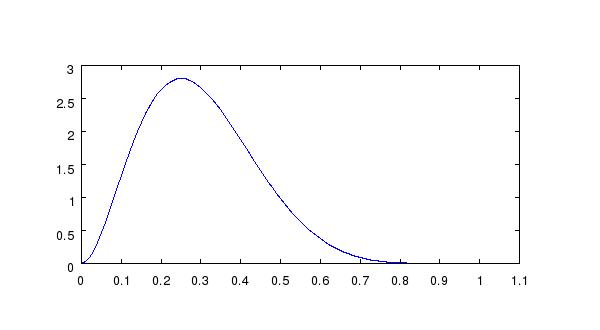
\includegraphics[width=8cm]{betapdf}}

If we generate a few random deviates with these values,
we see they are distributed around the peak of roughly
\verb|0.25|.
\begin{verbatim}
--> randbeta(3*ones(1,5),7*ones(1,5))

ans = 
    0.2777    0.0642    0.3305    0.5259    0.4003 
\end{verbatim}

\section{RANDBIN Generate Binomial Random Variables}

\subsection{Usage}

Generates random variables with a binomial distribution.
The general syntax for its use is
\begin{verbatim}
   y = randbin(N,p)
\end{verbatim}
where \verb|N| is a vector representing the number of Bernoulli
trials, and \verb|p| is the success probability associated with each
trial.
\subsection{Function Internals}

A Binomial random variable describes the number of successful
outcomes from \verb|N| Bernoulli trials, with the probability of
success in each trial being \verb|p|.  The probability distribution
is
\[
   P(n) = \frac{N!}{n!(N-n)!}p^n(1-p)^{N-n}
\]
\subsection{Example}

Here we generate \verb|10| binomial random variables, corresponding
to \verb|N=100| trials, each with probability \verb|p=0.1|, using
both \verb|randbin| and then again using \verb|rand| (to simulate the trials):
@>

\section{RANDCHI Generate Chi-Square Random Variable}

\subsection{Usage}

Generates a vector of chi-square random variables with the
given number of degrees of freedom.  The general syntax for
its use is 
\begin{verbatim}
   y = randchi(n)
\end{verbatim}
where \verb|n| is an array containing the degrees of freedom for
each generated random variable.
\subsection{Function Internals}

A chi-square random variable is essentially distributed as
the squared Euclidean norm of a vector of standard Gaussian random 
variables.  The number of degrees of freedom is generally the
number of elements in the vector.  In general, the PDF of
a chi-square random variable is
\[
 f(x) = \frac{x^{r/2-1}e^{-x/2}}{\Gamma(r/2)2^{r/2}}
\]
\subsection{Example}

First, a plot of the PDF for a family of chi-square random variables
\begin{verbatim}
--> f = zeros(7,100);
--> x = (1:100)/10;
--> for n=1:7;t=x.^(n/2-1).*exp(-x/2);f(n,:)=10*t/sum(t);end
--> plot(x,f');
\end{verbatim}
The PDF is below:


\centerline{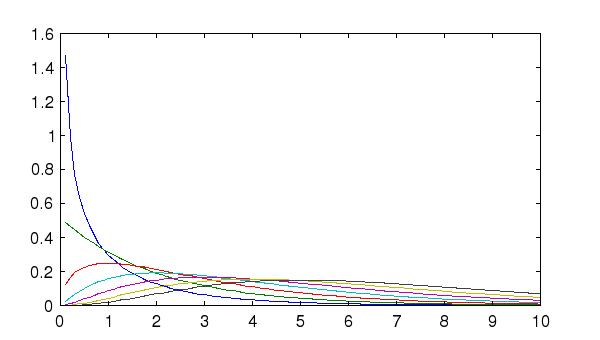
\includegraphics[width=8cm]{chipdf}}

Here is an example of using \verb|randchi| and \verb|randn| to compute
some chi-square random variables with four degrees of freedom.
\begin{verbatim}
--> randchi(4*ones(1,6))

ans = 
    8.9675    4.0015    3.2578    5.5461    2.5090    5.7587 

--> sum(randn(4,6).^2)

ans = 
    1.1941   10.6441    3.6228    8.4425    2.5031    1.9058 
\end{verbatim}

\section{RANDEXP Generate Exponential Random Variable}

\subsection{Usage}

Generates a vector of exponential random variables with
the specified parameter.  The general syntax for its use is
\begin{verbatim}
   y = randexp(lambda)
\end{verbatim}
where \verb|lambda| is a vector containing the parameters for
the generated random variables.
\subsection{Function Internals}

The exponential random variable is usually associated with
the waiting time between events in a Poisson random process.
The PDF of an exponential random variable is:
\[
   f(x) = \lambda e^{-\lambda x}
\]
\subsection{Example}

Here is an example of using the \verb|randexp| function to generate
some exponentially distributed random variables
@>

\section{RANDF Generate F-Distributed Random Variable}

\subsection{Usage}

Generates random variables with an F-distribution.  The general
syntax for its use is
\begin{verbatim}
   y = randf(n,m)
\end{verbatim}
where \verb|n| and \verb|m| are vectors of the number of degrees of freedom
in the numerator and denominator of the chi-square random variables
whose ratio defines the statistic.
\subsection{Function Internals}

The statistic \verb|F_{n,m}| is defined as the ratio of two chi-square
random variables:
\[
  F_{n,m} = \frac{\chi_n^2/n}{\chi_m^2/m}
\]
The PDF is given by
\[
  f_{n,m} = \frac{m^{m/2}n^{n/2}x^{n/2-1}}{(m+nx)^{(n+m)/2}B(n/2,m/2)},
\]
where \verb|B(a,b)| is the beta function.
\subsection{Example}

Here we use \verb|randf| to generate some F-distributed random variables,
and then again using the \verb|randchi| function:
\begin{verbatim}
--> randf(5*ones(1,9),7)

ans = 

 Columns 1 to 8

    1.1944    0.9069    0.7558    1.5029    0.0621    1.3860    1.8161    0.3755 

 Columns 9 to 9

    3.5794 

--> randchi(5*ones(1,9))./randchi(7*ones(1,9))

ans = 

 Columns 1 to 8

    1.3085    1.2693    1.0684    0.4377    1.1158    0.7171    0.4151    1.8022 

 Columns 9 to 9

    1.4606 
\end{verbatim}

\section{RANDGAMMA Generate Gamma-Distributed Random Variable}

\subsection{Usage}

Generates random variables with a gamma distribution.  The general
syntax for its use is
\begin{verbatim}
   y = randgamma(a,r),
\end{verbatim}
where \verb|a| and \verb|r| are vectors describing the parameters of the
gamma distribution.  Roughly speaking, if \verb|a| is the mean time between
changes of a Poisson random process, and we wait for the \verb|r| change,
the resulting wait time is Gamma distributed with parameters \verb|a| 
and \verb|r|.
\subsection{Function Internals}

The Gamma distribution arises in Poisson random processes.  It represents
the waiting time to the occurance of the \verb|r|-th event in a process with
mean time \verb|a| between events.  The probability distribution of a Gamma
random variable is
\[
   P(x) = \frac{a^r x^{r-1} e^{-ax}}{\Gamma(r)}.
\]
Note also that for integer values of \verb|r| that a Gamma random variable
is effectively the sum of \verb|r| exponential random variables with parameter
\verb|a|.
\subsection{Example}

Here we use the \verb|randgamma| function to generate Gamma-distributed
random variables, and then generate them again using the \verb|randexp|
function.
@>

\section{RANDI Uniformly Distributed Integer}

\subsection{Usage}

Generates an array of uniformly distributed integers between
the two supplied limits.  The general syntax for \verb|randi| is
\begin{verbatim}
   y = randi(low,high)
\end{verbatim}
where \verb|low| and \verb|high| are arrays of integers.  Scalars
can be used for one of the arguments.  The output \verb|y| is
a uniformly distributed pseudo-random number between \verb|low|
and \verb|high| (inclusive).
\subsection{Example}

Here is an example of a set of random integers between 
zero and 5:
@>

\section{RANDMULTI Generate Multinomial-distributed Random Variables}

\subsection{Usage}

This function generates samples from a multinomial distribution
given the probability of each outcome.  The general syntax for
its use is
\begin{verbatim}
   y = randmulti(N,pvec)
\end{verbatim}
where \verb|N| is the number of experiments to perform, and \verb|pvec|
is the vector of probabilities describing the distribution of
outcomes.
\subsection{Function Internals}

A multinomial distribution describes the number of times each
of \verb|m| possible outcomes occurs out of \verb|N| trials, where each
outcome has a probability \verb|p_i|.  More generally, suppose that
the probability of a Bernoulli random variable \verb|X_i| is \verb|p_i|,
and that 
\[
   \sum_{i=1}^{m} p_i = 1.
\]
Then the probability that \verb|X_i| occurs \verb|x_i| times is
\[
   P_N(x_1,x_2,\ldots,x_n) = \frac{N!}{x_1!\cdots x_n!} p_1^{x_1}\cdots p_n^{x_n}.
\]
\subsection{Example}

Suppose an experiment has three possible outcomes, say heads,
tails and edge, with probabilities \verb|0.4999|, \verb|0.4999| and
\verb|0.0002|, respectively.  Then if we perform ten thousand coin
flips we get
\begin{verbatim}
--> randmulti(10000,[0.4999,0.4999,0.0002])

ans = 
 5026 4973    1 
\end{verbatim}

\section{RANDN Gaussian (Normal) Random Number Generator}

\subsection{Usage}

Creates an array of pseudo-random numbers of the specified size.
The numbers are normally distributed with zero mean and a unit
standard deviation (i.e., \verb|mu = 0, sigma = 1|). 
 Two seperate syntaxes are possible.  The first syntax specifies the array 
dimensions as a sequence of scalar dimensions:
\begin{verbatim}
  y = randn(d1,d2,...,dn).
\end{verbatim}
The resulting array has the given dimensions, and is filled with
random numbers.  The type of \verb|y| is \verb|double|, a 64-bit floating
point array.  To get arrays of other types, use the typecast 
functions.
    
The second syntax specifies the array dimensions as a vector,
where each element in the vector specifies a dimension length:
\begin{verbatim}
  y = randn([d1,d2,...,dn]).
\end{verbatim}
This syntax is more convenient for calling \verb|randn| using a 
variable for the argument.

Finally, \verb|randn| supports two additional forms that allow
you to manipulate the state of the random number generator.
The first retrieves the state
\begin{verbatim}
  y = randn('state')
\end{verbatim}
which is a 625 length integer vector.  The second form sets
the state
\begin{verbatim}
  randn('state',y)
\end{verbatim}
or alternately, you can reset the random number generator with
\begin{verbatim}
  randn('state',0)
\end{verbatim}
\subsection{Function Internals}

Recall that the
probability density function (PDF) of a normal random variable is
\[
f(x) = \frac{1}{\sqrt{2\pi \sigma^2}} e^{\frac{-(x-\mu)^2}{2\sigma^2}}.
\]
The Gaussian random numbers are generated from pairs of uniform random numbers using a transformation technique. 
\subsection{Example}

The following example demonstrates an example of using the first form of the \verb|randn| function.
\begin{verbatim}
--> randn(2,2,2)

ans = 

(:,:,1) = 

   -1.7375   -0.5664 
   -0.2634   -1.0112 

(:,:,2) = 

   -0.4020    0.0557 
   -1.8966    0.2098 
\end{verbatim}
The second example demonstrates the second form of the \verb|randn| function.
\begin{verbatim}
--> randn([2,2,2])

ans = 

(:,:,1) = 

   -0.7183    1.9415 
    0.1010   -1.1747 

(:,:,2) = 

    0.3048    3.1685 
   -1.4185   -0.6130 
\end{verbatim}
In the next example, we create a large array of 10000  normally distributed pseudo-random numbers.  We then shift the mean to 10, and the variance to 5.  We then numerically calculate the mean and variance using \verb|mean| and \verb|var|, respectively.
\begin{verbatim}
--> x = 10+sqrt(5)*randn(1,10000);
--> mean(x)

ans = 

   10.0135 

--> var(x)

ans = 

    4.9458 
\end{verbatim}
Now, we use the state manipulation functions of \verb|randn| to exactly reproduce 
a random sequence.  Note that unlike using \verb|seed|, we can exactly control where
the random number generator starts by saving the state.
\begin{verbatim}
--> randn('state',0)    % restores us to startup conditions
--> a = randn(1,3)      % random sequence 1

a = 

   -0.0362   -0.1404    0.6934 

--> b = randn('state'); % capture the state vector
--> c = randn(1,3)      % random sequence 2  

c = 

    0.5998    0.7086   -0.9394 

--> randn('state',b);   % restart the random generator so...
--> c = randn(1,3)      % we get random sequence 2 again

c = 

    0.5998    0.7086   -0.9394 
\end{verbatim}

\section{RANDNBIN Generate Negative Binomial Random Variables}

\subsection{Usage}

Generates random variables with a negative binomial distribution.
The general syntax for its use is
\begin{verbatim}
   y = randnbin(r,p)
\end{verbatim}
where \verb|r| is a vector of integers representing the number of
successes, and \verb|p| is the probability of success.
\subsection{Function Internals}

A negative binomial random variable describes the number of failures
\verb|x| that occur in \verb|x+r| bernoulli trials, with a success on the 
\verb|x+r| trial.  The pdf is given by
\[
  P_{r,p}(x)=\left(\begin{matrix} x+r-1 \\ r-1 \end{matrix}\right)p^r(1-p)^x.
\]
\subsection{Example}

Here we generate some negative binomial random variables:
\begin{verbatim}
--> randnbin(3*ones(1,4),.01)

ans = 
 437 215 199 187 

--> randnbin(6*ones(1,4),.01)

ans = 
  471 1233  768  338 
\end{verbatim}

\section{RANDNCHI Generate Noncentral Chi-Square Random Variable}

\subsection{Usage}

Generates a vector of non-central chi-square random variables
with the given number of degrees of freedom and the given
non-centrality parameters.  The general syntax for its use is
\begin{verbatim}
   y = randnchi(n,mu)
\end{verbatim}
where \verb|n| is an array containing the degrees of freedom for
each generated random variable (with each element of \verb|n| >= 1),
and \verb|mu| is the non-centrality shift (must be positive).
\subsection{Function Internals}

A non-central chi-square random variable is the sum of a chisquare
deviate with \verb|n-1| degrees of freedom plus the square of a normal
deviate with mean \verb|mu| and standard deviation 1.
\subsection{Examples}

Here is an example of a non-central chi-square random variable:
\begin{verbatim}
--> randnchi(5*ones(1,9),0.3)

ans = 

 Columns 1 to 7

    1.7097    6.6003   14.1463    2.0817    4.4984    5.3132    3.1775 

 Columns 8 to 9

    3.5291    5.5185 
\end{verbatim}

\section{RANDNF Generate Noncentral F-Distribution Random Variable}

\subsection{Usage}

Generates a vector of non-central F-distributed random variables
with the specified parameters.  The general syntax for its use is
\begin{verbatim}
   y = randnf(n,m,c)
\end{verbatim}
where \verb|n| is the number of degrees of freedom in the numerator,
and \verb|m| is the number of degrees of freedom in the denominator.
The vector \verb|c| determines the non-centrality shift of the numerator.
\subsection{Function Internals}

A non-central F-distributed random variable is the ratio of a
non-central chi-square random variable and a central chi-square random
variable, i.e.,
\[
   F_{n,m,c} = \frac{\chi_{n,c}^2/n}{\chi_m^2/m}.
\]
\subsection{Example}

Here we use the \verb|randf| to generate some non-central F-distributed
random variables:
\begin{verbatim}
--> randnf(5*ones(1,9),7,1.34)

ans = 

 Columns 1 to 6

    1.9422    0.5987    0.1890    0.7468    2.3759    8.2553 

 Columns 7 to 9

    1.8047    0.2222    2.2680 
\end{verbatim}

\section{RANDP Generate Poisson Random Variable}

\subsection{Usage}

Generates a vector Poisson random variables with the given
parameters.  The general syntax for its use is
\begin{verbatim}
   y = randp(nu),
\end{verbatim}
where \verb|nu| is an array containing the rate parameters
for the generated random variables.  
\subsection{Function Internals}

A Poisson random variable is generally defined by taking the
limit of a binomial distribution as the sample size becomes
large, with the expected number of successes being fixed (so
that the probability of success decreases as \verb|1/N|).  
The Poisson distribution is given by
\[
  P_{\nu}(n) = \frac{\nu^n e^{-nu}}{n!}.
\]
\subsection{Example}

Here is an exmaple of using \verb|randp| to generate some Poisson
random variables, and also using \verb|randbin| to do the same
using \verb|N=1000| trials to approximate the Poisson result.
\begin{verbatim}
--> randp(33*ones(1,10))

ans = 
 31 33 34 44 32 29 34 30 32 32 

--> randbin(1000*ones(1,10),33/1000*ones(1,10))

ans = 
 32 36 36 39 33 34 41 33 42 32 
\end{verbatim}

\section{RANDPERM Random permutation}

\subsection{USAGE}

\begin{verbatim}
   y = randperm(n)
\end{verbatim}
\verb|y| is a random permutation of integers from 1 to \verb|n|.
\verb|randperm| calls \verb|rand| and changes its state.
\subsection{Example}

@>

\section{SEED Seed the Random Number Generator}

\subsection{Usage}

Seeds the random number generator using the given integer seeds.  
Changing the seed allows you to choose which pseudo-random
sequence is generated.  The seed takes two \verb|uint32| values:
\begin{verbatim}
  seed(s,t)
\end{verbatim}
where \verb|s| and \verb|t| are the seed values.  Note that due to limitations
in \verb|ranlib|, the values of \verb|s,t| must be between \verb|0 <= s,t <= 2^30|.
\subsection{Example}

Here's an example of how the seed value can be used to reproduce
a specific random number sequence.
\begin{verbatim}
--> seed(32,41);
--> rand(1,5)

ans = 

    0.8589    0.3727    0.5551    0.9557    0.7367 

--> seed(32,41);
--> rand(1,5)

ans = 

    0.8589    0.3727    0.5551    0.9557    0.7367 
\end{verbatim}

\chapter{Input/Ouput Functions}
\section{CSVREAD Read Comma Separated Value (CSV) File}

\subsection{Usage}

The \verb|csvread| function reads a text file containing comma
separated values (CSV), and returns the resulting numeric
matrix (2D).  The function supports multiple syntaxes.  The
first syntax for \verb|csvread| is 
\begin{verbatim}
   x = csvread('filename')
\end{verbatim}
which attempts to read the entire CSV file into array \verb|x|.
The file can contain only numeric values.  Each entry in the
file should be separated from other entries by a comma.  However,
FreeMat will attempt to make sense of the entries if the comma
is missing (e.g., a space separated file will also parse correctly).
For complex values, you must be careful with the spaces).  The second
form of \verb|csvread| allows you to specify the first row and column 
(zero-based index)
\begin{verbatim}
  x = csvread('filename',firstrow,firstcol)
\end{verbatim}
The last form allows you to specify the range to read also.  This form
is
\begin{verbatim}
  x = csvread('filename',firstrow,firstcol,readrange)
\end{verbatim}
where \verb|readrange| is either a 4-vector of the form \verb|[R1,C1,R2,C2]|,
where \verb|R1,C1| is the first row and column to use, and \verb|R2,C2| is the
last row and column to use.  You can also specify the \verb|readrange| as
a spreadsheet range \verb|B12..C34|, in which case the index for the
range is 1-based (as in a typical spreadsheet), so that \verb|A1| is the
first cell in the upper left corner. Note also that \verb|csvread| is
somewhat limited. 
\subsection{Example}

Here is an example of a CSV file that we wish to read in
\begin{verbatim}
    sample_data.csv
10, 12, 13, 00, 45, 16
09, 11, 52, 93, 05, 06
01, 03, 04, 04, 90, -3
14, 17, 13, 67, 30, 43
21, 33, 14, 44, 01, 00
\end{verbatim}
We start by reading the entire file
\begin{verbatim}
--> csvread('sample_data.csv')

ans = 
 10 12 13  0 45 16 
  9 11 52 93  5  6 
  1  3  4  4 90 -3 
 14 17 13 67 30 43 
 21 33 14 44  1  0 
\end{verbatim}
Next, we read everything starting with the second row, and third column
\begin{verbatim}
--> csvread('sample_data.csv',1,2)

ans = 
 52 93  5  6 
  4  4 90 -3 
 13 67 30 43 
 14 44  1  0 
\end{verbatim}
Finally, we specify that we only want the \verb|3 x 3| submatrix starting
with the second row, and third column
\begin{verbatim}
--> csvread('sample_data.csv',1,2,[1,2,3,4])

ans = 
 52 93  5 
  4  4 90 
 13 67 30 
\end{verbatim}
\begin{verbatim}
    sample_data.csv
10, 12, 13, 00, 45, 16
09, 11, 52, 93, 05, 06
01, 03, 04, 04, 90, -3
14, 17, 13, 67, 30, 43
21, 33, 14, 44, 01, 00
\end{verbatim}

\section{CSVWRITE Write Comma Separated Value (CSV) File}

\subsection{Usage}

The \verb|csvwrite| function writes a given matrix to a text
file using comma separated value (CSV) notation.  Note that
you can create CSV files with arbitrary sized matrices, but
that \verb|csvread| has limits on line length.  If you need to
reliably read and write large matrices, use \verb|rawwrite| and
\verb|rawread| respectively.  The syntax for \verb|csvwrite| is 
\begin{verbatim}
   csvwrite('filename',x)
\end{verbatim}
where \verb|x| is a numeric array.  The contents of \verb|x| are written
to \verb|filename| as comma-separated values.  You can also specify
a row and column offset to \verb|csvwrite| to force \verb|csvwrite| to
write the matrix \verb|x| starting at the specified location in the 
file.  This syntax of the function is
\begin{verbatim}
   csvwrite('filename',x,startrow,startcol)
\end{verbatim}
where \verb|startrow| and \verb|startcol| are the offsets in zero-based
indexing.  
\subsection{Example}

Here we create a simple matrix, and write it to a CSV file
\begin{verbatim}
--> x = [1,2,3;5,6,7]

x = 
 1 2 3 
 5 6 7 

--> csvwrite('csvwrite.csv',x)
--> csvread('csvwrite.csv')

ans = 
 1 2 3 
 5 6 7 
\end{verbatim}
Next, we do the same with an offset.
\begin{verbatim}
--> csvwrite('csvwrite.csv',x,1,2)
--> csvread('csvwrite.csv')

ans = 
 0 0 0 0 
 0 1 2 3 
 0 5 6 7 
\end{verbatim}
Note the extra zeros.

\section{DISP Display a Variable or Expression}

\subsection{Usage}

Displays the result of a set of expressions.  The \verb|disp| function
takes a variable number of arguments, each of which is an expression
to output:
\begin{verbatim}
  disp(expr1,expr2,...,exprn)
\end{verbatim}
This is functionally equivalent to evaluating each of the expressions
without a semicolon after each.
\subsection{Example}

Here are some simple examples of using \verb|disp|.
\begin{verbatim}
--> a = 32;
--> b = 1:4;
--> disp(a,b,pi)

 32 


 1 2 3 4 


    3.1416 
\end{verbatim}

\section{DLMREAD Read ASCII-delimited File}

\subsection{Usage}

Loads a matrix from an ASCII-formatted text file with a delimiter
between the entries.  This function is similar to the \verb|load -ascii|
command, except that it can handle complex data, and it allows you
to specify the delimiter.  Also, you can read only a subset of the
data from the file.  The general syntax for the \verb|dlmread| function
is
\begin{verbatim}
    y = dlmread(filename)
\end{verbatim}
where \verb|filename| is a string containing the name of the file to read.
In this form, FreeMat will guess at the type of the delimiter in the 
file.  The guess is made by examining the input for common delimiter
characters, which are \verb|,;:| or a whitespace (e.g., tab).  The text
in the file is preprocessed to replace these characters with whitespace
and the file is then read in using a whitespace for the delimiter.

If you know the delimiter in the file, you can specify it using
this form of the function:
\begin{verbatim}
    y = dlmread(filename, delimiter)
\end{verbatim}
where \verb|delimiter| is a string containing the delimiter.  If \verb|delimiter|
is the empty string, then the delimiter is guessed from the file.

You can also read only a portion of the file by specifying a start row
and start column:
\begin{verbatim}
    y = dlmread(filename, delimiter, startrow, startcol)
\end{verbatim}
where \verb|startrow| and \verb|startcol| are zero-based.  You can also specify
the data to read using a range argument:
\begin{verbatim}
    y = dlmread(filename, delimiter, range)
\end{verbatim}
where \verb|range| is either a vector \verb|[startrow,startcol,stoprow,stopcol]|
or is specified in spreadsheet notation as \verb|B4..ZA5|.

Note that complex numbers can be present in the file if they are encoded
without whitespaces inside the number, and use either \verb|i| or \verb|j| as 
the indicator.  Note also that when the delimiter is given, each incidence
of the delimiter counts as a separator.  Multiple separators generate
zeros in the matrix.

\section{FCLOSE File Close Function}

\subsection{Usage}

Closes a file handle, or all open file handles.  The general syntax
for its use is either
\begin{verbatim}
  fclose(handle)
\end{verbatim}
or
\begin{verbatim}
  fclose('all')
\end{verbatim}
In the first case a specific file is closed,  In the second, all open
files are closed.  Note that until a file is closed the file buffers
are not flushed.  Returns a '0' if the close was successful and a '-1' if
the close failed for some reason.
\subsection{Example}

A simple example of a file being opened with \verb|fopen| and then closed with \verb|fclose|.
\begin{verbatim}
--> fp = fopen('test.dat','wb','ieee-le')

fp = 
 12 

--> fclose(fp)
\end{verbatim}

\section{FEOF End Of File Function}

\subsection{Usage}

Check to see if we are at the end of the file.  The usage is
\begin{verbatim}
  b = feof(handle)
\end{verbatim}
The \verb|handle| argument must be a valid and active file handle.  The
return is true (logical 1) if the current position is at the end of
the file, and false (logical 0) otherwise.  Note that simply reading
to the end of a file will not cause \verb|feof| to return \verb|true|.  
You must read past the end of the file (which will cause an error 
anyway).  See the example for more details.
\subsection{Example}

Here, we read to the end of the file to demonstrate how \verb|feof| works.
At first pass, we force a read of the contents of the file by specifying
\verb|inf| for the dimension of the array to read.  We then test the
end of file, and somewhat counter-intuitively, the answer is \verb|false|.
We then attempt to read past the end of the file, which causes an
error.  An \verb|feof| test now returns the expected value of \verb|true|.
@>

\section{FFLUSH Force File Flush}

\subsection{Usage}

Flushes any pending output to a given file.  The general use of
this function is
\begin{verbatim}
   fflush(handle)
\end{verbatim}
where \verb|handle| is an active file handle (as returned by \verb|fopen|).

\section{FGETLINE Read a String from a File}

\subsection{Usage}

Reads a string from a file.  The general syntax for its use
is
\begin{verbatim}
  s = fgetline(handle)
\end{verbatim}
This function reads characters from the file \verb|handle| into
a \verb|string| array \verb|s| until it encounters the end of the file
or a newline.  The newline, if any, is retained in the output
string.  If the file is at its end, (i.e., that \verb|feof| would
return true on this handle), \verb|fgetline| returns an empty
string.
\subsection{Example}

First we write a couple of strings to a test file.
\begin{verbatim}
--> fp = fopen('testtext','w');
--> fprintf(fp,'String 1\n');
--> fprintf(fp,'String 2\n');
--> fclose(fp);
\end{verbatim}
Next, we read then back.
\begin{verbatim}
--> fp = fopen('testtext','r')

fp = 
 4 

--> fgetline(fp)

ans = 
String 1

--> fgetline(fp)

ans = 
String 2

--> fclose(fp);
\end{verbatim}

\section{FOPEN File Open Function}

\subsection{Usage}

Opens a file and returns a handle which can be used for subsequent
file manipulations.  The general syntax for its use is
\begin{verbatim}
  fp = fopen(fname,mode,byteorder)
\end{verbatim}
Here \verb|fname| is a string containing the name of the file to be 
opened.  \verb|mode| is the mode string for the file open command.
The first character of the mode string is one of the following:
\begin{itemize}
\item  \verb|'r'|  Open  file  for  reading.  The file pointer is placed at
          the beginning of the file.  The file can be read from, but
	  not written to.

\item  \verb|'r+'|   Open for reading and writing.  The file pointer is
          placed at the beginning of the file.  The file can be read
	  from and written to, but must exist at the outset.

\item  \verb|'w'|    Open file for writing.  If the file already exists, it is
          truncated to zero length.  Otherwise, a new file is
	  created.  The file pointer is placed at the beginning of
	  the file.

\item  \verb|'w+'|   Open for reading and writing.  The file is created  if  
          it  does not  exist, otherwise it is truncated to zero
	  length.  The file pointer placed at the beginning of the file.

\item  \verb|'a'|    Open for appending (writing at end of file).  The file  is  
          created  if it does not exist.  The file pointer is placed at
	  the end of the file.

\item  \verb|'a+'|   Open for reading and appending (writing at end of file).   The
          file  is created if it does not exist.  The file pointer is
	  placed at the end of the file.

\end{itemize}
Starting with FreeMat 4, all files are treated as binary files by default.
To invoke the operating systems 'CR/LF <-> CR' translation (on Win32)
add a 't' to the mode string, as in 'rt+'.

Also, you can supply a second argument to \verb|fopen| to retrieve error
messages if the \verb|fopen| fails.
\begin{verbatim}
  [fp,messages] = fopen(fname,mode,byteorder)
\end{verbatim}

Finally, FreeMat has the ability to read and write files of any
byte-sex (endian).  The third (optional) input indicates the 
byte-endianness of the file.  If it is omitted, the native endian-ness
of the machine running FreeMat is used.  Otherwise, the third
argument should be one of the following strings:
\begin{itemize}
\item  \verb|'le','ieee-le','little-endian','littleEndian','little','l','ieee-le.l64','s'|

\item  \verb|'be','ieee-be','big-endian','bigEndian','big','b','ieee-be.l64','a'|

\end{itemize}
	
If the file cannot be opened, or the file mode is illegal, then
an error occurs. Otherwise, a file handle is returned (which is
an integer).  This file handle can then be used with \verb|fread|,
\verb|fwrite|, or \verb|fclose| for file access.

Note that three handles are assigned at initialization time:
\begin{itemize}
\item  Handle 0 - is assigned to standard input

\item  Handle 1 - is assigned to standard output

\item  Handle 2 - is assigned to standard error

\end{itemize}
These handles cannot be closed, so that user created file handles start at \verb|3|.

\subsection{Examples}

Here are some examples of how to use \verb|fopen|.  First, we create a new 
file, which we want to be little-endian, regardless of the type of the machine.
We also use the \verb|fwrite| function to write some floating point data to
the file.
\begin{verbatim}
--> fp = fopen('test.dat','w','ieee-le')

fp = 

 8 

--> fwrite(fp,float([1.2,4.3,2.1]))

ans = 

 12 

--> fclose(fp)
\end{verbatim}
Next, we open the file and read the data back
\begin{verbatim}
--> fp = fopen('test.dat','r','ieee-le')

fp = 

 8 

--> fread(fp,[1,3],'float')

ans = 

    1.2000    4.3000    2.1000 

--> fclose(fp)
\end{verbatim}
Now, we re-open the file in append mode and add two additional \verb|float|s to the
file.
\begin{verbatim}
--> fp = fopen('test.dat','a+','le')

fp = 

 8 

--> fwrite(fp,float([pi,e]))

ans = 

 8 

--> fclose(fp)
\end{verbatim}
Finally, we read all 5 \verb|float| values from the file
\begin{verbatim}
--> fp = fopen('test.dat','r','ieee-le')

fp = 

 8 

--> fread(fp,[1,5],'float')

ans = 

    1.2000    4.3000    2.1000    3.1416    2.7183 

--> fclose(fp)
\end{verbatim}

\section{FORMAT Control the Format of Matrix Display}

\subsection{Usage}

FreeMat supports several modes for displaying matrices (either through the
\verb|disp| function or simply by entering expressions on the command line.  
There are several options for the format command.  The default mode is equivalent
to
\begin{verbatim}
   format short
\end{verbatim}
which generally displays matrices with 4 decimals, and scales matrices if the entries
have magnitudes larger than roughly \verb|1e2| or smaller than \verb|1e-2|.   For more 
information you can use 
\begin{verbatim}
   format long
\end{verbatim}
which displays roughly 7 decimals for \verb|float| and \verb|complex| arrays, and 14 decimals
for \verb|double| and \verb|dcomplex|.  You can also use
\begin{verbatim}
   format short e
\end{verbatim}
to get exponential format with 4 decimals.  Matrices are not scaled for exponential 
formats.  Similarly, you can use
\begin{verbatim}
   format long e
\end{verbatim}
which displays the same decimals as \verb|format long|, but in exponential format.
You can also use the \verb|format| command to retrieve the current format:
\begin{verbatim}
   s = format
\end{verbatim}
where \verb|s| is a string describing the current format.
\subsection{Example}

We start with the short format, and two matrices, one of double precision, and the
other of single precision.
\begin{verbatim}
--> format short
--> a = randn(4)

a = 
   -0.3756    0.0920    0.9516    1.8527 
    0.5078   -0.2088   -0.3120   -0.2380 
    0.5578    0.7695    0.0226    2.9326 
   -0.4420   -0.4871   -0.7582   -0.5059 

--> b = float(randn(4))

b = 
    0.2010    0.3416    0.1562   -0.5460 
    1.2842   -0.3808   -1.2720   -0.3398 
   -0.7660   -0.6251    2.4811    0.7956 
   -0.1727    0.8577    1.5701   -1.5048 
\end{verbatim}
Note that in the short format, these two matrices are displayed with the same format.
In \verb|long| format, however, they display differently
\begin{verbatim}
--> format long
--> a

ans = 
  -0.37559630424227   0.09196341864118   0.95155934364300   1.85265231634028 
   0.50776589164635  -0.20877480315311  -0.31198760445638  -0.23799081322695 
   0.55783547335483   0.76954243414671   0.02264031516947   2.93263318869123 
  -0.44202929771190  -0.48708606879623  -0.75822963661106  -0.50590405332950 

--> b

ans = 
   0.2010476   0.3415550   0.1561587  -0.5460028 
   1.2841575  -0.3808453  -1.2719837  -0.3397521 
  -0.7659672  -0.6251388   2.4811494   0.7956446 
  -0.1726678   0.8576548   1.5701485  -1.5048176 
\end{verbatim}
Note also that we we scale the contents of the matrices, FreeMat rescales the entries
with a scale premultiplier.
\begin{verbatim}
--> format short
--> a*1e4

ans = 

   1.0e+04 * 
   -0.3756    0.0920    0.9516    1.8527 
    0.5078   -0.2088   -0.3120   -0.2380 
    0.5578    0.7695    0.0226    2.9326 
   -0.4420   -0.4871   -0.7582   -0.5059 

--> a*1e-4

ans = 

   1.0e-04 * 
   -0.3756    0.0920    0.9516    1.8527 
    0.5078   -0.2088   -0.3120   -0.2380 
    0.5578    0.7695    0.0226    2.9326 
   -0.4420   -0.4871   -0.7582   -0.5059 

--> b*1e4

ans = 

   1.0e+04 * 
    0.2010    0.3416    0.1562   -0.5460 
    1.2842   -0.3808   -1.2720   -0.3398 
   -0.7660   -0.6251    2.4811    0.7956 
   -0.1727    0.8577    1.5701   -1.5048 

--> b*1e-4

ans = 

   1.0e-04 * 
    0.2010    0.3416    0.1562   -0.5460 
    1.2842   -0.3808   -1.2720   -0.3398 
   -0.7660   -0.6251    2.4811    0.7956 
   -0.1727    0.8577    1.5701   -1.5048 
\end{verbatim}
Next, we use the exponential formats:
\begin{verbatim}
--> format short e
--> a*1e4

ans = 
 -3.7560e+03  9.1963e+02  9.5156e+03  1.8527e+04 
  5.0777e+03 -2.0877e+03 -3.1199e+03 -2.3799e+03 
  5.5784e+03  7.6954e+03  2.2640e+02  2.9326e+04 
 -4.4203e+03 -4.8709e+03 -7.5823e+03 -5.0590e+03 

--> a*1e-4

ans = 
 -3.7560e-05  9.1963e-06  9.5156e-05  1.8527e-04 
  5.0777e-05 -2.0877e-05 -3.1199e-05 -2.3799e-05 
  5.5784e-05  7.6954e-05  2.2640e-06  2.9326e-04 
 -4.4203e-05 -4.8709e-05 -7.5823e-05 -5.0590e-05 

--> b*1e4

ans = 
  2.0105e+03  3.4156e+03  1.5616e+03 -5.4600e+03 
  1.2842e+04 -3.8085e+03 -1.2720e+04 -3.3975e+03 
 -7.6597e+03 -6.2514e+03  2.4811e+04  7.9564e+03 
 -1.7267e+03  8.5765e+03  1.5701e+04 -1.5048e+04 

--> b*1e-4

ans = 
  2.0105e-05  3.4155e-05  1.5616e-05 -5.4600e-05 
  1.2842e-04 -3.8085e-05 -1.2720e-04 -3.3975e-05 
 -7.6597e-05 -6.2514e-05  2.4811e-04  7.9564e-05 
 -1.7267e-05  8.5765e-05  1.5701e-04 -1.5048e-04 
\end{verbatim}
Finally, if we assign the \verb|format| function to a variable, we can retrieve the 
current format:
\begin{verbatim}
--> format short
--> t = format

t = 
short
\end{verbatim}

\section{FPRINTF Formated File Output Function (C-Style)}

\subsection{Usage}

Prints values to a file.  The general syntax for its use is
\begin{verbatim}
  fprintf(fp,format,a1,a2,...).
\end{verbatim}
or, 
\begin{verbatim}
  fprintf(format,a1,a2,...).
\end{verbatim}
Here \verb|format| is the format string, which is a string that
controls the format of the output.  The values of the variables
\verb|ai| are substituted into the output as required.  It is
an error if there are not enough variables to satisfy the format
string.  Note that this \verb|fprintf| command is not vectorized!  Each
variable must be a scalar.  The value \verb|fp| is the file handle.  If \verb|fp| is omitted,
file handle \verb|1| is assumed, and the behavior of \verb|fprintf| is effectively equivalent to \verb|printf|. For
more details on the format string, see \verb|printf|.
\subsection{Examples}

A number of examples are present in the Examples section of the \verb|printf| command.

\section{FREAD File Read Function}

\subsection{Usage}

Reads a block of binary data from the given file handle into a variable
of a given shape and precision.  The general use of the function is
\begin{verbatim}
  A = fread(handle,size,precision)
\end{verbatim}
The \verb|handle| argument must be a valid value returned by the fopen 
function, and accessable for reading.  The \verb|size| argument determines
the number of values read from the file.  The \verb|size| argument is simply
a vector indicating the size of the array \verb|A|.  The \verb|size| argument
can also contain a single \verb|inf| dimension, indicating that FreeMat should
calculate the size of the array along that dimension so as to read as
much data as possible from the file (see the examples listed below for
more details).  The data is stored as columns in the file, not 
rows.
    
Alternately, you can specify two return values to the \verb|fread| function,
in which case the second value contains the number of elements read
\begin{verbatim}
   [A,count] = fread(...)
\end{verbatim}
where \verb|count| is the number of elements in \verb|A|.

The third argument determines the type of the data.  Legal values for this
argument are listed below:
\begin{itemize}
\item  'uint8','uchar','unsigned char' for an unsigned, 8-bit integer.

\item  'int8','char','integer*1' for a signed, 8-bit integer.

\item  'uint16','unsigned short' for an unsigned, 16-bit  integer.

\item  'int16','short','integer*2' for a signed, 16-bit integer.

\item  'uint32','unsigned int' for an unsigned, 32-bit integer.

\item  'int32','int','integer*4' for a signed, 32-bit integer.

\item  'single','float32','float','real*4' for a 32-bit floating point.

\item  'double','float64','real*8' for a 64-bit floating point.

\end{itemize}

Starting with FreeMat 4, the format for the third argument has changed.
If you specify only a type, such as \verb|'float'|, the data is read in as
single precision, but the output type is always \verb|'double'|.  This behavior
is consistent with Matlab.  If you want the output type to match the input
type (as was previous behavior in FreeMat), you must preface the precision
string with a \verb|'*'|.  Thus, the precision string \verb|'*float'| implies
that data is read in as single precision, and the output is also single
precision.

The third option is to specify the input and output types explicitly.
You can do this by specifiying a precision string of the form 
\verb|'type1 => type2'|, where \verb|'type1'| is the input type and 
\verb|'type2'| is the output type.  For example, if the input type is
\verb|'double'| and the output type is to be a \verb|'float'|, then a type spec
of \verb|'double => float'| should be used.

\subsection{Example}

First, we create an array of \verb|512 x 512| Gaussian-distributed \verb|float| random variables, and then writing them to a file called \verb|test.dat|.
\begin{verbatim}
--> A = float(randn(512));
--> fp = fopen('test.dat','w');
--> fwrite(fp,A);
--> fclose(fp);
\end{verbatim}
Read as many floats as possible into a row vector
\begin{verbatim}
--> fp = fopen('test.dat','r');
--> x = fread(fp,[1,inf],'float');
--> fclose(fp);
--> who x
  Variable Name       Type   Flags             Size
              x    double                    [1x262144]
\end{verbatim}
Note that \verb|x| is a \verb|double| array.  This behavior is new to FreeMat 4.
Read the same floats into a 2-D float array.
\begin{verbatim}
--> fp = fopen('test.dat','r');
--> x = fread(fp,[512,inf],'float');
--> fclose(fp);
--> who x
  Variable Name       Type   Flags             Size
              x    double                    [512x512]
\end{verbatim}
To read them as a single precision float array, we can use the
following form:
\begin{verbatim}
--> fp = fopen('test.dat','r');
--> x = fread(fp,[512,inf],'*float');
--> fclose(fp);
--> who x
  Variable Name       Type   Flags             Size
              x    single                    [512x512]
\end{verbatim}


\section{FSCANF Formatted File Input Function (C-Style)}

\subsection{Usage}

Reads values from a file.  The general syntax for its use is
\begin{verbatim}
  [a,count] = fscanf(handle,format,[size])
\end{verbatim}
Here \verb|format| is the format string, which is a string that
controls the format of the input, \verb|size| specifies the amount of data to be read. Values that are parsed
from the \verb|text| are stored in a. Note that fscanf is vectorized - the format string is reused as long as
there are entries in the \verb|text| string.
See \verb|printf| for a description of the format.  Note that if
the file is at the end-of-file, the fscanf will return 

\section{FSEEK Seek File To A Given Position}

\subsection{Usage}

Moves the file pointer associated with the given file handle to 
the specified offset (in bytes).  The usage is
\begin{verbatim}
  fseek(handle,offset,style)
\end{verbatim}
The \verb|handle| argument must be a value and active file handle.  The
\verb|offset| parameter indicates the desired seek offset (how much the
file pointer is moved in bytes).  The \verb|style| parameter determines
how the offset is treated.  Three values for the \verb|style| parameter
are understood:
\begin{itemize}
\item  string \verb|'bof'| or the value -1, which indicate the seek is relative
to the beginning of the file.  This is equivalent to \verb|SEEK_SET| in
ANSI C.

\item  string \verb|'cof'| or the value 0, which indicates the seek is relative
to the current position of the file.  This is equivalent to 
\verb|SEEK_CUR| in ANSI C.

\item  string \verb|'eof'| or the value 1, which indicates the seek is relative
to the end of the file.  This is equivalent to \verb|SEEK_END| in ANSI
C.

\end{itemize}
The offset can be positive or negative.
\subsection{Example}

The first example reads a file and then ``rewinds'' the file pointer by seeking to the beginning.
The next example seeks forward by 2048 bytes from the files current position, and then reads a line of 512 floats.
\begin{verbatim}
--> % First we create the file
--> fp = fopen('test.dat','wb');
--> fwrite(fp,float(rand(4096,1)));
--> fclose(fp);
--> % Now we open it
--> fp = fopen('test.dat','rb');
--> % Read the whole thing
--> x = fread(fp,[1,inf],'float');
--> % Rewind to the beginning
--> fseek(fp,0,'bof');
--> % Read part of the file
--> y = fread(fp,[1,1024],'float');
--> who x y
  Variable Name       Type   Flags             Size
              x    double                    [1 4096]
              y    double                    [1 1024]
--> % Seek 2048 bytes into the file
--> fseek(fp,2048,'cof');
--> % Read 512 floats from the file
--> x = fread(fp,[512,1],'float');
--> % Close the file
--> fclose(fp);
\end{verbatim}

\section{FTELL File Position Function}

\subsection{Usage}

Returns the current file position for a valid file handle.
The general use of this function is
\begin{verbatim}
  n = ftell(handle)
\end{verbatim}
The \verb|handle| argument must be a valid and active file handle.  The
return is the offset into the file relative to the start of the
file (in bytes).
\subsection{Example}

Here is an example of using \verb|ftell| to determine the current file 
position.  We read 512 4-byte floats, which results in the file 
pointer being at position 512*4 = 2048.
\begin{verbatim}
--> fp = fopen('test.dat','wb');
--> fwrite(fp,randn(512,1));
--> fclose(fp);
--> fp = fopen('test.dat','rb');
--> x = fread(fp,[512,1],'float');
--> ftell(fp)

ans = 

 2048 
\end{verbatim}

\section{FWRITE File Write Function}

\subsection{Usage}

Writes an array to a given file handle as a block of binary (raw) data.
The general use of the function is
\begin{verbatim}
  n = fwrite(handle,A)
\end{verbatim}
The \verb|handle| argument must be a valid value returned by the fopen 
function, and accessable for writing. The array \verb|A| is written to
the file a column at a time.  The form of the output data depends
on (and is inferred from) the precision of the array \verb|A|.  If the 
write fails (because we ran out of disk space, etc.) then an error
is returned.  The output \verb|n| indicates the number of elements
successfully written.

Note that unlike MATLAB, FreeMat 4 does not default to \verb|uint8| for
writing arrays to files.  Alternately, the type of the data to be
written to the file can be specified with the syntax
\begin{verbatim}
  n = fwrite(handle,A,type)
\end{verbatim}
where \verb|type| is one of the following legal values:
\begin{itemize}
\item  'uint8','uchar','unsigned char' for an unsigned, 8-bit integer.

\item  'int8','char','integer*1' for a signed, 8-bit integer.

\item  'uint16','unsigned short' for an unsigned, 16-bit  integer.

\item  'int16','short','integer*2' for a signed, 16-bit integer.

\item  'uint32','unsigned int' for an unsigned, 32-bit integer.

\item  'int32','int','integer*4' for a signed, 32-bit integer.

\item  'single','float32','float','real*4' for a 32-bit floating point.

\item  'double','float64','real*8' for a 64-bit floating point.

\end{itemize}

\subsection{Example}

Heres an example of writing an array of \verb|512 x 512| Gaussian-distributed \verb|float| random variables, and then writing them to a file called \verb|test.dat|.
@>

\section{GETLINE Get a Line of Input from User}

\subsection{Usage}

Reads a line (as a string) from the user.  This function has
two syntaxes.  The first is 
\begin{verbatim}
  a = getline(prompt)
\end{verbatim}
where \verb|prompt| is a prompt supplied to the user for the query.
The second syntax omits the \verb|prompt| argument:
\begin{verbatim}
  a = getline
\end{verbatim}
Note that this function requires command line input, i.e., it 
will only operate correctly for programs or scripts written
to run inside the FreeMat GUI environment or from the X11 terminal.
If you build a stand-alone application and expect it to operate 
cross-platform, do not use this function (unless you include
the FreeMat console in the final application).

\section{GETPRINTLIMIT Get Limit For Printing Of Arrays}

\subsection{Usage}

Returns the limit on how many elements of an array are printed
using either the \verb|disp| function or using expressions on the
command line without a semi-colon.  The default is set to 
one thousand elements.  You can increase or decrease this
limit by calling \verb|setprintlimit|.  This function is provided
primarily so that you can temporarily change the output truncation
and then restore it to the previous value (see the examples).
\begin{verbatim}
   n=getprintlimit
\end{verbatim}
where \verb|n| is the current limit in use.
\subsection{Example}

Here is an example of using \verb|getprintlimit| along with \verb|setprintlimit| to temporarily change the output behavior of FreeMat.
@>

\section{HTMLREAD Read an HTML Document into FreeMat}

\subsection{Usage}

Given a filename, reads an HTML document, (attempts to) parse it, and
returns the result as a FreeMat data structure.  The syntax for its
use is:
\begin{verbatim}
   p = htmlread(filename)
\end{verbatim}
where \verb|filename| is a \verb|string|.  The
resulting object \verb|p| is a data structure containing the information
in the document.  Note that this function works by internally converting
the HTML document into something closer to XHTML, and then using the
XML parser to parse it.  In some cases, the converted HTML cannot be properly
parsed.  In such cases, a third party tool such as ''tidy'' will probably do
a better job.

\section{IMREAD Read Image File To Matrix}

\subsection{Usage}

Reads the image data from the given file into a matrix.  Note that
FreeMat's support for \verb|imread| is not complete.  Only some of the
formats specified in the MATLAB API are implemented.  The syntax
for its use is
\begin{verbatim}
  [A,map,alpha] = imread(filename)
\end{verbatim}
where \verb|filename| is the name of the file to read from.  The returned
arrays \verb|A| contain the image data, \verb|map| contains the colormap information
(for indexed images), and \verb|alpha| contains the alphamap (transparency).
The returned values will depend on the type of the original image.  Generally
you can read images in the \verb|jpg,png,xpm,ppm| and some other formats.

\section{IMWRITE Write Matrix to Image File}

\subsection{Usage}

Write the image data from the matrix into a given file.  Note that
FreeMat's support for \verb|imwrite| is not complete.
You can write images in the \verb|jpg,png,xpm,ppm| and some other formats.
The syntax for its use is
\begin{verbatim}
  imwrite(A, filename)
  imwrite(A, map, filename)
  imwrite(A, map, filename, 'Alpha', alpha)

or Octave-style syntax:
  imwrite(filename, A)
  imwrite(filename, A, map)
  imwrite(filename, A, map, alpha)
\end{verbatim}
where \verb|filename| is the name of the file to write to.  The input array 
\verb|A| contains the image data (2D for gray or indexed, and 3D for color).  
If \verb|A| is an integer array (int8, uint8, int16, uint16, int32, uint32), 
the values of its elements should be within 0-255.  If \verb|A| is a 
floating-point array (float or double), the value of its elements should
be in the range [0,1].  \verb|map| contains the colormap information
(for indexed images), and \verb|alpha| the alphamap (transparency).
\subsection{Example}

Here is a simple example of \verb|imread|/\verb|imwrite|.  First, we generate
a grayscale image and save it to an image file.
@>
Then, we read image file and show it:
@>

\section{INPUT Get Input From User}

\subsection{Usage}

The \verb|input| function is used to obtain input from the user.  There are
two syntaxes for its use.  The first is
\begin{verbatim}
    r = input('prompt')
\end{verbatim}
in which case, the prompt is presented, and the user is allowed to enter
an expression.  The expression is evaluated in the current workspace or
context (so it can use any defined variables or functions), and returned
for assignment to the variable (\verb|r| in this case).  In the second form
of the \verb|input| function, the syntax is
\begin{verbatim}
    r = input('prompt','s')
\end{verbatim}
in which case the text entered by the user is copied verbatim to the
output.

\section{LOAD Load Variables From A File}

\subsection{Usage}

Loads a set of variables from a file in a machine independent format.
The \verb|load| function takes one argument:
\begin{verbatim}
  load filename,
\end{verbatim}
or alternately,
\begin{verbatim}
  load('filename')
\end{verbatim}
This command is the companion to \verb|save|.  It loads the contents of the
file generated by \verb|save| back into the current context.  Global and 
persistent variables are also loaded and flagged appropriately.  By
default, FreeMat assumes that files that end in a \verb|.mat| or \verb|.MAT|
extension are MATLAB-formatted files.  Also, FreeMat assumes that 
files that end in \verb|.txt| or \verb|.TXT| are ASCII files. 
For other filenames, FreeMat first tries to open the file as a 
FreeMat binary format file (as created by the \verb|save| function).  
If the file fails to open as a FreeMat binary file, then FreeMat 
attempts to read it as an ASCII file.  

You can force FreeMat to assume a particular format for the file
by using alternate forms of the \verb|load| command.  In particular,
\begin{verbatim}
  load -ascii filename
\end{verbatim}
will load the data in file \verb|filename| as an ASCII file (space delimited
numeric text) loaded into a single variable in the current workspace
with the name \verb|filename| (without the extension).

For MATLAB-formatted data files, you can use
\begin{verbatim}
  load -mat filename
\end{verbatim}
which forces FreeMat to assume that \verb|filename| is a MAT-file, regardless
of the extension on the filename.

You can also specify which variables to load from a file (not from 
an ASCII file - only single 2-D variables can be successfully saved and
retrieved from ASCII files) using the additional syntaxes of the \verb|load|
command.  In particular, you can specify a set of variables to load by name
\begin{verbatim}
  load filename Var_1 Var_2 Var_3 ...
\end{verbatim}
where \verb|Var_n| is the name of a variable to load from the file.  
Alternately, you can use the regular expression syntax
\begin{verbatim}
  load filename -regexp expr_1 expr_2 expr_3 ...
\end{verbatim}
where \verb|expr_n| is a regular expression (roughly as expected by \verb|regexp|).
Note that a simpler regular expression mechanism is used for this syntax
than the full mechanism used by the \verb|regexp| command.

Finally, you can use \verb|load| to create a variable containing the 
contents of the file, instead of automatically inserting the variables
into the curent workspace.  For this form of \verb|load| you must use the
function syntax, and capture the output:
\begin{verbatim}
  V = load('arg1','arg2',...)
\end{verbatim}
which returns a structure \verb|V| with one field for each variable
retrieved from the file.  For ASCII files, \verb|V| is a double precision
matrix.

\subsection{Example}

Here is a simple example of \verb|save|/\verb|load|.  First, we save some variables to a file.
\begin{verbatim}
--> D = {1,5,'hello'};
--> s = 'test string';
--> x = randn(512,1);
--> z = zeros(512);
--> who
  Variable Name       Type   Flags             Size
              D      cell                    [1 3]
              s      char                    [1 11]
              x    double                    [512 1]
              z    double                    [512 512]
--> save loadsave.dat
\end{verbatim}
Next, we clear the variables, and then load them back from the file.
\begin{verbatim}
--> clear D s x z
--> who
  Variable Name       Type   Flags             Size
            ans    double                    [0 0]
--> load loadsave.dat
--> who
  Variable Name       Type   Flags             Size
              D      cell                    [1 3]
            ans    double                    [0 0]
              s      char                    [1 11]
              x    double                    [512 1]
              z    double                    [512 512]
\end{verbatim}

\section{PAUSE Pause Script Execution}

\subsection{Usage}

The \verb|pause| function can be used to pause execution of FreeMat
scripts.  There are several syntaxes for its use.  The first form
is
\begin{verbatim}
   pause
\end{verbatim}
This form of the \verb|pause| function pauses FreeMat until you press
any key.  The second form of the \verb|pause| function takes an argument
\begin{verbatim}
   pause(p)
\end{verbatim}
where \verb|p| is the number of seconds to pause FreeMat for.  The pause
argument should be accurate to a millisecond on all supported platforms.
Alternately, you can control all \verb|pause| statements using:
\begin{verbatim}
   pause on
\end{verbatim}
which enables pauses and
\begin{verbatim}
   pause off
\end{verbatim}
which disables all \verb|pause| statements, both with and without arguments.

\section{PRINTF Formated Output Function (C-Style)}

\subsection{Usage}

Prints values to the output.  The general syntax for its use is
\begin{verbatim}
  printf(format,a1,a2,...)
\end{verbatim}
Here \verb|format| is the format string, which is a string that
controls the format of the output.  The values of the variables
\verb|a\_i| are substituted into the output as required.  It is
an error if there are not enough variables to satisfy the format
string.  Note that this \verb|printf| command is not vectorized!  Each
variable must be a scalar.

It is important to point out that the \verb|printf| function does not
add a newline (or carriage return) to the output by default.  That
can lead to some confusing behavior if you do not know what to expect.
For example, the command \verb|printf('Hello')| does not appear to
produce any output.  In fact, it does produce the text, but it then
gets overwritten by the prompt.  To see the text, you need 
\verb|printf('Hello\\n')|.  This seems odd, but allows you to assemble a
line using multiple \verb|printf| commands, including the \verb|'\\n'| when
you are done with the line.  You can also use the \verb|'\r'| character
as an explicit carriage return (with no line feed).  This allows you
to write to the same line many times (to show a progress string, for
example).

\subsection{Format of the format string}


The  format  string  is a character string, beginning and ending in its
initial shift state, if any.  The format string is composed of zero  or
more   directives:  ordinary  characters  (not  %),  which  are  copied
unchanged to the output stream; and conversion specifications, each  of
which results in fetching zero or more subsequent arguments.  Each 
conversion specification is introduced by the character %, and ends with a
conversion  specifier.  In between there may be (in this order) zero or
more flags, an optional minimum field width, and an optional precision.

The  arguments must correspond properly (after type promotion) with the
conversion specifier, and are used in the order given.

\subsection{The flag characters}

The character \verb|%| is followed by zero or more of the following flags:
\begin{itemize}
\item  \verb|\#|   The  value  should be converted to an ``alternate form''.  For \verb|o| conversions, the first character of the output  string  is  made  zero (by prefixing a \verb|0| if it was not zero already).  For \verb|x| and \verb|X| conversions, a nonzero result has the string \verb|'0x'| (or \verb|'0X'| for  \verb|X|  conversions) prepended to it.  For \verb|a, A, e, E, f, F, g,| and \verb|G|  conversions, the result will always  contain  a  decimal  point,  even  if  no digits follow it (normally, a decimal point appears  in the results of those conversions only if  a  digit  follows).  For \verb|g| and \verb|G| conversions, trailing zeros are not removed from the  result as they would otherwise be.  For other  conversions,  the  result is undefined.

\item  \verb|0|   The value should be zero padded.  For \verb|d, i, o, u, x, X, a, A, e, E, f, F, g,| and \verb|G| conversions, the converted value is padded  on the  left  with  zeros rather than blanks.  If the \verb|0| and \verb|-| flags  both appear, the \verb|0| flag is ignored.  If  a  precision  is  given  with  a numeric conversion \verb|(d, i, o, u, x, and X)|, the \verb|0| flag is  ignored.  For other conversions, the behavior is undefined.

\item  \verb|-|   The converted value is to be left adjusted on the  field  boundary.  (The default is right justification.) Except for \verb|n| conversions, the converted value is padded on the right  with  blanks, rather than on the left with blanks or zeros.  A \verb|-| overrides a \verb|0| if both are given.

\item  \verb|' '| (a space) A blank should be left before a  positive  number  (or empty string) produced by a signed conversion.

\item  \verb|+| A  sign  (\verb|+| or \verb|-|) always be placed before a number produced by a signed conversion.  By default a sign is used only for  negative numbers. A \verb|+| overrides a space if both are used.

\end{itemize}
\subsection{The field width}

An  optional decimal digit string (with nonzero first digit) specifying a 
minimum field width.  If the converted  value  has  fewer  characters than 
the  field  width,  it will be padded with spaces on the left (or right, 
if the left-adjustment flag has been given).  A  negative  field width is 
taken as a \verb|'-'| flag followed by a positive field  width. In no case does 
a non-existent or small field width cause truncation of a field; if the 
result of a conversion is wider than the  field  width, the field is 
expanded to contain the conversion result.

\subsection{The precision}


An  optional  precision,  in the form of a period (\verb|'.'|)  followed by an optional decimal digit string.  If the precision is given as just \verb|'.'|, or the precision is negative, the precision is  taken  to  be zero.   This  gives the minimum number of digits to appear for \verb|d, i, o, u, x|, and \verb|X| conversions, the number of digits to appear after the radix character  for  \verb|a, A, e, E, f|, and \verb|F| conversions, the maximum number of significant digits for \verb|g| and \verb|G| conversions, or the  maximum  number  of  characters to be printed from a string for s conversions.

\subsection{The conversion specifier}


A character that specifies the type of conversion to be  applied.   The
conversion specifiers and their meanings are:
\begin{itemize}
\item  \verb|d,i|   The  int  argument is converted to signed decimal notation.  The  precision, if any, gives the minimum number of digits that  must   appear;  if  the  converted  value  requires fewer digits, it is    padded on the left with zeros. The default precision is \verb|1|.  When \verb|0|  is printed with an explicit precision \verb|0|, the output is empty.

\item  \verb|o,u,x,X|   The unsigned int argument is converted to  unsigned  octal  (\verb|o|),  unsigned  decimal  (\verb|u|),  or unsigned hexadecimal (\verb|x| and \verb|X|) notation.  The letters \verb|abcdef| are used for \verb|x| conversions;  the  letters \verb|ABCDEF| are used for \verb|X| conversions.  The precision, if any,  gives the minimum number of digits that must appear; if the converted  value  requires  fewer  digits, it is padded on the left  with zeros. The default precision is \verb|1|.  When \verb|0| is printed  with  an explicit precision \verb|0|, the output is empty.

\item  \verb|e,E|    The  double  argument  is  rounded  and  converted  in the style  \verb|[-]d.ddde dd| where there is one digit before  the  decimal-point  character and the number of digits after it is equal to the precision; if the precision is missing, it is taken as  \verb|6|;  if  the    precision  is  zero,  no  decimal-point character appears.  An \verb|E|  conversion uses the letter \verb|E| (rather than \verb|e|)  to  introduce  the  exponent.   The exponent always contains at least two digits; if  the value is zero, the exponent is \verb|00|.

\item  \verb|f,F|   The double argument is rounded and converted to decimal notation  in  the  style  \verb|[-]ddd.ddd|, where the number of digits after the decimal-point character is equal to the precision specification.  If  the precision is missing, it is taken as \verb|6|; if the precision  is explicitly zero, no decimal-point character  appears.   If  a   decimal point appears, at least one digit appears before it.

\item  \verb|g,G|   The double argument is converted in style \verb|f| or \verb|e| (or \verb|F| or \verb|E|  for  \verb|G|  conversions).  The precision specifies the number of significant digits.  If the precision is missing, \verb|6| digits  are  given;  if  the  precision is zero, it is treated as \verb|1|.  Style e is used   if the exponent from its conversion is less than \verb|-4|  or  greater than or equal to the precision.  Trailing zeros are removed from  the fractional part of the result; a decimal point appears  only  if it is followed by at least one digit.

\item  \verb|c| The int argument is  converted  to  an  unsigned  char, and  the resulting character is written.

\item  \verb|s| The string argument is printed.

\item  \verb|%|   A \verb|'%'| is written. No argument is converted. The complete conversion specification is \verb|'%%'|.

\end{itemize}
\subsection{Example}

Here are some examples of the use of \verb|printf| with various arguments.  First we print out an integer and double value.
\begin{verbatim}
--> printf('intvalue is %d, floatvalue is %f\n',3,1.53);
intvalue is 3, floatvalue is 1.530000
\end{verbatim}
Next, we print out a string value.
\begin{verbatim}
--> printf('string value is %s\n','hello');
string value is hello
\end{verbatim}
Now, we print out an integer using 12 digits, zeros up front.
\begin{verbatim}
--> printf('integer padded is %012d\n',32);
integer padded is 000000000032
\end{verbatim}
Print out a double precision value with a sign, a total of 18 characters (zero prepended if necessary), a decimal point, and 12 digit precision.
\begin{verbatim}
--> printf('float value is %+018.12f\n',pi);
float value is +0003.141592653590
\end{verbatim}

\section{RAWREAD Read N-dimensional Array From File}

\subsection{Usage}

The syntax for \verb|rawread| is
\begin{verbatim}
   function x = rawread(fname,size,precision,byteorder)
\end{verbatim}
where \verb|fname| is the name of the file to read from, 
and \verb|size| is an n-dimensional vector that stores the
size of the array in each dimension.  The argument \verb|precision|
is the type of the data to read in:
\begin{itemize}
\item  'uint8','uchar','unsigned char' for unsigned, 8-bit integers

\item  'int8','char','integer*1' for signed, 8-bit integers

\item  'uint16','unsigned short' for unsigned, 16-bit  integers

\item  'int16','short','integer*2' for  signed, 16-bit integers

\item  'uint32','unsigned int' for unsigned, 32-bit integers

\item  'int32','int','integer*4' for signed, 32-bit integers

\item  'uint64','unsigned int' for unsigned, 64-bit integers

\item  'int64','int','integer*8' for signed, 64-bit integers

\item  'single','float32','float','real*4' for 32-bit floating point

\item  'double','float64','real*8' for 64-bit floating point

\item  'complex','complex*8' for  64-bit complex floating point (32 bits 
         for the real and imaginary part).

\item  'dcomplex','complex*16' for 128-bit complex floating point (64
         bits for the real and imaginary part).

\end{itemize}
As a special feature, one of the size elements can be 'inf', 
in which case, the largest possible array is read in.
If \verb|byteorder| is left unspecified, the file is assumed to be
of the same byte-order as the machine \verb|FreeMat| is running on.
If you wish to force a particular byte order, specify the \verb|byteorder|
argument as
\begin{itemize}
\item  \verb|'le','ieee-le','little-endian','littleEndian','little'|

\item  \verb|'be','ieee-be','big-endian','bigEndian','big'|

\end{itemize}

\section{RAWWRITE Write N-dimensional Array From File}

\subsection{Usage}

The syntax for \verb|rawwrite| is
\begin{verbatim}
   function rawwrite(fname,x,byteorder)
\end{verbatim}
where \verb|fname| is the name of the file to write to, and the
(numeric) array \verb|x| is writen to the file in its native
type (e.g. if \verb|x| is of type \verb|int16|, then it will be written
to the file as 16-bit signed integers.  If \verb|byteorder| is
left unspecified, the file is assumed to be
of the same byte-order as the machine \verb|FreeMat| is running on.
If you wish to force a particular byte order, specify the \verb|byteorder|
argument as
\begin{itemize}
\item  \verb|'le','ieee-le','little-endian','littleEndian','little'|

\item  \verb|'be','ieee-be','big-endian','bigEndian','big'|

\end{itemize}

\section{SAVE Save Variables To A File}

\subsection{Usage}

Saves a set of variables to a file in a machine independent format.
There are two formats for the function call.  The first is the explicit
form, in which a list of variables are provided to write to the file:
\begin{verbatim}
  save filename a1 a2 ...
\end{verbatim}
In the second form,
\begin{verbatim}
  save filename
\end{verbatim}
all variables in the current context are written to the file.  The 
format of the file is a simple binary encoding (raw) of the data
with enough information to restore the variables with the \verb|load|
command.  The endianness of the machine is encoded in the file, and
the resulting file should be portable between machines of similar
types (in particular, machines that support IEEE floating point 
representation).

You can also specify both the filename as a string, in which case
you also have to specify the names of the variables to save.  In
particular
\begin{verbatim}
   save('filename','a1','a2')
\end{verbatim}
will save variables \verb|a1| and \verb|a2| to the file.

Starting with version 2.0, FreeMat can also read and write MAT
files (the file format used by MATLAB) thanks to substantial 
work by Thomas Beutlich.  Support for MAT files in version 2.1
has improved over previous versions.  In particular, classes
should be saved properly, as well as a broader range of sparse
matrices.  Compression is supported for both reading and writing
to MAT files.  MAT file support is still in the alpha stages, so 
please be cautious with using it to store critical 
data.  The file format is triggered
by the extension.  To save files with a MAT format, simply
use a filename with a ".mat" ending.

The \verb|save| function also supports ASCII output.  This is a very limited
form of the save command - it can only save numeric arrays that are
2-dimensional.  This form of the \verb|save| command is triggered using
\begin{verbatim}
   save -ascii filename var1 var 2
\end{verbatim}
although where \verb|-ascii| appears on the command line is arbitrary (provided
it comes after the \verb|save| command, of course).  Be default, the \verb|save|
command uses an 8-digit exponential format notation to save the values to
the file.  You can specify that you want 16-digits using the
\begin{verbatim}
   save -ascii -double filename var1 var2
\end{verbatim}
form of the command.  Also, by default, \verb|save| uses spaces as the 
delimiters between the entries in the matrix.  If you want tabs instead,
you can use
\begin{verbatim}
   save -ascii -tabs filename var1 var2
\end{verbatim}
(you can also use both the \verb|-tabs| and \verb|-double| flags simultaneously).

Finally, you can specify that \verb|save| should only save variables that
match a particular regular expression.  Any of the above forms can be
combined with the \verb|-regexp| flag:
\begin{verbatim}
   save filename -regexp pattern1 pattern2
\end{verbatim}
in which case variables that match any of the patterns will be saved.
\subsection{Example}

Here is a simple example of \verb|save|/\verb|load|.  First, we save some 
variables to a file.
@>
Next, we clear the variables, and then load them back from the file.
@>

\section{SETPRINTLIMIT Set Limit For Printing Of Arrays}

\subsection{Usage}

Changes the limit on how many elements of an array are printed
using either the \verb|disp| function or using expressions on the
command line without a semi-colon.  The default is set to 
one thousand elements.  You can increase or decrease this
limit by calling
\begin{verbatim}
  setprintlimit(n)
\end{verbatim}
where \verb|n| is the new limit to use.
\subsection{Example}

Setting a smaller print limit avoids pages of output when you forget the semicolon on an expression.
\begin{verbatim}
--> A = randn(512);
--> setprintlimit(10)
--> A

ans = 

 Columns 1 to 14

   -0.2514   -0.1353   -1.3148    1.7915   -0.4740   -1.6836   -0.2605    0.1477   -0.1555    0.8534
Print limit has been reached.  Use setprintlimit function to enable longer printouts
--> setprintlimit(1000)
\end{verbatim}

\section{SPRINTF Formated String Output Function (C-Style)}

\subsection{Usage}

Prints values to a string.  The general syntax for its use is
\begin{verbatim}
  y = sprintf(format,a1,a2,...).
\end{verbatim}
Here \verb|format| is the format string, which is a string that
controls the format of the output.  The values of the variables
\verb|a\_i| are substituted into the output as required.  It is
an error if there are not enough variables to satisfy the format
string.  Note that this \verb|sprintf| command is not vectorized!  Each
variable must be a scalar.  The returned value \verb|y| contains the
string that would normally have been printed. For
more details on the format string, see \verb|printf|.  
\subsection{Examples}

Here is an example of a loop that generates a sequence of files based on
a template name, and stores them in a cell array.
\begin{verbatim}
--> l = {}; for i = 1:5; s = sprintf('file_%d.dat',i); l(i) = {s}; end;
--> l

ans = 
 [file_1.dat] [file_2.dat] [file_3.dat] [file_4.dat] [file_5.dat] 
\end{verbatim}

\section{SSCANF Formated String Input Function (C-Style)}

\subsection{Usage}

Reads values from a string.  The general syntax for its use is
\begin{verbatim}
  [a1,...,an] = sscanf(text,format)
\end{verbatim}
Here \verb|format| is the format string, which is a string that
controls the format of the input.  Each value that is parsed
from the \verb|text| occupies one output slot.  See \verb|printf|
for a description of the format.

\section{STR2NUM Convert a String to a Number}

\subsection{Usage}

Converts a string to a number.  The general syntax for its use
is
\begin{verbatim}
  x = str2num(string)
\end{verbatim}
Here \verb|string| is the data string, which contains the data to 
be converted into a number.  The output is in double precision,
and must be typecasted to the appropriate type based on what
you need.

\section{URLWRITE Retrieve a URL into a File}

\subsection{Usage}

Given a URL and a timeout, attempts to retrieve the URL and write the
contents to a file.  The syntax is
\begin{verbatim}
   f = urlwrite(url,filename,timeout)
\end{verbatim}
The \verb|timeout| is in milliseconds.  Note that the URL must be a complete
spec (i.e., including the name of the resource you wish to retrieve).  So
for example, you cannot use \verb|http://www.google.com| as a URL, but must 
instead use \verb|http://www.google.com/index.html|.

\section{WAVPLAY}

\subsection{Usage}

Plays a linear PCM set of samples through the audio system.  This
function is only available if the \verb|portaudio| library was available
when FreeMat was built.  The syntax for the command is one of:
\begin{verbatim}
   wavplay(y)
   wavplay(y,sampling_rate)
   wavplay(...,mode)
\end{verbatim}
where \verb|y| is a matrix of audio samples.  If \verb|y| has two columns, then
the audio playback is in stereo.  The \verb|y| input can be of types 
\verb|float, double, int32, int16, int8, uint8|.  For \verb|float| and 
\verb|double| types, the sample values in \verb|y| must be between \verb|-1| and
\verb|1|.  The \verb|sampling_rate| specifies the rate at which the data is 
recorded.  If not specified, the \verb|sampling_rate| defaults to \verb|11025Hz|.
Finally, you can specify a playback mode of \verb|'sync'| which is synchronous
playback or a playback mode of \verb|'async'| which is asynchronous playback.
For \verb|'sync'| playback, the wavplay function returns when the playback is
complete.  For \verb|'async'| playback, the function returns immediately (unless
a former playback is still issuing).

\section{WAVREAD Read a WAV Audio File}

\subsection{Usage}

The \verb|wavread| function (attempts) to read the contents of a linear PCM
audio WAV file.  This function could definitely use improvements - it is
based on a very simplistic notion of a WAV file.  The simplest form for
its use is
\begin{verbatim}
   y = wavread(filename)
\end{verbatim}
where \verb|filename| is the name of the WAV file to read.  If no extension
is provided, FreeMat will add a '.wav' extension.  This loads the data
from the WAV file into \verb|y|, and returns it in \verb|double| precision,
normalized format.  If you want additional information on, for example,
the WAV sampling rate or bit depth, you can request it via
\begin{verbatim}
  [y, SamplingRate, BitDepth] = wavread(filename)
\end{verbatim}
where \verb|SamplingRate| and \verb|BitDepth| are the sampling rate (in Hz) and
the bit depth of the original data in the WAV file.  If you only want to
load part of the WAV file, you can use
\begin{verbatim}
  [...] = wavread(filename, N)
\end{verbatim}
where \verb|N| indicates the number of samples to read from the file.
Alternately, you can indicate a range of samples to load via
\begin{verbatim}
  [...] = wavread(filename, [N1 N2])
\end{verbatim}
which returns only the indicated samples from each channel in the file.
By default, the output format is \verb|double| precision.  You can cntrol
the format of the output by indicating
\begin{verbatim}
  [...] = wavread(filename, format)
\end{verbatim}
where \verb|format| is either \verb|'double'| for double precision output, or
\verb|'native'| for native precision output (meaning whatever bitdepth that
was present in the original file).  Finally, you can use the \verb|'size'| flag
\begin{verbatim}
  y_siz = wavread(filename,'size')
\end{verbatim}
which returns a vector \verb|[samples channels]| indicating the size of the
data present in the WAV file.

\section{WAVRECORD}

\subsection{Usage}

Records linear PCM sound from the audio system.  This function is
only available if the \verb|portaudio| library was available when FreeMat
was built.  The syntax for this command is one of:
\begin{verbatim}
  y = wavrecord(samples,rate)
  y = wavrecord(...,channels)
  y = wavrecord(...,'datatype')
\end{verbatim}
where \verb|samples| is the number of samples to record, and \verb|rate| is the
sampling rate.  If not specified, the \verb|rate| defaults to \verb|11025Hz|.
If you want to record in stero, specify \verb|channels = 2|.  Finally, you
can specify the type of the recorded data (defaults to \verb|FM\_DOUBLE|).
Valid choices are \verb|float, double, int32, int16, int8, uint8|.

\section{WAVWRITE Write a WAV Audio File}

\subsection{Usage}

The \verb|wavwrite| funtion writes an audio signal to a linear PCM WAV
file.  The simplest form for its use is
\begin{verbatim}
    wavwrite(y,filename)
\end{verbatim}
which writes the data stored in \verb|y| to a WAV file with the name
\verb|filename|.  By default, the output data is assumed to be sampled at a
rate of 8 KHz, and is output using 16 bit integer format.  Each column
of \verb|y| is written as a separate channel.  The data are clipped to the
range \verb|[-1,1]| prior to writing them out.  If you want the data to be
written with a different sampling frequency, you can use the following
form of the \verb|wavwrite| command:
\begin{verbatim}
   wavwrite(y,SampleRate,filename)
\end{verbatim}
where \verb|SampleRate| is in Hz.  Finally, you can specify the number of
bits to use in the output form of the file using the form
\begin{verbatim}
   wavwrite(y,SampleRate,NBits,filename)
\end{verbatim}
where \verb|NBits| is the number of bits to use.  Legal values include
\verb|8,16,24,32|.  For less than 32 bit output format, the data is
truncated to the range \verb|[-1,1]|, and an integer output format is used
(type 1 PCM in WAV-speak).  For 32 bit output format, the data is
written in type 3 PCM as floating point data.

\section{XMLREAD Read an XML Document into FreeMat}

\subsection{Usage}

Given a filename, reads an XML document, parses it, and
returns the result as a FreeMat data structure.  The syntax for its
use is:
\begin{verbatim}
   p = xmlread(filename)
\end{verbatim}
where \verb|filename| is a \verb|string|.  The
resulting object \verb|p| is a data structure containing the information
in the document.  Note that the returned object \verb|p| is not the same
object as the one returned by MATLAB's \verb|xmlread|, although the 
information content is the same.  The output is largely compatible with the 
output of the parseXML example in the \verb|xmlread| documentation of the
MATLAB API.

\chapter{String Functions}
\section{BLANKS Create a blank string}

\subsection{Usage}

\begin{verbatim}
    str = blanks(n)
\end{verbatim}
Create a string \verb|str| containing \verb|n| blank charaters.
\subsection{Example}

A simple example:
\begin{verbatim}
--> sprintf(['x0123456789y\n','x',blanks(10),'y\n'])

ans = 
x0123456789y
x          y
\end{verbatim}

\section{CELLSTR Convert character array to cell array of strings}

\subsection{Usage}

The \verb|cellstr| converts a character array matrix into a 
a cell array of individual strings.  Each string in
the matrix is placed in a different cell, and extra spaces
are removed.  The syntax for the command is
\begin{verbatim}
   y = cellstr(x)
\end{verbatim}
where \verb|x| is an \verb|N x M| array of characters as a string.
\subsection{Example}

Here is an example of how to use \verb|cellstr|
\begin{verbatim}
--> a = ['quick';'brown';'fox  ';'is   ']

a = 

 quick
 brown
 fox  
 is   

--> cellstr(a)

ans = 

 [quick] 
 [brown] 
 [fox] 
 [is] 
\end{verbatim}

\section{DEBLANK Remove trailing blanks from a string}

\subsection{Usage}

The \verb|deblank| function removes spaces at the end of a string
when used with the syntax
\begin{verbatim}
   y = deblank(x)
\end{verbatim}
where \verb|x| is a string, in which case, all of the extra spaces
in \verb|x| are stripped from the end of the string.  Alternately,
you can call \verb|deblank| with a cell array of strings
\begin{verbatim}
   y = deblank(c)
\end{verbatim}
in which case each string in the cell array is deblanked.
\subsection{Example}

A simple example
\begin{verbatim}
--> deblank('hello   ')

ans = 

 hello
\end{verbatim}
and a more complex example with a cell array of strings
\begin{verbatim}
--> deblank({'hello  ','there ','  is  ','  sign  '})

ans = 

 [hello] [there] [  is] [  sign] 
\end{verbatim}

\section{ISALPHA Test for Alpha Characters in a String}

\subsection{Usage}

The \verb|isalpha| functions returns a logical array that is 1 
for characters in the argument string that are letters, and 
is a logical 0 for characters in the argument that are not
letters.  The syntax for its use is
\begin{verbatim}
   x = isalpha(s)
\end{verbatim}
where \verb|s| is a \verb|string|.  Note that this function is not
locale sensitive, and returns a logical 1 for letters in the
classic ASCII sense (a through z, and A through Z).
\subsection{Example}

A simple example of \verb|isalpha|:
\begin{verbatim}
--> isalpha('numb3r5')

ans = 
 1 1 1 1 0 1 0 
\end{verbatim}

\section{ISDIGIT Test for Digit Characters in a String}

\subsection{Usage}

The \verb|isdigit| functions returns a logical array that is 1 
for characters in the argument string that are digits, and 
is a logical 0 for characters in the argument that are not
digits.  The syntax for its use is
\begin{verbatim}
   x = isdigit(s)
\end{verbatim}
where \verb|s| is a \verb|string|.  
\subsection{Example}

A simple example of \verb|isdigit|:
\begin{verbatim}
--> isdigit('numb3r5')

ans = 
 0 0 0 0 1 0 1 
\end{verbatim}

\section{ISSPACE Test for Space Characters in a String}

\subsection{Usage}

The \verb|isspace| functions returns a logical array that is 1 
for characters in the argument string that are spaces, and 
is a logical 0 for characters in the argument that are not
spaces.  The syntax for its use is
\begin{verbatim}
   x = isspace(s)
\end{verbatim}
where \verb|s| is a \verb|string|.  A blank character is considered
a space, newline, tab, carriage return, formfeed, and vertical
tab.
\subsection{Example}

A simple example of \verb|isspace|:
\begin{verbatim}
--> isspace('  hello there world ')

ans = 

 1 1 0 0 0 0 0 1 0 0 0 0 0 1 0 0 0 0 0 1 
\end{verbatim}

\section{LOWER Convert strings to lower case}

\subsection{Usage}

The \verb|lower| function converts a string to lower case with
the syntax
\begin{verbatim}
   y = lower(x)
\end{verbatim}
where \verb|x| is a string, in which case all of the upper case
characters in \verb|x| (defined as the range \verb|'A'-'Z'|) are
converted to lower case.  Alternately, you can call \verb|lower|
with a cell array of strings
\begin{verbatim}
   y = lower(c)
\end{verbatim}
in which case each string in the cell array is converted to lower case.
\subsection{Example}

A simple example:
@>
and a more complex example with a cell array of strings
@>

\section{REGEXP Regular Expression Matching Function}

\subsection{Usage}

Matches regular expressions in the provided string.  This function is
complicated, and compatibility with MATLABs syntax is not perfect.  The
syntax for its use is
\begin{verbatim}
  regexp('str','expr')
\end{verbatim}
which returns a row vector containing the starting index of each substring
of \verb|str| that matches the regular expression described by \verb|expr|.  The
second form of \verb|regexp| returns six outputs in the following order:
\begin{verbatim}
  [start stop tokenExtents match tokens names] = regexp('str','expr')
\end{verbatim}
where the meaning of each of the outputs is defined below.
\begin{itemize}
\item  \verb|start| is a row vector containing the starting index of each 
substring that matches the regular expression.

\item  \verb|stop| is a row vector containing the ending index of each 
substring that matches the regular expression.

\item  \verb|tokenExtents| is a cell array containing the starting and ending
indices of each substring that matches the \verb|tokens| in the regular
expression.  A token is a captured part of the regular expression.
If the \verb|'once'| mode is used, then this output is a \verb|double| array.

\item  \verb|match| is a cell array containing the text for each substring
that matches the regular expression.  In \verb|'once'| mode, this is a 
string.

\item  \verb|tokens| is a cell array of cell arrays of strings that correspond
to the tokens in the regular expression.  In \verb|'once'| mode, this is a
cell array of strings.

\item  \verb|named| is a structure array containing the named tokens captured
in a regular expression. Each named token is assigned a field in the resulting
structure array, and each element of the array corresponds to a different
match.

\end{itemize}
If you want only some of the the outputs,  you can use the 
following variant of \verb|regexp|:
\begin{verbatim}
  [o1 o2 ...] = regexp('str','expr', 'p1', 'p2', ...)
\end{verbatim}
where \verb|p1| etc. are the names of the outputs (and the order we want
the outputs in).  As a final variant, you can supply some mode 
flags to \verb|regexp|
\begin{verbatim}
  [o1 o2 ...] = regexp('str','expr', p1, p2, ..., 'mode1', 'mode2')
\end{verbatim}
where acceptable \verb|mode| flags are:
\begin{itemize}
\item  \verb|'once'| - only the first match is returned.

\item  \verb|'matchcase'| - letter case must match (selected by default for \verb|regexp|)

\item  \verb|'ignorecase'| - letter case is ignored (selected by default for \verb|regexpi|)

\item  \verb|'dotall'| - the \verb|'.'| operator matches any character (default)

\item  \verb|'dotexceptnewline'| - the \verb|'.'| operator does not match the newline character

\item  \verb|'stringanchors'| - the \verb|\^| and \verb|$| operators match at the beginning and 
end (respectively) of a string.

\item  \verb|'lineanchors'| - the \verb|\^| and \verb|$| operators match at the beginning and
end (respectively) of a line.

\item  \verb|'literalspacing'| - the space characters and comment characters \verb|\#| are matched
as literals, just like any other ordinary character (default).

\item  \verb|'freespacing'| - all spaces and comments are ignored in the regular expression.
You must use '\ ' and '\#' to match spaces and comment characters, respectively.

\end{itemize}
Note the following behavior differences between MATLABs regexp and FreeMats:
\begin{itemize}
\item  If you have an old version of \verb|pcre| installed, then named tokens must use the
older \verb|<?P<name>| syntax, instead of the new \verb|<?<name>| syntax.  

\item  The \verb|pcre| library is pickier about named tokens and their appearance in 
expressions.  So, for example, the regexp from the MATLAB 
manual \verb|'(?<first>\\w+)\\s+(?<last>\\w+)|(?<last>\\w+),\\s+(?<first>\\w+)'|
does not work correctly (as of this writing) because the same named 
tokens appear multiple
times.  The workaround is to assign different names to each token, and then collapse
the results later.

\end{itemize}
\subsection{Example}

Some examples of using the \verb|regexp| function
\begin{verbatim}
--> [start,stop,tokenExtents,match,tokens,named] = regexp('quick down town zoo','(.)own')
start = 
  7 12 

stop = 
 10 15 

tokenExtents = 
 [1x2 double array] [1x2 double array] 

match = 
 [down] [town] 

tokens = 
 [1x1 cell array] [1x1 cell array] 

named = 
  []
\end{verbatim}

\section{REGEXPREP Regular Expression Replacement Function}

\subsection{Usage}

Replaces regular expressions in the provided string.  The syntax for its
use is 
\begin{verbatim}
  outstring = regexprep(instring,pattern,replacement,modes)
\end{verbatim}
Here \verb|instring| is the string to be operated on.  And \verb|pattern| is a regular
expression of the type accepted by \verb|regexp|.  For each match, the contents
of the matched string are replaced with the replacement text.  Tokens in the
regular expression can be used in the replacement text using \verb|$N| where \verb|N|
is the number of the token to use.  You can also specify the same \verb|mode| 
flags that are used by \verb|regexp|.

\section{STRCMP String Compare Function}

\subsection{USAGE}

Compares two strings for equality.  The general
syntax for its use is
\begin{verbatim}
  p = strcmp(x,y)
\end{verbatim}
where \verb|x| and \verb|y| are two strings.  Returns \verb|true| if \verb|x|
and \verb|y| are the same size, and are equal (as strings).  Otherwise,
it returns \verb|false|.
In the second form, \verb|strcmp| can be applied to a cell array of
strings.  The syntax for this form is
\begin{verbatim}
  p = strcmp(cellstra,cellstrb)
\end{verbatim}
where \verb|cellstra| and \verb|cellstrb| are cell arrays of a strings
to compare.  Also, you can also supply a character matrix as
an argument to \verb|strcmp|, in which case it will be converted
via \verb|cellstr| (so that trailing spaces are removed), before being
compared.
\subsection{Example}

The following piece of code compares two strings:
\begin{verbatim}
--> x1 = 'astring';
--> x2 = 'bstring';
--> x3 = 'astring';
--> strcmp(x1,x2)

ans = 
 0 

--> strcmp(x1,x3)

ans = 
 1 
\end{verbatim}
Here we use a cell array strings
\begin{verbatim}
--> x = {'astring','bstring',43,'astring'}

x = 
 [astring] [bstring] [43] [astring] 

--> p = strcmp(x,'astring')

p = 
 1 0 0 1 
\end{verbatim}
Here we compare two cell arrays of strings
\begin{verbatim}
--> strcmp({'this','is','a','pickle'},{'what','is','to','pickle'})

ans = 
 0 1 0 1 
\end{verbatim}
Finally, the case where one of the arguments is a matrix
string
\begin{verbatim}
--> strcmp({'this','is','a','pickle'},['peter ';'piper ';'hated ';'pickle'])

ans = 
 0 0 0 0 
\end{verbatim}

\section{STRCMPI String Compare Case Insensitive Function}

\subsection{Usage}

Compares two strings for equality ignoring case.  The general
syntax for its use is 
\begin{verbatim}
   p = strcmpi(x,y)
\end{verbatim}
where \verb|x| and \verb|y| are two strings, or cell arrays of strings.
See \verb|strcmp| for more help.

\section{STRFIND Find Substring in a String}

\subsection{Usage}

Searches through a string for a pattern, and returns the starting
positions of the pattern in an array.  There are two forms for 
the \verb|strfind| function.  The first is for single strings
\begin{verbatim}
   ndx = strfind(string, pattern)
\end{verbatim}
the resulting array \verb|ndx| contains the starting indices in \verb|string|
for the pattern \verb|pattern|.  The second form takes a cell array of 
strings
\begin{verbatim}
   ndx = strfind(cells, pattern)
\end{verbatim}
and applies the search operation to each string in the cell array.
\subsection{Example}

Here we apply \verb|strfind| to a simple string
\begin{verbatim}
--> a = 'how now brown cow?'

a = 
how now brown cow?
--> b = strfind(a,'ow')

b = 
  2  6 11 16 
\end{verbatim}
Here we search over multiple strings contained in a cell array.
\begin{verbatim}
--> a = {'how now brown cow','quick brown fox','coffee anyone?'}

a = 
 [how now brown cow] [quick brown fox] [coffee anyone?] 

--> b = strfind(a,'ow')

b = 
 [1 4 double array] [9] [] 
\end{verbatim}

\section{STRNCMP String Compare Function To Length N }

\subsection{USAGE}

Compares two strings for equality, but only looks at the
first N characters from each string.  The general syntax 
for its use is
\begin{verbatim}
  p = strncmp(x,y,n)
\end{verbatim}
where \verb|x| and \verb|y| are two strings.  Returns \verb|true| if \verb|x|
and \verb|y| are each at least \verb|n| characters long, and if the
first \verb|n| characters from each string are the same.  Otherwise,
it returns \verb|false|.
In the second form, \verb|strncmp| can be applied to a cell array of
strings.  The syntax for this form is
\begin{verbatim}
  p = strncmp(cellstra,cellstrb,n)
\end{verbatim}
where \verb|cellstra| and \verb|cellstrb| are cell arrays of a strings
to compare.  Also, you can also supply a character matrix as
an argument to \verb|strcmp|, in which case it will be converted
via \verb|cellstr| (so that trailing spaces are removed), before being
compared.
\subsection{Example}

The following piece of code compares two strings:
@>
Here we use a cell array strings
@>
Here we compare two cell arrays of strings
@>
Finally, the case where one of the arguments is a matrix
string
@>

\section{STRREP String Replace Function}

\subsection{Usage}

Replace every occurance of one string with another.  The
general syntax for its use is
\begin{verbatim}
  p = strrep(source,find,replace)
\end{verbatim}
Every instance of the string \verb|find| in the string \verb|source| is
replaced with the string \verb|replace|.  Any of \verb|source|, \verb|find|
and \verb|replace| can be a cell array of strings, in which case
each entry has the replace operation applied.
\subsection{Example}

Here are some examples of the use of \verb|strrep|.  First the case
where are the arguments are simple strings
\begin{verbatim}
--> strrep('Matlab is great','Matlab','FreeMat')

ans = 
FreeMat is great
\end{verbatim}
And here we have the replace operation for a number of strings:
\begin{verbatim}
--> strrep({'time is money';'A stitch in time';'No time for games'},'time','money')

ans = 
 [money is money] 
 [A stitch in money] 
 [No money for games] 
\end{verbatim}

\section{STRSTR String Search Function}

\subsection{Usage}

Searches for the first occurance of one string inside another.
The general syntax for its use is
\begin{verbatim}
   p = strstr(x,y)
\end{verbatim}
where \verb|x| and \verb|y| are two strings.  The returned integer \verb|p|
indicates the index into the string \verb|x| where the substring \verb|y|
occurs.  If no instance of \verb|y| is found, then \verb|p| is set to
zero.
\subsection{Example}

Some examples of \verb|strstr| in action
\begin{verbatim}
--> strstr('hello','lo')

ans = 
 4 

--> strstr('quick brown fox','own')

ans = 
 9 

--> strstr('free stuff','lunch')

ans = 
 0 
\end{verbatim}

\section{STRTRIM Trim Spaces from a String}

\subsection{Usage}

Removes the white-spaces at the beginning and end of a string (or a 
cell array of strings). See \verb|isspace| for a definition of a white-space.
There are two forms for the \verb|strtrim| function.  The first is for
single strings
\begin{verbatim}
   y = strtrim(strng)
\end{verbatim}
where \verb|strng| is a string.  The second form operates on a cell array
of strings
\begin{verbatim}
   y = strtrim(cellstr)
\end{verbatim}
and trims each string in the cell array.
\subsection{Example}

Here we apply \verb|strtrim| to a simple string
@>
and here we apply it to a cell array
@>

\section{UPPER Convert strings to upper case}

\subsection{Usage}

The \verb|upper| function converts a string to upper case with
the syntax
\begin{verbatim}
   y = upper(x)
\end{verbatim}
where \verb|x| is a string, in which case all of the lower case
characters in \verb|x| (defined as the range \verb|'a'-'z'|) are
converted to upper case.  Alternately, you can call \verb|upper|
with a cell array of strings
\begin{verbatim}
   y = upper(c)
\end{verbatim}
in which case each string in the cell array is converted to upper case.
\subsection{Example}

A simple example:
\begin{verbatim}
--> upper('this Is Strange CAPitalizaTion')

ans = 
THIS IS STRANGE CAPITALIZATION
\end{verbatim}
and a more complex example with a cell array of strings
\begin{verbatim}
--> upper({'This','Is','Strange','CAPitalizaTion'})

ans = 
 [THIS] [IS] [STRANGE] [CAPITALIZATION] 
\end{verbatim}

\chapter{Transforms/Decompositions}
\section{EIG Eigendecomposition of a Matrix}

\subsection{Usage}

Computes the eigendecomposition of a square matrix.  The \verb|eig| function
has several forms.  The first returns only the eigenvalues of the matrix:
\begin{verbatim}
  s = eig(A)
\end{verbatim}
The second form returns both the eigenvectors and eigenvalues as two 
matrices (the eigenvalues are stored in a diagonal matrix):
\begin{verbatim}
  [V,D] = eig(A)
\end{verbatim}
where \verb|D| is the diagonal matrix of eigenvalues, and \verb|V| is the
matrix of eigenvectors.

Eigenvalues and eigenvectors for asymmetric matrices \verb|A| normally
are computed with balancing applied.  Balancing is a scaling step
that normaly improves the quality of the eigenvalues and eigenvectors.
In some instances (see the Function Internals section for more details)
it is necessary to disable balancing.  For these cases, two additional
forms of \verb|eig| are available:
\begin{verbatim}
  s = eig(A,'nobalance'),
\end{verbatim}
which computes the eigenvalues of \verb|A| only, and does not balance
the matrix prior to computation.  Similarly,
\begin{verbatim}
  [V,D] = eig(A,'nobalance')
\end{verbatim}
recovers both the eigenvectors and eigenvalues of \verb|A| without balancing.
Note that the 'nobalance' option has no affect on symmetric matrices.

FreeMat also provides the ability to calculate generalized eigenvalues
and eigenvectors.  Similarly to the regular case, there are two forms
for \verb|eig| when computing generalized eigenvector (see the Function
Internals section for a description of what a generalized eigenvector is).
The first returns only the generalized eigenvalues of the matrix
pair \verb|A,B|
\begin{verbatim}
  s = eig(A,B)
\end{verbatim}
The second form also computes the generalized eigenvectors, and is
accessible via
\begin{verbatim}
  [V,D] = eig(A,B)
\end{verbatim}
\subsection{Function Internals}

Recall that \verb|v| is an eigenvector of \verb|A| with associated eigenvalue
\verb|d| if
\[
  A v = d v.
\]
This decomposition can be written in matrix form as
\[
  A V = V D
\]
where
\[
  V = [v_1,v_2,\ldots,v_n], D = \mathrm{diag}(d_1,d_2,\ldots,d_n).
\]
The \verb|eig| function uses the \verb|LAPACK| class of functions \verb|GEEVX|
to compute the eigenvalue decomposition for non-symmetric 
(or non-Hermitian) matrices \verb|A|.  For symmetric matrices, \verb|SSYEV|
 and \verb|DSYEV| are used for \verb|float| and \verb|double| matrices (respectively).
For Hermitian matrices, \verb|CHEEV| and \verb|ZHEEV| are used for \verb|complex|
and \verb|dcomplex| matrices.

For some matrices, the process of balancing (in which the rows and
columns of the matrix are pre-scaled to facilitate the search for
eigenvalues) is detrimental to the quality of the final solution.
This is particularly true if the matrix contains some elements on
the order of round off error.  See the Example section for an example.

A generalized eigenvector of the matrix pair \verb|A,B| is simply a 
vector \verb|v| with associated eigenvalue \verb|d| such that
\[
  A v = d B v,
\]
where \verb|B| is a square matrix of the same size as \verb|A|.  This
decomposition can be written in matrix form as 
\[
  A V = B V D
\]
where
\[
  V = [v_1,v_2,\ldots,v_n], D = \mathrm{diag}(d_1,d_2,\ldots,d_n).
\]
For general matrices \verb|A| and \verb|B|, the \verb|GGEV| class of routines are
used to compute the generalized eigendecomposition.  If howevever,
\verb|A| and \verb|B| are both symmetric (or Hermitian, as appropriate),
Then FreeMat first attempts to use \verb|SSYGV| and \verb|DSYGV| for \verb|float|
and \verb|double| arguments and \verb|CHEGV| and \verb|ZHEGV| for \verb|complex|
and \verb|dcomplex| arguments (respectively).  These routines requires
that \verb|B| also be positive definite, and if it fails to be, FreeMat
will revert to the routines used for general arguments.
\subsection{Example}

Some examples of eigenvalue decompositions.  First, for a diagonal
matrix, the eigenvalues are the diagonal elements of the matrix.
\begin{verbatim}
--> A = diag([1.02f,3.04f,1.53f])

A = 

    1.0200         0         0 
         0    3.0400         0 
         0         0    1.5300 

--> eig(A)

ans = 

    1.0200 
    1.5300 
    3.0400 
\end{verbatim}
Next, we compute the eigenvalues of an upper triangular matrix, 
where the eigenvalues are again the diagonal elements.
\begin{verbatim}
--> A = [1.0f,3.0f,4.0f;0,2.0f,6.7f;0.0f,0.0f,1.0f]

A = 

    1.0000    3.0000    4.0000 
         0    2.0000    6.7000 
         0         0    1.0000 

--> eig(A)

ans = 

 1 
 2 
 1 
\end{verbatim}
Next, we compute the complete eigenvalue decomposition of
a random matrix, and then demonstrate the accuracy of the solution
\begin{verbatim}
--> A = float(randn(2))

A = 

    0.0501    0.1608 
    2.1808   -2.4972 

--> [V,D] = eig(A)
V = 

    0.7754   -0.0599 
    0.6314    0.9982 

D = 

    0.1811         0 
         0   -2.6282 

--> A*V - V*D

ans = 

   1.0e-08 * 

    8.9407   -1.4901 
    0.7451         0 
\end{verbatim}
Now, we consider a matrix that requires the nobalance option
to compute the eigenvalues and eigenvectors properly.  Here is
an example from MATLAB's manual.
\begin{verbatim}
--> B = [3,-2,-.9,2*eps;-2,4,1,-eps;-eps/4,eps/2,-1,0;-.5,-.5,.1,1]

B = 

    3.0000   -2.0000   -0.9000    0.0000 
   -2.0000    4.0000    1.0000   -0.0000 
   -0.0000    0.0000   -1.0000         0 
   -0.5000   -0.5000    0.1000    1.0000 

--> [VB,DB] = eig(B)
VB = 

    0.6153   -0.4176   -0.0000   -0.1457 
   -0.7881   -0.3261   -0.0000    0.1282 
   -0.0000   -0.0000    0.0000   -0.9324 
    0.0189    0.8481    1.0000    0.3048 

DB = 

    5.5616         0         0         0 
         0    1.4384         0         0 
         0         0    1.0000         0 
         0         0         0   -1.0000 

--> B*VB - VB*DB

ans = 

    0.0000   -0.0000   -0.0000    0.0000 
    0.0000         0    0.0000   -0.0000 
         0   -0.0000   -0.0000    0.0000 
    0.0000   -0.0000    0.0000    0.5250 

--> [VN,DN] = eig(B,'nobalance')
VN = 

    0.6153   -0.4176   -0.0000   -0.1528 
   -0.7881   -0.3261   -0.0000    0.1345 
   -0.0000   -0.0000   -0.0000   -0.9781 
    0.0189    0.8481   -1.0000    0.0443 

DN = 

    5.5616         0         0         0 
         0    1.4384         0         0 
         0         0    1.0000         0 
         0         0         0   -1.0000 

--> B*VN - VN*DN

ans = 

   1.0e-15 * 

   -2.2204    0.3331   -0.1916   -0.1665 
    0.8882    0.1110   -0.2671    0.0555 
    0.0172    0.0015    0.0066         0 
   -0.1249   -0.2220    0.2220    0.0694 
\end{verbatim}

\section{FFT (Inverse) Fast Fourier Transform Function}

\subsection{Usage}

Computes the Discrete Fourier Transform (DFT) of a vector using the
Fast Fourier Transform technique.  The general syntax for its use is
\begin{verbatim}
  y = fft(x,n,d)
\end{verbatim}
where \verb|x| is an \verb|n|-dimensional array of numerical type.
Integer types are promoted to the \verb|double| type prior to 
calculation of the DFT. The argument \verb|n| is the length of the
FFT, and \verb|d| is the dimension along which to take the DFT.  If
|n| is larger than the length of \verb|x| along dimension \verb|d|,
then \verb|x| is zero-padded (by appending zeros) prior to calculation
of the DFT.  If \verb|n| is smaller than the length of \verb|x|  along
the given dimension, then \verb|x| is truncated (by removing elements
at the end) to length \verb|n|.  

If \verb|d| is omitted, then the DFT is taken along the first 
non-singleton dimension of \verb|x|.  If \verb|n| is omitted, then
the DFT length is chosen to match of the length of \verb|x| along
dimension \verb|d|.  

Note that FFT support on Linux builds requires availability
of the FFTW libraries at compile time.  On Windows and Mac OS
X, single and double precision FFTs are available by default.
\subsection{Function Internals}

The output is computed via
\[
y(m_1,\ldots,m_{d-1},l,m_{d+1},\ldots,m_{p}) = 
\sum_{k=1}^{n} x(m_1,\ldots,m_{d-1},k,m_{d+1},\ldots,m_{p})
e^{-\frac{2\pi(k-1)l}{n}}.
\]

For the inverse DFT, the calculation is similar, and the arguments
have the same meanings as the DFT:
\[
y(m_1,\ldots,m_{d-1},l,m_{d+1},\ldots,m_{p}) = 
\frac{1}{n} \sum_{k=1}^{n} x(m_1,\ldots,m_{d-1},k,m_{d+1},\ldots,m_{p})
e^{\frac{2\pi(k-1)l}{n}}.
\]
The FFT is computed using the FFTPack library, available from 
netlib at \verb|http://www.netlib.org|.  Generally speaking, the 
computational cost for a FFT is (in worst case) \verb|O(n^2)|.
However, if \verb|n| is composite, and can be factored as
\[
n = \prod_{k=1}^{p} m_k,
\]
then the DFT can be computed in 
\[
O(n \sum_{k=1}^{p} m_k)
\]
operations.  If \verb|n| is a power of 2, then the FFT can be
calculated in \verb|O(n log_2 n)|.  The calculations for the
inverse FFT are identical.
\subsection{Example}

The following piece of code plots the FFT for a sinusoidal signal:
\begin{verbatim}
--> t = linspace(0,2*pi,128);
--> x = cos(15*t);
--> y = fft(x);
--> plot(t,abs(y));
\end{verbatim}
The resulting plot is:


\centerline{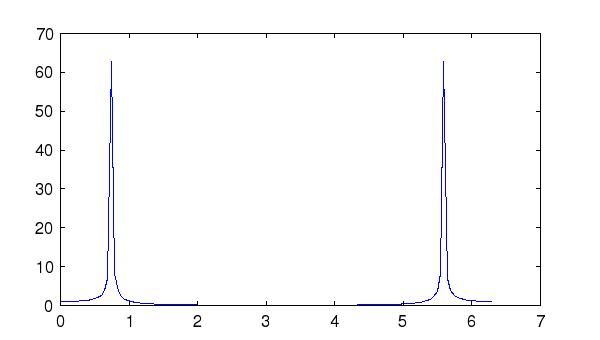
\includegraphics[width=8cm]{fft1}}


The FFT can also be taken along different dimensions, and with padding 
and/or truncation.  The following example demonstrates the Fourier
Transform being computed along each column, and then along each row.
\begin{verbatim}
--> A = [2,5;3,6]

A = 

 2 5 
 3 6 

--> real(fft(A,[],1))

ans = 

  5 11 
 -1 -1 

--> real(fft(A,[],2))

ans = 

  7 -3 
  9 -3 
\end{verbatim}
Fourier transforms can also be padded using the \verb|n| argument.  This
pads the signal with zeros prior to taking the Fourier transform.  Zero
padding in the time domain results in frequency interpolation.  The
following example demonstrates the FFT of a pulse (consisting of 10 ones)
with (red line) and without (green circles) padding.
\begin{verbatim}
--> delta(1:10) = 1;
--> plot((0:255)/256*pi*2,real(fft(delta,256)),'r-');
--> hold on
--> plot((0:9)/10*pi*2,real(fft(delta)),'go');
\end{verbatim}
The resulting plot is:


\centerline{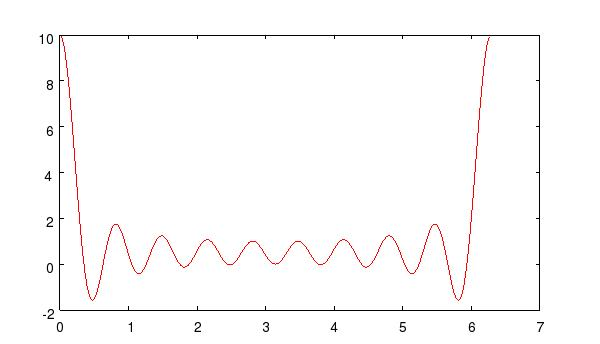
\includegraphics[width=8cm]{fft2}}


\section{FFTN N-Dimensional Forward FFT }

\subsection{Usage}

Computes the DFT of an N-dimensional numerical array along all
dimensions.  The general syntax for its use is
\begin{verbatim}
  y = fftn(x)
\end{verbatim}
which computes the same-size FFTs for each dimension of \verb|x|.
Alternately, you can specify the size vector
\begin{verbatim}
  y = fftn(x,dims)
\end{verbatim}
where \verb|dims| is a vector of sizes.  The array \verb|x| is zero padded
or truncated as necessary in each dimension so that the output
is of size \verb|dims|. The \verb|fftn| function is implemented by a sequence
of calls to \verb|fft|.

\section{FFTSHIFT Shift FFT Output}

\subsection{Usage}

The \verb|fftshift| function shifts the DC component (zero-frequency)
of the output from an FFT to the center of the array.  For vectors
this means swapping the two halves of the vector.  For matrices,
the first and third quadrants are swapped.  So on for N-dimensional
arrays.  The syntax for its use is
\begin{verbatim}
     y = fftshift(x).
\end{verbatim}
Alternately, you can specify that only one dimension be shifted
\begin{verbatim}
     y = fftshift(x,dim).
\end{verbatim}

\section{HILBERT Hilbert Transform}

\subsection{Usage}

The \verb|hilbert| function computes the hilbert transform of the argument
vector or matrix.  The FreeMat \verb|hilbert| function is compatible with
the one from the MATLAB API.  This means that the output of the
\verb|hilbert| function is the sum of the original function and an
imaginary signal containing the Hilbert transform of it.  There are
two syntaxes for the hilbert function.  The first is
\begin{verbatim}
  y = hilbert(x)
\end{verbatim}
where \verb|x| is real vector or matrix.  If \verb|x| is a matrix, then he
Hilbert transform is computed along the columns of \verb|x|.  The
second syntax provides a dimension along which to take the
transform.
\begin{verbatim}
  y = hilbert(x,n)
\end{verbatim}
where \verb|n| is the dimension along which to apply the transformation.

\section{IFFTN N-Dimensional Inverse FFT }

\subsection{Usage}

Computes the inverse DFT of an N-dimensional numerical array along all
dimensions.  The general syntax for its use is
\begin{verbatim}
  y = ifftn(x)
\end{verbatim}
which computes the same-size inverse  FFTs for each dimension of \verb|x|.
Alternately, you can specify the size vector
\begin{verbatim}
  y = ifftn(x,dims)
\end{verbatim}
where \verb|dims| is a vector of sizes.  The array \verb|x| is zero padded
or truncated as necessary in each dimension so that the output
is of size \verb|dims|. The \verb|ifftn| function is implemented by a sequence
of calls to \verb|ifft|.

\section{IFFTSHIFT Inverse Shift FFT Output}

\subsection{Usage}

The \verb|ifftshift| function shifts the DC component (zero-frequency)
of the output from the center of the array back to the first position
and iseffectively the inverse of \verb|fftshift|.  For vectors
this means swapping the two halves of the vector.  For matrices,
the first and third quadrants are swapped.  So on for N-dimensional
arrays.  The syntax for its use is
\begin{verbatim}
     y = ifftshift(x).
\end{verbatim}
Alternately, you can specify that only one dimension be shifted
\begin{verbatim}
     y = ifftshift(x,dim).
\end{verbatim}

\section{INV Invert Matrix}

\subsection{Usage}

Inverts the argument matrix, provided it is square and invertible.
The syntax for its use is
\begin{verbatim}
   y = inv(x)
\end{verbatim}
Internally, the \verb|inv| function uses the matrix divide operators.
For sparse matrices, a sparse matrix solver is used.
\subsection{Example}

Here we invert some simple matrices
\begin{verbatim}
--> a = randi(zeros(3),5*ones(3))

a = 
 5 2 5 
 3 1 1 
 1 4 3 

--> b = inv(a)

b = 
   -0.0294    0.4118   -0.0882 
   -0.2353    0.2941    0.2941 
    0.3235   -0.5294   -0.0294 

--> a*b

ans = 
    1.0000    0.0000   -0.0000 
    0.0000    1.0000    0.0000 
    0.0000    0.0000    1.0000 

--> b*a

ans = 
    1.0000         0    0.0000 
   -0.0000    1.0000   -0.0000 
    0.0000    0.0000    1.0000 
\end{verbatim}

\section{LU LU Decomposition for Matrices}

\subsection{Usage}

Computes the LU decomposition for a matrix.  The form of the
command depends on the type of the argument.  For full (non-sparse)
matrices, the primary form for \verb|lu| is
\begin{verbatim}
   [L,U,P] = lu(A),
\end{verbatim}
where \verb|L| is lower triangular, \verb|U| is upper triangular, and
\verb|P| is a permutation matrix such that \verb|L*U = P*A|.  The second form is
\begin{verbatim}
   [V,U] = lu(A),
\end{verbatim}
where \verb|V| is \verb|P'*L| (a row-permuted lower triangular matrix), 
and \verb|U| is upper triangular.  For sparse, square matrices,
the LU decomposition has the following form:
\begin{verbatim}
   [L,U,P,Q,R] = lu(A),
\end{verbatim}
where \verb|A| is a sparse matrix of either \verb|double| or \verb|dcomplex| type.
The matrices are such that \verb|L*U=P*R*A*Q|, where \verb|L| is a lower triangular
matrix, \verb|U| is upper triangular, \verb|P| and \verb|Q| are permutation vectors
and \verb|R| is a diagonal matrix of row scaling factors.  The decomposition
 is computed using UMFPACK for sparse matrices, and LAPACK for dense
 matrices.
\subsection{Example}

First, we compute the LU decomposition of a dense matrix.
\begin{verbatim}
--> a = float([1,2,3;4,5,8;10,12,3])

a = 
  1  2  3 
  4  5  8 
 10 12  3 

--> [l,u,p] = lu(a)
l = 
    1.0000         0         0 
    0.1000    1.0000         0 
    0.4000    0.2500    1.0000 

u = 
   10.0000   12.0000    3.0000 
         0    0.8000    2.7000 
         0         0    6.1250 

p = 
 0 0 1 
 1 0 0 
 0 1 0 

--> l*u

ans = 
 10 12  3 
  1  2  3 
  4  5  8 

--> p*a

ans = 
 10 12  3 
  1  2  3 
  4  5  8 
\end{verbatim}
Now we repeat the exercise with a sparse matrix, and demonstrate
the use of the permutation vectors.
\begin{verbatim}
--> a = sparse([1,0,0,4;3,2,0,0;0,0,0,1;4,3,2,4])

a = 
 1 1 1
 2 1 3
 4 1 4
 2 2 2
 4 2 3
 4 3 2
 1 4 4
 3 4 1
 4 4 4
--> [l,u,p,q,r] = lu(a)
l = 
 1 1 1
 2 2 1
 3 3 1
 4 4 1
u = 
 1 1 0.153846
 1 2 0.230769
 2 2 0.4
 1 3 0.307692
 2 3 0.6
 3 3 0.2
 1 4 0.307692
 3 4 0.8
 4 4 1
p = 
 4 
 2 
 1 
 3 

q = 
 3 
 2 
 1 
 4 

r = 
 1 1 0.2
 2 2 0.2
 3 3 1
 4 4 0.0769231
--> full(l*a)

ans = 
 1 0 0 4 
 3 2 0 0 
 0 0 0 1 
 4 3 2 4 

--> b = r*a

b = 
 1 1 0.2
 2 1 0.6
 3 1 0
 4 1 0.307692
 1 2 0
 2 2 0.4
 3 2 0
 4 2 0.230769
 1 3 0
 2 3 0
 3 3 0
 4 3 0.153846
 1 4 0.8
 2 4 0
 3 4 1
 4 4 0.307692
--> full(b(p,q))

ans = 
    0.1538    0.2308    0.3077    0.3077 
         0    0.4000    0.6000         0 
         0         0    0.2000    0.8000 
         0         0         0    1.0000 
\end{verbatim}

\section{QR QR Decomposition of a Matrix}

\subsection{Usage}

Computes the QR factorization of a matrix.  The \verb|qr| function has
multiple forms, with and without pivoting.  The non-pivot version
has two forms, a compact version and a full-blown decomposition
version.  The compact version of the decomposition of a matrix 
of size \verb|M x N| is
\begin{verbatim}
  [q,r] = qr(a,0)
\end{verbatim}
where \verb|q| is a matrix of size \verb|M x L| and \verb|r| is a matrix of
size \verb|L x N| and \verb|L = min(N,M)|, and \verb|q*r = a|.  The QR decomposition is
such that the columns of \verb|Q| are orthonormal, and \verb|R| is upper
triangular.  The decomposition is computed using the LAPACK 
routine \verb|xgeqrf|, where \verb|x| is the precision of the matrix.  
FreeMat supports decompositions of \verb|single| and \verb|double| types.

The second form of the non-pivot decomposition omits the second \verb|0|
argument:
\begin{verbatim}
  [q,r] = qr(a)
\end{verbatim}
This second form differs from the previous form only for matrices
with more rows than columns (\verb|M > N|).  For these matrices, the
full decomposition is of a matrix \verb|Q| of size \verb|M x M| and 
a matrix \verb|R| of size \verb|M x N|.  The full decomposition is computed
using the same LAPACK routines as the compact decomposition, but
on an augmented matrix \verb|[a 0]|, where enough columns are added to
form a square matrix.

Generally, the QR decomposition will not return a matrix \verb|R| with
diagonal elements in any specific order.  The remaining two forms 
of the \verb|qr| command utilize permutations of the columns of \verb|a|
so that the diagonal elements of \verb|r| are in decreasing magnitude.
To trigger this form of the decomposition, a third argument is
required, which records the permutation applied to the argument \verb|a|.
The compact version is
\begin{verbatim}
  [q,r,e] = qr(a,0)
\end{verbatim}
where \verb|e| is an integer vector that describes the permutation of
the columns of \verb|a| necessary to reorder the diagonal elements of
\verb|r|.  This result is computed using the LAPACK routines \verb|(s,d)geqp3|.
In the non-compact version of the QR decomposition with pivoting,
\begin{verbatim}
  [q,r,e] = qr(a)
\end{verbatim}
the returned matrix \verb|e| is a permutation matrix, such that 
\verb|q*r*e' = a|.

\section{SVD Singular Value Decomposition of a Matrix}

\subsection{Usage}

Computes the singular value decomposition (SVD) of a matrix.  The 
\verb|svd| function has three forms.  The first returns only the singular
values of the matrix:
\begin{verbatim}
  s = svd(A)
\end{verbatim}
The second form returns both the singular values in a diagonal
matrix \verb|S|, as well as the left and right eigenvectors.
\begin{verbatim}
  [U,S,V] = svd(A)
\end{verbatim}
The third form returns a more compact decomposition, with the
left and right singular vectors corresponding to zero singular
values being eliminated.  The syntax is
\begin{verbatim}
  [U,S,V] = svd(A,0)
\end{verbatim}
\subsection{Function Internals}

Recall that \verb|sigma_i| is a singular value of an \verb|M x N|
matrix \verb|A| if there exists two vectors \verb|u_i, v_i| where \verb|u_i| is
of length \verb|M|, and \verb|v_i| is of length \verb|u_i| and
\[
  A v_i = \sigma_i u_i
\]
and generally
\[
  A = \sum_{i=1}^{K} \sigma_i u_i*v_i',
\]
where \verb|K| is the rank of \verb|A|.  In matrix form, the left singular
vectors \verb|u_i| are stored in the matrix \verb|U| as
\[
  U = [u_1,\ldots,u_m], V = [v_1,\ldots,v_n]
\]
The matrix \verb|S| is then of size \verb|M x N| with the singular
values along the diagonal.  The SVD is computed using the 
\verb|LAPACK| class of functions \verb|GESDD|.
\subsection{Examples}

Here is an example of a partial and complete singular value
decomposition.
\begin{verbatim}
--> A = float(randn(2,3))

A = 

   -0.9542    1.2478   -0.2295 
    0.3075    1.0686   -0.4849 

--> [U,S,V] = svd(A)
U = 

   -0.8410   -0.5411 
   -0.5411    0.8410 

S = 

    1.8058         0         0 
         0    0.8549         0 

V = 

    0.3522    0.9064    0.2331 
   -0.9013    0.2614    0.3454 
    0.2521   -0.3317    0.9091 

--> U*S*V'

ans = 

   -0.9542    1.2478   -0.2295 
    0.3075    1.0686   -0.4849 

--> svd(A)

ans = 

    1.8058 
    0.8549 
\end{verbatim}

\chapter{Signal Processing Functions}
\section{CONV Convolution Function}

\subsection{Usage}

The \verb|conv| function performs a one-dimensional convolution of two
vector arguments.  The syntax for its use is
\begin{verbatim}
     z = conv(x,y)
\end{verbatim}
where \verb|x| and \verb|y| are vectors.  The output is of length \verb|nx + ny -1|.
The \verb|conv| function calls \verb|conv2| to do the calculation.  See its
help for more details.

\section{CONV2 Matrix Convolution}

\subsection{Usage}

The \verb|conv2| function performs a two-dimensional convolution of
matrix arguments.  The syntax for its use is
\begin{verbatim}
    Z = conv2(X,Y)
\end{verbatim}
which performs the full 2-D convolution of \verb|X| and \verb|Y|.  If the 
input matrices are of size \verb|[xm,xn]| and \verb|[ym,yn]| respectively,
then the output is of size \verb|[xm+ym-1,xn+yn-1]|.  Another form is
\begin{verbatim}
    Z = conv2(hcol,hrow,X)
\end{verbatim}
where \verb|hcol| and \verb|hrow| are vectors.  In this form, \verb|conv2|
first convolves \verb|Y| along the columns with \verb|hcol|, and then 
convolves \verb|Y| along the rows with \verb|hrow|.  This is equivalent
to \verb|conv2(hcol(:)*hrow(:)',Y)|.

You can also provide an optional \verb|shape| argument to \verb|conv2|
via either
\begin{verbatim}
    Z = conv2(X,Y,'shape')
    Z = conv2(hcol,hrow,X,'shape')
\end{verbatim}
where \verb|shape| is one of the following strings
\begin{itemize}
\item  \verb|'full'| - compute the full convolution result - this is the default if no \verb|shape| argument is provided.

\item  \verb|'same'| - returns the central part of the result that is the same size as \verb|X|.

\item  \verb|'valid'| - returns the portion of the convolution that is computed without the zero-padded edges.  In this situation, \verb|Z| has 
size \verb|[xm-ym+1,xn-yn+1]| when \verb|xm>=ym| and \verb|xn>=yn|.  Otherwise
\verb|conv2| returns an empty matrix.

\end{itemize}
\subsection{Function Internals}

The convolution is computed explicitly using the definition:
\[
  Z(m,n) = \sum_{k} \sum_{j} X(k,j) Y(m-k,n-j)
\]
If the full output is requested, then \verb|m| ranges over \verb|0 <= m < xm+ym-1|
and \verb|n| ranges over \verb|0 <= n < xn+yn-1|.  For the case where \verb|shape|
is \verb|'same'|, the output ranges over \verb|(ym-1)/2 <= m < xm + (ym-1)/2|
and \verb|(yn-1)/2 <= n < xn + (yn-1)/2|.

\chapter{Numerical Methods}
\section{ODE45 Numerical Solution of ODEs}

\subsection{Usage}

 function [t,y] = ode45(f,tspan,y0,options,varargin)
 function SOL   = ode45(f,tspan,y0,options,varargin)

 ode45 is a solver for ordinary differential equations and initial value problems.
 To solve the ODE
\begin{verbatim}
      y'(t) =  f(t,y)
      y(0)  =  y0
\end{verbatim}
 over the interval tspan=[t0 t1], you can use ode45. For example, to solve
 the ode

      y'   =  y
      y(0) =  1

 whose exact solution is y(t)=exp(t), over the interval t0=0, t1=3, do
@>
 If you want a dense output (i.e., an output that also contains an interpolating
 spline), use instead
@>
 You can view the result using
\begin{verbatim}
      plot(0:0.01:3,deval(SOL,0:0.01:3))
\end{verbatim}
 You will notice that this function is available for "every" value of t, while

      plot(t,y,'o-')

 is only available at a few points.

 The optional argument 'options' is a structure. It may contain any of the
 following fields:

 'AbsTol'      - Absolute tolerance, default is 1e-6.
 'RelTol'      - Relative tolerance, default is 1e-3.
 'MaxStep'     - Maximum step size, default is (tspan(2)-tspan(1))/10
 'InitialStep' - Initial step size, default is maxstep/100
 'Stepper'     - To override the default Fehlberg integrator
 'Events'      - To provide an event function
 'Projection'  - To provide a projection function

 The varargin is ignored by this function, but is passed to all your callbacks, i.e.,
 f, the event function and the projection function.

 ==Event Function==

 The event function can be used to detect situations where the integrator should stop,
 possibly because the right-hand-side has changed, because of a collision, etc...

 An event function should look like

    function [val,isterminal,direction]=event(t,y,...)

 The return values are:

 val        - the value of the event function.
 isterminal - whether or not this event should cause termination of the integrator.
 direction  - 1=upcrossings only matter, -1=downcrossings only, 0=both.

 == Projection function ==

 For geometric integration, you can provide a projection function which will be
 called after each time step. The projection function has the following signature:

     function yn=project(t,yn,...);

 If the output yn is very different from the input yn, the quality of interpolation
 may decrease.

\chapter{Operating System Functions}
\section{CD Change Working Directory Function}

\subsection{Usage}

Changes the current working directory to the one specified as the argument.  The general syntax for its use is
\begin{verbatim}
  cd('dirname')
\end{verbatim}
but this can also be expressed as
\begin{verbatim}
  cd 'dirname'
\end{verbatim}
or 
\begin{verbatim}
  cd dirname
\end{verbatim}
Examples of all three usages are given below.
Generally speaking, \verb|dirname| is any string that would be accepted 
by the underlying OS as a valid directory name.  For example, on most 
systems, \verb|'.'| refers to the current directory, and \verb|'..'| refers 
to the parent directory.  Also, depending on the OS, it may be necessary 
to ``escape'' the directory seperators.  In particular, if directories 
are seperated with the backwards-slash character \verb|'\\'|, then the 
path specification must use double-slashes \verb|'\\\\'|. Note: to get 
file-name completion to work at this time, you must use one of the 
first two forms of the command.

\subsection{Example}

The \verb|pwd| command returns the current directory location.  First, 
we use the simplest form of the \verb|cd| command, in which the directory 
name argument is given unquoted.
\begin{verbatim}
--> pwd

ans = 
/home/sbasu/Devel/FreeMat/help/tmp
--> cd ..
--> pwd

ans = 
/home/sbasu/Devel/FreeMat/help
\end{verbatim}
Next, we use the ``traditional'' form of the function call, using 
both the parenthesis and a variable to store the quoted string.
\begin{verbatim}
--> a = pwd;
--> cd(a)
--> pwd

ans = 
/home/sbasu/Devel/FreeMat/help/tmp
\end{verbatim}

\section{COPYFILE Copy Files}

\subsection{Usage}

Copies a file or files from one location to another.  There are 
several syntaxes for this function that are acceptable:
\begin{verbatim}
   copyfile(file_in,file_out)
\end{verbatim}
copies the file from \verb|file\_in| to \verb|file\_out|.  Also, the second
argument can be a directory name:
\begin{verbatim}
   copyfile(file_in,directory_out)
\end{verbatim}
in which case \verb|file\_in| is copied into the directory specified by
\verb|directory\_out|.  You can also use \verb|copyfile| to copy entire directories
as in
\begin{verbatim}
   copyfile(dir_in,dir_out)
\end{verbatim}
in which case the directory contents are copied to the destination directory
(which is created if necessary).  Finally, the first argument to \verb|copyfile| can
contain wildcards
\begin{verbatim}
   copyfile(pattern,directory_out)
\end{verbatim}
in which case all files that match the given pattern are copied to the output
directory.   Note that to remain compatible with the MATLAB API, this function
will delete/replace destination files that already exist, unless they are marked
as read-only.  If you want to force the copy to succeed, you can append a \verb|'f'|
argument to the \verb|copyfile| function:
\begin{verbatim}
   copyfile(arg1,arg2,'f')
\end{verbatim}
or equivalently
\begin{verbatim}
   copyfile arg1 arg2 f
\end{verbatim}

\section{DELETE Delete a File}

\subsection{Usage}

Deletes a file.  The general syntax for its use is
\begin{verbatim}
  delete('filename')
\end{verbatim}
or alternately
\begin{verbatim}
  delete filename
\end{verbatim}
which removes the file described by \verb|filename| which must
be relative to the current path.

\section{DIR List Files Function}

\subsection{Usage}

In some versions of FreeMat (pre 3.1), the \verb|dir| function was aliased
to the \verb|ls| function.  Starting with version \verb|3.1|, the \verb|dir| function
has been rewritten to provide compatibility with MATLAB.  The general syntax
for its use is
\begin{verbatim}
  dir
\end{verbatim}
in which case, a listing of the files in the current directory are output to the
console.  Alternately, you can specify a target via
\begin{verbatim}
  dir('name')
\end{verbatim}
or using the string syntax
\begin{verbatim}
  dir name
\end{verbatim}
If you want to capture the output of the \verb|dir| command, you can assign the output
to an array
\begin{verbatim}
  result = dir('name')
\end{verbatim}
(or you can omit \verb|'name'| to get a directory listing of the current directory.  The
resulting array \verb|result| is a structure array containing the fields:
\begin{itemize}
\item  \verb|name| the filename as a string

\item  \verb|date| the modification date and time stamp as a string

\item  \verb|bytes| the size of the file in bytes as a \verb|uint64|

\item  \verb|isdir| a logical that is \verb|1| if the file corresponds to a directory.

\end{itemize}
Note that \verb|'name'| can also contain wildcards (e.g., \verb|dir *.m| to get a listing of
all FreeMat scripts in the current directory.

\section{DIRSEP Director Seperator}

\subsection{Usage}

Returns the directory seperator character for the current platform.  The 
general syntax for its use is
\begin{verbatim}
   y = dirsep
\end{verbatim}
This function can be used to build up paths (or see \verb|fullfile| for another
way to do this.

\section{FILEPARTS Extract Filename Parts}

\subsection{Usage}

The \verb|fileparts| takes a filename, and returns the path, filename, extension, and
(for MATLAB-compatibility) an empty version number of the file.  The syntax for its use is
\begin{verbatim}
    [path,name,extension,version] = fileparts(filename)
\end{verbatim}
where \verb|filename| is a string containing the description of the file, and \verb|path|
is the \verb|path| to the file, 

\section{FULLFILE Build a Full Filename From Pieces}

\subsection{Usage}

The \verb|fullfile| routine constructs a full filename from a set of
pieces, namely, directory names and a filename.  The syntax is:
\begin{verbatim}
  x = fullfile(dir1,dir2,...,dirn,filename)
\end{verbatim}
where each of the arguments are strings.  The \verb|fullfile| function
is equivalent to \verb|[dir1 dirsep dir2 dirsep ... dirn dirsep filename]|.
\subsection{Example}

\begin{verbatim}
--> fullfile('path','to','my','file.m')

ans = 
path/to/my/file.m
\end{verbatim}

\section{GETPATH Get Current Search Path}

\subsection{Usage}

Returns a \verb|string| containing the current FreeMat search path.  The general syntax for
its use is
\begin{verbatim}
  y = getpath
\end{verbatim}
The delimiter between the paths depends on the system being used.  For Win32, the
delimiter is a semicolon.  For all other systems, the delimiter is a colon.

\subsection{Example}

The \verb|getpath| function is straightforward.
\begin{verbatim}
--> getpath

ans = 
/home/sbasu/Devel/FreeMat4
\end{verbatim}

\section{LS List Files Function}

\subsection{Usage}

Lists the files in a directory or directories.  The general syntax for its use is
\begin{verbatim}
  ls('dirname1','dirname2',...,'dirnameN')
\end{verbatim}
but this can also be expressed as
\begin{verbatim}
  ls 'dirname1' 'dirname2' ... 'dirnameN'
\end{verbatim}
or 
\begin{verbatim}
  ls dirname1 dirname2 ... dirnameN
\end{verbatim}
For compatibility with some environments, the function \verb|dir| can also be used instead of \verb|ls|.  Generally speaking, \verb|dirname| is any string that would be accepted by the underlying OS as a valid directory name.  For example, on most systems, \verb|'.'| refers to the current directory, and \verb|'..'| refers to the parent directory.  Also, depending on the OS, it may be necessary to ``escape'' the directory seperators.  In particular, if directories are seperated with the backwards-slash character \verb|'\\'|, then the path specification must use double-slashes \verb|'\\\\'|. Two points worth mentioning about the \verb|ls| function:
\begin{itemize}
\item  To get file-name completion to work at this time, you must use one of the first two forms of the command.

\item  If you want to capture the output of the \verb|ls| command, use the \verb|system| function instead.

\end{itemize}

\subsection{Example}

First, we use the simplest form of the \verb|ls| command, in which the directory name argument is given unquoted.
@>
Next, we use the ``traditional'' form of the function call, using both the parenthesis and the quoted string.
@>
In the third version, we use only the quoted string argument without parenthesis.  
@>

\section{MKDIR Make Directory}

\subsection{Usage}

Creates a directory.  The general syntax for its use is
\begin{verbatim}
  mkdir('dirname')
\end{verbatim}
which creates the directory \verb|dirname| if it does not exist.  The argument
\verb|dirname| can be either a relative path or an absolute path.  For compatibility
with MATLAB, the following syntax is also allowed
\begin{verbatim}
  mkdir('parentdir','dirname')
\end{verbatim}
which attempts to create a directory \verb|dirname| in the directory given by \verb|parentdir|.
However, this simply calls \verb|mkdir([parentdir dirsep dirname])|, and if this is not
the required behavior, please file an enhancement request to have it changed.  Note that
\verb|mkdir| returns a logical \verb|1| if the call succeeded, and a logical \verb|0| if not.

\section{PWD Print Working Directory Function}

\subsection{Usage}

Returns a \verb|string| describing the current working directory.  The general syntax for its use is
\begin{verbatim}
  y = pwd
\end{verbatim}

\subsection{Example}

The \verb|pwd| function is fairly straightforward.
\begin{verbatim}
--> pwd

ans = 
/home/basu/dev/branches/FreeMat4/help/tmp
\end{verbatim}

\section{RMDIR Remove Directory}

\subsection{Usage}

Deletes a directory.  The general syntax for its use is
\begin{verbatim}
  rmdir('dirname')
\end{verbatim}
which removes the directory \verb|dirname| if it is empty.  If you
want to delete the directory and all subdirectories and files
in it, use the syntax
\begin{verbatim}
  rmdir('dirname','s')
\end{verbatim}

\section{SETPATH Set Current Search Path}

\subsection{Usage}

Changes the current FreeMat search path.  The general syntax for
its use is
\begin{verbatim}
  setpath(y)
\end{verbatim}
where \verb|y| is a \verb|string| containing a delimited list of directories
to be searched for M files and libraries.  
The delimiter between the paths depends on the system being used.  For Win32, the
delimiter is a semicolon.  For all other systems, the delimiter is a colon.

@Example
The \verb|setpath| function is straightforward.
@>

\section{SYSTEM Call an External Program}

\subsection{Usage}

The \verb|system| function allows you to call an external
program from within FreeMat, and capture the output.
The syntax of the \verb|system| function is
\begin{verbatim}
  y = system(cmd)
\end{verbatim}
where \verb|cmd| is the command to execute.  The return
array \verb|y| is of type \verb|cell-array|, where each entry
in the array corresponds to a line from the output.
\subsection{Example}

Here is an example of calling the \verb|ls| function (the
list files function under Un*x-like operating system).
\begin{verbatim}
--> y = system('ls')

y = 

 Columns 1 to 3

 [chain1.m] [chain2.m] [chain3.m] 

 Columns 4 to 6

 [conv2_eqn1.png] [conv2_eqn.aux] [conv2_eqn.dvi] 

 Columns 7 to 9

 [conv2_eqn.log] [conv2_eqn.tex] [cumprod_eqn1.png] 

 Columns 10 to 12

 [cumprod_eqn.aux] [cumprod_eqn.dvi] [cumprod_eqn.log] 

 Columns 13 to 15

 [cumprod_eqn.tex] [cumsum_eqn1.png] [cumsum_eqn.aux] 

 Columns 16 to 18

 [cumsum_eqn.dvi] [cumsum_eqn.log] [cumsum_eqn.tex] 

 Columns 19 to 21

 [do_jit_test.m] [eig_eqn1.png] [eig_eqn2.png] 

 Columns 22 to 24

 [eig_eqn3.png] [eig_eqn4.png] [eig_eqn5.png] 

 Columns 25 to 27

 [eig_eqn6.png] [eig_eqn.aux] [eig_eqn.dvi] 

 Columns 28 to 30

 [eig_eqn.log] [eig_eqn.tex] [evenoddtest.m] 

 Columns 31 to 33

 [fft1.jpg] [fft1.png] [fft2.jpg] 

 Columns 34 to 36

 [fft2.png] [fft_eqn1.png] [fft_eqn2.png] 

 Columns 37 to 39

 [fft_eqn3.png] [fft_eqn4.png] [fft_eqn.aux] 

 Columns 40 to 42

 [fft_eqn.dvi] [fft_eqn.log] [fft_eqn.tex] 

 Columns 43 to 45

 [find_eqn1.png] [find_eqn.aux] [find_eqn.dvi] 

 Columns 46 to 48

 [find_eqn.log] [find_eqn.tex] [jit_test001.m] 

 Columns 49 to 51

 [jit_test002.m] [jit_test003.m] [jit_test004.m] 

 Columns 52 to 54

 [jit_test005.m] [jit_test006.m] [jit_test007.m] 

 Columns 55 to 57

 [jit_test008.m] [jit_test009.m] [jit_test010.m] 

 Columns 58 to 60

 [jit_test011.m] [jit_test012.m] [jit_test013.m] 

 Columns 61 to 63

 [jit_test014.m] [jit_test015.m] [jit_test016.m] 

 Columns 64 to 66

 [jit_test017.m] [jit_test018.m] [jit_test019.m] 

 Columns 67 to 69

 [jit_test020.m] [jit_test021.m] [jit_test022.m] 

 Columns 70 to 72

 [jit_test023.m] [jit_test024.m] [loadsave.dat] 

 Columns 73 to 75

 [max_eqn1.png] [max_eqn2.png] [max_eqn3.png] 

 Columns 76 to 78

 [max_eqn.aux] [max_eqn.dvi] [max_eqn.log] 

 Columns 79 to 81

 [max_eqn.tex] [mean_eqn1.png] [mean_eqn.aux] 

 Columns 82 to 84

 [mean_eqn.dvi] [mean_eqn.log] [mean_eqn.tex] 

 Columns 85 to 87

 [min_eqn1.png] [min_eqn2.png] [min_eqn3.png] 

 Columns 88 to 90

 [min_eqn.aux] [min_eqn.dvi] [min_eqn.log] 

 Columns 91 to 93

 [min_eqn.tex] [nargintest.m] [nargouttest.m] 

 Columns 94 to 96

 [source_test] [source_test_script.m] [test_assignin1.m] 

 Columns 97 to 99

 [test_assignin2.m] [test_bin2int1.m] [test_bitand1.m] 

 Columns 100 to 102

 [test_bitor1.m] [test_bitxor1.m] [test.bmp] 

 Columns 103 to 105

 [test_builtin1.m] [test_cell1.m] [test_clear1.m] 

 Columns 106 to 108

 [test_clear2.m] [test_conv2_1.m] [test_ctype1.m] 

 Columns 109 to 111

 [test.dat] [test_dcomplex1.m] [test_diag1.m] 

 Columns 112 to 114

 [test_diag2.m] [test_diag3.m] [test_diag4.m] 

 Columns 115 to 117

 [test_diag5.m] [test_dlmread1.m] [test_eig1.m] 

 Columns 118 to 120

 [test_eig2.m] [test_eig3.m] [test_eig4.m] 

 Columns 121 to 123

 [test_eig5.m] [test_eig6.m] [test_empty.m] 

 Columns 124 to 126

 [test_eps1.m] [test_error1.m] [test_eval1.m] 

 Columns 127 to 129

 [test_eval2.m] [test_eval3.m] [test_evalin1.m] 

 Columns 130 to 132

 [test_evalin2.m] [test_exist1.m] [test_exist2.m] 

 Columns 133 to 135

 [test_feval1.m] [test_fieldnames1.m] [test_imwrite_imread.m] 

 Columns 136 to 138

 [test_int2bin1.m] [test_isset1.m] [test_jit.m] 

 Columns 139 to 141

 [test_lasterr1.m] [test_load1.m] [test_lu1.m] 

 Columns 142 to 144

 [test_lu2.m] [test_nargin1.m] [test_nargin2.m] 

 Columns 145 to 147

 [test_permute1.m] [test_permute2.m] [test_repmat1.m] 

 Columns 148 to 150

 [test_repmat2.m] [test_repmat3.m] [test_save1.m] 

 Columns 151 to 153

 [test_source.m] [test_sparse20.m] [test_sparse21.m] 

 Columns 154 to 156

 [test_sparse45.m] [test_sparse58.m] [test_sparse68.m] 

 Columns 157 to 159

 [test_sparse70.m] [test_sparse74.m] [test_sparse75.m] 

 Columns 160 to 162

 [testtext] [test_typeof1.m] [test_typeof2.m] 

 Columns 163 to 165

 [test_typeof3.m] [test_typeof4.m] [test_typeof5.m] 

 Columns 166 to 167

 [test_typeof6.m] [test_uint64_1.m] 

--> y{1}

ans = 
chain1.m
\end{verbatim}

\chapter{Optimization and Curve Fitting}
\section{FITFUN Fit a Function}

\subsection{Usage}

Fits \verb|n| (non-linear) functions of \verb|m| variables using least squares
and the Levenberg-Marquardt algorithm.  The general syntax for its usage
is
\begin{verbatim}
  [xopt,yopt] = fitfun(fcn,xinit,y,weights,tol,params...)
\end{verbatim}
Where \verb|fcn| is the name of the function to be fit, \verb|xinit| is the
initial guess for the solution (required), \verb|y| is the right hand side,
i.e., the vector \verb|y| such that:
\[
   xopt = \arg \min_{x} \|\mathrm{diag}(weights)*(f(x) - y)\|_2^2,
\]
the output \verb|yopt| is the function \verb|fcn| evaluated at \verb|xopt|.  
The vector \verb|weights| must be the same size as \verb|y|, and contains the
relative weight to assign to an error in each output value.  Generally,
the ith weight should reflect your confidence in the ith measurement.
The parameter \verb|tol| is the tolerance used for convergence.
The function \verb|fcn| must return a vector of the same size as \verb|y|,
and \verb|params| are passed to \verb|fcn| after the argument \verb|x|, i.e.,
\[
  y = fcn(x,param1,param2,...).
\]
Note that both \verb|x| and \verb|y| (and the output of the function) must all
be real variables.  Complex variables are not handled yet.

\section{GAUSFIT Gaussian Curve Fit}

\subsection{Usage}

The \verb|gausfit| routine has the following syntax
\begin{verbatim}
  [mu,sigma,dc,gain,yhat] = gausfit(t,y,w,mug,sigmag,dcg,gaing).
\end{verbatim}
where the required inputs are
\begin{itemize}
\item  \verb|t| - the values of the independant variable (e.g., time samples)

\item  \verb|y| - the values of the dependant variable (e.g., f(t))

\end{itemize}
The following inputs are all optional, and default values are
available for each of them.
\begin{itemize}
\item  \verb|w| - the weights to use in the fitting (set to ones if omitted)

\item  \verb|mug| - initial estimate of the mean

\item  \verb|sigmag| - initial estimate of the sigma (standard deviation)

\item  \verb|dcg| - initial estimate of the DC value

\item  \verb|gaing| - initial estimate of the gain

\end{itemize}
The fit is of the form \verb|yhat=gain*exp((t-mu).^2/(2*sigma^2))+dc|.
The outputs are 
\begin{itemize}
\item  \verb|mu| - the mean of the fit

\item  \verb|sigma| - the sigma of the fit

\item  \verb|dc| - the dc term of the fit

\item  \verb|gain| - the gain of the gaussian fit

\item  \verb|yhat| - the output samples (the Gaussian fits)

\end{itemize}
Because the fit is nonlinear, a good initial guess is critical to
convergence of the solution.  Thus, you can supply initial guesses
for each of the parameters using the \verb|mug|, \verb|sigmag|, \verb|dcg|, 
\verb|gaing| arguments.  Any arguments not supplied are estimated using 
a simple algorithm. In particular, the DC value is estimated by 
taking the minimum value  from the vector \verb|y|.  The gain is 
estimated from the range of \verb|y|.  The mean and standard deviation 
are estimated using the first and second order moments of \verb|y|.
This function uses \verb|fitfun|.
\subsection{Example}

Suppose we want to fit a cycle of a cosine using a Gaussian shape.
@>
Which results in the following plot


\centerline{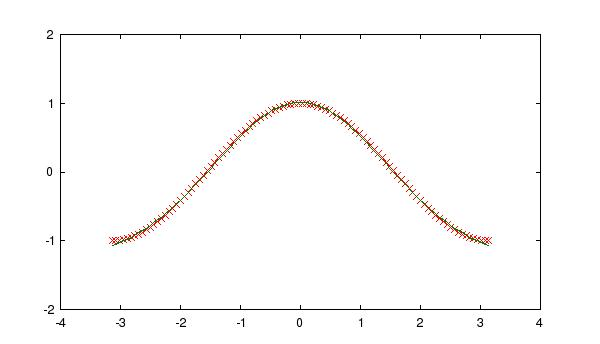
\includegraphics[width=8cm]{gausfit1}}


\section{INTERPLIN1 Linear 1-D Interpolation}

\subsection{Usage}

Given a set of monotonically increasing \verb|x| coordinates and a 
corresponding set of \verb|y| values, performs simple linear 
interpolation to a new set of \verb|x| coordinates. The general syntax
for its usage is
\begin{verbatim}
   yi = interplin1(x1,y1,xi)
\end{verbatim}
where \verb|x1| and \verb|y1| are vectors of the same length, and the entries
in \verb|x1| are monotoniccally increasing.  The output vector \verb|yi| is
the same size as the input vector \verb|xi|.  For each element of \verb|xi|,
the values in \verb|y1| are linearly interpolated.  For values in \verb|xi| 
that are outside the range of \verb|x1| the default value returned is
\verb|nan|.  To change this behavior, you can specify the extrapolation
flag:
\begin{verbatim}
   yi = interplin1(x1,y1,xi,extrapflag)
\end{verbatim}
Valid options for \verb|extrapflag| are:
\begin{itemize}
\item  \verb|'nan'| - extrapolated values are tagged with \verb|nan|s

\item  \verb|'zero'| - extrapolated values are set to zero

\item  \verb|'endpoint'| - extrapolated values are set to the endpoint values 

\item  \verb|'extrap'| - linear extrapolation is performed

\end{itemize}
The \verb|x1| and \verb|xi| vectors must be real, although complex types
are allowed for \verb|y1|.
\subsection{Example}

Here is an example of simple linear interpolation with the different
extrapolation modes.  We start with a fairly coarse sampling of a 
cosine.
\begin{verbatim}
--> x = linspace(-pi*7/8,pi*7/8,15);
--> y = cos(x);
--> plot(x,y,'ro');
\end{verbatim}
which is shown here


\centerline{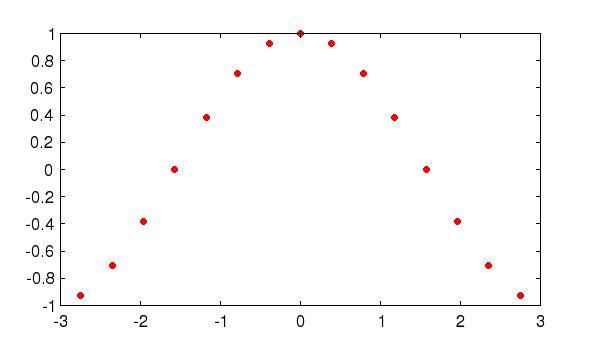
\includegraphics[width=8cm]{interplin1_1}}

Next, we generate a finer sampling over a slightly broader range
(in this case \verb|[-pi,pi]|).  First, we demonstrate the \verb|'nan'| 
extrapolation method
\begin{verbatim}
--> xi = linspace(-4,4,100);
--> yi_nan = interplin1(x,y,xi,'nan');
--> yi_zero = interplin1(x,y,xi,'zero');
--> yi_endpoint = interplin1(x,y,xi,'endpoint');
--> yi_extrap = interplin1(x,y,xi,'extrap');
--> plot(x,y,'ro',xi,yi_nan,'g-x',xi,yi_zero,'g-x',xi,yi_endpoint,'g-x',xi,yi_extrap,'g-x');
\end{verbatim}
which is shown here


\centerline{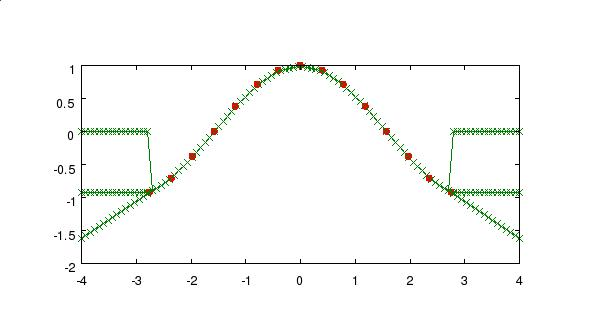
\includegraphics[width=8cm]{interplin1_2}}


\section{POLY Convert Roots To Polynomial Coefficients}

\subsection{Usage}

This function calculates the polynomial coefficients for given roots
\begin{verbatim}
    p = poly(r)
\end{verbatim}
when \verb|r| is a vector, is a vector whose elements are the coefficients 
of the polynomial whose roots are the elements of \verb|r|.  Alternately,
you can provide a matrix
\begin{verbatim}
    p = poly(A)
\end{verbatim}
when \verb|A| is an \verb|N x N| square matrix, is a row vector with 
\verb|N+1| elements which are the coefficients of the
characteristic polynomial, \verb|det(lambda*eye(size(A))-A)|.

Contributed by Paulo Xavier Candeias under GPL.
\subsection{Example}

Here are some examples of the use of \verb|poly|
\begin{verbatim}
--> A = [1,2,3;4,5,6;7,8,0]

A = 

 1 2 3 
 4 5 6 
 7 8 0 

--> p = poly(A)

p = 

    1.0000   -6.0000  -72.0000  -27.0000 

--> r = roots(p)

r = 

   12.1229 
   -5.7345 
   -0.3884 
\end{verbatim}

\section{POLYDER Polynomial Coefficient Differentiation}

\subsection{Usage}

The \verb|polyder| function returns the polynomial coefficients resulting
from differentiation of polynomial \verb|p|. The syntax for its use is either
\begin{verbatim}
 pder = polyder(p)
\end{verbatim}
 for the derivitave of polynomial p, or
\begin{verbatim}
 convp1p2der = polyder(p1,p2)
\end{verbatim}
 for the derivitave of polynomial conv(p1,p2), or still
\begin{verbatim}
 [nder,dder] = polyder(n,d)
\end{verbatim}
for the derivative of polynomial \verb|n/d| (\verb|nder| is the numerator
and \verb|dder| is the denominator). In all cases the polynomial 
coefficients are assumed to be in decreasing degree.
Contributed by Paulo Xavier Candeias under GPL
\subsection{Example}

Here are some examples of the use of \verb|polyder|
@>
@>
@>

\section{POLYFIT Fit Polynomial To Data}

\subsection{Usage}

The \verb|polyfit| routine has the following syntax
\begin{verbatim}
  p = polyfit(x,y,n)
\end{verbatim}
where \verb|x| and \verb|y| are vectors of the same size, and
\verb|n| is the degree of the approximating polynomial.  
The resulting vector \verb|p| forms the coefficients of
the optimal polynomial (in descending degree) that fit
\verb|y| with \verb|x|.  
\subsection{Function Internals}

The \verb|polyfit| routine finds the approximating polynomial
\[
   p(x) = p_1 x^n + p_2 x^{n-1} + \dots + p_n x + p_{n+1}
\]
such that
\[
   \sum_{i} (p(x_i) - y_i)^2
\]
is minimized.  It does so by forming the Vandermonde matrix
and solving the resulting set of equations using the backslash
operator.  Note that the Vandermonde matrix can become poorly
conditioned with large \verb|n| quite rapidly.
\subsection{Example}

A classic example from Edwards and Penny, consider the problem
of approximating a sinusoid with a polynomial.  We start with
a vector of points evenly spaced on the unit interval, along with
a vector of the sine of these points.
\begin{verbatim}
--> x = linspace(0,1,20);
--> y = sin(2*pi*x);
--> plot(x,y,'r-')
\end{verbatim}
The resulting plot is shown here


\centerline{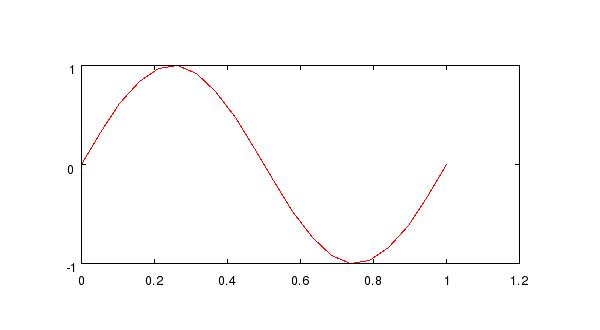
\includegraphics[width=8cm]{polyfit1}}

Next, we fit a third degree polynomial to the sine, and use
\verb|polyval| to plot it
\begin{verbatim}
--> p = polyfit(x,y,3)

p = 

   21.9170  -32.8756   11.1897   -0.1156 

--> f = polyval(p,x);
--> plot(x,y,'r-',x,f,'ko');
\end{verbatim}
The resulting plot is shown here


\centerline{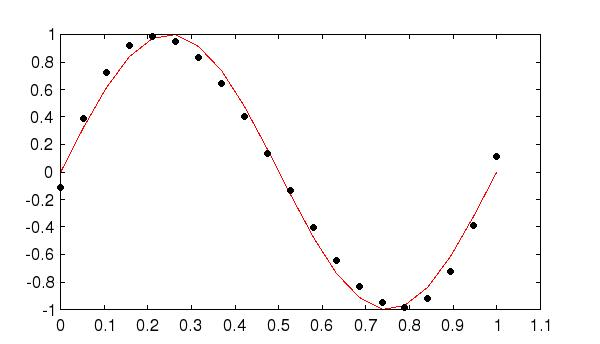
\includegraphics[width=8cm]{polyfit2}}

Increasing the order improves the fit, as
\begin{verbatim}
--> p = polyfit(x,y,11)

p = 
 
Columns 1 to 9

   12.4644  -68.5541  130.0555  -71.0940  -38.2814  -14.1222   85.1018   -0.5642  -41.2861 
 
Columns 10 to 12

   -0.0029    6.2832   -0.0000 

--> f = polyval(p,x);
--> plot(x,y,'r-',x,f,'ko');
\end{verbatim}
The resulting plot is shown here


\centerline{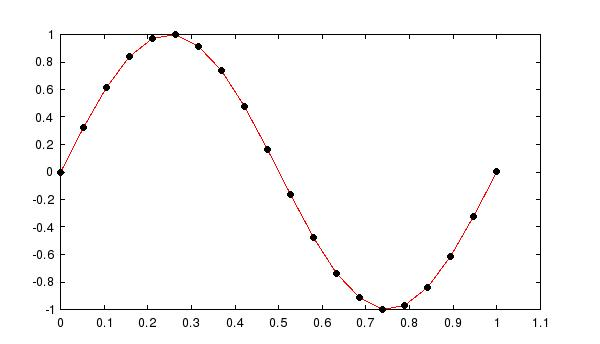
\includegraphics[width=8cm]{polyfit3}}


\section{POLYINT Polynomial Coefficient Integration}

\subsection{Usage}

 The polyint function returns the polynomial coefficients resulting
 from integration of polynomial p. The syntax for its use is either
\begin{verbatim}
 pint = polyint(p,k)
\end{verbatim}
 or, for a default \verb|k = 0|,
\begin{verbatim}
 pint = polyint(p);
\end{verbatim}
 where \verb|p| is a vector of polynomial coefficients assumed to be in
 decreasing degree and \verb|k| is the integration constant.
 Contributed by Paulo Xavier Candeias under GPL
\subsection{Example}

Here is are some examples of the use of \verb|polyint|.
\begin{verbatim}
--> polyint([2,3,4])

ans = 

    0.6667    1.5000    4.0000         0 
\end{verbatim}
And
\begin{verbatim}
--> polyint([2,3,4],5)

ans = 

    0.6667    1.5000    4.0000    5.0000 
\end{verbatim}

\section{POLYVAL Evaluate Polynomial Fit at Selected Points}

\subsection{Usage}

The \verb|polyval| routine has the following syntax
\begin{verbatim}
  y = polyval(p,x)
\end{verbatim}
where \verb|p| is a vector of polynomial coefficients,
in decreasing degree (as generated by \verb|polyfit|, for example).
If \verb|x| is a matrix, the polynomial is evaluated in the matrix
sense (in which case \verb|x| must be square).
\subsection{Function Internals}

The polynomial is evaluated using a recursion method.  If the
polynomial is
\[
   p(x) = p_1 x^n + p_2 x^{n-1} + \dots + p_n x + p_{n+1}
\]
then the calculation is performed as
\[
   p(x) = ((p_1) x + p_2) x + p_3
\]
\subsection{Example}

Here is a plot of \verb|x\^3| generated using polyval
\begin{verbatim}
--> p = [1 0 0 0]

p = 
 1 0 0 0 

--> x = linspace(-1,1);
--> y = polyval(p,x);
--> plot(x,y,'r-')
\end{verbatim}
Here is the resulting plot


\centerline{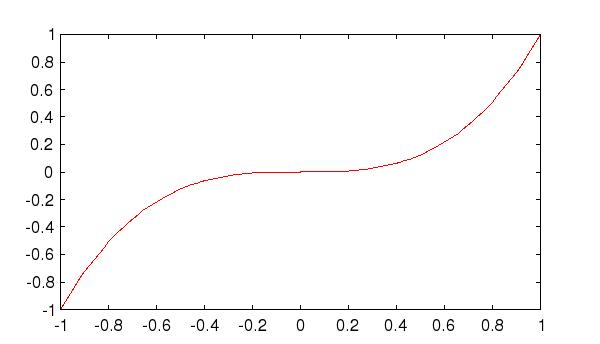
\includegraphics[width=8cm]{polyval1}}


\section{ROOTS Find Roots of Polynomial}

\subsection{Usage}

The \verb|roots| routine will return a column vector containing the
roots of a polynomial.  The general syntax is
\begin{verbatim}
   z = roots(p)
\end{verbatim}
where \verb|p| is a vector containing the coefficients of the polynomial
ordered in descending powers.  
\subsection{Function Internals}

Given a vector 
\[
   [p_1, p_2, \dots p_n]
\]
which describes a polynomial
\[
   p_1 x^{n-1} + p_2 x^{n-2} + \dots + p_n
\]
we construct the companion matrix (which has a characteristic polynomial
matching the polynomial described by \verb|p|), and then find the eigenvalues
of it (which are the roots of its characteristic polynomial), and
which are also the roots of the polynomial of interest.  This technique
for finding the roots is described in the help page for \verb|roots| on the Mathworks
website.
\subsection{Example}

Here is an example of finding the roots to the polynomial
\[
   x^3 - 6x^2 - 72x - 27
\]
@>

\chapter{Handle-Based Graphics}
\section{AXES Create Handle Axes}

\subsection{Usage}

This function has three different syntaxes.  The first takes
no arguments,
\begin{verbatim}
  h = axes
\end{verbatim}
and creates a new set of axes that are parented to the current
figure (see \verb|gcf|).  The newly created axes are made the current
axes (see \verb|gca|) and are added to the end of the list of children 
for the current figure.
The second form takes a set of property names and values
\begin{verbatim}
  h = axes(propertyname,value,propertyname,value,...)
\end{verbatim}
Creates a new set of axes, and then sets the specified properties
to the given value.  This is a shortcut for calling 
\verb|set(h,propertyname,value)| for each pair.
The third form takes a handle as an argument
\begin{verbatim}
  axes(handle)
\end{verbatim}
and makes \verb|handle| the current axes, placing it at the head of
the list of children for the current figure.

\section{AXIS Setup Axis Behavior}

\subsection{Usage}

Control the axis behavior.  There are several versions of the
axis command based on what you would like the axis command to
do.  The first versions set scalings for the current plot.
The general syntax for its use is
\begin{verbatim}
  axis([xmin xmax ymin ymax zmin zmax cmin cmax])
\end{verbatim}
which sets the limits in the X, Y, Z and color axes.  You can
also set only the X, Y and Z axes:
\begin{verbatim}
  axis([xmin xmax ymin ymax zmin zmax])
\end{verbatim}
or only the X and Y axes:
\begin{verbatim}
  axis([xmin xmax ymin ymax])
\end{verbatim}
To retrieve the current axis limits, use the syntax
\begin{verbatim}
  x = axis
\end{verbatim}
where \verb|x| is a 4-vector for 2D plots, and a 6-vector for
3D plots.

There are a number of axis options supported by FreeMat.
The first version sets the axis limits to be automatically
selected by FreeMat for each dimension.  This state is the
default one for new axes created by FreeMat.
\begin{verbatim}
  axis auto
\end{verbatim}
The next option sets all of the axis limits to \verb|manual|
mode.  This state turns off automatic scaling of the axis
based on the children of the current axis object.  
\begin{verbatim}
  axis manual
\end{verbatim}
The next option sets the axis limits to fit tightly around
the data.
\begin{verbatim}
  axis tight
\end{verbatim}
The next option adjusts the axis limits and plotbox aspect
ratio so that the axis fills the position rectangle.
\begin{verbatim}
  axis fill
\end{verbatim}
The next option puts the axis in matrix mode.  This mode
is equivalent to the standard mode, but with the vertical
axis reversed.  Thus, the origin of the coordinate system
is at the top left corner of the plot.  This mode makes
plots of matrix elements look normal (i.e., an identity
matrix goes from upper left to lower right).
\begin{verbatim}
  axis ij
\end{verbatim}
The next option puts the axis in normal mode, with the origin
at the lower left corner.
\begin{verbatim}
  axis xy
\end{verbatim}
The next option sets the axis parameters (specifically the
data aspect ratio) so that equal ticks on each axis represent
equal length.  In this mode, spheres look spherical insteal of
ellipsoidal.
\begin{verbatim}
  axis equal
\end{verbatim}
The next option is the same as \verb|axis equal|, but sets the
plot box to fit tightly around the data (so no background shows
through).  It is the best option to use when displaying images.
\begin{verbatim}
  axis image
\end{verbatim}
The next option makes the axis box square.
\begin{verbatim}
  axis square
\end{verbatim}
The next option restores many of the normal characteristics of
the axis.  In particular, it undoes the effects of \verb|square|
\verb|image| and \verb|equal| modes.
\begin{verbatim}
  axis normal
\end{verbatim}
The next mode freezes axis properties so that 3D objects can
be rotated properly.
\begin{verbatim}
  axis vis3d
\end{verbatim}
The next mode turns off all labels, tick marks and background.
\begin{verbatim}
  axis on
\end{verbatim}
The next mode turns on all labels, tick marks and background.
\begin{verbatim}
  axis off
\end{verbatim}
The next mode is similar to \verb|axis off|, but also repacks the
figure as tightly as possible.  The result is a plot box that
takes up the entire \verb|outerposition| vector.
\begin{verbatim}
  axis maximal
\end{verbatim}
The \verb|axis| command can also be applied to a particular axis
(as opposed to the current axis as returned by \verb|gca|) handle
\begin{verbatim}
  axis(M,...)
\end{verbatim}

\section{AXISPROPERTIES Axis Object Properties}

\subsection{Usage}

Below is a summary of the properties for the axis. 
\begin{itemize}
\item  \verb|activepositionproperty| - \verb|four vector| - Not used.

\item  \verb|alim| - \verb|two vector| - Controls the mapping of 
 transparency.  The vector \verb|[a\_1,a\_2]|@ defines the scale for transparency.
 Plots then map \verb|a\_1| to a completely opaque value, and \verb|a\_2| to a 
 completely transparent value.  This mapping is applied to the alpha
 data of the plot data.

\item  \verb|alimmode| - \verb|{'auto','manual'}| - For \verb|auto| mode, we 
 map the alpha ranges of all objects in the plot to a full scale.
 For \verb|manual| mode, we use the \verb|alim| vector.

\item  \verb|ambientlightcolor| - \verb|colorspec| - Not used.

\item  \verb|box| - \verb|On/Off| - Not used.

\item  \verb|cameraposition| - \verb|three vector| - Set the position for the
 camera in axis space.

\item  \verb|camerapositionmode| - \verb|{'auto','manual'}| - For \verb|manual|
 mode, the camera position is picked up from the \verb|cameraposition| vector.
 For \verb|auto| mode, the camera position is set to be centered on the 
 \verb|x| and \verb|y| axis limits, and beyond the \verb|z| maximum limit.

\item  \verb|cameratarget| - \verb|three vector| - Defines the point in axis
 space that the camera is targetted at.

\item  \verb|cameratargetmode| - \verb|{'auto','manual'}| - For \verb|manual|
 mode the camera target is picked up from the \verb|cameratarget| vector.  For
 \verb|auto| mode, the camera target is chosen to be the center of the 
 three axes.

\item  \verb|cameraupvector| - \verb|three vector| - Defines the upwards vector
 for the camera (what is ultimately mapped to the vertical axis of the
 plot or screen).  This vector must not be parallel to the vector that
 is defined by the optical axis (i.e., the one connecting the target to the
 camera position).

\item  \verb|cameraupvectormode| - \verb|{'auto','manual'}| - For \verb|manual|
 mode, the camera up vector is picked up from the \verb|cameraupvector|.  The
 \verb|auto| mode chooses the up vector to point along the positive \verb|y| axis.

\item  \verb|cameraviewangle| - \verb|scalar| - Not used.

\item  \verb|cameraviewanglemode| - \verb|{'auto','manual'}| - Not used.

\item  \verb|children| - \verb|vector of handles| - A vector containing handles to
 children of the current axis.  Be careful as to how you manipulate this
 vector.  FreeMat uses a reference counting mechanism for graphics objects,
 so if you remove a handle from the \verb|children| property of an axis, and
 you have not added it to the \verb|children| property of another object, it
 will be deleted.

\item  \verb|clim| - \verb|two vector| - The color range vector.  This vector
 contains two values that dictate how children of this axis get mapped
 to the colormap.  Values between the two endpoints of this vector are mapped
 to the extremes of the colormap.

\item  \verb|climmode| - \verb|{'auto','manual'}| - For \verb|auto| mode, the color limits
 are chosen to span the colordata for all of the children objects.  For \verb|manual|
 mode, the color mapping is based on \verb|clim|.

\item  \verb|clipping| - \verb|{'on','off'}| - Not used.

\item  \verb|color| - \verb|colorspec| - The color used to draw the background box
 for the axes.  Defaults to white.

\item  \verb|colororder| - \verb|color vector| - A vector of color specs (in 
 RGB) that are cycled between when drawing line plots into this axis.
 The default is order blue,green,red,cyan,magenta,yellow,black.

\item  \verb|datalimits| - \verb|six vector| - A vector that contains the x, y and z
 limits of the data for children of the current axis.  Changes to this
 property are ignored - it is calculated by FreeMat based on the datasets.

\item  \verb|dataaspectratio| - \verb|three vector| - A vector that describes the
 aspect ratio of the data.  You can think of this as the relative scaling of 
 units for each axis.  For example, if one unit along the x axis is twice
 as long as one unit along the y axis, you would specify a data aspect 
 ratio of \verb|[2,1,1]|.

\item  \verb|dataaspectratiomode| - \verb|{'auto','manual'}| - When the data aspect 
 ratio is set to \verb|manual|, the data is scaled by the data aspect ratio before
 being plotted.  When the data aspect ratio mode is \verb|auto| a complex set of
 rules are applied to determine how the data should be scaled.  If \verb|dataaspectratio|
 mode is \verb|auto| and \verb|plotboxaspectratio| is \verb|auto|, then the default data aspect
 ratio is set to \verb|[1,1,1]| and the default plot box aspect ratio is chosen proportional
 to \verb|[xrange,yrange,zrange]|, where \verb|xrange| is the span of data along the \verb|x|
 axis, and similarly for \verb|yrange| and \verb|zrange|.  If \verb|plotboxaspectratio| is set to
 \verb|[px,py,pz]|, then the \verb|dataaspectratio| is set to \verb|[xrange/px,yrange/py,zrange/pz]|.
 If one of the axes has been specified manually, then the data will be scaled to fit
 the axes as well as possible.

\item  \verb|fontangle| - \verb|{'normal','italic','oblique'}| - The angle of the fonts used
 for text labels (e.g., tick labels).

\item  \verb|fontsize| - \verb|scalar| - The size of fonts used for text labels (tick labels).

\item  \verb|fontunits| - Not used.

\item  \verb|fontweight| - \verb|{'normal','bold','light','demi'}| - The weight of the font used
 for tick labels.

\item  \verb|gridlinestyle| - \verb|{'-','--',':','-.','none'}| - The line style to use for 
 drawing the grid lines.  Defaults to \verb|':'|.

\item  \verb|handlevisibility| - Not used.

\item  \verb|hittest| - Not used.

\item  \verb|interruptible| - Not used.

\item  \verb|layer| - Not used.

\item  \verb|linestyleorder| - \verb|linestyle vector| - A vector of linestyles that are cycled
 through when plotted line series.

\item  \verb|linewidth| - \verb|scalar| - The width of line used to draw grid lines, axis lines, 
 and other lines.

\item  \verb|minorgridlinestyle| - \verb|{'-','--',':','-.','none'}| - The line style used for
 drawing grid lines through minor ticks.

\item  \verb|nextplot| - \verb|{'add','replace','replacechildren'}| - Controls how the next plot
 interacts with the axis.  If it is set to \verb|'add'| the next plot will be added to the
 current axis.  If it is set to \verb|'replace'| the new plot replaces all of the previous
 children.

\item  \verb|outerposition| - \verb|four vector| - Specifies the coordinates of the outermost
 box that contains the axis relative to the containing figure.  This vector is in normalized
 coordinates and corresponds to the \verb|x, y, width, height| coordinates of the box.

\item  \verb|parent| - \verb|handle| - The handle for the containing object (a figure).

\item  \verb|plotboxaspectratio| - \verb|three vector| - Controls the aspect ratio of the plot
 box.  See the entry under \verb|dataaspectratio| for details on how FreeMat uses this
 vector in combination with the axis limits and the \verb|plotboxaspectratio| to determine
 how to scale the data. 

\item  \verb|plotboxaspectratiomode| - \verb|{'auto','manual'}| - The plot box aspect ratio mode
 interacts with the \verb|dataaspectratiomode| and the axis limits.

\item  \verb|position| - \verb|fourvector| - The normalized coordinates of the plot box space.
 Should be inside the rectable defined by \verb|outerposition|.

\item  \verb|positionmode| - \verb|{'auto','manual'}| - the position mode is normally \verb|'auto'|
 which means that FreeMat computes the position vector to fit the plot inside the \verb|outerposition|
 vector.  If you set the \verb|position| vector manually (using a \verb|set| command), this \verb|mode|
 flag becomes \verb|'manual'| and remains that way until reset to @|'auto'.

\item  \verb|projection| - Not used.

\item  \verb|selected| - Not used.

\item  \verb|selectionhighlight| - Not used.

\item  \verb|tag| - A string that can be set to tag the axes with a name.

\item  \verb|textheight| - \verb|scalar| - This value is set by FreeMat to the height of the
 current font in pixels.  

\item  \verb|tickdir| - \verb|{'in','out'}| - The direction of ticks.  Defaults to \verb|'in'| for 2D
 plots, and \verb|'out'| for 3D plots if \verb|tickdirmode| is \verb|auto|.

\item  \verb|tickdirmode| - \verb|{'auto','manual'}| - When set to \verb|'auto'| the \verb|tickdir| 
 defaults to \verb|'in'| for 2D plots, and \verb|'out'| for 3D plots.

\item  \verb|ticklength| - \verb|two vector| - The first element is the length of the tick in 
 2D plots, and the second is the length of the tick in the 3D plots.  The lengths are 
 described as fractions of the longer dimension (width or height).

\item  \verb|tightinset| - Not used.

\item  \verb|title| - \verb|handle| - The handle of the label used to represent the title of
 the plot.

\item  \verb|type| - \verb|string| - Takes the value of \verb|'axes'| for objects of the axes type.

\item  \verb|units| - Not used.

\item  \verb|userdata| - \verb|array| - An arbitrary array you can set to anything you want.

\item  \verb|visible| - \verb|{'on','off'}| - If set to \verb|'on'| the axes are drawn as normal.
 If set to \verb|'off'|, only the children of the axes are drawn. The plot box, axis lines,
 and tick labels are not drawn.

\item  \verb|xaxislocation| - \verb|{'top','bottom'}| - Controls placement of the x axis.

\item  \verb|yaxislocation| - \verb|{'left','right'}| - Controls placement of the y axis.

\item  \verb|xcolor| - \verb|colorspec| - The color of the x elements including the the x axis
 line, ticks, grid lines and tick labels

\item  \verb|ycolor| - \verb|colorspec| - The color of the y elements including the the y axis
 line, ticks, grid lines and tick labels.

\item  \verb|zcolor| - \verb|colorspec| - The color of the z elements including the the z axis
 line, ticks, grid lines and tick labels.

\item  \verb|xdir| - \verb|{'normal','reverse'}| - For \verb|normal|, axes are drawn as you
 would expect (e.g, in default 2D mode, the x axis has values increasing from left
 to right.  For \verb|reverse|, the x axis has values increasing from right to left.

\item  \verb|ydir| - \verb|{'normal','reverse'}| - For \verb|normal|, axes are drawn as you
 would expect (e.g, in default 2D mode, the y axis has values increasing from bottom
 to top.  For \verb|reverse|, the y axis has values increasing from top to bottom.

\item  \verb|zdir| - \verb|{'normal','reverse'}| - For \verb|normal|, axes are drawn as you
 would expect. In default 3D mode, the z axis has values increasing in some direction
 (usually up).  For \verb|reverse| the z axis increases in the opposite direction.

\item  \verb|xgrid| - \verb|{'on','off'}| - Set to \verb|on| to draw grid lines from ticks on
 the x axis.

\item  \verb|ygrid| - \verb|{'on','off'}| - Set to \verb|on| to draw grid lines from ticks on
 the y axis.

\item  \verb|zgrid| - \verb|{'on','off'}| - Set to \verb|on| to draw grid lines from ticks on
 the z axis.

\item  \verb|xlabel| - \verb|handle| - The handle of the text label attached to the x axis.
 The position of that label and the rotation angle is computed automatically by
 FreeMat.

\item  \verb|ylabel| - \verb|handle| - The handle of the text label attached to the y axis.
 The position of that label and the rotation angle is computed automatically by
 FreeMat.

\item  \verb|zlabel| - \verb|handle| - The handle of the text label attached to the z axis.
 The position of that label and the rotation angle is computed automatically by
 FreeMat.

\item  \verb|xlim| - \verb|two vector| - Contains the limits of the data along the x axis.
 These are set automatically for \verb|xlimmode|.  When manually set it allows you to
 zoom into the data.  The first element of this vector should be the smallest x value
 you want mapped to the axis, and the second element should be the largest.

\item  \verb|ylim| - \verb|two vector| - Contains the limits of the data along the y axis.
 These are set automatically for \verb|ylimmode|.  When manually set it allows you to
 zoom into the data.  The first element of this vector should be the smallest y value
 you want mapped to the axis, and the second element should be the largest.

\item  \verb|zlim| - \verb|two vector| - Contains the limits of the data along the z axis.
 These are set automatically for \verb|zlimmode|.  When manually set it allows you to
 zoom into the data.  The first element of this vector should be the smallest z value
 you want mapped to the axis, and the second element should be the largest.

\item  \verb|xlimmode| - \verb|{'auto','manual'}| - Determines if \verb|xlim| is determined
 automatically or if it is determined manually.  When determined automatically, it
 is chosen to span the data range (at least).

\item  \verb|ylimmode| - \verb|{'auto','manual'}| - Determines if \verb|ylim| is determined
 automatically or if it is determined manually.  When determined automatically, it
 is chosen to span the data range (at least).

\item  \verb|zlimmode| - \verb|{'auto','manual'}| - Determines if \verb|zlim| is determined
 automatically or if it is determined manually.  When determined automatically, it
 is chosen to span the data range (at least).

\item  \verb|xminorgrid| - \verb|{'on','off'}| - Set to \verb|on| to draw grid lines from minor ticks on
 the x axis.

\item  \verb|yminorgrid| - \verb|{'on','off'}| - Set to \verb|on| to draw grid lines from minor ticks on
 the y axis.

\item  \verb|zminorgrid| - \verb|{'on','off'}| - Set to \verb|on| to draw grid lines from minor ticks on
 the z axis.

\item  \verb|xscale| - \verb|{'linear','log'}| - Determines if the data on the x axis is linear or
 logarithmically scaled.

\item  \verb|yscale| - \verb|{'linear','log'}| - Determines if the data on the y axis is linear or
 logarithmically scaled.

\item  \verb|zscale| - \verb|{'linear','log'}| - Determines if the data on the z axis is linear or
 logarithmically scaled.

\item  \verb|xtick| - \verb|vector| - A vector of x coordinates where ticks are placed on the 
 x axis.  Setting this vector allows you complete control over the placement of ticks on 
 the axis.

\item  \verb|ytick| - \verb|vector| - A vector of y coordinates where ticks are placed on the 
 y axis.  Setting this vector allows you complete control over the placement of ticks on 
 the axis.

\item  \verb|ztick| - \verb|vector| - A vector of z coordinates where ticks are placed on the 
 z axis.  Setting this vector allows you complete control over the placement of ticks on 
 the axis.

\item  \verb|xticklabel| - \verb|string vector| - A string vector, of the form \verb|'string|string|string'|
 that contains labels to assign to the labels on the axis.  If this vector is shorter than
 \verb|xtick|, then FreeMat will cycle through the elements of this vector to fill out the labels.

\item  \verb|yticklabel| - \verb|string vector| - A string vector, of the form \verb|'string|string|string'|
 that contains labels to assign to the labels on the axis.  If this vector is shorter than
 \verb|ytick|, then FreeMat will cycle through the elements of this vector to fill out the labels.

\item  \verb|zticklabel| - \verb|string vector| - A string vector, of the form \verb|'string|string|string'|
 that contains labels to assign to the labels on the axis.  If this vector is shorter than
 \verb|ztick|, then FreeMat will cycle through the elements of this vector to fill out the labels.

\item  \verb|xtickmode| - \verb|{'auto','manual'}| - Set to \verb|'auto'| if you want FreeMat to calculate
 the tick locations.  Setting \verb|'xtick'| will cause this property to switch to \verb|'manual'|.

\item  \verb|ytickmode| - \verb|{'auto','manual'}| - Set to \verb|'auto'| if you want FreeMat to calculate
 the tick locations.  Setting \verb|'ytick'| will cause this property to switch to \verb|'manual'|.

\item  \verb|ztickmode| - \verb|{'auto','manual'}| - Set to \verb|'auto'| if you want FreeMat to calculate
 the tick locations.  Setting \verb|'ztick'| will cause this property to switch to \verb|'manual'|.

\item  \verb|xticklabelmode| - \verb|{'auto','manual'}| - Set to \verb|'auto'| if you want FreeMat to
 set the tick labels.  This will be based on the vector \verb|xtick|.

\item  \verb|yticklabelmode| - \verb|{'auto','manual'}| - Set to \verb|'auto'| if you want FreeMat to
 set the tick labels.  This will be based on the vector \verb|ytick|.

\item  \verb|zticklabelmode| - \verb|{'auto','manual'}| - Set to \verb|'auto'| if you want FreeMat to
 set the tick labels.  This will be based on the vector \verb|ztick|.

\end{itemize}

\section{CLA Clear Current Axis}

\subsection{Usage}

Clears the current axes.  The syntax for its use is
\begin{verbatim}
  cla
\end{verbatim}

\section{CLABEL Add Labels To Contour Plot}

\subsection{Usage}

The \verb|clabel| function adds labels to a contour plot
Generate contour labels for a contour plot.  The syntax
for its use is either:
\begin{verbatim}
   handles = clabel(contourhandle,property,value,property,value,...)
\end{verbatim}
which labels all of the contours in the plot, or
\begin{verbatim}
   handles = clabel(contourhandle,vals,property,value,property,value,...)
\end{verbatim}
which only labels those contours indicated by the vector \verb|vals|.
The \verb|contourhandle| must be the handle to a contour plot object.
The remaining property/value pairs are passed to the \verb|text| function
to control the parameters of the generated text labels.  See the 
\verb|text properties| for the details on what can be used in those labels.
\subsection{Example}

@>
which results in


\centerline{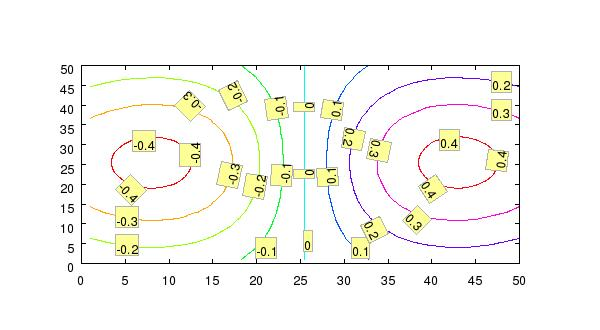
\includegraphics[width=8cm]{clabel1}}

Alternately, we can just label a subset of the contours
@>
which results in


\centerline{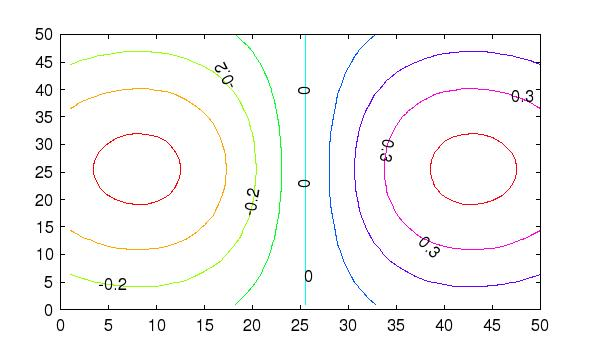
\includegraphics[width=8cm]{clabel2}}


\section{CLF Clear Figure}

\subsection{Usage}

This function clears the contents of the current figure.  The
syntax for its use is
\begin{verbatim}
   clf
\end{verbatim}

\section{CLIM Adjust Color limits of plot}

\subsection{Usage}

There are several ways to use \verb|clim| to adjust the color limits of
a plot.  The various syntaxes are
\begin{verbatim}
   clim
   clim([lo,hi])   
   clim('auto')
   clim('manual')
   clim('mode')
   clim(handle,...)
\end{verbatim}
The first form (without arguments), returns a 2-vector containing the
current limits.  The second form sets the limits on the plot to \verb|[lo,hi]|.
The third and fourth form set the mode for the limit to \verb|auto| and \verb|manual|
respectively.  In \verb|auto| mode, FreeMat chooses the range for the axis 
automatically.  The \verb|clim('mode')| form returns the current mode for the axis
(either \verb|'auto'| or \verb|'manual'|).  

Switching to \verb|manual| mode does not change the limits, it simply allows
 you to modify them (and disables the automatic adjustment of the limits
as more objects are added to the plot).  Also, if you specify a set of 
limits explicitly, the mode is set to \verb|manual|
 
Finally, you can specify the handle of an
axis to manipulate instead of using the current one.
\subsection{Example}

Here is an example of using \verb|clim| to change the effective window and
level onto an image.  First, the image with default
limits
\begin{verbatim}
--> x = repmat(linspace(-1,1),[100,1]); y = x';
--> z = exp(-x.^2-y.^2);
--> image(z);
--> min(z(:))

ans = 
    0.1353 

--> max(z(:))

ans = 
    0.9998 
\end{verbatim}
which results in


\centerline{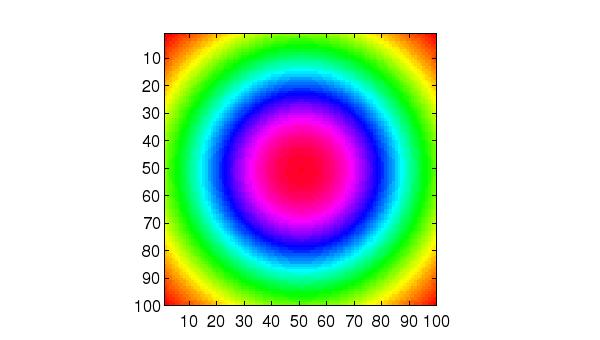
\includegraphics[width=8cm]{clim1}}

Next, we change the colorscale of the image using the
 \verb|clim| function
\begin{verbatim}
--> image(z);
--> clim([0,0.2]);
\end{verbatim}
which results in


\centerline{\includegraphics[width=8cm]{clim2}}


\section{CLOSE Close Figure Window}

\subsection{Usage}

Closes a figure window, either the currently active window, a 
window with a specific handle, or all figure windows.  The general
syntax for its use is
\begin{verbatim}
   close(handle)
\end{verbatim}
in which case the figure window with the speicified \verb|handle| is
closed.  Alternately, issuing the command with no argument
\begin{verbatim}
   close
\end{verbatim}
is equivalent to closing the currently active figure window.  Finally
the command
\begin{verbatim}
   close('all')
\end{verbatim}
closes all figure windows currently open.

\section{COLORBAR Add Colorbar to Current Plot}

\subsection{Usage}

There are a number of syntaxes for the \verb|colorbar| command.  The first
takes no arguments, and adds a vertical colorbar to the right of the current
axes.
\begin{verbatim}
  colorbar
\end{verbatim}
You can also pass properties to the newly created axes object using
the second syntax for colorbar
\begin{verbatim}
  colorbar(properties...)
\end{verbatim}

\section{COLORMAP Image Colormap Function}

\subsection{Usage}

Changes the colormap for the current figure.  The generic syntax 
for its use is
\begin{verbatim}
  colormap(map)
\end{verbatim}
where \verb|map| is a an array organized as \verb|3 \times N|),
which defines the RGB (Red Green Blue) coordinates for each color in the
colormap.  You can also use the function with no arguments to recover
the current colormap
\begin{verbatim}
  map = colormap
\end{verbatim}
\subsection{Function Internals}

Assuming that the contents of the colormap function argument \verb|c| are 
labeled as:
\[
  c = \begin{bmatrix}
    r_1 & g_1 & b_1 \\
    r_1 & g_2 & b_2 \\
    r_1 & g_3 & b_3 \\
    \vdots & \vdots & \vdots 
      \end{bmatrix} 
\]
then these columns for the RGB coordinates of pixel in the mapped image.
Assume that the image occupies the range $[a,b]$.  Then the RGB color 
of each pixel depends on the value $x$ via the following integer
\[
  k = 1 + \lfloor 256 \frac{x-a}{b-a} \rfloor,
\]
so that a pixel corresponding to image value $x$ will receive RGB color 
$[r_k,g_k,b_k]$.
Colormaps are generally used to pseudo color images to enhance 
visibility of features, etc.
\subsection{Examples}

We start by creating a smoothly varying image of a 2D Gaussian pulse.
@>
which we display with the default (grayscale) colormap here.


\centerline{\includegraphics[width=8cm]{colormap1}}


Next we switch to the \verb|copper| colormap, and redisplay the image.
@>
which results in the following image.


\centerline{\includegraphics[width=8cm]{colormap2}}


If we capture the output of the \verb|copper| command and plot it, we obtain
the following result:
@>


\centerline{\includegraphics[width=8cm]{colormap3}}


Note that in the output that each of the color components are linear functions
of the index, with the ratio between the red, blue and green components remaining
constant as a function of index.  The result is an intensity map with a copper
tint.  We can similarly construct a colormap of our own by defining the 
three components seperately.  For example, suppose we take three gaussian
curves, one for each color, centered on different parts of the index space:
@>


\centerline{\includegraphics[width=8cm]{colormap4}}


The resulting image has dark bands in it near the color transitions.
@>


\centerline{\includegraphics[width=8cm]{colormap5}}


These dark bands are a result of the nonuniform color intensity, which 
we can correct for by renormalizing each color to have the same norm.
@>


\centerline{\includegraphics[width=8cm]{colormap6}}


The resulting image has no more dark bands.
@>


\centerline{\includegraphics[width=8cm]{colormap7}}


\section{COLORSPEC Color Property Description}

\subsection{Usage}

There are a number of ways of specifying a color value for
a color-based property.  Examples include line colors, 
marker colors, and the like.  One option is to specify
color as an RGB triplet
\begin{verbatim}
   set(h,'color',[r,g,b])
\end{verbatim}
where \verb|r,g,b| are between @[0,1]@.  Alternately, you can
use color names to specify a color.
\begin{itemize}
\item  \verb|'none'| - No color.

\item  \verb|'y','yellow'| - The color @[1,1,0]@ in RGB space.

\item  \verb|'m','magenta'| - The color @[1,0,1]@ in RGB space.

\item  \verb|'c','cyan'| - The color @[0,1,1]@ in RGB space.

\item  \verb|'r','red'| - The color @[1,0,0]@ in RGB space.

\item  \verb|'g','green'| - The color @[0,1,0]@ in RGB space.

\item  \verb|'b','blue'| - The color @[0,0,1]@ in RGB space.

\item  \verb|'w','white'| - The color @[1,1,1]@ in RGB space.

\item  \verb|'k','black'| - The color @[0,0,0]@ in RGB space.

\end{itemize}

\section{CONTOUR Contour Plot Function}

\subsection{Usage}

This command generates contour plots.  There are several syntaxes for
the command.  The simplest is
\begin{verbatim}
  contour(Z)
\end{verbatim}
which generates a contour plot of the data in matrix \verb|Z|, and will
automatically select the contour levels.  The \verb|x,y| coordinates of the
contour default to \verb|1:n| and \verb|1:m|, where \verb|n| is the number of
columns and \verb|m| is the number of rows in the \verb|Z| matrix.  Alternately,
you can specify a scalar \verb|n|
\begin{verbatim}
  contour(Z,n)
\end{verbatim}
which indicates that you want \verb|n| contour levels.  For more control,
you can provide a vector \verb|v| containing the levels to contour.  If you
want to generate a contour for a particular level, you must pass a
vector \verb|[t,t]| where \verb|t| is the level you want to contour.  If you
have data that lies on a particular \verb|X,Y| grid, you can pass either
vectors \verb|x,y| or matrices \verb|X,Y| to the contour function via
\begin{verbatim}
  contour(X,Y,Z)
  contour(X,Y,Z,n)
  contour(X,Y,Z,v)
\end{verbatim}
Each form of \verb|contour| can optionally take a line spec to indicate the
color and linestyle of the contours to draw:
\begin{verbatim}
  contour(...,linespec)
\end{verbatim}
or any of the other forms of \verb|contour|.  Furthermore, you can supply an
axis to target the \verb|contour| plot to (so that it does not get added to
the current axis, which is the default):
\begin{verbatim}
  contour(axis_handle,...)
\end{verbatim}
Finally, the \verb|contour| command returns a handle to the newly returned
contour plot. 
\begin{verbatim}
  handle = contour(...)
\end{verbatim}
To place labels on the contour plot, use the \verb|clabel| function.
\subsection{Example}

Here is a simple example of a contour plot with the default \verb|x,y|
coordinates:
\begin{verbatim}
--> [x,y] = meshgrid(linspace(-1,1,25),linspace(-2,2,30));
--> z = x.*exp(-x.^2-y.^2);
--> contour(z)
\end{verbatim}
which results in the following plot


\centerline{\includegraphics[width=8cm]{contour1}}

Here, we specify the \verb|x| and \verb|y| coordinates explictly
\begin{verbatim}
--> contour(x,y,z)
\end{verbatim}
note that the axis limits have changed appropriately


\centerline{\includegraphics[width=8cm]{contour2}}

By default, contours are created at values selected by FreeMat.  To
provide our own set of contour values (asymmetrically about zero in this
case), we supply them as
\begin{verbatim}
--> contour(x,y,z,[-.4,0.,3])
\end{verbatim}
which is here


\centerline{\includegraphics[width=8cm]{contour3}}

Also be default, \verb|contour| uses the current color map and \verb|clim|
limits to determine the coloring of the contours.  Here, we override the
color spec so that we have all black contour
\begin{verbatim}
--> contour(x,y,z,'b-')
\end{verbatim}
which is here


\centerline{\includegraphics[width=8cm]{contour4}}


\section{CONTOUR3 3D Contour Plot Function}

\subsection{Usage}

This command generates contour plots where the lines are plotted in 3D.
The syntax for its use is identical to the \verb|contour| function.  Please
see its help for details.
\subsection{Example}

Here is a simple example of a 3D contour plot.
@>
The resulting plot


\centerline{\includegraphics[width=8cm]{contour3_1}}


\section{COPPER Copper Colormap}

\subsection{Usage}

Returns a copper colormap.  The syntax for its use is
\begin{verbatim}
   y = copper
\end{verbatim}
\subsection{Example}

Here is an example of an image displayed with the \verb|copper|
colormap
@>
which results in the following image


\centerline{\includegraphics[width=8cm]{copper1}}


\section{COPY Copy Figure Window}

\subsection{Usage}

Copies the currently active figure window to the clipboard.
The syntax for its use is:
\begin{verbatim}
   copy
\end{verbatim}
The resulting figure is copied as a bitmap to the clipboard, 
and can then be pasted into any suitable application.

\section{COUNTOUR Contour Object Properties}

\subsection{Usage}

Below is a summary of the properties for a line series.
\begin{itemize}
\item  \verb|contourmatrix| - \verb|array| - the matrix containing contour data
 for the plot.  This is a \verb|2 x N| matrix containing x and y coordinates
 for points on the contours.  In addition, each contour line starts with
 a column containing the number of points and the contour value.

\item  \verb|displayname| - \verb|string| - The name of this line series as it
    appears in a legend.

\item  \verb|floating| - \verb|{'on','off'}| - set to on to have floating (3D) contours

\item  \verb|levellist| - \verb|vector| - a vector of Z-values for the contours

\item  \verb|levellistmode| - \verb|{'auto','manual'}| - set to auto for 
    automatic selection  of Z-values of the contours.

\item  \verb|linecolor| - color of the contour lines.

\item  \verb|linestyle| - \verb|{'-','--',':','-.','none'}| - the line style to draw the contour in.

\item  \verb|linewidth| - \verb|scalar| - the width of the lines

\item  \verb|parent| - \verb|handle| - The axis that contains this object

\item  \verb|tag| - \verb|string| - A string that can be used to tag the object.

\item  \verb|type| - \verb|string| - Returns the string \verb|'contour'|.

\item  \verb|userdata| - \verb|array| - Available to store any variable you
 want in the handle object.

\item  \verb|visible| - \verb|{'on','off'}| - Controls visibility of the the line.

\item  \verb|xdata| - \verb|matrix| - Contains the x coordinates of the 
 surface on which the zdata is defined.  This can either be a monotonic
 vector of the same number of columns as \verb|zdata|, or a 2D matrix
 that is the same size as \verb|zdata|.

\item  \verb|xdatamode| - \verb|{'auto','manual'}| - When set to \verb|'auto'| 
FreeMat will autogenerate the x coordinates for the contours.  
These values will be \verb|1,..,N| where \verb|N| is the number of columns
of \verb|zdata|.

\item  \verb|ydata| - \verb|matrix| - Contains the y coordinates of the
 surface on which the zdata is defined.  This can either be a monotonic
 vector of the same number of rows as \verb|zdata| or a 2D matrix that is
 the same size as \verb|zdata|.

\item  \verb|ydatamode| - \verb|{'auto','manual'}| - When set to \verb|'auto'| 
FreeMat will autogenerate the y coordinates for the contour data.

\item  \verb|zdata| - \verb|matrix| - The matrix of z values that are to
 be contoured.

\end{itemize}

\section{DRAWNOW Flush the Event Queue}

\subsection{Usage}

The \verb|drawnow| function can be used to process the events in the
event queue of the FreeMat application.  The syntax for its use
is
\begin{verbatim}
   drawnow
\end{verbatim}
Now that FreeMat is threaded, you do not generally need to call this
function, but it is provided for compatibility.

\section{FIGLOWER Lower a Figure Window}

\subsection{Usage}

Lowers a figure window indicated by the figure number.  The syntax for
its use is
\begin{verbatim}
  figlower(fignum)
\end{verbatim}
where \verb|fignum| is the number of the figure to lower.  The figure will
be lowerd to the bottom of the GUI stack (meaning that it we be behind other
windows).  Note that this function does not cause \verb|fignum| to 
become the current  figure, you must use the \verb|figure| command for that.
Similarly, if \verb|fignum| is the current figure, it will remain the current
figure (even though the figure is now behind others).

\section{FIGRAISE Raise a Figure Window}

\subsection{Usage}

Raises a figure window indicated by the figure number.  The syntax for
its use is
\begin{verbatim}
  figraise(fignum)
\end{verbatim}
where \verb|fignum| is the number of the figure to raise.  The figure will
be raised to the top of the GUI stack (meaning that it we be visible).
Note that this function does not cause \verb|fignum| to become the current
figure, you must use the \verb|figure| command for that.

\section{FIGURE Figure Window Select and Create Function}

\subsection{Usage}

Changes the active figure window to the specified figure
number.  The general syntax for its use is 
\begin{verbatim}
  figure(number)
\end{verbatim}
where \verb|number| is the figure number to use. If the figure window 
corresponding to \verb|number| does not already exist, a new 
window with this number is created.  If it does exist
then it is brought to the forefront and made active.
You can use \verb|gcf| to obtain the number of the current figure.

Note that the figure number is also the handle for the figure.
While for most graphical objects (e.g., axes, lines, images), the
handles are large integers, for figures, the handle is the same
as the figure number.  This means that the figure number can be
passed to \verb|set| and \verb|get| to modify the properties of the
current figure, (e.g., the colormap).  So, for figure \verb|3|, for 
example, you can use \verb|get(3,'colormap')| to retrieve the colormap
for the current figure.

\section{FIGUREPROPERTIES Figure Object Properties}

\subsection{Usage}

Below is a summary of the properties for the axis.
\begin{itemize}
\item  \verb|alphamap| - \verb|vector| - Contains the alpha (transparency) map for the
 figure.  If this is set to a scalar, then all values are mapped to the same 
 transparency.  It defaults to \verb|1|, which is all values being fully opaque.  
 If you set this to a vector, the values of graphics objects will be mapped to 
 different transparency values, based on the setting of their \verb|alphadatamapping|
 property.

\item  \verb|color| - \verb|colorspec| - The background color of the figure (defaults to a
 gray \verb|[0.6,0.6,0.6]|).  During printing, this color is set to white, and then
 is restored.

\item  \verb|colormap| - \verb|color vector| - an \verb|N x 3| matrix of RGB values that
 specifies the colormap for the figure.  Defaults to an \verb|HSV| map.  

\item  \verb|children| - \verb|handle vector| - the handles for objects that are children
 of this figure.  These should be axis objects.

\item  \verb|currentaxes| - \verb|handle| - the handle for the current axes.  Also returned
 by \verb|gca|.

\item  \verb|doublebuffer| - Not used.

\item  \verb|parent| -  Not used.

\item  \verb|position| - Not used.

\item  \verb|type| - \verb|string| - returns the string \verb|'figure'|.

\item  \verb|userdata| - \verb|array| - arbitrary array you can use to store data associated
 with the figure.

\item  \verb|nextplot| - \verb|{'add','replace','replacechildren'}| - If set to \verb|'add'| then
 additional axes are added to the list of children for the current figure.  If set to 
 \verb|'replace'|, then a new axis replaces all of the existing children.

\item  \verb|figsize| - \verb|two vector| - the size of the figure window in pixels (width x height).

\item  \verb|renderer| - \verb|{'painters','opengl'}| - When set to \verb|'painters'| drawing is based
 on the Qt drawing methods (which can handle flat shading of surfaces with transparency).
 If you set the renderer to \verb|'opengl'| then OpenGL is used for rendering.  Support for 
 OpenGL is currently in the alpha stage, and FreeMat does not enable it automatically.
 You can set the renderer mode to \verb|'opengl'| manually to experiment.  Also, OpenGL 
 figures cannot be printed yet.

\end{itemize}

\section{GCA Get Current Axis}

\subsection{Usage}

Returns the handle for the current axis.  The syntax for its use
is
\begin{verbatim}
  handle = gca
\end{verbatim}
where \verb|handle| is the handle of the active axis.  All object
creation functions will be children of this axis.

\section{GCF Get Current Figure}

\subsection{Usage}

Returns the figure number for the current figure (which is also its handle,
and can be used to set properties of the current figure using \verb|set|).  
The syntax for its use
is
\begin{verbatim}
  figure_number = gcf
\end{verbatim}
where \verb|figure\_number| is the number of the active figure (also the handle of
the figure).

Note that figures have handles, just like axes, images, plots, etc.  However
the handles for figures match the figure number (while handles for other 
graphics objects tend to be large, somewhat arbitrary integers).  So, to 
retrieve the colormap of the current figure, you could 
use \verb|get(gcf,'colormap')|, or to obtain the colormap for figure 3, 
use \verb|get(3,'colormap')|.

\section{GET Get Object Property}

\subsection{Usage}

This function allows you to retrieve the value associated
with a property.  The syntax for its use is
\begin{verbatim}
  value = get(handle,property)
\end{verbatim}
where \verb|property| is a string containing the name of the
property, and \verb|value| is the value for that property. The
type of the variable \verb|value| depends on the property being
set.  See the help for the properties to see what values
you can set.

\section{GLSHOW Show a GL Assembly in a GL Window}

\subsection{Usage}

Shows a GL Assembly in a GL Window.  The syntax for its
use is
\begin{verbatim}
  glshow(name,scale)
\end{verbatim}
which shows the \verb|glassembly| named \verb|name| in a new GL
window, with the scale set to \verb|scale|.  Roughly speaking
\verb|scale| should represent the radial size of the object
that you want to see in the window.

\section{GRAY Gray Colormap}

\subsection{Usage}

Returns a gray colormap.  The syntax for its use is
\begin{verbatim}
   y = gray
\end{verbatim}
\subsection{Example}

Here is an example of an image displayed with the \verb|gray|
colormap
@>
which results in the following image


\centerline{\includegraphics[width=8cm]{gray1}}


\section{GRID Plot Grid Toggle Function}

\subsection{Usage}

Toggles the drawing of grid lines on the currently active plot.  The
general syntax for its use is
\begin{verbatim}
   grid(state)
\end{verbatim}
where \verb|state| is either
\begin{verbatim}
   grid('on')
\end{verbatim}
to activate the grid lines, or
\begin{verbatim}
   grid('off')
\end{verbatim}
to deactivate the grid lines.  If you specify no argument then
\verb|grid| toggles the state of the grid:
\begin{verbatim}
   grid
\end{verbatim}
You can also specify a particular axis to the grid command
\begin{verbatim}
   grid(handle,...)
\end{verbatim}
where \verb|handle| is the handle for a particular axis.
\subsection{Example}

Here is a simple plot without grid lines.
@>


\centerline{\includegraphics[width=8cm]{grid1}}


Next, we activate the grid lines.
@>


\centerline{\includegraphics[width=8cm]{grid2}}


\section{HCONTOUR Create a contour object}

\subsection{Usage}

Creates a contour object and parents it to the current axis.  The
syntax for its use is 
\begin{verbatim}
  handle = hcontour(property,value,property,value,...)
\end{verbatim}
where \verb|property| and \verb|value| are set.  The handle ID for the
resulting object is returned.  It is automatically added to
the children of the current axis.

\section{HIMAGE Create a image object}

\subsection{Usage}

Creates a image object and parents it to the current axis.  The
syntax for its use is 
\begin{verbatim}
  handle = himage(property,value,property,value,...)
\end{verbatim}
where \verb|property| and \verb|value| are set.  The handle ID for the
resulting object is returned.  It is automatically added to
the children of the current axis.

\section{HIST Histogram Function}

\subsection{Usage}

\begin{verbatim}
	n=hist (y)
	n=hist (y,x)
	n=hist (y,x,norm)
\end{verbatim}
 Produce histogram counts or plots.

 With one vector input argument, plot a histogram of the values with
 10 bins.  The range of the histogram bins is determined by the range
 of the data.

 Given a second scalar argument, use that as the number of bins.

 Given a second vector argument, use that as the centers of the bins,
 with the width of the bins determined from the adjacent values in
 the vector.

 If third argument is provided, the histogram is normalised such that
 the sum of the bars is equal to \verb|norm|.

 Extreme values are lumped in the first and last bins.


\section{HLINE Create a line object}

\subsection{Usage}

Creates a line object and parents it to the current axis.  The
syntax for its use is 
\begin{verbatim}
  handle = hline(property,value,property,value,...)
\end{verbatim}
where \verb|property| and \verb|value| are set.  The handle ID for the
resulting object is returned.  It is automatically added to
the children of the current axis.

\section{HOLD Plot Hold Toggle Function}

\subsection{Usage}

Toggles the hold state on the currently active plot.  The
general syntax for its use is
\begin{verbatim}
   hold(state)
\end{verbatim}
where \verb|state| is either
\begin{verbatim}
   hold('on')
\end{verbatim}
to turn hold on, or
\begin{verbatim}
   hold('off')
\end{verbatim}
to turn hold off. If you specify no argument then
\verb|hold| toggles the state of the hold:
\begin{verbatim}
   hold
\end{verbatim}
You can also specify a particular axis to the hold command
\begin{verbatim}
   hold(handle,...)
\end{verbatim}
where \verb|handle| is the handle for a particular axis.
\subsection{Function Internals}

The \verb|hold| function allows one to construct a plot sequence
incrementally, instead of issuing all of the plots simultaneously
using the \verb|plot| command.
\subsection{Example}

Here is an example of using both the \verb|hold| command and the
multiple-argument \verb|plot| command to construct a plot composed
of three sets of data.  The first is a plot of a modulated Gaussian.
\begin{verbatim}
--> x = linspace(-5,5,500);
--> t = exp(-x.^2);
--> y = t.*cos(2*pi*x*3);
--> plot(x,y);
\end{verbatim}


\centerline{\includegraphics[width=8cm]{hold1}}


We now turn the hold state to \verb|'on'|, and add another plot
sequence, this time composed of the top and bottom envelopes of
the modulated Gaussian.  We add the two envelopes simultaneously
using a single \verb|plot| command.  The fact that \verb|hold| is
\verb|'on'| means that these two envelopes are added to (instead of
replace) the current contents of the plot.
\begin{verbatim}
--> plot(x,y);
--> hold on
--> plot(x,t,'g-',x,-t,'b-')
\end{verbatim}


\centerline{\includegraphics[width=8cm]{hold2}}


\section{HPATCH Create a patch object}

\subsection{Usage}

Creates a patch object and parents it to the current axis.  The
syntax for its use is 
\begin{verbatim}
  handle = hpatch(property,value,property,value,...)
\end{verbatim}
where \verb|property| and \verb|value| are set.  The handle ID for the
resulting object is returned.  It is automatically added to
the children of the current axis.

\section{HPOINT Get Point From Window}

\subsection{Usage}

This function waits for the user to click on the current figure
window, and then returns the coordinates of that click.  The
generic syntax for its use is
\begin{verbatim}
  [x,y] = hpoint
\end{verbatim}

\section{HRAWPLOT Generate a Raw Plot File}

\subsection{Usage}

This function takes a sequence of commands, and generates
a raw plot (to a file) that renders the commands.  It is 
a useful tool for creating high quality fully customized 
PDF plots from within FreeMat scripts that are portable.  The
syntax for its use 
\begin{verbatim}
  hrawplot(filename,commands)
\end{verbatim}
where \verb|filename| is the name of the file to plot to, 
and \verb|commands| is a cell array of strings.  Each entry in the 
cell array contains a string with a command text.  The
commands describe a simple mini-language for describing
plots.  The complete dictionary of commands is given
\begin{itemize}
\item  \verb|LINE x1 y1 x2 y2| -- draw a line

\item  \verb|FONT name size| -- select a font of the given name and size

\item  \verb|TEXT x1 y1 string| -- draw the given text string at the given location

\item  \verb|STYLE style| -- select line style ('solid' or 'dotted')

\item  \verb|PAGE| -- force a new page

\item  \verb|SIZE x1 y1| -- Set the page mapping

\end{itemize}

\section{HSURFACE Create a surface object}

\subsection{Usage}

Creates a surface object and parents it to the current axis.  The
syntax for its use is 
\begin{verbatim}
  handle = hsurface(property,value,property,value,...)
\end{verbatim}
where \verb|property| and \verb|value| are set.  The handle ID for the
resulting object is returned.  It is automatically added to
the children of the current axis.

\section{HTEXT Create a text object}

\subsection{Usage}

Creates a text object and parents it to the current axis.  The
syntax for its use is 
\begin{verbatim}
  handle = htext(property,value,property,value,...)
\end{verbatim}
where \verb|property| and \verb|value| are set.  The handle ID for the
resulting object is returned.  It is automatically added to
the children of the current axis.

\section{HTEXTBITMAP Get Text Rendered as a Bitmap}

\subsection{Usage}

This function takes a fontname, a size, and a text string
and returns a bitmap containing the text.  The generic syntax
for its use is
\begin{verbatim}
  bitmap = htextbitmap(fontname,size,text)
\end{verbatim}
where the output bitmap contains the text rendered into a matrix.

\section{IMAGE Image Display Function}

\subsection{Usage}

The \verb|image| command has the following general syntax
\begin{verbatim}
  handle = image(x,y,C,properties...)
\end{verbatim}
where \verb|x| is a two vector containing the \verb|x| coordinates
of the first and last pixels along a column, and \verb|y| is a
two vector containing the \verb|y| coordinates of the first and
last pixels along a row.  The matrix \verb|C| constitutes the
image data.  It must either be a scalar matrix, in which case
the image is colormapped using the  \verb|colormap| for the current
figure.  If the matrix is \verb|M x N x 3|, then \verb|C| is intepreted
as RGB data, and the image is not colormapped.  The \verb|properties|
argument is a set of \verb|property/value| pairs that affect the
final image.  You can also omit the \verb|x| and \verb|y|, 
\begin{verbatim}
  handle = image(C, properties...)
\end{verbatim}
in which case they default to \verb|x = [1,size(C,2)]| and 
\verb|y = [1,size(C,1)]|.  Finally, you can use the \verb|image| function
with only formal arguments
\begin{verbatim}
  handle = image(properties...)
\end{verbatim}

To support legacy FreeMat code, you can also use the following
form of \verb|image|
\begin{verbatim}
  image(C, zoomfactor)
\end{verbatim}
which is equivalent to \verb|image(C)| with the axes removed so that
the image takes up the full figure window, and the size of the
figure window adjusted to achieve the desired zoom factor using the
\verb|zoom| command.
\subsection{Example}

In this example, we create an image that is \verb|512 x 512| pixels
square, and set the background to a noise pattern.  We set the central
\verb|128 x 256| pixels to be white.
\begin{verbatim}
--> x = rand(512);
--> x((-64:63)+256,(-128:127)+256) = 1.0;
--> figure

ans = 

 1 

--> image(x)
--> colormap(gray)
\end{verbatim}

The resulting image looks like:


\centerline{\includegraphics[width=8cm]{image1}}

Here is an example of an RGB image 
\begin{verbatim}
--> t = linspace(0,1);
--> red = t'*t;
--> green = t'*(t.^2);
--> blue = t'*(0*t+1);
--> A(:,:,1) = red; 
--> A(:,:,2) = green; 
--> A(:,:,3) = blue;
--> image(A);
\end{verbatim}
The resulting image looks like:


\centerline{\includegraphics[width=8cm]{image2}}


\section{IMAGEPROPERTIES Image Object Properties}

\subsection{Usage}

Below is a summary of the properties for the axis.
\begin{itemize}
\item  \verb|alphadata| - \verb|vector| - This is a vector that
 should contain as many elements as the image data itself \verb|cdata|,
 or a single scalar.  For a single scalar, all values of the image
 take on the same transparency.  Otherwise, the transparency of
 each pixel is determined by the corresponding value from the \verb|alphadata|
 vector.

\item  \verb|alphadatamapping| - \verb|{'scaled','direct','none'}| - For \verb|none|
 mode (the default), no transparency is applied to the data.  For \verb|direct|
 mode, the vector \verb|alphadata| contains values between @[0,M-1]| where
 \verb|M| is the length of the alpha map stored in the figure.  For \verb|scaled|
 mode, the \verb|alim| vector for the figure is used to linearly rescale the 
 alpha data prior to lookup in the alpha map. 

\item  \verb|cdata| - \verb|array| - This is either a \verb|M x N| array or an 
  \verb|M x N x 3| array.  If the data is \verb|M x N| the image is a scalar
 image (indexed mode), where the color associated with each image pixel
 is computed using the colormap and the \verb|cdatamapping| mode.  If the
 data is \verb|M x N x 3| the image is assumed to be in RGB mode, and the
 colorpanes are taken directly from \verb|cdata| (the colormap is ignored).
 Note that in this case, the data values must be between @[0,1]| for each
 color channel and each pixel.

\item  \verb|cdatamapping| - \verb|{'scaled','direct'}| - For \verb|scaled| (the
 default), the pixel values are scaled using the \verb|clim| vector for the
 figure prior to looking up in the colormap.  For \verb|direct| mode, the
 pixel values must be in the range \verb|[0,N-1| where \verb|N| is the number of
 colors in the colormap if the data is integer type.  For floating point
 data types, values must be in the range \verb|[1,N]|.

\item  \verb|children| - Not used.

\item  \verb|parent| - \verb|handle| - The axis containing the image.

\item  \verb|tag| - \verb|string| - You can set this to any string you want.

\item  \verb|type| - \verb|string| - Set to the string \verb|'image'|.

\item  \verb|xdata| - \verb|two vector| - contains the x coordinates of the
 first and last column (respectively).  Defaults to \verb|[1,C]| where
 \verb|C| is the number of columns in the image.

\item  \verb|ydata| - \verb|two vector| - contains the y coordinates of the
 first and last row (respectively).  Defaults to \verb|[1,R]| where
 \verb|R| is the number of rows in the image.

\item  \verb|userdata| - \verb|array| - Available to store any variable you
 want in the handle object.

\item  \verb|visible| - \verb|{'on','off'}| - Controls whether the image is
 visible or not.

\end{itemize}

\section{IMAGESC Image Display Function}

\subsection{Usage}

The \verb|imagesc| command has the following general syntax
\begin{verbatim}
  handle = imagesc(x,y,C,clim)
\end{verbatim}
where \verb|x| is a two vector containing the \verb|x| coordinates
of the first and last pixels along a column, and \verb|y| is a
two vector containing the \verb|y| coordinates of the first and
last pixels along a row.  The matrix \verb|C| constitutes the
image data.  It must either be a scalar matrix, in which case
the image is colormapped using the  \verb|colormap| for the current
figure.  If the matrix is \verb|M x N x 3|, then \verb|C| is intepreted
as RGB data, and the image is not colormapped.  The \verb|clim|
argument is a pairs [low high] that specifies scaling.  You can 
also omit the \verb|x| and \verb|y|, 
\begin{verbatim}
  handle = imagesc(C, clim)
\end{verbatim}
in which case they default to \verb|x = [1,size(C,2)]| and 
\verb|y = [1,size(C,1)]|.  Finally, you can use the \verb|image| function
with only formal arguments
\begin{verbatim}
  handle = imagesc(properties...)
\end{verbatim}

\subsection{Example}

In this example, we create an image that is \verb|512 x 512| pixels
square, and set the background to a noise pattern.  We set the central
\verb|128 x 256| pixels to be white.
\begin{verbatim}
--> x = rand(512);
--> x((-64:63)+256,(-128:127)+256) = 1.0;
--> figure

ans = 
 1 

--> imagesc(x,[0 .5])
--> colormap(gray)
\end{verbatim}


\section{IS2DVIEW Test Axes For 2D View}

\subsection{Usage}

This function returns \verb|true| if the current axes are in a
2-D view, and false otherwise.  The generic syntax for its
use is
\begin{verbatim}
  y = is2dview(x)
\end{verbatim}
where \verb|x| is the handle of an axes object.

\section{ISHOLD Test Hold Status}

\subsection{Usage}

Returns the state of the \verb|hold| flag on the currently active
plot.  The general syntax for its use is
\begin{verbatim}
   ishold
\end{verbatim}
and it returns a logical 1 if \verb|hold| is \verb|on|, and a logical
0 otherwise.

\section{LEGEND Add Legent to Plot}

\subsection{Usage}

This command adds a legend to the current plot.  Currently, the
following forms of the \verb|legend| command are supported.  The
first form creates a legend with the given labels for the data
series:
\begin{verbatim}
  legend('label1','label2',...)
\end{verbatim}
where \verb|'label1'| is the text label associated with data plot 1
and so on.  You can also use the \verb|legend| command to control
the appearance of the legend in the current plot.  To remove the
legend from the current plot, use
\begin{verbatim}
  legend('off')
\end{verbatim}
To hide the legend for the current plot (but do not remove it)
\begin{verbatim}
  legend('hide')
\end{verbatim}
And to show the legend that has been hidden, use
\begin{verbatim}
  legend('show')
\end{verbatim}
You can also toggle the display of the box surrounding the legend.
Use
\begin{verbatim}
  legend('boxoff')
\end{verbatim}
or 
\begin{verbatim}
  legend('boxon')
\end{verbatim}
to turn the legend box off or on, respectively.  To toggle the
visible state of the current legend, use
\begin{verbatim}
  legend('toggle')
\end{verbatim}
Specifying no arguments at all (apart from an optional location 
argument as specified below) results in the legend being rebuilt.
This form is useful for picking up font changes or relocating the
legend.
\begin{verbatim}
  legend
\end{verbatim}
By default, the \verb|legend| command places the new legend in the 
upper right corner of the current plot.  To change this behavior,
use the \verb|'location'| specifier (must be the last two options to the command)
\begin{verbatim}
  legend(...,'location',option)
\end{verbatim}
where \verb|option| takes on the following possible values
\begin{itemize}
\item  \verb|north|,\verb|N| - top center of plot 

\item  \verb|south|,\verb|S| - bottom center of plot

\item  \verb|east|,\verb|E| - middle right of plot

\item  \verb|west|,\verb|W| - middle left of plot

\item  \verb|northeast|,\verb|NE| - top right of plot (default behavior)

\item  \verb|northwest|,\verb|NW| - top left of plot

\item  \verb|southeast|,\verb|SE| - bottom right of plot

\item  \verb|southwest|,\verb|SW| - bottom left of plot

\end{itemize}
This implementation of \verb|legend| is incomplete relative to the 
MATLAB API.  The functionality will be improved in future versions
of FreeMat.

\section{LINE Line Display Function}

\subsection{Usage}

The \verb|line| command has the following general syntax
\begin{verbatim}
   handle = line(x,y,z,properties...)
\end{verbatim}
where...

\section{LINEPROPERTIES Line Series Object Properties}

\subsection{Usage}

Below is a summary of the properties for a line series.
\begin{itemize}
\item  \verb|color| - \verb|colorspec| - The color that is used to 
 draw the line.

\item  \verb|children| - Not used.

\item  \verb|displayname| - The name of this line series as it
 appears in a legend.

\item  \verb|linestyle| - \verb|{'-','--',':','-.','none'}| - The style of the line.

\item  \verb|linewidth| - \verb|scalar| - The width of the line.

\item  \verb|marker| - \verb|{'+','o','*','.','x','square','s','diamond','d','^','v','>','<'}| - 
 The marker for data points on the line.  Some of these are redundant, as \verb|'square'| 
 \verb|'s'| are synonyms, and \verb|'diamond'| and \verb|'d'| are also synonyms.

\item  \verb|markeredgecolor| - \verb|colorspec| - The color used to draw the marker.  For some
 of the markers (circle, square, etc.) there are two colors used to draw the marker.
 This property controls the edge color (which for unfilled markers) is the primary
 color of the marker.

\item  \verb|markerfacecolor| - \verb|colorspec| - The color used to fill the marker.  For some
 of the markers (circle, square, etc.) there are two colors used to fill the marker.

\item  \verb|markersize| - \verb|scalar| - Control the size of the marker.  Defaults to 6, which
 is effectively the radius (in pixels) of the markers.

\item  \verb|parent| - \verb|handle| - The axis that contains this object.

\item  \verb|tag| - \verb|string| - A string that can be used to tag the object.

\item  \verb|type| - \verb|string| - Returns the string \verb|'line'|.

\item  \verb|visible| - \verb|{'on','off'}| - Controls visibility of the the line.

\item  \verb|xdata| - \verb|vector| - Vector of x coordinates of points on the line.  Must be
 the same size as the \verb|ydata| and \verb|zdata| vectors.

\item  \verb|ydata| - \verb|vector| - Vector of y coordinates of points on the line.  Must be
 the same size as the \verb|xdata| and \verb|zdata| vectors.

\item  \verb|zdata| - \verb|vector| - Vector of z coordinates of points on the line.  Must be
 the same size as the \verb|xdata| and \verb|ydata| vectors.

\item  \verb|xdatamode| - \verb|{'auto','manual'}| - When set to \verb|'auto'| FreeMat will autogenerate
 the x coordinates for the points on the line.  These values will be \verb|1,..,N| where
 \verb|N| is the number of points in the line.

\item  \verb|userdata| - \verb|array| - Available to store any variable you
 want in the handle object.

\end{itemize}

\section{LOGLOG Log-Log Plot Function}

\subsection{Usage}

This command has the exact same syntax as the \verb|plot| command:
\begin{verbatim}
  loglog(<data 1>,{linespec 1},<data 2>,{linespec 2}...,properties...)
\end{verbatim}
in fact, it is a simple wrapper around \verb|plot| that sets the
x and y axis to have a logarithmic scale.
\subsection{Example}

Here is an example of a doubly exponential signal plotted first on a linear
plot:
@>


\centerline{\includegraphics[width=8cm]{loglog1}}

and now on a log-log plot
@>


\centerline{\includegraphics[width=8cm]{loglog2}}


\section{NEWPLOT Get Handle For Next Plot}

\subsection{Usage}

Returns the handle for the next plot operation.  The general
syntax for its use is
\begin{verbatim}
  h = newplot
\end{verbatim}
This routine checks the \verb|nextplot| properties of the current
figure and axes to see if they are set to \verb|replace| or not. If
the figures \verb|nextplot| property is set to replace, the current
figure is cleared.  If the axes \verb|nextplot| property is set to
\verb|replace| then the axes are cleared for the next operation.  

\section{PATCH Patch Graphics Function
}

\subsection{Usage}

This routine is used to create a patch object that can be plotting 2D and 3D surfaces.  A 
patch is a polygon defined by the xyz coordinates
of its vertices and optionally by the color at the vertices.
There are several forms for the \verb|patch| function:
\begin{verbatim}
  h = patch(X,Y,C,properties...)
  h = patch(X,Y,Z,C,properties...)
  h = patch(properties...)
  h = patch(V)
\end{verbatim}
Where \verb|X|, \verb|Y| and \verb|Z| are matrices or vectors of \verb|x|, \verb|y| or \verb|z| coordinates
and \verb|C| is a matrix or vector of color values (the colormap
for the current fig is applied).  
\subsection{Example}

Here we generate a surface specifying all four components.
\begin{verbatim}
--> x = [ 0 1 0 1];
--> y = [ 0 0 1 1];
--> c = [ 1 1 1 ];
--> patch(x,y,c)
--> axis equal
--> view(3)
Warning: Newly defined variable xlim shadows a function of the same name.  Use clear xlim to recover access to the function
Warning: Newly defined variable ylim shadows a function of the same name.  Use clear ylim to recover access to the function
Warning: Newly defined variable zlim shadows a function of the same name.  Use clear zlim to recover access to the function
\end{verbatim}


\centerline{\includegraphics[width=8cm]{patch1}}


\section{PCOLOR Pseudocolor Plot}

\subsection{Usage}

This routine is used to create a pseudocolor plot of the data.
A pseudocolor plot is a essentially a surface plot seen from 
above.  There are two forms for the \verb|pcolor| command:
\begin{verbatim}
   pcolor(C)
\end{verbatim}
which uses a rectangular grid.  Alternately, you can specify
\verb|X,Y| matrices or vectors.
\begin{verbatim}
   pcolor(X,Y,C)
\end{verbatim}

\section{PLOT Plot Function}

\subsection{Usage}

This is the basic plot command for FreeMat.  The general syntax for its
use is
\begin{verbatim}
  plot(<data 1>,{linespec 1},<data 2>,{linespec 2}...,properties...)
\end{verbatim}
where the \verb|<data>| arguments can have various forms, and the
\verb|linespec| arguments are optional.  We start with the
\verb|<data>| term, which can take on one of multiple forms:
\begin{itemize}
\item  Vector Matrix Case -- In this case the argument data is a pair
    of variables.  A set of \verb|x| coordinates in a numeric vector, and a 
    set of \verb|y| coordinates in the columns of the second, numeric matrix.
    \verb|x| must have as many elements as \verb|y| has columns (unless \verb|y|
    is a vector, in which case only the number of elements must match).  Each
    column of \verb|y| is plotted sequentially against the common vector \verb|x|.

\item  Unpaired Matrix Case -- In this case the argument data is a 
    single numeric matrix \verb|y| that constitutes the \verb|y|-values
    of the plot.  An \verb|x| vector is synthesized as \verb|x = 1:length(y)|,
    and each column of \verb|y| is plotted sequentially against this common \verb|x|
    axis.

\item  Complex Matrix Case -- Here the argument data is a complex
    matrix, in which case, the real part of each column is plotted against
    the imaginary part of each column.  All columns receive the same line
    styles.

\end{itemize}
Multiple data arguments in a single plot command are treated as a \emph{sequence}, meaning
that all of the plots are overlapped on the same set of axes.
The \verb|linespec| is a string used to change the characteristics of the line.  In general,
the \verb|linespec| is composed of three optional parts, the \verb|colorspec|, the 
\verb|symbolspec| and the \verb|linestylespec| in any order.  Each of these specifications
is a single character that determines the corresponding characteristic.  First, the 
\verb|colorspec|:
\begin{itemize}
\item  \verb|'b'| - Color Blue

\item  \verb|'g'| - Color Green

\item  \verb|'r'| - Color Red

\item  \verb|'c'| - Color Cyan

\item  \verb|'m'| - Color Magenta

\item  \verb|'y'| - Color Yellow

\item  \verb|'k'| - Color Black

\end{itemize}
The \verb|symbolspec| specifies the (optional) symbol to be drawn at each data point:
\begin{itemize}
\item  \verb|'.'| - Dot symbol

\item  \verb|'o'| - Circle symbol

\item  \verb|'x'| - Times symbol

\item  \verb|'+'| - Plus symbol

\item  \verb|'*'| - Asterisk symbol

\item  \verb|'s'| - Square symbol

\item  \verb|'d'| - Diamond symbol

\item  \verb|'v'| - Downward-pointing triangle symbol

\item  \verb|'\^'| - Upward-pointing triangle symbol

\item  \verb|'<'| - Left-pointing triangle symbol

\item  \verb|'>'| - Right-pointing triangle symbol

\end{itemize}
The \verb|linestylespec| specifies the (optional) line style to use for each data series:
\begin{itemize}
\item  \verb|'-'| - Solid line style

\item  \verb|':'| - Dotted line style

\item  \verb|'-.'| - Dot-Dash-Dot-Dash line style

\item  \verb|'--'| - Dashed line style

\end{itemize}
For sequences of plots, the \verb|linespec| is recycled with color order determined
by the properties of the current axes.  You can also use the \verb|properties|
argument to specify handle properties that will be inherited by all of the plots
generated during this event.  Finally, you can also specify the handle for the
axes that are the target of the \verb|plot| operation.
\begin{verbatim}
  handle = plot(handle,...)
\end{verbatim}
\subsection{Example}

The most common use of the \verb|plot| command probably involves the vector-matrix
paired case.  Here, we generate a simple cosine, and plot it using a red line, with
no symbols (i.e., a \verb|linespec| of \verb|'r-'|).
\begin{verbatim}
--> x = linspace(-pi,pi);
--> y = cos(x);
--> plot(x,y,'r-');
\end{verbatim}
which results in the following plot.


\centerline{\includegraphics[width=8cm]{plot1}}


Next, we plot multiple sinusoids (at different frequencies).  First, we construct
a matrix, in which each column corresponds to a different sinusoid, and then plot
them all at once.
\begin{verbatim}
--> x = linspace(-pi,pi);
--> y = [cos(x(:)),cos(3*x(:)),cos(5*x(:))];
--> plot(x,y);
\end{verbatim}
In this case, we do not specify a \verb|linespec|, so that we cycle through the
colors automatically (in the order listed in the previous section).


\centerline{\includegraphics[width=8cm]{plot2}}


This time, we produce the same plot, but as we want to assign individual
\verb|linespec|s to each line, we use a sequence of arguments in a single plot
command, which has the effect of plotting all of the data sets on a common 
axis, but which allows us to control the \verb|linespec| of each plot. In 
the following example, the first line (harmonic) has red, solid lines with 
times symbols
marking the data points, the second line (third harmonic) has blue, solid lines
with right-pointing triangle symbols, and the third line (fifth harmonic) has
green, dotted lines with asterisk symbols.
\begin{verbatim}
--> plot(x,y(:,1),'rx-',x,y(:,2),'b>-',x,y(:,3),'g*:');
\end{verbatim}


\centerline{\includegraphics[width=8cm]{plot3}}


The second most frequently used case is the unpaired matrix case.  Here, we need
to provide only one data component, which will be automatically plotted against
a vector of natural number of the appropriate length.  Here, we use a plot sequence
to change the style of each line to be dotted, dot-dashed, and dashed.
\begin{verbatim}
--> plot(y(:,1),'r:',y(:,2),'b;',y(:,3),'g|');
\end{verbatim}
Note in the resulting plot that the \verb|x|-axis no longer runs from \verb|[-pi,pi]|, but 
instead runs from \verb|[1,100]|.


\centerline{\includegraphics[width=8cm]{plot4}}


The final case is for complex matrices.  For complex arguments, the real part is
plotted against the imaginary part.  Hence, we can generate a 2-dimensional plot
from a vector as follows.
\begin{verbatim}
--> y = cos(2*x) + i * cos(3*x);
--> plot(y);
\end{verbatim}


\centerline{\includegraphics[width=8cm]{plot5}}


Here is an example of using the handle properties to influence the behavior
of the generated lines.
\begin{verbatim}
--> t = linspace(-3,3);
--> plot(cos(5*t).*exp(-t),'r-','linewidth',3);
\end{verbatim}


\centerline{\includegraphics[width=8cm]{plot6}}


\section{PLOT3 Plot 3D Function}

\subsection{Usage}

This is the 3D plot command.  The general syntax for its use is
\begin{verbatim}
  plot3(X,Y,Z,{linespec 1},X,Y,Z,{linespec 2},...,properties...)
\end{verbatim}
where \verb|X| \verb|Y| and \verb|Z| are the coordinates of the points on the
3D line.  Note that in general, all three should be vectors.  If
some or all of the quantities are matrices, then FreeMat will attempt
to expand the vector arguments to the same size, and then generate
multiple plots, one for each column of the matrices.  The linespec
is optional, see \verb|plot| for details.  You can specify \verb|properties|
for the generated line plots.  You can also specify a handle as an
axes to target
\begin{verbatim}
  plot3(handle,...)
\end{verbatim}
\subsection{Example}

Here is a simple example of a 3D helix.
\begin{verbatim}
--> t = linspace(0,5*pi,200);
--> x = cos(t); y = sin(t); z = t;
--> plot3(x,y,z);
Warning: Newly defined variable xlim shadows a function of the same name.  Use clear xlim to recover access to the function
Warning: Newly defined variable ylim shadows a function of the same name.  Use clear ylim to recover access to the function
Warning: Newly defined variable zlim shadows a function of the same name.  Use clear zlim to recover access to the function
--> view(3);
Warning: Newly defined variable xlim shadows a function of the same name.  Use clear xlim to recover access to the function
Warning: Newly defined variable ylim shadows a function of the same name.  Use clear ylim to recover access to the function
Warning: Newly defined variable zlim shadows a function of the same name.  Use clear zlim to recover access to the function
\end{verbatim}
Shown here


\centerline{\includegraphics[width=8cm]{plt3}}


\section{POINT Get Axis Position From Mouse Click}

\subsection{Usage}

Returns information about the currently displayed image based on a use
supplied mouse-click.  The general syntax for its use is
\begin{verbatim}
   t = point
\end{verbatim}
The returned vector \verb|y| has two elements: 
\[
  t = [x,y]
\]
where \verb|x,y| are the coordinates in the current axes of the click.  This 
function has changed since FreeMat 1.10.  If the click is not inside the
active area of any set of axes, a pair of NaNs are returned.

\section{PRINT Print a Figure To A File}

\subsection{Usage}

This function ``prints'' the currently active fig to a file.  The 
generic syntax for its use is
\begin{verbatim}
  print(filename)
\end{verbatim}
or, alternately,
\begin{verbatim}
  print filename
\end{verbatim}
where \verb|filename| is the (string) filename of the destined file.  The current
fig is then saved to the output file using a format that is determined
by the extension of the filename.  The exact output formats may vary on
different platforms, but generally speaking, the following extensions
should be supported cross-platform:
\begin{itemize}
\item  \verb|jpg|, \verb|jpeg|  --  JPEG file 

\item  \verb|pdf| -- Portable Document Format file

\item  \verb|png| -- Portable Net Graphics file

\item  \verb|svg| -- Scalable Vector Graphics file

\end{itemize}
Postscript (PS, EPS) is supported on non-Mac-OSX Unix only.
Note that only the fig is printed, not the window displaying
the fig.  If you want something like that (essentially a window-capture)
use a seperate utility or your operating system's built in screen
capture ability.
\subsection{Example}

Here is a simple example of how the figures in this manual are generated.
\begin{verbatim}
--> x = linspace(-1,1);
--> y = cos(5*pi*x);
--> plot(x,y,'r-');
--> print('printfig1.jpg')
--> print('printfig1.png')
\end{verbatim}
which creates two plots \verb|printfig1.png|, which is a Portable
Net Graphics file, and \verb|printfig1.jpg| which is a JPEG file.


\centerline{\includegraphics[width=8cm]{printfig1}}


\section{PVALID Validate Property Name}

\subsection{Usage}

This function checks to see if the given string is a valid
property name for an object of the given type.  The syntax
for its use is
\begin{verbatim}
  b = pvalid(type,propertyname)
\end{verbatim}
where \verb|string| is a string that contains the name of a 
 valid graphics object type, and
\verb|propertyname| is a string that contains the name of the
property to test for.
\subsection{Example}

Here we test for some properties on an \verb|axes| object.
\begin{verbatim}
--> pvalid('axes','type')

ans = 

 1 

--> pvalid('axes','children')

ans = 

 1 

--> pvalid('axes','foobar')

ans = 

 0 
\end{verbatim}

\section{SEMILOGX Semilog X Axis Plot Function}

\subsection{Usage}

This command has the exact same syntax as the \verb|plot| command:
\begin{verbatim}
  semilogx(<data 1>,{linespec 1},<data 2>,{linespec 2}...,properties...)
\end{verbatim}
in fact, it is a simple wrapper around \verb|plot| that sets the
x axis to have a logarithmic scale.
\subsection{Example}

Here is an example of an exponential signal plotted first on a linear
plot:
\begin{verbatim}
--> y = linspace(0,2);
--> x = (10).^y;
--> plot(x,y,'r-');
\end{verbatim}


\centerline{\includegraphics[width=8cm]{semilogx1}}

and now with a logarithmic x axis
\begin{verbatim}
--> semilogx(x,y,'r-');
\end{verbatim}


\centerline{\includegraphics[width=8cm]{semilogx2}}


\section{SEMILOGY Semilog Y Axis Plot Function}

\subsection{Usage}

This command has the exact same syntax as the \verb|plot| command:
\begin{verbatim}
  semilogy(<data 1>,{linespec 1},<data 2>,{linespec 2}...,properties...)
\end{verbatim}
in fact, it is a simple wrapper around \verb|plot| that sets the
y axis to have a logarithmic scale.
\subsection{Example}

Here is an example of an exponential signal plotted first on a linear
plot:
\begin{verbatim}
--> x = linspace(0,2);
--> y = 10.0.^x;
--> plot(x,y,'r-');
\end{verbatim}


\centerline{\includegraphics[width=8cm]{semilogy1}}

and now with a logarithmic y axis
\begin{verbatim}
--> semilogy(x,y,'r-');
\end{verbatim}


\centerline{\includegraphics[width=8cm]{semilogy2}}


\section{SET Set Object Property}

\subsection{Usage}

This function allows you to change the value associated
with a property.  The syntax for its use is
\begin{verbatim}
  set(handle,property,value,property,value,...)
\end{verbatim}
where \verb|property| is a string containing the name of the
property, and \verb|value| is the value for that property. The
type of the variable \verb|value| depends on the property being
set.  See the help for the properties to see what values
you can set.

\section{SIZEFIG Set Size of an Fig Window}

\subsection{Usage}

The \verb|sizefig| function changes the size of the currently
selected fig window.  The general syntax for its use is
\begin{verbatim}
   sizefig(width,height)
\end{verbatim}
where \verb|width| and \verb|height| are the dimensions of the fig
window.

\section{SUBPLOT Subplot Function}

\subsection{Usage}

This function divides the current figure into a 2-dimensional
grid, each of which can contain a plot of some kind.  The function
has a number of syntaxes.  The first version 
\begin{verbatim}
   subplot(row,col,num)
\end{verbatim}
which either activates subplot number \verb|num|, or 
sets up a subplot grid of size \verb|row x col|, and then
activates \verb|num|. You can also set up subplots that cover multiple
grid elements
\begin{verbatim}
   subplot(row,col,[vec])
\end{verbatim}
where \verb|vec| is a set of indexes covered by the new subplot.
Finally, as a shortcut, you can specify a string with three
components
\begin{verbatim}
   subplot('mnp')
\end{verbatim}
or using the alternate notation
\begin{verbatim}
   subplot mnp
\end{verbatim}
where \verb|m| is the number of rows, \verb|n| is the number of columns
and \verb|p| is the index.  You can also specify the location of the
subplot explicitly using the syntax
\begin{verbatim}
   subplot('position',[left bottom width height])
\end{verbatim}

\subsection{Example}

Here is the use of \verb|subplot| to set up a \verb|2 x 2| grid of plots
\begin{verbatim}
--> t = linspace(-pi,pi);
--> subplot(2,2,1)
--> plot(t,cos(t).*exp(-2*t));
--> subplot(2,2,2);
--> plot(t,cos(t*2).*exp(-2*t));
--> subplot(2,2,3);
--> plot(t,cos(t*3).*exp(-2*t));
--> subplot(2,2,4);
--> plot(t,cos(t*4).*exp(-2*t));
\end{verbatim}


\centerline{\includegraphics[width=8cm]{subplot1}}

Here we use the second form of \verb|subplot| to generate one subplot
that is twice as large.
\begin{verbatim}
--> t = linspace(-pi,pi);
--> subplot(2,2,[1,2])
--> plot(t,cos(t).*exp(-2*t));
--> subplot(2,2,3);
--> plot(t,cos(t*3).*exp(-2*t));
--> subplot(2,2,4);
--> plot(t,cos(t*4).*exp(-2*t));
\end{verbatim}


\centerline{\includegraphics[width=8cm]{subplot2}}

Note that the subplots can contain any handle graphics objects,
not only simple plots.
\begin{verbatim}
--> t=0:(2*pi/100):(2*pi);
--> x=cos(t*2).*(2+sin(t*3)*.3);
--> y=sin(t*2).*(2+sin(t*3)*.3);
--> z=cos(t*3)*.3;
--> subplot(2,2,1)
--> plot(t,x);
--> subplot(2,2,2);
--> plot(t,y);
--> subplot(2,2,3);
--> plot(t,z);
--> subplot(2,2,4);
--> tubeplot(x,y,z,0.14*sin(t*5)+.29,t,10)
--> axis equal
--> view(3)
\end{verbatim}


\centerline{\includegraphics[width=8cm]{subplot3}}


\section{SURF Surface Plot Function}

\subsection{Usage}

This routine is used to create a surface plot of data.  A 
surface plot is a 3D surface defined by the xyz coordinates
of its vertices and optionally by the color at the vertices.
The most general syntax for the \verb|surf| function is
\begin{verbatim}
  h = surf(X,Y,Z,C,properties...)
\end{verbatim}
Where \verb|X| is a matrix or vector of \verb|x| coordinates, \verb|Y| is a
matrix or vector of \verb|y| coordinates, \verb|Z| is a 2D matrix of
coordinates, and \verb|C| is a 2D matrix of color values (the colormap
for the current fig is applied).  In general, \verb|X| and \verb|Y| should
be the same size as \verb|Z|, but FreeMat will expand vectors to match
the matrix if possible.
If you want the color of the surface to be defined by the height
of the surface, you can omit \verb|C|
\begin{verbatim}
  h = surf(X,Y,Z,properties...)
\end{verbatim}
in which case \verb|C=Z|.  You can also eliminate the \verb|X| and \verb|Y|
matrices in the specification
\begin{verbatim}
  h = surf(Z,properties)
\end{verbatim}
in which case they are set to \verb|1:size(Z,2)| and \verb|1:size(Y,2)|
respectively.
You can also specify a handle as the target of the \verb|surf| command
via
\begin{verbatim}
  h = surf(handle,...)
\end{verbatim}
\subsection{Example}

Here we generate a surface specifying all four components.
\begin{verbatim}
--> x = repmat(linspace(-1,1),[100,1]);
--> y = x';
--> r = x.^2+y.^2;
--> z = exp(-r*3).*cos(5*r);
--> c = r;
--> surf(x,y,z,c)
--> axis equal
--> view(3)
Warning: Newly defined variable xlim shadows a function of the same name.  Use clear xlim to recover access to the function
Warning: Newly defined variable ylim shadows a function of the same name.  Use clear ylim to recover access to the function
Warning: Newly defined variable zlim shadows a function of the same name.  Use clear zlim to recover access to the function
\end{verbatim}


\centerline{\includegraphics[width=8cm]{surf1}}

If we allow FreeMat to specify the color component, we see that
the colorfield is the same as the height
\begin{verbatim}
--> surf(x,y,z)
--> axis equal
--> view(3)
Warning: Newly defined variable xlim shadows a function of the same name.  Use clear xlim to recover access to the function
Warning: Newly defined variable ylim shadows a function of the same name.  Use clear ylim to recover access to the function
Warning: Newly defined variable zlim shadows a function of the same name.  Use clear zlim to recover access to the function
\end{verbatim}


\centerline{\includegraphics[width=8cm]{surf2}}


\section{SURFACEPROPERTIES Surface Object Properties}

\subsection{Usage}

Below is a summary of the properties for the axis.
\begin{itemize}
\item  \verb|alphadata| - \verb|vector| - This is a vector that
 should contain as many elements as the surface data itself \verb|cdata|,
 or a single scalar.  For a single scalar, all values of the surface
 take on the same transparency.  Otherwise, the transparency of
 each pixel is determined by the corresponding value from the \verb|alphadata|
 vector.

\item  \verb|alphadatamapping| - \verb|{'scaled','direct','none'}| - For \verb|none|
 mode (the default), no transparency is applied to the data.  For \verb|direct|
 mode, the vector \verb|alphadata| contains values between @[0,M-1]| where
 \verb|M| is the length of the alpha map stored in the figure.  For \verb|scaled|
 mode, the \verb|alim| vector for the figure is used to linearly rescale the 
 alpha data prior to lookup in the alpha map. 

\item  \verb|ambientstrength| - Not used.

\item  \verb|backfacelighting| - Not used.

\item  \verb|cdata| - \verb|array| - This is either a \verb|M x N| array or an 
  \verb|M x N x 3| array.  If the data is \verb|M x N| the surface is a scalar
 surface (indexed mode), where the color associated with each surface pixel
 is computed using the colormap and the \verb|cdatamapping| mode.  If the
 data is \verb|M x N x 3| the surface is assumed to be in RGB mode, and the
 colorpanes are taken directly from \verb|cdata| (the colormap is ignored).
 Note that in this case, the data values must be between @[0,1]| for each
 color channel and each point on the surface.

\item  \verb|cdatamapping| - \verb|{'scaled','direct'}| - For \verb|scaled| (the
 default), the pixel values are scaled using the \verb|clim| vector for the
 figure prior to looking up in the colormap.  For \verb|direct| mode, the
 pixel values must be in the range \verb|[0,N-1| where \verb|N| is the number of
 colors in the colormap.

\item  \verb|children| - Not used.

\item  \verb|diffusestrength| - Not used.

\item  \verb|edgealpha| - \verb|{'flat','interp','scalar'}| - Controls how the
 transparency is mapped for the edges of the surface.

\item  \verb|edgecolor| - \verb|{'flat','interp','none',colorspec}| - Specifies
 how the edges are colored.  For \verb|'flat'| the edges are flat colored,
 meaning that the line segments that make up the edges are not shaded.
 The color for the line is determined by the first edge point it is connected
 to.

\item  \verb|edgelighting| - Not used.

\item  \verb|facealpha| - \verb|{'flat','interp','texturemap',scalar}| - Controls
 how the transparency of the faces of the surface are controlled.  For
 flat shading, the faces are constant transparency.  For interp mode, the faces
 are smoothly transparently mapped.  If set to a scalar, all faces have the
 same transparency.

\item  \verb|facecolor| - \verb|{'none','flat','interp',colorspec}| - Controls
 how the faces are colored.  For \verb|'none'| the faces are uncolored, and
 the surface appears as a mesh without hidden lines removed.  For \verb|'flat'|
 the surface faces have a constant color.  For \verb|'interp'| smooth shading
 is applied to the surface.  And if a colorspec is provided, then the
 faces all have the same color.

\item  \verb|facelighting| - Not used.

\item  \verb|linestyle| - \verb|{'-','--',':','-.','none'}| - The style of the line used
 to draw the edges.

\item  \verb|linewidth| - \verb|scalar| - The width of the line used to draw the edges.

\item  \verb|marker| - \verb|{'+','o','*','.','x','square','s','diamond','d','\^','v','>','<'}| - 
 The marker for data points on the line.  Some of these are redundant, as \verb|'square'| 
 \verb|'s'| are synonyms, and \verb|'diamond'| and \verb|'d'| are also synonyms.

\item  \verb|markeredgecolor| - \verb|colorspec| - The color used to draw the marker.  For some
 of the markers (circle, square, etc.) there are two colors used to draw the marker.
 This property controls the edge color (which for unfilled markers) is the primary
 color of the marker.

\item  \verb|markerfacecolor| - \verb|colorspec| - The color used to fill the marker.  For some
 of the markers (circle, square, etc.) there are two colors used to fill the marker.

\item  \verb|markersize| - \verb|scalar| - Control the size of the marker.  Defaults to 6, which
 is effectively the radius (in pixels) of the markers.

\item  \verb|meshstyle| - \verb|{'both','rows','cols}| - This property controls how the mesh is
 drawn for the surface.  For \verb|rows| and \verb|cols| modes, only one set of edges is drawn.

\item  \verb|normalmode| - Not used.

\item  \verb|parent| - \verb|handle| - The axis containing the surface.

\item  \verb|specularcolorreflectance| - Not used.

\item  \verb|specularexponent| - Not used.

\item  \verb|specularstrength| - Not used.

\item  \verb|tag| - \verb|string| - You can set this to any string you want.

\item  \verb|type| - \verb|string| - Set to the string \verb|'surface'|.

\item  \verb|userdata| - \verb|array| - Available to store any variable you
 want in the handle object.

\item  \verb|vertexnormals| - Not used.

\item  \verb|xdata| - \verb|array| - Must be a numeric array of size \verb|M x N| which contains
 the x location of each point in the defined surface. Must be the same size as \verb|ydata|
 and \verb|zdata|.  Alternately, you can specify an array of size \verb|1 x N| in which case
 FreeMat replicates the vector to fill out an \verb|M x N| matrix.

\item  \verb|xdatamode| - \verb|{'auto','manual'}| - When set to \verb|auto| then FreeMat will
 automatically generate the x coordinates.

\item  \verb|ydata| - \verb|array| - Must be a numeric array of size \verb|M x N| which contains
 the y location of each point in the defined surface. Must be the same size as \verb|xdata|
 and \verb|zdata|.   Alternately, you can specify an array of size \verb|M x 1| in which case
 FreeMat replicates the vector to fill out an \verb|M x N| matrix.

\item  \verb|ydatamode| - \verb|{'auto','manual'}| - When set to \verb|auto| then FreeMat will
 automatically generate the y coordinates.

\item  \verb|zdata| - \verb|array| - Must be a numeric array of size \verb|M x N| which contains
 the y location of each point in the defined surface. Must be the same size as \verb|xdata|
 and \verb|ydata|.

\item  \verb|visible| - \verb|{'on','off'}| - Controls whether the surface is
 visible or not.

\end{itemize}

\section{SURFACEPROPERTIES Surface Object Properties}

\subsection{Usage}

Below is a summary of the properties for the axis.
\begin{itemize}
\item  \verb|alphadata| - \verb|vector| - This is a vector that
 should contain as many elements as the surface data itself \verb|cdata|,
 or a single scalar.  For a single scalar, all values of the surface
 take on the same transparency.  Otherwise, the transparency of
 each pixel is determined by the corresponding value from the \verb|alphadata|
 vector.

\item  \verb|alphadatamapping| - \verb|{'scaled','direct','none'}| - For \verb|none|
 mode (the default), no transparency is applied to the data.  For \verb|direct|
 mode, the vector \verb|alphadata| contains values between @[0,M-1]| where
 \verb|M| is the length of the alpha map stored in the figure.  For \verb|scaled|
 mode, the \verb|alim| vector for the figure is used to linearly rescale the 
 alpha data prior to lookup in the alpha map. 

\item  \verb|ambientstrength| - Not used.

\item  \verb|backfacelighting| - Not used.

\item  \verb|cdata| - \verb|array| - This is either a \verb|M x N| array or an 
  \verb|M x N x 3| array.  If the data is \verb|M x N| the surface is a scalar
 surface (indexed mode), where the color associated with each surface pixel
 is computed using the colormap and the \verb|cdatamapping| mode.  If the
 data is \verb|M x N x 3| the surface is assumed to be in RGB mode, and the
 colorpanes are taken directly from \verb|cdata| (the colormap is ignored).
 Note that in this case, the data values must be between @[0,1]| for each
 color channel and each point on the surface.

\item  \verb|cdatamapping| - \verb|{'scaled','direct'}| - For \verb|scaled| (the
 default), the pixel values are scaled using the \verb|clim| vector for the
 figure prior to looking up in the colormap.  For \verb|direct| mode, the
 pixel values must be in the range \verb|[0,N-1| where \verb|N| is the number of
 colors in the colormap.

\item  \verb|children| - Not used.

\item  \verb|diffusestrength| - Not used.

\item  \verb|edgealpha| - \verb|{'flat','interp','scalar'}| - Controls how the
 transparency is mapped for the edges of the surface.

\item  \verb|edgecolor| - \verb|{'flat','interp','none',colorspec}| - Specifies
 how the edges are colored.  For \verb|'flat'| the edges are flat colored,
 meaning that the line segments that make up the edges are not shaded.
 The color for the line is determined by the first edge point it is connected
 to.

\item  \verb|edgelighting| - Not used.

\item  \verb|facealpha| - \verb|{'flat','interp','texturemap',scalar}| - Controls
 how the transparency of the faces of the surface are controlled.  For
 flat shading, the faces are constant transparency.  For interp mode, the faces
 are smoothly transparently mapped.  If set to a scalar, all faces have the
 same transparency.

\item  \verb|facecolor| - \verb|{'none','flat','interp',colorspec}| - Controls
 how the faces are colored.  For \verb|'none'| the faces are uncolored, and
 the surface appears as a mesh without hidden lines removed.  For \verb|'flat'|
 the surface faces have a constant color.  For \verb|'interp'| smooth shading
 is applied to the surface.  And if a colorspec is provided, then the
 faces all have the same color.

\item  \verb|facelighting| - Not used.

\item  \verb|linestyle| - \verb|{'-','--',':','-.','none'}| - The style of the line used
 to draw the edges.

\item  \verb|linewidth| - \verb|scalar| - The width of the line used to draw the edges.

\item  \verb|marker| - \verb|{'+','o','*','.','x','square','s','diamond','d','\^','v','>','<'}| - 
 The marker for data points on the line.  Some of these are redundant, as \verb|'square'| 
 \verb|'s'| are synonyms, and \verb|'diamond'| and \verb|'d'| are also synonyms.

\item  \verb|markeredgecolor| - \verb|colorspec| - The color used to draw the marker.  For some
 of the markers (circle, square, etc.) there are two colors used to draw the marker.
 This property controls the edge color (which for unfilled markers) is the primary
 color of the marker.

\item  \verb|markerfacecolor| - \verb|colorspec| - The color used to fill the marker.  For some
 of the markers (circle, square, etc.) there are two colors used to fill the marker.

\item  \verb|markersize| - \verb|scalar| - Control the size of the marker.  Defaults to 6, which
 is effectively the radius (in pixels) of the markers.

\item  \verb|meshstyle| - \verb|{'both','rows','cols}| - This property controls how the mesh is
 drawn for the surface.  For \verb|rows| and \verb|cols| modes, only one set of edges is drawn.

\item  \verb|normalmode| - Not used.

\item  \verb|parent| - \verb|handle| - The axis containing the surface.

\item  \verb|specularcolorreflectance| - Not used.

\item  \verb|specularexponent| - Not used.

\item  \verb|specularstrength| - Not used.

\item  \verb|tag| - \verb|string| - You can set this to any string you want.

\item  \verb|type| - \verb|string| - Set to the string \verb|'surface'|.

\item  \verb|userdata| - \verb|array| - Available to store any variable you
 want in the handle object.

\item  \verb|vertexnormals| - Not used.

\item  \verb|xdata| - \verb|array| - Must be a numeric array of size \verb|M x N| which contains
 the x location of each point in the defined surface. Must be the same size as \verb|ydata|
 and \verb|zdata|.  Alternately, you can specify an array of size \verb|1 x N| in which case
 FreeMat replicates the vector to fill out an \verb|M x N| matrix.

\item  \verb|xdatamode| - \verb|{'auto','manual'}| - When set to \verb|auto| then FreeMat will
 automatically generate the x coordinates.

\item  \verb|ydata| - \verb|array| - Must be a numeric array of size \verb|M x N| which contains
 the y location of each point in the defined surface. Must be the same size as \verb|xdata|
 and \verb|zdata|.   Alternately, you can specify an array of size \verb|M x 1| in which case
 FreeMat replicates the vector to fill out an \verb|M x N| matrix.

\item  \verb|ydatamode| - \verb|{'auto','manual'}| - When set to \verb|auto| then FreeMat will
 automatically generate the y coordinates.

\item  \verb|zdata| - \verb|array| - Must be a numeric array of size \verb|M x N| which contains
 the y location of each point in the defined surface. Must be the same size as \verb|xdata|
 and \verb|ydata|.

\item  \verb|visible| - \verb|{'on','off'}| - Controls whether the surface is
 visible or not.

\end{itemize}

\section{TEXT Add Text Label to Plot}

\subsection{Usage}

Adds a text label to the currently active plot.  The general
syntax for it is use is either
\begin{verbatim}
   text(x,y,'label')
\end{verbatim}
where \verb|x| and \verb|y| are both vectors of the same length, in which
case the text \verb|'label'| is added to the current plot at each of the
coordinates \verb|x(i),y(i)| (using the current axis to map these to screen
coordinates).  The second form supplies a cell-array of strings
as the second argument, and allows you to place many labels simultaneously
\begin{verbatim}
   text(x,y,{'label1','label2',....})
\end{verbatim}
where the number of elements in the cell array must match the size of
vectors \verb|x| and \verb|y|.  You can also specify properties for the labels
via
\begin{verbatim}
   handles = text(x,y,{labels},properties...)
\end{verbatim}
\subsection{Example}

Here is an example of a few labels being added to a random plot:
\begin{verbatim}
--> plot(rand(1,4))
--> text([2,3],[0.5,0.5],{'hello','there'})
\end{verbatim}


\centerline{\includegraphics[width=8cm]{text1}}

Here is the same example, but with larger labels:
\begin{verbatim}
--> plot(rand(1,4))
--> text([2,3],[0.5,0.5],{'hello','there'},'fontsize',20)
\end{verbatim}


\centerline{\includegraphics[width=8cm]{text2}}


\section{TEXTPROPERTIES Text Object Properties}

\subsection{Usage}

Below is a summary of the properties for a text object.
\begin{itemize}
\item  \verb|boundingbox| - \verb|four vector| - The size of the bounding
 box containing the text (in pixels).  May contain negative values
 if the text is slanted.

\item  \verb|children| - Not used.

\item  \verb|string| - \verb|string| - The text contained in the label.

\item  \verb|extent| - Not used.

\item  \verb|horizontalalignment| - \verb|{'left','center','right'}| - Controls the 
 alignment of the text relative to the specified position point.

\item  \verb|position| - \verb|three vector| - The position of the label in axis
 coordinates.

\item  \verb|rotation| - \verb|scalar| - The rotation angle (in degrees) of the label.

\item  \verb|units| - Not used.

\item  \verb|verticalalignment| - \verb|{'top','bottom','middle'}| - Controls the
 alignment fo the text relative to the specified position point in the
 vertical position.

\item  \verb|backgroundcolor| - \verb|colorspec| - The color used to fill in the background
 rectangle for the label.  Normally this is \verb|none|.

\item  \verb|edgecolor| - \verb|colorspec| - The color used to draw the bounding rectangle
 for the label.  Normally this is \verb|none|.

\item  \verb|linewidth| - \verb|scalar| - The width of the line used to draw the border.

\item  \verb|linestyle| - \verb|{'-','--',':','-.','none'}| - The style of the line used
 to draw the border.

\item  \verb|margin| - \verb|scalar| - The amount of spacing to place around the text as
 padding when drawing the rectangle.

\item  \verb|fontangle| - \verb|{'normal','italic','oblique'}| - The angle of the fonts used
 for the labels.

\item  \verb|fontsize| - \verb|scalar| - The size of fonts used for the text.

\item  \verb|fontunits| - Not used.

\item  \verb|fontweight| - \verb|{'normal','bold','light','demi'}| - The weight of the font used
 for the label

\item  \verb|visible| - \verb|{'on','off'}| - Controls visibility of the the line.

\item  \verb|color| - \verb|colorspec| - The color of the text of the label.

\item  \verb|children| - Not used.

\item  \verb|parent| - The handle of the axis that owns this label.

\item  \verb|tag| - \verb|string| - A string that can be used to tag the object.

\item  \verb|type| - \verb|string| - Returns the string \verb|'text'|.

\item  \verb|userdata| - \verb|array| - Available to store any variable you
 want in the handle object.

\end{itemize}

\section{TITLE Plot Title Function}

\subsection{Usage}

This command adds a title to the plot.  The general syntax
for its use is
\begin{verbatim}
  title('label')
\end{verbatim}
or in the alternate form
\begin{verbatim}
  title 'label'
\end{verbatim}
or simply
\begin{verbatim}
  title label
\end{verbatim}
Here \verb|label| is a string variable.  You can also specify 
properties for the label, and a handle to serve as a target
for the operation
\begin{verbatim}
  title(handle,'label',properties...)
\end{verbatim}
\subsection{Example}

Here is an example of a simple plot with a title.
\begin{verbatim}
--> x = linspace(-1,1);
--> y = cos(2*pi*x);
--> plot(x,y,'r-');
--> title('cost over time');
\end{verbatim}
which results in the following plot.


\centerline{\includegraphics[width=8cm]{title1}}

We now increase the size of the font using the properties
of the \verb|label|
\begin{verbatim}
--> title('cost over time','fontsize',20);
\end{verbatim}


\centerline{\includegraphics[width=8cm]{title2}}


\section{TUBEPLOT Creates a Tubeplot}

\subsection{Usage}

This \verb|tubeplot| function is from the tubeplot package
written by Anders Sandberg. The simplest syntax for the
\verb|tubeplot| routine is
\begin{verbatim}
    tubeplot(x,y,z)
\end{verbatim}
plots the basic tube with radius 1, where \verb|x,y,z| are
vectors that describe the tube.  If the radius of the
tube is to be varied, use the second form
\begin{verbatim}
    tubeplot(x,y,z,r) 
\end{verbatim}
which plots the basic tube with variable radius r (either 
a vector or a scalar value).  The third form allows you
to specify the coloring using a vector of values:
\begin{verbatim}
    tubeplot(x,y,z,r,v)
\end{verbatim}
where the coloring is now dependent on the values in the 
vector \verb|v|.  If you want to create a tube plot with 
a greater degree of tangential subdivisions (i.e.,
the tube is more circular, use the form
\begin{verbatim}
    tubeplot(x,y,z,r,v,s)
\end{verbatim}
where \verb|s| is the number of tangential subdivisions (default is 6)
You can also use \verb|tubeplot| to calculate matrices to feed to \verb|mesh|
and \verb|surf|.
\begin{verbatim}
    [X,Y,Z]=tubeplot(x,y,z)
\end{verbatim}
returns \verb|N x 3| matrices suitable for mesh or surf.

Note that the tube may pinch at points where the normal and binormal 
misbehaves. It is suitable for general space curves, not ones that 
contain straight sections. Normally the tube is calculated using the
Frenet frame, making the tube minimally twisted except at inflexion points.

To deal with this problem there is an alternative frame:
\begin{verbatim}
    tubeplot(x,y,z,r,v,s,vec)
\end{verbatim}
calculates the tube by setting the normal to
the cross product of the tangent and the vector vec. If it is chosen so 
that it is always far from the tangent vector the frame will not twist unduly.
\subsection{Example}

Here is an example of a \verb|tubeplot|.
\begin{verbatim}
--> t=0:(2*pi/100):(2*pi);
--> x=cos(t*2).*(2+sin(t*3)*.3);
--> y=sin(t*2).*(2+sin(t*3)*.3);
--> z=cos(t*3)*.3;
--> tubeplot(x,y,z,0.14*sin(t*5)+.29,t,10);
\end{verbatim}


\centerline{\includegraphics[width=8cm]{tubeplot1}}


 Written by Anders Sandberg, asa@nada.kth.se, 2005
 Website says the package is free for anybody to use.
 www.nada.kth.se/~asa/Ray/Tubeplot/tubeplot.html

\section{UICONTROL Create a UI Control object}

\subsection{Usage}

Creates a UI control object and parents it to the current figure.  The
syntax for its use is
\begin{verbatim}
  handle = uicontrol(property,value,property,value,...)
\end{verbatim}
where \verb|property| and \verb|value| are set.  The handle ID for the
resulting object is returned.  It is automatically added to
the children of the current figure.

\section{UICONTROLPROPERTIES UI Control Properties}

\subsection{Usage}

Below is a summary of the properties for user interface
controls.
\begin{itemize}
\item  \verb|backgroundcolor| - \verb|colorspec| - The background color
 for the widget.

\item  \verb|busyaction| - Not used.

\item  \verb|buttondownfcn| - Not used.

\item  \verb|callback| - \verb|string| - the callback to execute when the 
GUI control does its action.  Clicking a button or moving a 
scroller will cause the callback to be executed.  Also, pressing 
enter in a text box causes the callback to be executed.

\item  \verb|cdata| - an \verb|M x N x 3| array that represents an RGB image
to use as the truecolor image displayed on push bottons or toggle
buttons.  The values must be between 0 and 1.

\item  \verb|children| - Not used.

\item  \verb|createfcn| - Not used.

\item  \verb|deletefcn| - Not used;

\item  \verb|enable| - \verb|{'on','inactive','off'}| - For \verb|on| (the
default) the uicontrol behaves normally.  For inactive, it is not
operational, but looks the same as \verb|on|.  For \verb|off|, the
control is grayed out.

\item  \verb|extent| - a read only property that contains the extent of
the text for the control.

\item  \verb|fontangle| - \verb|{'normal','italic','oblique'}| - The angle of the fonts used
 for text labels (e.g., tick labels).

\item  \verb|fontsize| - \verb|scalar| - The size of fonts used for text labels (tick labels).

\item  \verb|fontunits| - Not used.

\item  \verb|fontname| - \verb|string| - The name of the font to use for the widget.

\item  \verb|fontweight| - \verb|{'normal','bold','light','demi'}| - The weight of the font used

\item  \verb|foregroundcolor| - \verb|colorspec| - the foreground color for text.

\item  \verb|handlevisibility| - Not used.

\item  \verb|hittest| - Not used.

\item  \verb|horizontalalignment| - \verb|{'left','center','right}| - determines
the justification of text.

\item  \verb|interruptible| - Not used.

\item  \verb|keypressfcn| - \verb|functionspec| - a string or function handle
 that is called when a key is pressed and a uicontrol object has focus.

\item  \verb|listboxtop| - a scalar (used only by the listbox style of
uicontrols) that specifies which string appears at the top of the list
box.

\item  \verb|max| - a scalar that specifies the largest value allowed
for the \verb|value| property.  The interpretation varies depending on
the type of the control
\begin{itemize}

\item  \verb|check boxes| - specifies what \verb|value| is set to when the
check box is selected.

\item  \verb|edit box| - if \verb|max-min>1| then the text box allows for
multiple lines of input.  Otherwise, it is a single line only.

\item  \verb|list box| - if \verb|max-min>1| then multiple item selections
are allowed.  Otherwise, only single item selections are allowed.

\item  \verb|radio buttons| - specifies what \verb|value| is set to when the
radio button is selected.

\item  \verb|slider| - the maximum value the slider can take.

\item  \verb|toggle button| - specifies what \verb|value| is set to when 
the toggle button is selected.

\end{itemize}
\item \verb|min| - a scalar that specifies the smallest value for the
\verb|value| property.  The interpretation of it depends on the type
of the control
\begin{itemize}
\item  \verb|check boxes| - specifies what \verb|value| is set to when the
check box is not selected.

\item  \verb|edit box| - if \verb|max-min>1| then the text box allows for
multiple lines of input.  Otherwise, it is a single line only.

\item  \verb|list box| - if \verb|max-min>1| then multiple item selections
are allowed.  Otherwise, only single item selections are allowed.

\item  \verb|radio buttons| - specifies what \verb|value| is set to when the
radio button is not selected.

\item  \verb|slider| - the minimum value the slider can take.

\item  \verb|toggle button| - specifies what \verb|value| is set to when 
the toggle button is not selected.

\end{itemize}
\item \verb|parent| - the handle of the parent object.
\item \verb|position| - size and location of the uicontrol as a 
four vector \verb|[left, bottom, width, height]|.  If \verb|width>height|
then sliders are horizontal, otherwise the slider is oriented
vertically.
\item \verb|selected| - \verb|{'on','off'}| - not used.
\item \verb|selectionhighlight| - \verb|{'on','off'}| - not used.
\item \verb|sliderstep| - a two vector \verb|[min_step max_step]|
that controls the amount the slider \verb|value| changes when
you click the mouse on the control.  If you click the arrow
for the slider, the value changes by \verb|min_step|, while if
you click the trough, the value changes by \verb|max_step|.  
Each value must be in the range \verb|[0,1]|, and is a percentage
of the range \verb|max-min|.
\item \verb|string| - \verb|string| - the text for the control.
\item \verb|style| - @|{'pushbutton','toggle','radiobutton','checkbox',
'edit','text','slider','frame','listbox','popupmenu'}|.
\item \verb|tag| - \verb|string| - user specified label.
\item \verb|tooltipstring| - \verb|string| the tooltip for the control.
\item \verb|type| - \verb|string| - the text is set to \verb|'uicontrol'|.
\item \verb|uicontextmenu| - \verb|handle| the handle of the \verb|uicontextmenu|
that shows up when you right-click over the control.
\item \verb|units| - not used.
\item \verb|userdata| - \verb|array| - any data you want to associate with the
control.
\item \verb|value| - The meaning of this property depends on the type of the
control:
\begin{itemize}
\item  check box - set to \verb|max| when checked, and \verb|min| when off.

\item  list box - set to a vector of indices corresponding to selected
items, with \verb|1| corresponding to the first item in the list.

\item  pop up menu - set to the index of the item selected (starting with 1)

\item  radio buttons - set to \verb|max| when selected, and set to \verb|min| when
not selected.

\item  sliders - set to the value of the slider

\item  toggle buttons - set to \verb|max| when selected, and set to \verb|min| when
not selected.

\item  text controls, push buttons - do not use this property.

\end{itemize}
\item \verb|visible| - \verb|{'on','off'}| - controls whether the control is 
visible or not
\end{itemize}

\section{VIEW Set Graphical View}

\subsection{Usage}

The \verb|view| function sets the view into the current plot.
The simplest form is
\begin{verbatim}
  view(n)
\end{verbatim}
where \verb|n=2| sets a standard view (azimuth 0 and elevation 90),
and \verb|n=3| sets a standard 3D view (azimuth 37.5 and elevation 30).
With two arguments,
\begin{verbatim}
  view(az,el)
\end{verbatim}
you set the viewpoint to azimuth \verb|az| and elevation \verb|el|.
\subsection{Example}

Here is a 3D surface plot shown with a number of viewpoints.
First, the default view for a 3D plot.
@>


\centerline{\includegraphics[width=8cm]{view1}}

Next, we look at it as a 2D plot
@>


\centerline{\includegraphics[width=8cm]{view2}}

Finally, we generate a different view of the same surface.
@>


\centerline{\includegraphics[width=8cm]{view3}}


\section{WINLEV Image Window-Level Function}

\subsection{Usage}

Adjusts the data range used to map the current image to the current
colormap.  The general syntax for its use is
\begin{verbatim}
  winlev(window,level)
\end{verbatim}
where \verb|window| is the new window, and \verb|level| is the new level, or
\begin{verbatim}
  winlev
\end{verbatim}
in which case it returns a vector containing the current window
and level for the active image.
\subsection{Function Internals}

FreeMat deals with scalar images on the range of \verb|[0,1]|, and must
therefor map an arbitrary image \verb|x| to this range before it can
be displayed.  By default, the \verb|image| command chooses 
\[
  \mathrm{window} = \max x - \min x,
\]
and
\[
  \mathrm{level} = \frac{\mathrm{window}}{2}
\]
This ensures that the entire range of image values in \verb|x| are 
mapped to the screen.  With the \verb|winlev| function, you can change
the range of values mapped.  In general, before display, a pixel \verb|x|
is mapped to \verb|[0,1]| via:
\[
   \max\left(0,\min\left(1,\frac{x - \mathrm{level}}{\mathrm{window}}
   \right)\right)
\]
\subsection{Examples}

The window level function is fairly easy to demonstrate.  Consider
the following image, which is a Gaussian pulse image that is very 
narrow:
\begin{verbatim}
--> t = linspace(-1,1,256);
--> xmat = ones(256,1)*t; ymat = xmat';
--> A = exp(-(xmat.^2 + ymat.^2)*100);
--> image(A);
\end{verbatim}
The data range of \verb|A| is \verb|[0,1]|, as we can verify numerically:
\begin{verbatim}
--> min(A(:))

ans = 

 1.3839e-87 

--> max(A(:))

ans = 

    0.9969 
\end{verbatim}
To see the tail behavior, we use the \verb|winlev| command to force FreeMat
to map a smaller range of \verb|A| to the colormap.
\begin{verbatim}
--> image(A);
--> winlev(1e-4,0.5e-4)
\end{verbatim}
The result is a look at more of the tail behavior of \verb|A|.
We can also use the winlev function to find out what the
window and level are once set, as in the following example.
\begin{verbatim}
--> image(A);
--> winlev(1e-4,0.5e-4)
--> winlev

ans = 

 1.0000e-04 
\end{verbatim}

\section{XLABEL Plot X-axis Label Function}

\subsection{Usage}

This command adds a label to the x-axis of the plot.  The general syntax
for its use is
\begin{verbatim}
  xlabel('label')
\end{verbatim}
or in the alternate form
\begin{verbatim}
  xlabel 'label'
\end{verbatim}
or simply
\begin{verbatim}
  xlabel label
\end{verbatim}
Here \verb|label| is a string variable.  You can also specify properties
for that label using the syntax
\begin{verbatim}
  xlabel('label',properties...) 
\end{verbatim}
\subsection{Example}

Here is an example of a simple plot with a label on the \verb|x|-axis.
@>
which results in the following plot.


\centerline{\includegraphics[width=8cm]{xlabel1}}


\section{XLIM Adjust X Axis limits of plot}

\subsection{Usage}

There are several ways to use \verb|xlim| to adjust the X axis limits of
a plot.  The various syntaxes are
\begin{verbatim}
   xlim
   xlim([lo,hi])   
   xlim('auto')
   xlim('manual')
   xlim('mode')
   xlim(handle,...)
\end{verbatim}
The first form (without arguments), returns a 2-vector containing the
current limits.  The second form sets the limits on the plot to \verb|[lo,hi]|.
The third and fourth form set the mode for the limit to \verb|auto| and \verb|manual|
respectively.  In \verb|auto| mode, FreeMat chooses the range for the axis 
automatically.  The \verb|xlim('mode')| form returns the current mode for the axis
(either \verb|'auto'| or \verb|'manual'|).  Finally, you can specify the handle of an
axis to manipulate instead of using the current one.
\subsection{Example}

\begin{verbatim}
--> x = linspace(-1,1);
--> y = sin(2*pi*x);
--> plot(x,y,'r-');
--> xlim  % what are the current limits?

ans = 

 -1  1 
\end{verbatim}
which results in


\centerline{\includegraphics[width=8cm]{xlim1}}

Next, we zoom in on the plot using the \verb|xlim| function
\begin{verbatim}
--> plot(x,y,'r-')
--> xlim([-0.2,0.2])
\end{verbatim}
which results in


\centerline{\includegraphics[width=8cm]{xlim2}}


\section{YLABEL Plot Y-axis Label Function}

\subsection{Usage}

This command adds a label to the y-axis of the plot.  The general syntax
for its use is
\begin{verbatim}
  ylabel('label')
\end{verbatim}
or in the alternate form
\begin{verbatim}
  ylabel 'label'
\end{verbatim}
or simply
\begin{verbatim}
  ylabel label
\end{verbatim}
You can also specify properties for that label using the syntax
\begin{verbatim}
  ylabel('label',properties...) 
\end{verbatim}
\subsection{Example}

Here is an example of a simple plot with a label on the \verb|y|-axis.
\begin{verbatim}
--> x = linspace(-1,1);
--> y = cos(2*pi*x);
--> plot(x,y,'r-');
--> ylabel('cost');
\end{verbatim}
which results in the following plot.


\centerline{\includegraphics[width=8cm]{ylabel1}}


\section{YLIM Adjust Y Axis limits of plot}

\subsection{Usage}

There are several ways to use \verb|ylim| to adjust the Y axis limits of
a plot.  The various syntaxes are
\begin{verbatim}
   ylim
   ylim([lo,hi])   
   ylim('auto')
   ylim('manual')
   ylim('mode')
   ylim(handle,...)
\end{verbatim}
The first form (without arguments), returns a 2-vector containing the
current limits.  The second form sets the limits on the plot to \verb|[lo,hi]|.
The third and fourth form set the mode for the limit to \verb|auto| and \verb|manual|
respectively.  In \verb|auto| mode, FreeMat chooses the range for the axis 
automatically.  The \verb|ylim('mode')| form returns the current mode for the axis
(either \verb|'auto'| or \verb|'manual'|).  Finally, you can specify the handle of an
axis to manipulate instead of using the current one.
\subsection{Example}

@>
which results in


\centerline{\includegraphics[width=8cm]{ylim1}}

Next, we zoom in on the plot using the \verb|ylim| function
@>
which results in


\centerline{\includegraphics[width=8cm]{ylim2}}


\section{ZLABEL Plot Z-axis Label Function}

\subsection{Usage}

This command adds a label to the z-axis of the plot.  The general syntax
for its use is
\begin{verbatim}
  zlabel('label')
\end{verbatim}
or in the alternate form
\begin{verbatim}
  zlabel 'label'
\end{verbatim}
or simply
\begin{verbatim}
  zlabel label
\end{verbatim}
Here \verb|label| is a string variable.  You can also specify properties
for that label using the syntax
\begin{verbatim}
  zlabel('label',properties...) 
\end{verbatim}
\subsection{Example}

Here is an example of a simple plot with a label on the \verb|z|-axis.
\begin{verbatim}
--> t = linspace(0,5*pi);
--> x = cos(t);
--> y = sin(t);
--> z = t;
--> plot3(x,y,z,'r-');
--> view(3);
--> zlabel('time');
\end{verbatim}
which results in the following plot.


\centerline{\includegraphics[width=8cm]{zlabel1}}


\section{ZLIM Adjust Z Axis limits of plot}

\subsection{Usage}

There are several ways to use \verb|zlim| to adjust the Z axis limits of
a plot.  The various syntaxes are
\begin{verbatim}
   zlim
   zlim([lo,hi])   
   zlim('auto')
   zlim('manual')
   zlim('mode')
   zlim(handle,...)
\end{verbatim}
The first form (without arguments), returns a 2-vector containing the
current limits.  The second form sets the limits on the plot to \verb|[lo,hi]|.
The third and fourth form set the mode for the limit to \verb|auto| and \verb|manual|
respectively.  In \verb|auto| mode, FreeMat chooses the range for the axis 
automatically.  The \verb|zlim('mode')| form returns the current mode for the axis
(either \verb|'auto'| or \verb|'manual'|).  Finally, you can specify the handle of an
axis to manipulate instead of using the current one.
\subsection{Example}

\begin{verbatim}
--> x = linspace(-1,1);
--> y = sin(2*pi*x);
--> plot(x,y,'r-');
--> zlim  % what are the current limits?

ans = 
   -0.5000    0.5000 
\end{verbatim}
which results in


\centerline{\includegraphics[width=8cm]{zlim1}}

Next, we zoom in on the plot using the \verb|zlim| function
\begin{verbatim}
--> plot(x,y,'r-')
--> zlim([-0.2,0.2])
\end{verbatim}
which results in


\centerline{\includegraphics[width=8cm]{zlim2}}


\section{ZOOM Image Zoom Function}

\subsection{Usage}

This function changes the zoom factor associated with the currently active
image.  It is a legacy support function only, and thus is not quite equivalent
to the \verb|zoom| function from previous versions of FreeMat.  However, it should
achieve roughly the same effect. The generic syntax for its use is
\begin{verbatim}
  zoom(x)
\end{verbatim}
where \verb|x| is the zoom factor to be used.  The exact behavior of the zoom
factor is as follows:
\begin{itemize}
\item  \verb|x>0| The image is zoomed by a factor \verb|x| in both directions.

\item  \verb|x=0| The image on display is zoomed to fit the size of the image window, but
  the aspect ratio of the image is not changed.  (see the Examples section for
more details).  This is the default zoom level for images displayed with the
\verb|image| command.

\item  \verb|x<0| The image on display is zoomed to fit the size of the image window, with
  the zoom factor in the row and column directions chosen to fill the entire window.
  The aspect ratio of the image is not preserved.  The exact value of \verb|x| is
  irrelevant.

\end{itemize}
\subsection{Example}

To demonstrate the use of the \verb|zoom| function, we create a rectangular image 
of a Gaussian pulse.  We start with a display of the image using the \verb|image|
command, and a zoom of 1.
\begin{verbatim}
--> x = linspace(-1,1,300)'*ones(1,600);
--> y = ones(300,1)*linspace(-1,1,600);
--> Z = exp(-(x.^2+y.^2)/0.3);
--> image(Z);
--> zoom(1.0);
\end{verbatim}


\centerline{\includegraphics[width=8cm]{zoom1}}


At this point, resizing the window accomplishes nothing, as with a zoom factor 
greater than zero, the size of the image is fixed.

If we change the zoom to another factor larger than 1, we enlarge the image by
the specified factor (or shrink it, for zoom factors \verb|0 < x < 1|.  Here is the
same image zoomed out to 60%
\begin{verbatim}
--> image(Z);
--> zoom(0.6);
\end{verbatim}


\centerline{\includegraphics[width=8cm]{zoom3}}


Similarly, we can enlarge it to 130%
\begin{verbatim}
--> image(Z)
--> zoom(1.3);
\end{verbatim}


\centerline{\includegraphics[width=8cm]{zoom4}}


The ``free'' zoom of \verb|x = 0| results in the image being zoomed to fit the window
without changing the aspect ratio.  The image is zoomed as much as possible in
one direction.
\begin{verbatim}
--> image(Z);
--> zoom(0);
--> sizefig(200,400);
\end{verbatim}


\centerline{\includegraphics[width=8cm]{zoom5}}


The case of a negative zoom \verb|x < 0| results in the image being scaled arbitrarily.
This allows the image aspect ratio to be changed, as in the following example.
\begin{verbatim}
--> image(Z);
--> zoom(-1);
--> sizefig(200,400);
\end{verbatim}


\centerline{\includegraphics[width=8cm]{zoom6}}


\section{ZPLANE Zero-pole plot}

\subsection{Usage}

 This function makes a zero-pole plot of a discrete-time
 system defined by its zeros and poles. The various syntaxes
 are
\begin{verbatim}
    zplane(z,p)
\end{verbatim}
 where \verb|z| and \verb|p| are the zeros and the poles of the system
 stored as column vectors, or
\begin{verbatim}
    zplane(b,a)
\end{verbatim}
 where \verb|a| and \verb|b| are the polynomial coefficients of the
 numerator and denominator stored as line vectors (\verb|roots| is
 used to find the zeros and poles). The symbol \verb|'o'| represents
 a zero and the symbol \verb|'x'| represents a pole. The plot includes
 the unit circle for reference.
Contributed by Paulo Xavier Candeias under GPL

\chapter{OpenGL Models}
\section{GLASSEMBLY Create a GL Assembly}

\subsection{Usage}

Define a GL Assembly.  A GL Assembly consists of one or more
GL Nodes or GL Assemblies that are placed relative to the 
coordinate system of the assembly.  For example, if we have
\verb|glnode| definitions for \verb|'bread'| and \verb|'cheese'|, then
a \verb|glassembly| of sandwich would consist of placements of
two \verb|'bread'| nodes with a \verb|'cheese'| node in between.
Furthermore, a \verb|'lunch'| assembly could consist of a \verb|'sandwich'|
a \verb|'chips'| and \verb|'soda'|.  Hopefully, you get the idea.  The
syntax for the \verb|glassembly| command is
\begin{verbatim}
   glassembly(name,part1,transform1,part2,transform2,...)
\end{verbatim}
where \verb|part1| is the name of the first part, and could be
either a \verb|glnode| or itself be another \verb|glassembly|.  
Here \verb|transform1| is the \verb|4 x 4 matrix| that transforms
the part into the local reference coordinate system.

WARNING!! Currently FreeMat does not detect or gracefully handle 
self-referential assemblies (i.e, if you try to make a \verb|sandwich| 
contain a \verb|sandwich|, which you can do by devious methods that I 
refuse to explain).  Do not do this!  You have been warned.

\section{GLCLUMP Create a GL Clump}

\subsection{Usage}

Defines an aggregate clump of objects that can be treated
as a node.  A GL Clump is defined by a vector consisting
of the following elements:
\begin{verbatim}
   [r1 g1 b1 n1 p1 p2 p3 ... r2 g2 b2 n2 p1 p2 p3 ... ]
\end{verbatim}
i.e., an RGB color spec, followed by a point count \verb|ni|, followed
by a length \verb|ni| vector of coordinates that are \verb|x,y,z| triplets.
The usage of this function is
\begin{verbatim}
   glclump(name,vector)
\end{verbatim}
where \verb|name| is the name of the clump and \verb|vector| is the aforementioned
vector of points.

\section{GLDEFMATERIAL Defines a GL Material}

\subsection{Usage}

Define a material.  The syntax for its use is
\begin{verbatim}
  gldefmaterial(name,ambient,diffuse,specular,shininess)
\end{verbatim}
where \verb|name| is the name of the material, and \verb|ambient|
is a \verb|4 x 1| vector containing the ambient component of 
the material property, and \verb|diffuse| is a \verb|4 x 1| vector
and \verb|specular| is a \verb|4 x 1| vector containing the specular
component of the material properties and \verb|shininess| is
the exponent that governs the shinines of the material.

\section{GLLINES Create a GL Lineset}

\subsection{Usage}

Defines a set of lines that can be treated as a node.
A GL Lines is defined by a vector consisting of the
following elements:
\begin{verbatim}
   [m1 x1 y1 z1 ... xn yn zn m2 x1 y1 z1 .... ]
\end{verbatim}
i.e., a point count followed by that number of triplets.
The usage of this function is 
\begin{verbatim}
  gllines(name,vector,color)
\end{verbatim}
where \verb|name| is the name of the lineset and \verb|vector|
is the aforementioned vector of points.

\section{GLNODE Create a GL Node}

\subsection{Usage}

Define a GL Node.  A GL Node is an object that can be displayed
in a GL Window.  It is defined by a triangular mesh of vertices.
It must also have a material that defines its appearance (i.e.
color, shininess, etc.).  The syntax for the \verb|glnode| command
is 
\begin{verbatim}
  glnode(name,material,pointset)  
\end{verbatim}
where \verb|material| is the name of a material that has already been
defined with \verb|gldefmaterial|, \verb|pointset| is a \verb|3 x N| matrix
of points that define the geometry of the object.  Note that the points
are assumed to be connected in triangular facts, with the points
defined counter clock-wise as seen from the outside of the facet.
\verb|FreeMat| will compute the normals.  The \verb|name| argument must
be unique.  If you want multiple instances of a given \verb|glnode|
in your GLWindow, that is fine, as instances of a \verb|glnode| are
created through a \verb|glassembly|.  

\chapter{Object Oriented Programming}
\section{AND Overloaded Logical And Operator}

\subsection{Usage}

This is a method that is invoked to combine two variables using a
logical and operator, and is invoked when you call
\begin{verbatim}
   c = and(a,b)
\end{verbatim}
or for 
\begin{verbatim}
   c = a & b
\end{verbatim}

\section{CAT Concatenation of Arrays}

\subsection{Usage}

This function concatenates arrays in a given
dimension.  The syntax for its use is
\begin{verbatim}
   cat (DIM, A, B)
   cat (DIM, A, B, C ...)
\end{verbatim}
to return the concatenation along the dimension \verb|DIM| of all arguments. 
\verb|cat(1, A, B, C)| is the same as \verb|[A; B; C]| or \verb|vertcat(A, B, C)|.
\verb|cat(2, A, B, C)| is the same as \verb|[A, B, C]| or \verb|horzcat(A, B, C)|.

\section{CLASS Class Support Function}

\subsection{Usage}

There are several uses for the \verb|class| function.  The first
version takes a single argument, and returns the class of
that variable.  The syntax for this form is
\begin{verbatim}
  classname = class(variable)
\end{verbatim}
and it returns a string containing the name of the class for
\verb|variable|.  The second form of the class function is used
to construct an object of a specific type based on a structure
which contains data elements for the class.  The syntax for
this version is
\begin{verbatim}
  classvar = class(template, classname, parent1, parent2,...)
\end{verbatim}
This should be called inside the constructor for the class.
The resulting class will be of the type \verb|classname|, and will
be derived from \verb|parent1|, \verb|parent2|, etc.  The \verb|template|
argument should be a structure array that contains the members
of the class.  See the \verb|constructors| help for some details
on how to use the \verb|class| function.  Note that if the
\verb|template| argument is an empty structure matrix, then the
resulting variable has no fields beyond those inherited from
the parent classes.

\section{COLON Overloaded Colon Operator}

\subsection{Usage}

This is a method that is invoked in one of two forms, either
the two argument version
\begin{verbatim}
  c = colon(a,b)
\end{verbatim}
which is also called using the notation
\begin{verbatim}
  c = a:b
\end{verbatim}
and the three argument version
\begin{verbatim}
  d = colon(a,b,c)
\end{verbatim}
which is also called using the notation
\begin{verbatim}
  d = a:b:c
\end{verbatim}

\section{CONSTRUCTORS Class Constructors}

\subsection{Usage}

When designing a constructor for a FreeMat class, you should
design the constructor to take a certain form.  The following
is the code for the sample \verb|mat| object 
\begin{verbatim}
function p = mat(a)
  if (nargin == 0)
    p.c = [];
    p = class(p,'mat');
  elseif isa(a,'mat')
    p = a;
  else
    p.c = a;
    p = class(p,'mat');
  end
\end{verbatim}
Generally speaking when it is provided with zero arguments, the
constructor returns a default version of the class using a template
structure with the right fields populated with default values.  If
the constructor is given a single argument that matches the class
we are trying to construct, the constructor passes through the
argument.  This form of the constructor is used for type conversion.
In particular, 
\begin{verbatim}
   p = mat(a)
\end{verbatim}
guarantees that \verb|p| is an array of class \verb|mat|.  The last form
of the constructor builds a class object given the input.  The
meaning of this form depends on what makes sense for your class.
For example, for a polynomial class, you may want to pass in the
coefficients of the polynomial.

\section{CTRANSPOSE Overloaded Conjugate Transpose Operator}

\subsection{Usage}

This is a method that is invoked when a variable has the
conjugate transpose operator method applied, and is invoked
when you call
\begin{verbatim}
   c = ctranspose(a)
\end{verbatim}
or
\begin{verbatim}
/  c = a'
\end{verbatim}

\section{EQ Overloaded Equals Comparison Operator}

\subsection{Usage}

This is a method that is invoked to combine two variables using an
equals comparison operator, and is invoked when you call
\begin{verbatim}
   c = eq(a,b)
\end{verbatim}
or for 
\begin{verbatim}
   c = a == b
\end{verbatim}

\section{GE Overloaded Greater-Than-Equals Comparison Operator}

\subsection{Usage}

This is a method that is invoked to combine two variables using a
greater than or equals comparison operator, and is invoked when you call
\begin{verbatim}
   c = ge(a,b)
\end{verbatim}
or for 
\begin{verbatim}
   c = a >= b
\end{verbatim}

\section{GT Overloaded Greater Than Comparison Operator}

\subsection{Usage}

This is a method that is invoked to combine two variables using a
greater than comparison operator, and is invoked when you call
\begin{verbatim}
   c = gt(a,b)
\end{verbatim}
or for 
\begin{verbatim}
   c = a > b
\end{verbatim}

\section{HORZCAT Horizontal Array Concatenation}

\subsection{Usage}

This function concatenates arrays horizontally (along the column
dimension).  The syntax for its use is
\begin{verbatim}
   d = horzcat(a,b,c)
\end{verbatim}
which is equivalent to the statement \verb|d = [a,b,c]|.

\section{HORZCAT Horizontal Array Concatenation}

\subsection{Usage}

This function concatenates arrays horizontally (along the column
dimension).  The syntax for its use is
\begin{verbatim}
   d = horzcat(a,b,c)
\end{verbatim}
which is equivalent to the statement \verb|d = [a,b,c]|.

\section{LDIVIDE Overloaded Left Divide Operator}

\subsection{Usage}

This is a method that is invoked when two variables are divided
and is invoked when you call
\begin{verbatim}
   c = ldivide(a,b)
\end{verbatim}
or for
\begin{verbatim}
   c = a .\ b
\end{verbatim}

\section{LE Overloaded Less-Than-Equals Comparison Operator}

\subsection{Usage}

This is a method that is invoked to compare two variables using a
less than or equals comparison operator, and is invoked when you call
\begin{verbatim}
   c = le(a,b)
\end{verbatim}
or for 
\begin{verbatim}
   c = a <= b
\end{verbatim}

\section{LT Overloaded Less Than Comparison Operator}

\subsection{Usage}

This is a method that is invoked to compare two variables using a
less than comparison operator, and is invoked when you call
\begin{verbatim}
   c = lt(a,b)
\end{verbatim}
or for 
\begin{verbatim}
   c = a < b
\end{verbatim}

\section{MINUS Overloaded Addition Operator}

\subsection{Usage}

This is a method that is invoked when two variables are subtracted
and is invoked when you call
\begin{verbatim}
   c = minus(a,b)
\end{verbatim}
or for
\begin{verbatim}
   c = a - b
\end{verbatim}

\section{MLDIVIDE Overloaded Matrix Left Divide Operator}

\subsection{Usage}

This is a method that is invoked when two variables are divided
using the matrix (left) divide operator, and is invoked when
you call
\begin{verbatim}
   c = mldivide(a,b)
\end{verbatim}
or for
\begin{verbatim}
   c = a \ b
\end{verbatim}

\section{MPOWER Overloaded Matrix Power Operator}

\subsection{Usage}

This is a method that is invoked when one variable is raised
to another variable using the matrix power operator, and
is invoked when you call
\begin{verbatim}
  c = mpower(a,b)
\end{verbatim}
or
\begin{verbatim}
  c = a^b
\end{verbatim}

\section{MRDIVIDE Overloaded Matrix Right Divide Operator}

\subsection{Usage}

This is a method that is invoked when two variables are divided
using the matrix divide operator, and is invoked when you call
\begin{verbatim}
   c = mrdivide(a,b)
\end{verbatim}
or for
\begin{verbatim}
   c = a / b
\end{verbatim}

\section{MTIMES Overloaded Matrix Multiplication Operator}

\subsection{Usage}

This is a method that is invoked when two variables are multiplied
using the matrix operator and is invoked when you call
\begin{verbatim}
   c = mtimes(a,b)
\end{verbatim}
or for
\begin{verbatim}
   c = a * b
\end{verbatim}

\section{NE Overloaded Not-Equals Comparison Operator}

\subsection{Usage}

This is a method that is invoked to combine two variables using a
not-equals comparison operator, and is invoked when you call
\begin{verbatim}
   c = ne(a,b)
\end{verbatim}
or for 
\begin{verbatim}
   c = a != b
\end{verbatim}

\section{NOT Overloaded Logical Not Operator}

\subsection{Usage}

This is a method that is invoked when a variable is logically
inverted, and is invoked when you call
\begin{verbatim}
   c = not(a)
\end{verbatim}
or for
\begin{verbatim}
   c = ~a
\end{verbatim}

\section{OR Overloaded Logical Or Operator}

\subsection{Usage}

This is a method that is invoked to combine two variables using a
logical or operator, and is invoked when you call
\begin{verbatim}
   c = or(a,b)
\end{verbatim}
or for 
\begin{verbatim}
   c = a | b
\end{verbatim}

\section{PLUS Overloaded Addition Operator}

\subsection{Usage}

This is a method that is invoked when two variables are added
and is invoked when you call
\begin{verbatim}
   c = plus(a,b)
\end{verbatim}
or for
\begin{verbatim}
   c = a + b
\end{verbatim}

\section{POWER Overloaded Power Operator}

\subsection{Usage}

This is a method that is invoked when one variable is raised
to another variable using the dot-power operator, and is
invoked when you call
\begin{verbatim}
   c = power(a,b)
\end{verbatim}
or
\begin{verbatim}
   c = a.^b
\end{verbatim}

\section{RDIVIDE Overloaded Right Divide Operator}

\subsection{Usage}

This is a method that is invoked when two variables are divided
and is invoked when you call
\begin{verbatim}
   c = rdivide(a,b)
\end{verbatim}
or for
\begin{verbatim}
   c = a ./ b
\end{verbatim}

\section{SUBSASGN Overloaded Class Assignment}

\subsection{Usage}

This method is called for expressions of the form
\begin{verbatim}
  a(b) = c, a{b} = c, a.b = c
\end{verbatim}
and overloading the \verb|subsasgn| method can allow you
to define the meaning of these expressions for
objects of class \verb|a|.  These expressions are mapped
to a call of the form
\begin{verbatim}
  a = subsasgn(a,s,b)
\end{verbatim}
where \verb|s| is a structure array with two fields.  The
first field is
\begin{itemize}
\item  \verb|type|  is a string containing either \verb|'()'| or
 \verb|'{}'| or \verb|'.'| depending on the form of the call.

\item  \verb|subs| is a cell array or string containing the
 the subscript information.

\end{itemize}
When multiple indexing experssions are combined together
such as \verb|a(5).foo{:} = b|, the \verb|s| array contains
the following entries
\begin{verbatim}
  s(1).type = '()'  s(1).subs = {5}
  s(2).type = '.'   s(2).subs = 'foo'
  s(3).type = '{}'  s(3).subs = ':'
\end{verbatim}

\section{SUBSINDEX Overloaded Class Indexing}

\subsection{Usage}

This method is called for classes in the expressions
of the form
\begin{verbatim}
  c = subsindex(a)
\end{verbatim}
where \verb|a| is an object, and \verb|c| is an index vector.
It is also called for
\begin{verbatim}
  c = b(a)
\end{verbatim}
in which case \verb|subsindex(a)| must return a vector containing
integers between \verb|0| and \verb|N-1| where \verb|N| is the number
of elements in the vector \verb|b|.

\section{SUBSREF Overloaded Class Indexing}

\subsection{Usage}

This method is called for expressions of the form
\begin{verbatim}
  c = a(b), c = a{b}, c = a.b
\end{verbatim}
and overloading the \verb|subsref| method allows you
to define the meaning of these expressions for
objects of class \verb|a|.  These expressions are
mapped to a call of the form
\begin{verbatim}
  b = subsref(a,s)
\end{verbatim}
where \verb|s| is a structure array with two fields. The
first field is
\begin{itemize}
\item  \verb|type|  is a string containing either \verb|'()'| or
 \verb|'{}'| or \verb|'.'| depending on the form of the call.

\item  \verb|subs| is a cell array or string containing the
 the subscript information.

\end{itemize}
When multiple indexing experssions are combined together
such as \verb|b = a(5).foo{:}|, the \verb|s| array contains
the following entries
\begin{verbatim}
  s(1).type = '()'  s(1).subs = {5}
  s(2).type = '.'   s(2).subs = 'foo'
  s(3).type = '{}'  s(3).subs = ':'
\end{verbatim}

\section{TIMES Overloaded Multiplication Operator}

\subsection{Usage}

This is a method that is invoked when two variables are multiplied
and is invoked when you call
\begin{verbatim}
   c = times(a,b)
\end{verbatim}
or for
\begin{verbatim}
   c = a .* b
\end{verbatim}

\section{TRANSPOSE Overloaded Transpose Operator}

\subsection{Usage}

This is a method that is invoked when a variable has the
transpose operator method applied, and is invoked
when you call
\begin{verbatim}
   c = transpose(a)
\end{verbatim}
or
\begin{verbatim}
/  c = a.'
\end{verbatim}

\section{UMINUS Overloaded Unary Minus Operator}

\subsection{Usage}

This is a method that is invoked when a variable is negated,
and is invoked when you call
\begin{verbatim}
   c = uminus(a)
\end{verbatim}
or for 
\begin{verbatim}
   c = -a
\end{verbatim}

\section{UPLUS Overloaded Unary Plus Operator}

\subsection{Usage}

This is a method that is invoked when a variable is preceeded by a "+",
and is invoked when you call
\begin{verbatim}
   c = uplus(a)
\end{verbatim}
or for 
\begin{verbatim}
   c = +a
\end{verbatim}

\section{VERTCAT Overloaded Vertical Concatenation}

\subsection{Usage}

This is a method for a class that is invoked to concatenate two or more
variables of the same class type together.  Besides being called when
you invoke
\begin{verbatim}
   c = vertcat(a,b,c)
\end{verbatim}
when \verb|a| is a class, it is also called for
\begin{verbatim}
   c = [a;b;c]
\end{verbatim}
when one of the variables is a class.  The exact meaning of 
vertical concatenation depends on the class you have designed.

\section{VERTCAT Overloaded Vertical Concatenation}

\subsection{Usage}

This is a method for a class that is invoked to concatenate two or more
variables of the same class type together.  Besides being called when
you invoke
\begin{verbatim}
   c = vertcat(a,b,c)
\end{verbatim}
when \verb|a| is a class, it is also called for
\begin{verbatim}
   c = [a;b;c]
\end{verbatim}
when one of the variables is a class.  The exact meaning of 
vertical concatenation depends on the class you have designed.

\chapter{Bitwise Operations}
\section{BITAND Bitwise Boolean And Operation}

\subsection{Usage}

Performs a bitwise binary and operation on the two arguments and
returns the result.  The syntax for its use is
\begin{verbatim}
   y = bitand(a,b)
\end{verbatim}
where \verb|a| and \verb|b| are multi-dimensional unsigned integer arrays.
The and operation is performed using 32 bit unsigned intermediates.  Note that if a
or b is a scalar, then each element of the other array is and'ed with
 that scalar.  Otherwise the two arrays must match in size.
\subsection{Example}

@>

\section{BITCMP Bitwise Boolean Complement Operation}

\subsection{Usage}

 Usage
 
 Performs a bitwise binary complement operation on the argument and
 returns the result.  The syntax for its use is
\begin{verbatim}
    y = bitcmp(a)
\end{verbatim}
 where a is an unsigned integer arrays.  This version of the command
 uses as many bits as required by the type of a.  For example, if 
 a is an uint8 type, then the complement is formed using 8 bits.
 The second form of bitcmp allows you to specify the number of bits
 to use, 
\begin{verbatim}
    y = bitcmp(a,n)
\end{verbatim}
 in which case the complement is taken with respect to n bits, where n must be 
 less than the length of the integer type.

\subsection{Example}

\begin{verbatim}
--> bitcmp(uint16(2^14-2))

ans = 

 65535 

--> bitcmp(uint16(2^14-2),14)

ans = 

 16383 
\end{verbatim}

\section{BITOR Bitwise Boolean Or Operation}

\subsection{Usage}

Performs a bitwise binary or operation on the two arguments and
returns the result.  The syntax for its use is
\begin{verbatim}
   y = bitor(a,b)
\end{verbatim}
where \verb|a| and \verb|b| are multi-dimensional unsigned integer arrays.
The and operation is performed using 32 bit unsigned intermediates.  Note that if a
or b is a scalar, then each element of the other array is or'ed with
that scalar.  Otherwise the two arrays must match in size.
\subsection{Example}

\begin{verbatim}
--> bitand(uint16([1,16,255]),uint16([3,17,128]))

ans = 

   1  16 128 

--> bitand(uint16([1,16,255]),uint16(3))

ans = 

 1 0 3 
\end{verbatim}

\section{BITXOR Bitwise Boolean Exclusive-Or (XOR) Operation}

\subsection{Usage}

Performs a bitwise binary xor operation on the two arguments and
returns the result.  The syntax for its use is
\begin{verbatim}
   y = bitxor(a,b)
\end{verbatim}
where \verb|a| and \verb|b| are multi-dimensional unsigned integer arrays.
The and operation is performed using 32 bit unsigned intermediates.  Note that if a
or b is a scalar, then each element of the other array is xor'ed with
 that scalar.  Otherwise the two arrays must match in size.
\subsection{Example}

\begin{verbatim}
--> bitand(uint16([1,16,255]),uint16([3,17,128]))

ans = 
   1  16 128 

--> bitand(uint16([1,16,255]),uint16(3))

ans = 
 1 0 3 
\end{verbatim}

\chapter{FreeMat Threads}
\section{THREADCALL Call Function In A Thread}

\subsection{Usage}

The \verb|threadcall| function is a convenience function for executing
a function call in a thread.  The syntax for its use is
\begin{verbatim}
   [val1,...,valn] = threadcall(threadid,timeout,funcname,arg1,arg2,...)
\end{verbatim}
where \verb|threadid| is the ID of the thread (as returned by the
\verb|threadnew| function), \verb|funcname| is the name of the function to call,
and \verb|argi| are the arguments to the function, and \verb|timeout| is the
amount of time (in milliseconds) that the function is allowed to take.
\subsection{Example}

Here is an example of executing a simple function in a different thread.
\begin{verbatim}
--> id = threadnew

id = 
 3 

--> d = threadcall(id,1000,'cos',1.02343)

d = 
    0.5204 

--> threadfree(id)
\end{verbatim}

\section{THREADFREE Free thread resources}

\subsection{Usage}

The \verb|threadfree| is a function to free the resources claimed
by a thread that has finished.  The syntax for its use is
\begin{verbatim}
   threadfree(handle)
\end{verbatim}
where \verb|handle| is the handle returned by the call to \verb|threadnew|.
The \verb|threadfree| function requires that the thread be completed.  
Otherwise it will wait for the thread to complete, potentially 
for an arbitrarily long period of time.  To fix this, you can
either call \verb|threadfree| only on threads that are known to have
completed, or you can call it using the syntax
\begin{verbatim}
   threadfree(handle,timeout)
\end{verbatim}
where \verb|timeout| is a time to wait in milliseconds.  If the thread
fails to complete before the timeout expires, an error occurs.

\section{THREADID Get Current Thread Handle}

\subsection{Usage}

The \verb|threadid| function in FreeMat tells you which thread
is executing the context you are in.  Normally, this is thread
1, the main thread.  However, if you start a new thread using
\verb|threadnew|, you will be operating in a new thread, and functions
that call \verb|threadid| from the new thread will return their 
handles.
\subsection{Example}

From the main thread, we have
\begin{verbatim}
--> threadid

ans = 
 2 
\end{verbatim}
But from a launched auxilliary thread, we have
\begin{verbatim}
--> t_id = threadnew

t_id = 
 3 

--> id = threadcall(t_id,1000,'threadid')

id = 
 3 

--> threadfree(t_id);
\end{verbatim}

\section{THREADKILL Halt execution of a thread}

\subsection{Usage}

The \verb|threadkill| function stops (or attempts to stop) execution
of the given thread.  It works only for functions defined in M-files
(i.e., not for built in or imported functions), and it works by 
setting a flag that causes the thread to stop execution at the next
available statement.  The syntax for this function is 
\begin{verbatim}
  threadkill(handle)
\end{verbatim}
where \verb|handle| is the value returned by a \verb|threadnew| call.  
Note that the \verb|threadkill| function returns immediately.  It 
is still your responsibility to call \verb|threadfree| to free
the thread you have halted.

You cannot kill the main thread (thread id \verb|1|).
\subsection{Example}

Here is an example of stopping a runaway thread using \verb|threadkill|.
Note that the thread function in this case is an M-file function.
We start by setting up a free running counter, where we can access 
the counter from the global variables.  
\begin{verbatim}
    freecount.m
function freecount
  global count
  if (~exist('count')) count = 0; end  % Initialize the counter
  while (1)
    count = count + 1;                 % Update the counter
  end
\end{verbatim}
We now launch this function in a thread, and use \verb|threadkill| to
stop it:
\begin{verbatim}
--> a = threadnew;
--> global count                   % register the global variable count
--> count = 0;
--> threadstart(a,'freecount',0)   % start the thread
--> count                          % it is counting

ans = 
 70 

--> sleep(1)                       % Wait a bit
--> count                          % it is still counting

ans = 
 545650 

--> threadkill(a)                  % kill the counter
--> threadwait(a,1000)             % wait for it to finish

ans = 
 1 

--> count                          % The count will no longer increase

ans = 
 545729 

--> sleep(1)
--> count

ans = 
 545729 

--> threadfree(a)
\end{verbatim}

\section{THREADNEW Create a New Thread}

\subsection{Usage}

The \verb|threadnew| function creates a new FreeMat thread, and
returns a handle to the resulting thread.   The \verb|threadnew|
function takes no arguments.  They general syntax for the
\verb|threadnew| function is
\begin{verbatim}
   handle = threadnew
\end{verbatim}
Once you have a handle to a thread, you can start the thread
on a computation using the \verb|threadstart| function.  The
threads returned by \verb|threadnew| are in a dormant state (i.e.,
not running).  Once you are finished with the thread you
must call \verb|threadfree| to free the resources associated with
that thread.

Some additional important information.  Thread functions operate
in their own context or workspace, which means that data cannot
be shared between threads.  The exception is \verb|global| variables,
which provide a thread-safe way for multiple threads to share data.
Accesses to global variables are serialized so that they can 
be used to share data.  Threads and FreeMat are a new feature, so
there is room for improvement in the API and behavior.  The best
way to improve threads is to experiment with them, and send feedback.

\section{THREADSTART Start a New Thread Computation}

\subsection{Usage}

The \verb|threadstart| function starts a new computation on a
FreeMat thread, and you must provide a function (no scripts 
are allowed) to run inside the thread, pass any parameters that
the thread function requires, as well as the number of output
arguments expected.  The general syntax for the 
\verb|threadstart| function is
\begin{verbatim}
   threadstart(threadid,function,nargout,arg1,arg2,...)
\end{verbatim}
where \verb|threadid| is a thread handle (returned by \verb|threadnew|),
where \verb|function| is a valid function name (it can be a built-in
imported or M-function), \verb|nargout| is the number of output arguments
expected from the function, and \verb|arg1| is the first argument that
is passed to the function.  Because the function runs in its 
own thread, the return values of the function are not available
imediately.  Instead, execution of that function will continue
in parallel with the current thread.  To retrieve the output
of the thread function, you must wait for the thread to complete
using the \verb|threadwait| function, and then call \verb|threadvalue|
 to retrieve the result.  You can also stop the running thread
prematurely by using the \verb|threadkill| function.  It is important
to call \verb|threadfree| on the handle you get from \verb|threadnew|
when you are finished with the thread to ensure that the resoures
are properly freed.  

It is also perfectly reasonable to use a single thread multiple
times, calling \verb|threadstart| and \verb|threadreturn| multiple times
on a single thread.  The context is preserved between threads.
When calling \verb|threadstart| on a pre-existing thread, FreeMat
will attempt to wait on the thread.  If the wait fails, then
an error will occur.

Some additional important information.  Thread functions operate
in their own context or workspace, which means that data cannot
be shared between threads.  The exception is \verb|global| variables,
which provide a thread-safe way for multiple threads to share data.
Accesses to global variables are serialized so that they can 
be used to share data.  Threads and FreeMat are a new feature, so
there is room for improvement in the API and behavior.  The best
way to improve threads is to experiment with them, and send feedback.

\subsection{Example}

Here we do something very simple.  We want to obtain a listing of
all files on the system, but do not want the results to stop our
computation.  So we run the \verb|system| call in a thread.
\begin{verbatim}
--> a = threadnew;                         % Create the thread
--> threadstart(a,'system',1,'ls -lrt /'); % Start the thread
--> b = rand(100)\rand(100,1);             % Solve some equations simultaneously
--> c = threadvalue(a);                    % Retrieve the file list
--> size(c)                                % It is large!

ans = 
  1 27 

--> threadfree(a);
\end{verbatim}
The possibilities for threads are significant.  For example,
we can solve equations in parallel, or take Fast Fourier Transforms
on multiple threads.  On multi-processor machines or multicore CPUs,
these threaded calculations will execute in parallel.  Neat.

The reason for the  \verb|nargout| argument is best illustrated with
an example.  Suppose we want to compute the Singular Value 
Decomposition \verb|svd| of a matrix \verb|A| in a thread.  
The documentation for the \verb|svd| function tells us that
the behavior depends on the number of output arguments we request.
For example, if we want a full decomposition, including the left 
and right singular vectors, and a diagonal singular matrix, we
need to use the three-output syntax, instead of the single output
syntax (which returns only the singular values in a column vector):
\begin{verbatim}
--> A = float(rand(4))

A = 
    0.4011    0.4747    0.9193    0.8655 
    0.8633    0.0123    0.0599    0.5917 
    0.4939    0.5458    0.9481    0.4566 
    0.9335    0.8614    0.7993    0.6394 

--> [u,s,v] = svd(A)    % Compute the full decomposition
u = 
   -0.5290    0.2711    0.7178    0.3626 
   -0.3004   -0.8911    0.2379   -0.2431 
   -0.4868    0.3556   -0.0927   -0.7925 
   -0.6269   -0.0778   -0.6478    0.4259 

s = 
    2.5579         0         0         0 
         0    0.7905         0         0 
         0         0    0.4392         0 
         0         0         0    0.1705 

v = 
   -0.5071   -0.7054   -0.3579   -0.3422 
   -0.4146    0.3096   -0.6032    0.6070 
   -0.5735    0.5955    0.1558   -0.5406 
   -0.4921   -0.2279    0.6955    0.4713 

--> sigmas = svd(A)     % Only want the singular values

sigmas = 
    2.5579 
    0.7905 
    0.4392 
    0.1705 
\end{verbatim}

Normally, FreeMat uses the left hand side of an assignment to calculate
the number of outputs for the function.  When running a function in a
thread, we separate the assignment of the output from the invokation
of the function.  Hence, we have to provide the number of arguments at the
time we invoke the function.  For example, to compute a full decomposition
in a thread, we specify that we want 3 output arguments:
\begin{verbatim}
--> a = threadnew;               % Create the thread
--> threadstart(a,'svd',3,A);    % Start a full decomposition 
--> [u1,s1,v1] = threadvalue(a); % Retrieve the function values
--> threadfree(a);
\end{verbatim}
If we want to compute just the singular values, we start the thread
function with only one output argument:
\begin{verbatim}
--> a = threadnew;
--> threadstart(a,'svd',1,A);
--> sigmas = threadvalue(a);
--> threadfree(a)
\end{verbatim}

\section{THREADVALUE Retrieve the return values from a thread}

\subsection{Usage}

The \verb|threadvalue| function retrieves the values returned
by the function specified in the \verb|threadnew| call.  The
syntax for its use is
\begin{verbatim}
   [arg1,arg2,...,argN] = threadvalue(handle)
\end{verbatim}
where \verb|handle| is the value returned by a \verb|threadnew| call.
Note that there are issues with \verb|nargout|.  See the examples
section of \verb|threadnew| for details on how to work around this
limitation.  Because the function you have spawned with \verb|threadnew|
may still be executing, \verb|threadvalue| must first \verb|threadwait|
for the function to complete before retrieving the output values.
This wait may take an arbitrarily long time if the thread function
is caught in an infinite loop.  Hence, you can also specify
a timeout parameter to \verb|threadvalue| as
\begin{verbatim}
   [arg1,arg2,...,argN] = threadvalue(handle,timeout)
\end{verbatim}
where the \verb|timeout| is specified in milliseconds.  If the
wait times out, an error is raised (that can be caught with a
\verb|try| and \verb|catch| block.  

In either case, if the thread function itself caused an error
and ceased execution abruptly, then calling \verb|threadvalue| will
cause that function to raise an error, allowing you to retrieve
the error that was caused and correct it.  See the examples section
for more information.
\subsection{Example}

Here we do something very simple.  We want to obtain a listing of
all files on the system, but do not want the results to stop our
computation.  So we run the \verb|system| call in a thread.
\begin{verbatim}
--> a = threadnew;                         % Create the thread
--> threadstart(a,'system',1,'ls -lrt /'); % Start the thread
--> b = rand(100)\rand(100,1);             % Solve some equations simultaneously
--> c = threadvalue(a);                    % Retrieve the file list
--> size(c)                                % It is large!

ans = 
  1 22 

--> threadfree(a);
\end{verbatim}
In this example, we force the threaded function to cause an
exception (by calling the \verb|error| function as the thread 
function).  When we call \verb|threadvalue|, we get an error, instead
of the return value of the function
\begin{verbatim}
--> a = threadnew

a = 
 3 

--> threadstart(a,'error',0,'Hello world!'); % Will immediately stop due to error
--> c = threadvalue(a)                     % The error comes to us
Error: Thread: Hello world!
--> threadfree(a)
\end{verbatim}
Note that the error has the text \verb|Thread:| prepended to the message
to help you identify that this was an error in a different thread.

\section{THREADWAIT Wait on a thread to complete execution}

\subsection{Usage}

The \verb|threadwait| function waits for the given thread to complete
execution, and stops execution of the current thread (the one calling
\verb|threadwait|) until the given thread completes.  The syntax for its
use is 
\begin{verbatim}
   success = threadwait(handle)
\end{verbatim}
where \verb|handle| is the value returned by \verb|threadnew| and \verb|success|
is a \verb|logical| vaariable that will be \verb|1| if the wait was successful
or \verb|0| if the wait times out.  By default, the wait is indefinite.  It
is better to use the following form of the function
\begin{verbatim}
   success = threadwait(handle,timeout)
\end{verbatim}
where \verb|timeout| is the amount of time (in milliseconds) for 
the \verb|threadwait| function to wait before a timeout occurs.  
If the \verb|threadwait| function succeeds, then the return 
value is a logical \verb|1|, and if it fails, the return value 
is a logical \verb|0|.  Note that you can call \verb|threadwait| multiple
times on a thread, and if the thread is completed, each one
will succeed.
\subsection{Example}

Here we lauch the \verb|sleep| function in a thread with a time delay of 
10 seconds.  This means that the thread function will not complete
until 10 seconds have elapsed.  When we call \verb|threadwait| on this
thread with a short timeout, it fails, but not when the timeout
is long enough to capture the end of the function call.
\begin{verbatim}
--> a = threadnew;
--> threadstart(a,'sleep',0,10);  % start a thread that will sleep for 10
--> threadwait(a,2000)            % 2 second wait is not long enough

ans = 
 0 

--> threadwait(a,10000)           % 10 second wait is long enough

ans = 
 1 

--> threadfree(a)
\end{verbatim}

\chapter{Function Related Functions}
\section{INLINE Construct Inline Function}

\subsection{Usage}

Constructs an inline function object.  The syntax for its use is
either
\begin{verbatim}
   y = inline(expr)
\end{verbatim}
which uses the \verb|symvar| function to identify the variables in the
expression, or the explicit form
\begin{verbatim}
   y = inline(expr,var1,var2,...,varn)
\end{verbatim}
where the variables are explicitly given.  Note that inline functions
are only partially supported in FreeMat.  If you need features of the
inline function that are not currently implemented, please file a
feature request at the FreeMat website.
\subsection{Example}

Here we construct an inline expression using the autodetection 
of \verb|symvar|
\begin{verbatim}
--> a = inline('x^2')

a = 
  inline function object
  f(x) = x^2
--> a(3)

ans = 

 9 

--> a(i)

ans = 

  -1.0000 +  0.0000i 
\end{verbatim}
In this case, we have multiple arguments (again, autodetected)
\begin{verbatim}
--> a = inline('x+y-cos(x+y)')

a = 
  inline function object
  f(x,y) = x+y-cos(x+y)
--> a(pi,-pi)

ans = 

 -1 
\end{verbatim}
In this form, we specify which arguments we want to use (thereby
also specifying the order of the arguments
\begin{verbatim}
--> a = inline('x+t-sin(x)','x','t')

a = 
  inline function object
  f(x,t) = x+t-sin(x)
--> a(0.5,1)

ans = 

    1.0206 
\end{verbatim}
Inline objects can also be used with \verb|feval|
\begin{verbatim}
--> a = inline('cos(t)')

a = 
  inline function object
  f(t) = cos(t)
--> feval(a,pi/2)

ans = 

 6.1230e-17 
\end{verbatim}

\section{SYMVAR Find Symbolic Variables in an Expression}

\subsection{Usage}

Finds the symbolic variables in an expression.  The syntax for its
use is 
\begin{verbatim}
  syms = symvar(expr)
\end{verbatim}
where \verb|expr| is a string containing an expression, such as
\verb|'x\^2 + cos(t+alpha)'|.  The result is a cell array of strings
containing the non-function identifiers in the expression.  Because
they are usually not used as identifiers in expressions, the strings
 \verb|'pi','inf','nan','eps','i','j'| are ignored.
\subsection{Example}

Here are some simple examples:
\begin{verbatim}
--> symvar('x^2+sqrt(x)')  % sqrt is eliminated as a function

ans = 
 [x] 

--> symvar('pi+3')         % No identifiers here

ans = 
  Empty array 0x1
--> symvar('x + t*alpha')  % x, t and alpha

ans = 
 [alpha] 
 [t] 
 [x] 
\end{verbatim}

\chapter{FreeMat External Interface}
\section{CENUM Lookup Enumerated C Type}

\subsection{Usage}

The \verb|cenum| function allows you to use the textual strings of C 
enumerated types (that have been defined using \verb|ctypedefine|) in
your FreeMat scripts isntead of the hardcoded numerical values.  The
general syntax for its use is
\begin{verbatim}
  enum_int = cenum(enum_type,enum_string)
\end{verbatim}
which looks up the integer value of the enumerated type based on the
string.  You can also supply an integer argument, in which case
\verb|cenum| will find the matching string
\begin{verbatim}
  enum_string = cenum(enum_type,enum_int)
\end{verbatim}

\section{CTYPECAST Cast FreeMat Structure to C Structure}

\subsection{Usage}

The \verb|ctypecast| function is a convenience function for ensuring that
a FreeMat structure fits the definition of a C struct (as defined
via \verb|ctypedefine|.  It does so by encoding the structure
to a byte array using \verb|ctypefreeze| and then recovering it using
the \verb|ctypethaw| function.  The usage is simply
\begin{verbatim}
   s = ctypecast(s,typename)
\end{verbatim}
where \verb|s| is the structure and \verb|typename| is the name of the
C structure that describes the desired layout and types for elements
of \verb|s|.  This function is equivalent to calling \verb|ctypefreeze|
and \verb|ctypethaw| in succession on a FreeMat structure.

\section{CTYPEDEFINE Define C Type}

\subsection{Usage}

The \verb|ctypedefine| function allows you to define C types for use
with FreeMat.  Three variants of C types can be used.  You can
use structures, enumerations, and aliases (typedefs).  All three are defined
through a single function \verb|ctypedefine|.  The general syntax for
its use is
\begin{verbatim}
  ctypedefine(typeclass,typename,...)
\end{verbatim}
where \verb|typeclass| is the variant of the type (legal values are
\verb|'struct'|, \verb|'alias'|, \verb|'enum'|).  The second argument is the
name of the C type.  The remaining arguments depend on what the
class of the typedef is.  

To define a C structure, use the \verb|'struct'| type class.  The usage
in this case is:
\begin{verbatim}
  ctypedefine('struct',typename,field1,type1,field2,type2,...)
\end{verbatim}
The argument \verb|typename| must be a valid identifier string.  Each of
of the \verb|field| arguments is also a valid identifier string that 
describe in order, the elements of the C structure.  The \verb|type| arguments
are \verb|typespecs|.  They can be of three types:
\begin{itemize}
\item  Built in types, e.g. \verb|'uint8'| or \verb|'double'| to name a couple of
      examples.

\item  C types that have previously been defined with a call to 
      \verb|ctypedefine|, e.g. \verb|'mytype'| where \verb|'mytype'| has already been
      defined through a call to \verb|ctypedefine|.

\item  Arrays of either built in types or previously defined C types
      with the length of the array coded as an integer in square brackets, 
      for example: \verb|'uint8[10]'| or \verb|'double[1000]'|.

\end{itemize}

To define a C enumeration, use the \verb|'enum'| type class.  The usage
in this case is:
  ctypedefine('enum',typename,name1,value1,name2,value2,...)
@]
The argument \verb|typename| must be a valid identifier string.  Each of the
\verb|name| arguments must also be valid identifier strings that describe
the possible values that the enumeration can take an, and their corresponding
integer values.  Note that the names should be unique.  The behavior of
the various \verb|cenum| functions is undefined if the names are not unique.

To define a C alias (or typedef), use the following form of \verb|ctypedefine|:
\begin{verbatim}
  ctypedefine('alias',typename,aliased_typename)
\end{verbatim}
where \verb|aliased\_typename| is the type that is being aliased to.

\section{CTYPEFREEZE Convert FreeMat Structure to C Type}

\subsection{Usage}

The \verb|ctypefreeze| function is used to convert a FreeMat structure into
a C struct as defined by a C structure typedef.  To use the \verb|cstructfreeze|
function, you must first define the type of the C structure using the 
\verb|ctypedefine| function.  The \verb|ctypefreeze| function then serializes
a FreeMat structure to a set of bytes, and returns it as an array.  The
usage for \verb|ctypefreeze| is
\begin{verbatim}
  byte_array = ctypefreeze(mystruct, 'typename')
\end{verbatim}
where \verb|mystruct| is the array we want to 'freeze' to a memory array,
and \verb|typename| is the name of the C type that we want the resulting
byte array to conform to.

\section{CTYPENEW Create New Instance of C Structure}

\subsection{Usage}

The \verb|ctypenew| function is a convenience function for
creating a FreeMat structure that corresponds to a C
structure.  The entire structure is initialized with zeros.
This has some negative implications, because if the 
structure definition uses \verb|cenums|, they may come out
as \verb|'unknown'| values if there are no enumerations corresponding
to zero.  The use of the function is
\begin{verbatim}
   a = ctypenew('typename')
\end{verbatim}
which creates a single structure of C structure type \verb|'typename'|.
To create an array of structures, we can provide a second argument
\begin{verbatim}
   a = ctypenew('typename',count)
\end{verbatim}
where \verb|count| is the number of elements in the structure array.

\section{CTYPEPRINT Print C Type}

\subsection{Usage}

The \verb|ctypeprint| function prints a C type on the console.  The 
usage is
\begin{verbatim}
  ctypeprint(typename)
\end{verbatim}
where \verb|typename| is a string containing the name of the C type to print.
Depending on the class of the C type (e.g., structure, alias or enumeration)
the \verb|ctypeprint| function will dump information about the type definition.

\section{CTYPEREAD Read a C Structure From File}

\subsection{Usage}

The \verb|ctyperead| function is a convenience function for
reading a C structure from a file.  This is generally a
very bad idea, as direct writing of C structures to files
is notoriously unportable.  Consider yourself warned.  The
syntax for this function is
\begin{verbatim}
   a = ctyperead(fid,'typename')
\end{verbatim}
where \verb|'typename'| is a string containing the name of the
C structure as defined using \verb|ctypedefine|, and \verb|fid|
is the file handle returned by the \verb|fopen| command.  Note
that this form will read a single structure from the file.
If you want to read multiple structures into an array, 
use the following form
\begin{verbatim}
   a = ctyperead(fid,'typename',count)
\end{verbatim}
Note that the way this function works is by using \verb|ctypesize|
to compute the size of the structure, reading that many bytes
from the file, and then calling \verb|ctypethaw| on the resulting
buffer.  A consequence of this behavior is that the byte-endian
corrective behavior of FreeMat does not work.

\section{CTYPESIZE Compute Size of C Struct}

\subsection{Usage}

The \verb|ctypesize| function is used to compute the size of a C structure
that is defined using the \verb|ctypedefine| function.  The usage of 
\verb|ctypesize| is 
\begin{verbatim}
   size = ctypesize('typename')
\end{verbatim}
where \verb|typename| is the name of the C structure you want to compute
the size of.  The returned count is measured in bytes.  Note that as
indicated in the help for \verb|ctypedefine| that FreeMat does not 
automatically pad the entries of the structure to match the particulars
of your C compiler.  Instead, the assumption is that you have adequate
padding entries in your structure to align the FreeMat members with the
C ones.  See \verb|ctypedefine| for more details.  You can also specify
an optional count parameter if you want to determine how large multiple
structures are
\begin{verbatim}
   size = ctypesize('typename',count)
\end{verbatim}

\section{CTYPETHAW Convert C Struct to FreeMat Structure}

\subsection{Usage}

The \verb|ctypethaw| function is used to convert a C structure that is
encoded in a byte array into a FreeMat structure using a C structure
typedef.  To use the \verb|ctypethaw| function, you must first define
the type of the C structure using the \verb|ctypedefine| function.  The
usage of \verb|ctypethaw| is
\begin{verbatim}
  mystruct = ctypethaw(byte_array, 'typename')
\end{verbatim}
where \verb|byte\_array| is a \verb|uint8| array containing the bytes that encode
the C structure, and \verb|typename| is a string that contains the type
description as registered with \verb|ctypedefine|.  If you want to
retrieve multiple structures from a single byte array, you can specify
a count as
\begin{verbatim}
  mystruct = ctypethaw(byte_array, 'typename', count)
\end{verbatim}
where \verb|count| is an integer containing the number of structures to 
retrieve.  Sometimes it is also useful to retrieve only part of the
structure from a byte array, and then (based on the contents of the
structure) retrieve more data.  In this case, you can retrieve the
residual byte array using the optional second output argument of
\verb|ctypethaw|:
\begin{verbatim}
  [mystruct,byte_array_remaining] = ctypethaw(byte_array, 'typename',...)
\end{verbatim}

\section{CTYPEWRITE Write a C Typedef To File}

\subsection{Usage }

The \verb|ctypewrite| function is a convenience function for
writing a C typedef to a file.  This is generally a very
bad idea, as writing of C typedefs to files is notoriously
unportable.  Consider yourself warned.  The syntax for this
function is 
\begin{verbatim}
  ctypewrite(fid,a,'typename')
\end{verbatim}
where \verb|a| is the FreeMat typedef to write, \verb|'typename'| is
a string containing the name of the C typedef to use when
writing the typedef to the file (previously defined using
\verb|ctypedefine|), and \verb|fid| is the file handle returned
by \verb|fopen|.

\section{IMPORT Foreign Function Import}

\subsection{Usage}

The import function allows you to call functions that are compiled into
shared libraries, as if they were FreeMat functions. The usage is
\begin{verbatim}
  import(libraryname,symbol,function,return,arguments)
\end{verbatim}
The argument \verb|libraryname| is the name of the library (as a string)
to import the function from.  The second argument \verb|symbol| (also
a string), is the name of the symbol to import from the library.  The
third argument \verb|function| is the the name of the function after its
been imported into Freemat.  The fourth argument is a string that
specifies the return type of the function. It can take on one of the 
following types:
\begin{itemize}
\item  'uint8' for an unsigned, 8-bit integer.

\item  'int8' for a signed, 8-bit integer.

\item  'uint16' an unsigned, 16-bit  integer.

\item  'int16' a signed, 16-bit integer.

\item  'uint32' for an unsigned, 32-bit integer.

\item  'int32' for a signed, 32-bit integer.

\item  'single' for a 32-bit floating point.

\item  'double' for a 64-bit floating point.

\item  'void' for no return type.

\end{itemize}
The fourth argument is more complicated.  It encodes the arguments of the
imported function using a special syntax.  In general, the argument list
is a string consisting of entries of the form:

\begin{verbatim}
  type[optional bounds check] {optional &}name
\end{verbatim}

Here is a list of various scenarios (expressed in 'C'), and the corresponding
entries, along with snippets of code.

\emph{Scalar variable passed by value:}
Suppose a function is defined in the library as
\begin{verbatim}
  int fooFunction(float t),
\end{verbatim}
i.e., it takes a scalar value (or a string) that is passed by value.  Then
the corresponding argument string would be
\begin{verbatim}
  'float t'
\end{verbatim}
For a C-string, which corresponds to a function prototype of
\begin{verbatim}
  int fooFunction(const char *t),
\end{verbatim}
the corresponding argument string would be
\begin{verbatim}
  'string t'
\end{verbatim}
Other types are as listed above.  Note that FreeMat will automatically
promote the type of scalar variables to the type expected by the \verb|C|
function.  For example, if we call a function expecting a \verb|float|
with a \verb|double| or \verb|int16| argument, then FreeMat will automatically
apply type promotion rules prior to calling the function.

\emph{Scalar variable passed by reference:}
Suppose a function is defined in the library as
\begin{verbatim}
  int fooFunction(float *t),
\end{verbatim}
i.e., it takes a scalar value (or a string) that is passed as a pointer.  Then
the corresponding argument string would be
\begin{verbatim}
  'float &t'
\end{verbatim}
If the function \verb|fooFunction| modifies \verb|t|, then the argument
passed in FreeMat will also be modified.

\emph{Array variable passed by value:}
In \verb|C|, it is impossible to distinguish an array being passed from
a simple pointer being passed.  More often than not, another argument
indicates the length of the array.  FreeMat has the ability to perform
bounds-checking on array values.  For example, suppose we have a function
of the form
\begin{verbatim}
  int sum_onehundred_ints(int *t),
\end{verbatim}
where \verb|sum\_onehundred\_ints| assumes that \verb|t| is a length \verb|100| vector. 
Then the corresponding FreeMat argument is
\begin{verbatim}
  'float32[100] t'.
\end{verbatim}
Note that because the argument is marked as not being passed by reference,
that if \verb|sub\_onehundred\_ints| modifies the array \verb|t|, this
will not affect the FreeMat argument.  Note that the bounds-check expression
can be any legal scalar expression that evaluates to an integer, and can be
a function of the arguments.  For example to pass a square $N \times N$ 
matrix to the following function:
\begin{verbatim}
  float determinantmatrix(int N, float *A),
\end{verbatim}
we can use the following argument to \verb|import|:
\begin{verbatim}
  'int32 N, float[N*N] t'.
\end{verbatim}

\emph{Array variable passed by reference:}
If the function in \verb|C| modifies an array, and we wish this to be
reflected in the FreeMat side, we must pass that argument by reference.
Hence, consider the following hypothetical function that squares the
elements of an array (functionally equivalent to $x.^2$):
\begin{verbatim}
  void squarearray(int N, float *A)
\end{verbatim}
we can use the following argument to \verb|import|:
\begin{verbatim}
  'int32 N, float[N] &A'.
\end{verbatim}
Note that to avoid problems with memory allocation, external functions
are not allowed to return pointers.  As a result, as a general operating
mechanism, the FreeMat code must allocate the proper arrays, and then
pass them by reference to the external function.

\emph{Sending text to the FreeMat console:}
Starting with FreeMat 4.0, it is possible for external code that is 
called using the \verb|import| statement to send text to the FreeMat console.
To do so, you must define in each library that wants to send text a 
function with the name \verb|freemat\_io\_handler| that captures its 
argument (a function pointer), and stores it
for use by functions in the library.  That function pointer takes a 
standard C string argument.  Here is a snippet of code to demonstrate
how this works:
\begin{verbatim}
  /* just to make it readable */
  typedef void (*strfunc)(const char*); 

  /* The name we want to use for the function */
  strfunc FreeMatText;                  

  /* this name is case sensitive and must not be mangled (i.e., use extern "C") */
  void freemat_io_handler(strfunc printFunc) {
     FreeMatText = printFunc;
  }

  double SomeImportedFunction(double t) {
     FreeMatText("I am going to double that argument!\n");
     return (t*2);
  }
\end{verbatim}
In this case, once \verb|SomeImportedFunction| is called from within FreeMat, the
text \verb|''I am going to double that argument''| will appear in the FreeMat console.

Your \verb|freemat\_io\_handler| function is automatically called when your library is
loaded by FreeMat, which happens with the first \verb|import| statement that references
it.

Repeating \verb|import| calls to import the same function name will be ignored, except
the first call. In order to refresh the function without restarting FreeMat,
you have to first clear all imported libraries via:
\begin{verbatim}
   clear 'libs'
\end{verbatim}

\subsection{Example}

Here is a complete example.  We have a \verb|C| function that adds
two float vectors of the same length, and stores the result in a third array 
that is modified by the function.  First, the \verb|C| code:
\begin{verbatim}
    addArrays.c
void addArrays(int N, float *a, float *b, float *c) {
  int i;
 
  for (i=0;i<N;i++)
   c[i] = a[i] + b[i];
}
\end{verbatim}
We then compile this into a dynamic library, say, \verb|add.so|.  The import 
command would then be:
\begin{verbatim}
  import('add.so','addArrays','addArrays','void', ...
         'int32 N, float[N] a, float[N] b, float[N] &c');
\end{verbatim}
We could then exercise the function exactly as if it had been written
in FreeMat.  The following only works on systems using the GNU
C Compiler:
\begin{verbatim}
--> if (strcmp(computer,'MAC')) system('gcc -bundle -flat_namespace -undefined suppress -o add.so addArrays.c'); end;
--> if (~strcmp(computer,'MAC')) system('gcc -shared -fPIC -o add.so addArrays.c'); end;
--> import('add.so','addArrays','addArrays','void','int32 N, float[N] a, float[N] b, float[N] &c');
--> a = [3,2,3,1];
--> b = [5,6,0,2]; 
--> c = [0,0,0,0];
--> addArrays(length(a),a,b,c)

ans = 
  []
--> c

ans = 
 8 8 3 3 
\end{verbatim}

\section{LOADLIB Load Library Function}

\subsection{Usage}

The \verb|loadlib| function allows a function in an external library
to be added to FreeMat dynamically.  This interface is generally
to be used as last resort, as the form of the function being called
is assumed to match the internal implementation.  In short, this
is not the interface mechanism of choice.  For all but very complicated
functions, the \verb|import| function is the preferred approach. Thus,
only a very brief summary of it is presented here.  The syntax
for \verb|loadlib| is
\begin{verbatim}
  loadlib(libfile, symbolname, functionname, nargin, nargout)
\end{verbatim}
where \verb|libfile| is the complete path to the library to use, \verb|symbolname|
is the name of the symbol in the library, \verb|functionname| is the name
of the function after it is imported into FreeMat (this is optional, it
defaults to the \verb|symbolname|), \verb|nargin| is the number of input arguments
(defaults to 0), and \verb|nargout| is the number of output arguments (defaults
to 0).  If the number of (input or output) arguments is variable then
set the corresponding argument to \verb|-1|.

\end{document}
